%%%%%%%%%%%%%%%%%%%%%%%%%%%%%%%%%%%%%%%%%
% McMaster Masters/Doctoral Thesis
% LaTeX Template
% Version 2.2 (11/23/15)
%
% This template has been downloaded from:
% http://www.LaTeXTemplates.com
% Then subsequently from http://www.overleaf.com
%
% Version 2.0 major modifications by:
% Vel (vel@latextemplates.com)
%
% Original authors:
% Steven Gunn  (http://users.ecs.soton.ac.uk/srg/softwaretools/document/templates/)
% Sunil Patel (http://www.sunilpatel.co.uk/thesis-template/)
%
% Modified to McMaster format by Benjamin Furman (contact: https://www.xenben/com; Most up
% to date template at https://github.com/benjaminfurman/McMaster_Thesis_Template,
% occasionally updated on Overleaf template page)
%
% Modified for macdown by Antonio Paez; most up to date version at https://github.com/paezha/macdown
%
% License:
% CC BY-NC-SA 3.0 (http://creativecommons.org/licenses/by-nc-sa/3.0/)
%
%%%%%%%%%%%%%%%%%%%%%%%%%%%%%%%%%%%%%%%%%

%----------------------------------------------------------------------------------------
% DOCUMENT CONFIGURATIONS
%----------------------------------------------------------------------------------------

\documentclass[
11pt, % The default document font size, options: 10pt, 11pt, 12pt
oneside, % Two side (alternating margins) for binding by default, uncomment to switch to one side
english, % other languages available
singlespacing, % Single line spacing, alternatives: onehalfspacing or doublespacing
%draft, % Uncomment to enable draft mode (no pictures, no links, overfull hboxes indicated)
%nolistspacing, % If the document is onehalfspacing or doublespacing, uncomment this to set spacing in lists to single
%liststotoc, % Uncomment to add the list of figures/tables/etc to the table of contents
%toctotoc, % Uncomment to add the main table of contents to the table of contents
]{macthesis} % The class file specifying the document structure

%----------------------------------------------------------------------------------------
% Import packages here
%----------------------------------------------------------------------------------------
\usepackage[utf8]{inputenc} % Required for inputting international characters
\usepackage[T1]{fontenc} % Output font encoding for international characters
\usepackage{lastpage} % count pages
\usepackage{lmodern} % could change font type by calling a different package
\usepackage{lscape} % for landscaping pages
% New commands for landscape orientation
\newcommand{\blandscape}{\begin{landscape}}
\newcommand{\elandscape}{\end{landscape}}
%
\usepackage{siunitx} % for scientific units (micro-liter, etc)
\setcounter{tocdepth}{2} % so that only section and sub sections appear in Table of Contents. Remove or set depth to 3 to include sub-sub-sections

%----------------------------------------------------------------------------------------
% Define a blank page
%----------------------------------------------------------------------------------------
\def\blankpage{%
      \clearpage%
      \thispagestyle{empty}%
      \addtocounter{page}{-1}%
      \null%
      \clearpage}

%----------------------------------------------------------------------------------------
% Define a tight list
%----------------------------------------------------------------------------------------
\def\tightlist{}

%----------------------------------------------------------------------------------------
%	Highlight Code Chunks
%----------------------------------------------------------------------------------------

%----------------------------------------------------------------------------------------
% Handling Citations
%----------------------------------------------------------------------------------------

% definitions for citeproc citations
\NewDocumentCommand\citeproctext{}{}
\NewDocumentCommand\citeproc{mm}{%
\begingroup\def\citeproctext{#2}\cite{#1}\endgroup}
\makeatletter
% allow citations to break across lines
\let\@cite@ofmt\@firstofone
% avoid brackets around text for \cite:
\def\@biblabel#1{}
\def\@cite#1#2{{#1\if@tempswa , #2\fi}}
\makeatother
\newlength{\cslhangindent}
\setlength{\cslhangindent}{1.5em}
\newlength{\csllabelwidth}
\setlength{\csllabelwidth}{3em}
\newenvironment{CSLReferences}[2] % #1 hanging-indent, #2 entry-spacing
{\begin{list}{}{%
	\setlength{\itemindent}{0pt}
	\setlength{\leftmargin}{0pt}
	\setlength{\parsep}{0pt}
	% turn on hanging indent if param 1 is 1
	\ifodd #1
	\setlength{\leftmargin}{\cslhangindent}
	\setlength{\itemindent}{-1\cslhangindent}
	\fi
	% set entry spacing
	\setlength{\itemsep}{#2\baselineskip}}}
{\end{list}}
\usepackage{calc}
\newcommand{\CSLBlock}[1]{\hfill\break\parbox[t]{\linewidth}{\strut\ignorespaces#1\strut}}
\newcommand{\CSLLeftMargin}[1]{\parbox[t]{\csllabelwidth}{\strut#1\strut}}
\newcommand{\CSLRightInline}[1]{\parbox[t]{\linewidth - \csllabelwidth}{\strut#1\strut}}
\newcommand{\CSLIndent}[1]{\hspace{\cslhangindent}#1}


%----------------------------------------------------------------------------------------
% Collect all your header information from the chapters here, things like acronyms, custom commands, necessary packages, etc.
%----------------------------------------------------------------------------------------
\usepackage{parskip} %this will put spaces between paragraphs
\setlength{\parindent}{15pt} % this will create and indent on all but the first paragraph of each section.
% should maybe change to glossaries package
\usepackage{acro}
\DeclareAcronym{est}{
	short = EST,
	long  = expressed sequence tags
}

\DeclareAcronym{Xl}{
	short = \textit{X.~laevis},
	long  = \textit{Xenopus~laevis}
}
\DeclareAcronym{Xg}{
	short = \textit{X.~gilli},
	long  = \textit{Xenopus~gilli}
}

\usepackage{etoolbox}
\preto\chapter{\acresetall} % resets acronyms for each chapter

\usepackage{xspace} %helps spacing with custom commands.
\newcommand{\oddname}{{\sc SoME goOfY LonG ThiNg With an AwkWarD NAme}\xspace}


\usepackage{pgfplotstable} % a much better way to handle tables
\pgfplotsset{compat=1.12}

% \usepackage{float} % if you need to demand figure/table placement, then this will allow you to use [H], which demands a figure placement. Beware, making LaTeX do things it doesn't want may lead to oddities.


%%%%
% LINK COLORS
% You can control the link colors at the end of the McMasterThesis.cls file. There is also a true/false option there to turn off all link colors.
%%%%


%----------------------------------------------------------------------------------------
%	THESIS INFORMATION
%----------------------------------------------------------------------------------------

\title{Reuniting Accessibility Measures with Spatial Interaction Principles}
%\thesistitle{Thesis Title} % Your thesis title, print it elsewhere with \ttitle
\author{Anastasia Soukhov}
%\author{John \textsc{Smith}} % Your name, print it elsewhere with \authorname
\bdegree{B.Eng.}
\mdegree{M.A.Sc.}
%Previous degrees % print it elsewhere with \bdeg and \mdeg
\date{July 2025}
% The month and year that you submit your FINAL draft TO THE LIBRARY (May or December)
\university{McMaster University}
%\university{\href{http://www.mcmaster.ca/}{McMaster University}} % Your university's name and URL, print it elsewhere with \univname
%\division{}
\faculty{Faculty of Science} % Your faculty's name and URL, print it elsewhere with \facname
\department{School of Earth, Environment and Society} % Your department's name and URL, print it elsewhere with \deptname
\subject{Geography} % Your subject area, print it elsewhere with \subjectname
%\group{\href{http://researchgroup.university.com}{Research Group Name}} % Your research group's name and URL, print it elsewhere with \groupname
\supervisor{Antonio Páez}
%\supervisor{Dr. Jane \textsc{Smith}} % Your supervisor's name, print it elsewhere with \supname
\examiner{} % Your examiner's name, print it elsewhere with \examname
\degree{Doctor of Philosophy}
%\degree{Doctor of Philosophy} % Your degree name, print it elsewhere with \degreename
\addresses{} % Your address, print it elsewhere with \addressname
\keywords{} % Keywords for your thesis, print it elsewhere with \keywordnames


% this sets up hyperlinks
\hypersetup{pdftitle=\ttitle} % Set the PDF's title to your title
\hypersetup{pdfauthor=\authorname} % Set the PDF's author to your name
\hypersetup{pdfkeywords=\keywordnames} % Set the PDF's keywords to your keywords

\begin{document}
\sloppy

\frontmatter % Use roman page numbering style (i, ii, iii, iv...) for the pre-content pages

\pagestyle{plain} % Default to the plain heading style until the thesis style is called for the body content

%----------------------------------------------------------------------------------------
%	Half Title (lay title)
%----------------------------------------------------------------------------------------
%\begin{halftitle} % could not get this environment working
%\vspace*{\fill}
\vspace{6cm}
\begin{center}
\ttitle
\end{center}
%\vspace*{\fill}
\pagenumbering{gobble} % leave this here, McMaster doesn't want this page numbered
%\end{halftitle}
\clearpage

%----------------------------------------------------------------------------------------
%	TITLE PAGE
%----------------------------------------------------------------------------------------
\pagenumbering{gobble}
\begin{center}

\vfill
\textsc{\Large \ttitle} \\

\vfill
{By \authorname\, \bdeg \, \mdeg }


 \vfill
{\large \textit{A Thesis Submitted to the School of Graduate Studies in the Partial Fulfillment of the Requirements for the Degree \degreename}}\\

\vfill
{\large \univname\, \copyright\, Copyright by \authorname\, \today}\\[4cm] % replace \today with the submission date

\end{center}
\blankpage
\clearpage

%----------------------------------------------------------------------------------------
%	QUOTATION PAGE
%----------------------------------------------------------------------------------------

\vspace*{0.2\textheight}

\noindent{\itshape There is no such thing as a new idea. It is impossible. We simply take a lot of old ideas and put them into a sort of mental kaleidoscope\ldots{} they make new and curious combinations\ldots{}}\bigbreak

\hfill\textemdash Mark Twain

\blankpage
\clearpage

%%%%%%%%%%%%%%%%%%%%%%%%%%%
%%%%%%%%%%%%%%%%%%%%%%%%%%%
% optional page stuff
%----------------------------------------------------------------------------------------
% can do physical constraints and symbols pages, see the original thesis example on overleaf if you want to include them at https://www.overleaf.com/latex/templates/template-for-a-masters-slash-doctoral-thesis/mkzrzktcbzfl#.VlPeicorpE4
%----------------------------------------------------------------------------------------

%----------------------------------------------------------------------------------------
%	DEDICATION
%----------------------------------------------------------------------------------------


\blankpage
\clearpage


%----------------------------------------------------------------------------------------
%	Descriptive note numbered ii
%----------------------------------------------------------------------------------------
% Need to add below info
\newpage
\pagenumbering{roman} % leave to turn numbering back on
\setcounter{page}{2} % leave here to make this page numbered ii, a Grad School requirement

\noindent % stops indent on next line
\univname \\
\degreename\, (\the\year) \\
Hamilton, Ontario (\deptname) \\[1.5cm]
TITLE: \ttitle \\
AUTHOR: \authorname\,  %list previous degrees
(\univname)  \\
SUPERVISOR: \supname\, \\
NUMBER OF PAGES: \pageref{lastoffront}, \pageref{LastPage}  % put in iv and number

\clearpage

%----------------------------------------------------------------------------------------
%	Lay abstract number iii
%----------------------------------------------------------------------------------------
% not actually included in most theses, though requested by the GSA
% uncomment below lines if you want to include one
\section*{Lay Abstract}
  One of the primary goals of transportation systems is to connect people with opportunities--such as jobs, essential services and community. However, traditional transportation planning practice has largely emphasized mobility, focusing on metrics like distance traveled or travel time, rather than accessibility (the number of opportunities people can reach). Although researchers have long advocated for a shift from mobility-based approaches to accessibility-focused ones, this transition has yet to be fully realized due to several persistent challenges. A key barrier is methodological: the absence of standardized units for measuring accessibility. This thesis seeks to address this barrier by examining how accessibility methods relate to conventional mobility-based techniques, and by exploring how constraints--adapted from spatial interaction models--can be used to return meaningful units to accessibility values and in accessibility analysis. This is done by reviewing the related spatial interaction modeling and accessibility literature, outlining a family of `constrained' accessibility measures, and detailing an empirical example of accessible parkland area and population in the City of Toronto.
\blankpage
\clearpage


%----------------------------------------------------------------------------------------
%	ABSTRACT PAGE number iv
%----------------------------------------------------------------------------------------

\section*{\Huge Abstract}
\addchaptertocentry{\abstractname}
% Type your abstract here.
Transportation systems play a fundamental role in facilitating access between people and opportunities across place. Place-based accessibility can be defined as the potential of opportunities for spatial interaction. For decades, transportation planning research and practice have relied on mobility-based metrics, such as kilometers traveled, emissions released, or vehicle counts--measures that reflect realised movement. In contrast, accessibility focuses on potential movement, such as the number of opportunities that can be reached within given constraints. Although there has been growing interest in shifting from mobility-based methods to access-focused planning approaches, a few barriers remain. One significant issue is methodological--namely, the lack of clarity in how accessibility values are interpreted. There are several approaches to match values with meaning, but this dissertation proposes a preceding step: clarifying the units of accessibility.

In response, this dissertation is organized into six chapters. First, a review of how accessibility literature largely diverged from the spatial interaction literature is detailed. This lays the foundation for how the addition of proportionality constants that return the units to the measure and balance them to reflect known constraints in the system may be useful. Second, using a synthetic example, the total constrained accessibility measure is introduced. This measure is formally proportional to unconstrained accessibility (i.e., Hansen-type accessibility measure commonly used in literature) but with results consistently expressed in units of accessible opportunities or units of accessible population. Next, using the same synthetic example, the single constrained accessibility measure is introduced. This measure considers competition for opportunities and could be understood as related to the popular measures of competitive accessibility. Multimodal extensions as well as the expression of these measure in terms of `market potential'--the accessible population at a zone--is also introduced. Third, motivation, data and methods of an empirical example of the parkland area and population in the City of Toronto are detailed. All members of the family of accessibility measures introduced in this work are compared and contrasted in the subsequent chapters using this empirical example. Fourth, a unimodal walking-only case considering a binary impedance function and all population is presented, where the accessible parkland area and accessible population in Toronto is quantified. Differences in the unconstrained (i.e., conventional method) and constrained measures are detailed. Fifth, a multimodal case of accessible parkland area and accessible population is detailed, considering walking, cycling, transit, and car modes. Similarly, differences in the unconstrained and constrained measures are detailed. Sixth, this final chapter summarizes key points across all chapters, provides a thorough discussion on how constrained accessibility can be used to communicate for the purpose of equitable transportation policy, and details future lines of potential investigation.
\blankpage
\clearpage

%----------------------------------------------------------------------------------------
%	ACKNOWLEDGEMENTS
%----------------------------------------------------------------------------------------

  \begin{acknowledgements}
  \addchaptertocentry{\acknowledgementname} % Add the acknowledgments to the table of contents
    Oh the places this dissertation has taken me.

    First and foremost, I want to express gratitude to my PhD supervisor Antonio Páez, for your unwavering and steady guidance throughout this journey. From co-working coding and writing sessions and weekly check-ins to countless opportunities to present my work in regional and international venues: the freedom and support you've given me to develop ideas, my academic voice and establish my own network over the past four years have made the completition of this dissertation possible. I also want to sincerly thank Moataz Mohamed, my MASc supervisor, who first folded me into to the academic world. Without you, these \textasciitilde180 pages would not be written. I want to also thank Christopher D. Higgins, who worked alongside Antonio, Moataz and myself on one of the earliest projects of my PhD journey--work that ultimately laid the foundation for this dissertation.

    I also want to express gratitude for the Mobilizing Justice Partnership, led by Steven Farber and supported academically in its early years by Ignacio Tiznado-Aitken and Matthew Palm--thank you for the guidance and support in framing my academic understanding of transportation equity and justice. I'm also especially grateful for the Partnerships'connection with the University of Toronto and the opportunity to work with others with similar synergies; João Pedro Figueira Amorim Parga, Robert Nutifafa Arku, Madeleine Bonsma-Fisher. Also, a major thank you to the Mobilizing Justice Partnership's network of transportation practitioners committed to advancing equity. Through this network, I had the opportunity to engage with the City of Toronto's work in developing the Transportation Equity Policy Framework, led by Lorina Hoxha. As a member of the technical advisory committee, I witnessed firsthand the dedication of public servants pushing the boundaries of defining equity analysis in practice. I was grateful to contribute feedback on methods in various forums, faciliate workshops and participate in some lively discussions with fellow accessibility fanatics--Michael Hain, Bryce Sherman, and Herman Hui. These conversations inspired me to apply the methods introduced in this dissertation to a practical example they were exploring. I extend my sincere gratitude to all of them.

    I would also like to extend my gratitude to those at McMaster University. I am particularly grateful to Léa Ravensbergen, whose mentorship opened the door to my first (and subsequent) co-supervisions of passionate undergraduate students at McMaster University: Nicholas Mooney, Isla Leadbetter, and Angel Emmanuel Hernandez Cruz. I also want to thank the growing community of transportation reseachers--the Friends of Transportation Fest--Darren Scott and his students Yehui Yin, Haoran Xu, and Sadia Chowdhury, along with my academic siblings Bruno Dos Santos and Amanda Rorat and visiting `siblings' Javier Tarriño-Ortiz and Carlos Marigil Alba, along with the comraderie of Léa students: Alexandra Sbrocchi, Dastar Bhoday, Domenica De Iuliis, and Moataz's students particuarly: Sadia Tasnim, Ali Shehabeldeen and Ahmed Foda. Though I completed the PhD program and this dissertation while living in Toronto, you all made visiting campus worthwhile--rewarding, enriching, and fun. Your perspectives sharpened my thinking and helped me see familiar problems in new ways.

    To my international friends and collaborators, a big thank you! I'm especially grateful to Rafael H. M. Pereira was looped into my work during his stay as an visiting professor at UofT in Fall 2024 / Spring 2025. I'm also grateful to everyone who made my two spring research stays at TRANSyT at the Universidad Politécnica de Madrid in 2023 and 2024 productive, tremendously fun, and ultimately unforgettable. Thank you to Julio A. Soria-Lara, Alberto Rojas-Rivero, Manuel Pérez, Raúl F. Elizondo-Candanedo, Miguel L. Navarro-Ligero, Amor Ariza-Álvarez, and all the other lab mates at TRANSyT for your support, collaboration, and camaraderie. And to the friends, colleagues, and co-conspirators I've had the good fortunte of connecting with, gaining inspiration from, and recieving feedback from at international conferences (i.e., NARSC, AAG, TRB, WCTRS, and NECTAR): thank you. To the co-organizers of the Transportation Justice group at AAG and the members of the NECTAR Board--thank you for creating spaces that foster both a passion for advancing transportation research and a sense of academic community. These international connections made the pursuit of a PhD all the more worthwhile.

    Finally, to my partner in life--and now husband--Aidan: thank you for your patience, love, and unwavering belief in me and in humanity's pursuit of knowledge for a better world. From encouraging me to take the plunge into the PhD program, to supporting my obsessive late-night working sessions before (often self-imposed) deadlines, to planning our wedding while I was furiously writing away on this dissertation, to standing by me through weeks and months apart during conferences and research stays--your support has been constant. Your belief in me, and in the value of continuing this academic journey, means more than I can ever fully express.

    This work stands on the shoulders of many: many more than I can name possibly list. But to all who came before me, thank you for charting the path I was lucky enough to find myself on and follow. Thank you for making it possible for me to inch just a bit further.
  \end{acknowledgements}
\blankpage
\clearpage

%----------------------------------------------------------------------------------------
%	LIST OF CONTENTS/FIGURES/TABLES PAGES
%----------------------------------------------------------------------------------------

\tableofcontents % Prints the main table of contents

\listoffigures % Prints the list of figures

\listoftables % Prints the list of tables

%----------------------------------------------------------------------------------------
%	ABBREVIATIONS
%----------------------------------------------------------------------------------------
% many theses don't use this section, as it will be declared at first use and again each chapter. Uncomment these four lines to activate if you want
%\clearpage
%\section*{\Huge Acronyms}
%\addchaptertocentry{Acronyms}
%\printacronyms[name] % name without an option stops the header

%----------------------------------------------------------------------------------------
%	DECLARATION PAGE
%----------------------------------------------------------------------------------------

\begin{declaration}
\addchaptertocentry{\authorshipname}

\noindent I, \authorname, declare that this thesis titled, \emph{\ttitle} and the work presented in it are my own. I confirm that:

I hereby declare that I am the primary author of this dissertation. This is a true copy of the dissertation, including any required final revisions.

I authorize McMaster University to lend this disertations to other institutions or individuals for the purpose of scholarly research as well as reproduce this dissertation, in total or in part for the purpose of scholarly research.

I understand that my MRP may be made electronically available to the public

\end{declaration}


%----------------------------------------------------------------------------------------
% The following bit is just here to make sure we end up on a new page and get the total number of roman numeral
\label{lastoffront}
\clearpage
% make sure this command is on the last of your frontmatter pages, i.e. only this command, a \clearpage then \mainmatter
% should be fine without modification
%----------------------------------------------------------------------------------------

%----------------------------------------------------------------------------------------
%	THESIS MAIN BODY
%----------------------------------------------------------------------------------------

\mainmatter % here the regular arabic numbering starts
\pagestyle{thesis}
\chapter*{Introduction}\label{introduction}
\addcontentsline{toc}{chapter}{Introduction}

\section{This dissertation's evolution}\label{this-dissertations-evolution}

This dissertation has taken shape non-chronologically. In the spring of 2021, still a largely work-from-home period for many due to COVID-19 Pandemic public health measures, I began a reading course with Antonio Páez as a Masters of Applied Science student under the supervision of Moataz Mohammed. At that point, I was nearing the end of the Master's program, on the way to completing a MASc. thesis aimed at providing guidance on right-sizing passenger transportation sustainability policies based on vehicle technologies well-to-wheel life cycle operating conditions e.g., (Soukhov, Foda, \& Mohamed, 2022; Soukhov \& Mohamed, 2022).

Coming from civil and transportation engineering, I had to take on a new research approach to engage with the project introduced to me by Antonio. Antonio, who had been developing a deep appreciation for open and reproducible science and the R universe, combined with a passion for use of data for advocacy, had worked with students before me to gather information on public schools in Hamilton. A public school in his neighbourhood, along with several others across the city, was closing, and he was keen to explore the impacts these closures would have. It was within this context that I approached this reading course.

I found myself intuitively working through the available data, building upon my beginner R skills, estimating additional data to supplement the analysis, and crafting research questions that felt sufficiently satisfying; questions that blended policy impacts, spatial analysis, and active transportation implications of a change in school-seats. One of these implications would be the change in the number of school-seats available to students, especially those who were within walking distance of a school that was closed. Place-based accessibility, or the potential to spatially interact with school-seats, was the indicator that could quantify this intuition. Accessibility, conventionally defined as the sum of opportunities \(O_j\) weighted by the travel impedance function \(f(c_{ij})\) of some travel cost \(c_{ij}\) for a set of zones of origin \(i\) \(i...I\) and destination \(j\) \(j...J\) in Equation \ref{eq:access-unconstrained}, takes the following general form:

\begin{equation}
\label{eq:access-unconstrained}
S_i = \sum_i O_j f(c_{ij}) 
\end{equation} 

For this reading course project, I wanted as precise a solution as possible, with clear interpretability and applicable at the highest spatial resolution. For instance: how had the number of potentially reachable school-seats change for households? Reflecting on this thought process, I was placing very high expectations on a place-based accessibility metric--an expectation shaped by my engineering background which played a role in driving my focus on precise and measurable units. For this project, I helped gather the number of school-seats in Hamilton for each study year, the number of students, and I knew what I wanted the measure to reflect my intuition: that the school-seat accessibility for each household should decrease within proximity to schools. However, conventional accessibility methods produced results that were not in `the number of school-seats', thereby being more difficult to intuitively interpret. Moreover, competitive accessibility measures, such as those often applied using Floating Catchment Areas (FCA), had their own inflationary issues (i.e., discussed in Antonio Paez, Higgins, \& Vivona, 2019).

So, a new method was needed to satisfy the quest set up for myself in this reading course. What we (myself, and ultimately co-authors Chris Higgins, Moataz Mohamed and Antonio Paez) ultimately came up with was an intuitivively formulated method using proportional allocation factors. These factors allocate opportunities (school-seats) proportionally based on a zone's population relative to the region's total population, as well as the zone's travel impedance to other zones relative to the travel impedance to all zones from that zone. The balancing factors ensure that each residential parcel (i.e., students in a home) are assigned a portion of the total school-seats in the region. This intuitive approached ensured the school-seats from each school is proportionally allocated to each zone based on the zone's relative population and travel impedance \emph{and} each value summed to the total number of opportunities in the region. Meaning, only a share of the school-seats at each school are allowed to be allocated. At some point during the reading course, I decided to continue onward with my academic journey and begin my PhD with Antonio Paez and as a Researcher with the Mobilizing Justice partnership in September 2021.

The competitive accessibility method developed, which preserves the zonal units, was introduced as ``spatial availability'' and published in \emph{PLOS ONE} as my first article of my PhD journey (Soukhov, Paez, Higgins, \& Mohamed, 2023). At the time, we recognized that ``spatial availability'' is \emph{singly-constrained} from the perspective of opportunities, akin to the singly-constrained spatial interaction model in Wilson (1971), in part thanks to Chris' comment to the effect of, ``this looks a bit like Wilson's balancing factors''. We adopted the term `singly-constrained', without heavily scrutinizing the Wilson's framework (at the time). Instead I focused on the development of other skills: for instance, the publication of an open data paper demonstrating my growing knowledge of R and reproducible methods in \emph{Environment and Planning B: Urban Analytics and City Science} (Soukhov \& Páez, 2023) then followed, then a multimodal extension of the spatial availability measure the following year (Soukhov, Tarriño-Ortiz, Soria-Lara, \& Páez, 2024). Along with years of thinking and reading about the equity assessment of transportation systems summarised in the (forthcoming) review of the literature Soukhov, Aitken, Palm, Farber, \& Paez (2025) (and present in its long form \href{https://mobilizingjustice.ca/wp-content/uploads/2024/01/just-transportation-1.pdf}{here}), the first work--that started back in that 2021 reading course--the article assessing the change in active (and motorized) school-seat accessibility after 10 years of school closures--was ultimately published in \emph{Networks and Spatial Economics} (Soukhov, Higgins, Páez, \& Mohamed, 2025).

These efforts could have formed the basis of their own dissertation. However, I would have been unsatisfied--on account of the connections developed over the end of 2024 and throughout 2025. Through discussions with accessibility researchers at international and regional conferences over the course of the PhD program, as well as continued engagement with the literature, I found myself still searching for a satisfying understanding of how spatial interaction models and accessibility measures are connected. Was it only that the proportional allocation factor in Soukhov et al. (2023), Soukhov et al. (2024) and Soukhov, Higgins, et al. (2025) resemble Wilson's singly constrained balancing factor and otherwise our worlds are distinct, or was there something more?

As it turned out, spatial availability can be simplified to be mathematically equivalent to the singly constrained spatial interaction model. This means that one of the most widely used competitive accessibility measure--the 2SFCA--can also be understood as being proportion to Wilson's singly-constrained expression (NOTE: in Soukhov et al. (2023), the mathematical equivalence between spatial availability per capita and 2SFCA is demonstrated). Following this logic, a total constrained version of accessibility, also fitting within Wilson's framework, can be established. The total constrained accessibility measure would require only information about the total number of opportunities in the region and at each destination, connecting travel costs between origins and destinations, and the opportunity being non-competitive in its definition. Conveniently, this case of the measure remains proportional to the conventional accessibility in Equation \ref{eq:access-unconstrained} but ensures the zonal accessibility values are proportional to the total in the region and maintains its units, i.e.~the \emph{number of accessible opportunities} for each zone.

These connections came to be in discussions with Antonio Paez and Chris Higgins, along with Rafael H. M. Pereira who was visiting professor at the University of Toronto in the Fall of 2024 and Spring of 2025. From this position, a dissertation focused on spatial availability would be incomplete. So, this dissertation adopts a different flavour: the exploration of how spatial interaction models and accessibility measures can be connected, and how the introduction of units to accessibility measures can intuitively improve the understanding of accessibility analysis through a single empirical example.

This dissertation begins with this forthcoming (and submitted) work of Soukhov, Pereira, Higgins, \& Paez (2025) which details the motivation and intuition of using the constraints from the spatial interaction modelling framework to establish measures of the ``potential of opportunities'' (or population) for spatial interaction. Both the singly constrained accessibility case (previously published in a different formulation as spatial availability) and, for the first time, the total constrained accessibility case is introduced and formulated.

In summary, this dissertation is based on or inspired by the following publications (listed in chronological order of their publication):

\begin{itemize}
\tightlist
\item
  \textbf{Soukhov, A.}, Pereira, R. H. M., Higgins, C. H. \& Paez, A. (2025). A family of accessibility measures derived from spatial interaction principles. (Forthcoming - submitted to PLOS ONE).
\item
  \textbf{Soukhov, A.}, Higgins, C. D., Páez, A., \& Mohamed, M. (2025). Ten Years of School Closures and Consolidations in Hamilton, Canada and the Impact on Multimodal Accessibility. Networks and Spatial Economics. \url{https://doi.org/10.1007/s11067-025-09677-z}
\item
  \textbf{Soukhov, A.}, Aitken, I. T., Palm, M., Farber, S., \& Paez, A. (2025). Searching for fairness standards in the transportation literature. (Forthcoming - submitted to \emph{Transportation}). An extended version, as a report, can be found here: \url{https://mobilizingjustice.ca/wp-content/uploads/2024/01/just-transportation-1.pdf}
\item
  \textbf{Soukhov, A.}, Tarriño-Ortiz, J., Soria-Lara, J. A., \& Páez, A. (2024). Multimodal spatial availability: A singly-constrained measure of accessibility considering multiple modes. PLOS ONE, 19(2), e0299077. \url{https://doi.org/10.1371/journal.pone.0299077}
\item
  \textbf{Soukhov, A.}, \& Páez, A. (2023). TTS2016R: A data set to study population and employment patterns from the 2016 Transportation Tomorrow Survey in the Greater Golden Horseshoe area, Ontario, Canada. Environment and Planning B: Urban Analytics and City Science, 23998083221146781. \url{https://doi.org/10.1177/23998083221146781}
\item
  \textbf{Soukhov, A.}, Paez, A., Higgins, C. D., \& Mohamed, M. (2023). Introducing spatial availability, a singly-constrained measure of competitive accessibility. PLOS ONE, 1--30. \url{https://} doi.org/10.1371/journal.pone.0278468
\end{itemize}

In addition, several tangential projects undertaken alongside, but not directly related to, this dissertation have been published or are forthcoming, as listed below:

\begin{itemize}
\tightlist
\item
  \textbf{Soukhov, A.}, Foda, A., \& Mohamed, M. (2022). Electric Mobility Emission Reduction Policies: A Multi-Objective Optimization Assessment Approach. Energies, 15(19), 6905. \url{https://doi.org/10.3390/en15196905}
\item
  Leadbetter, I., Hernandez Cruz, A. E., Ravensbergen, L., \& \textbf{Soukhov, A.} (2024). The Negative Impact of Parking Lots on Walkability. Findings, December. \url{https://findingspress.org/article/127106-the-negative-impact-of-parking-lots-on-walkability}
\item
  Amorim Parga, J. P. F., \textbf{Soukhov, A.}, Arku, R. N., Higgins, C. D., \& Páez, A. (2025). Democratic Access to our Cities: The impacts of recent changes to transit services in major Canadian metropolitan areas (Canada's Urban Infrastructure Deficit: Toward Democracy and Equitable Prosperity,). University of Toronto's School of Cities. \url{https://stateofcitiessummit.ca/files/041224_Democratic-Access-to-our-Cities-The-Impacts-of-Recent-Changes-to-Transit-Services-in-Major-Canadian-Metropolitan-Areas.pdf}
\item
  \textbf{Soukhov, A.}, Mooney, N., \& Ravensbergen, L. (2025). Exploring mobility of care with measures of accessibility. Journal of Transport Geography, 123(104050). \url{https://doi.org/10.1016/j.jtrangeo.2024.104050}
\item
  Hernandez Cruz, A. E., Leadbetter, I., Ravensbergen, L., \& \textbf{Soukhov, A.} (2025). Accessibility vs.~Walkability: Exploring ``Complete'' Access to Care Destinations. (Forthcoming Journal Article).
\item
  Bonsma-Fisher, M., \textbf{Soukhov, A.}, Rawal V., Chan, T. C. Y., \& Saxe, S. (2025). When proximity to sustainable transportation infrastructure does not match accessibility to opportunities: A Canadian case study. (Forthcoming Book Chapter).
\end{itemize}

\section{The importance of accessibility; and conceptual issues interpreting `unconstrained' access}\label{the-importance-of-accessibility-and-conceptual-issues-interpreting-unconstrained-access}

Transportation is a special kind of land-use that compresses space and time, enabling connections, and hence potential interaction, between populations in different zones. But, as posed in S. Handy (2020), ``is accessibility an idea whose time has finally come?'' This concept has been discussed in the literature for decades as the ulterior goal of transportation systems. Accessibility doesn't express mobility directly but instead captures the potential for meaningful mobility--the reachability of opportunities for people. Despite the utility of accessibility measures in both literature and practice to identify areas of high and low opportunity access, the interpretability of foundational accessibility measures, such as the Hansen-type accessibility measure (Hansen, 1959) (as in Equation \ref{eq:access-unconstrained}), can be challenging (Karst T. Geurs \& van Wee, 2004; E. J. Miller, 2018; Santana Palacios \& El-Geneidy, 2022).

By definition, accessibility is the product of the sum of opportunities that can be reached through some travel impedance, meaning each zonal value is sensitive to both inputs in a way that isn't constrained by any known system. For example, consider comparing the accessibility values for a region between two years where the number of opportunities remained constant but the travel behaviour dramatically changed. In this case, both years would have travel impedance functions of different forms. As a result, the zone values would have different units, one in opportunities-weighted-travel-impedance-value-from-form-1 and another in units of opportunities-weighted-travel-impedance-value-from-form-2. These values would exist within different ranges, and while they could be normalized and compared, this process is an additional treatment needed to locate meaning.

Also consider if interested in comparing one region to another region. The number of opportunities varies between the two regions (e.g., it may be expected that larger regions have more opportunities than smaller ones). For this reason, raw accessibility scores calculated by conventional `unconstrained' methods are not necessarily comparable without some form of normalization. It will likely be that the central areas in a more urban area will have larger opportunities-weighted-travel-impedance-values than central area of a less urban region. Again, to facilitate comparision between the regions, normalisation is needed which is an additional treatment needed to locate meaning. As with many spatial issues, these problems are compounded by the Modifiable Areal Unit Problem (MAUP) and Modifiable Temporal Unit Problem (MTUP), where the zonal and temporal units may differ between comparison periods, further obscuring results.

Aside from temporal and regional comparisons, gleaning interpretation of raw `opportunities-weighted-travel-impedance-value' scores within the same temporal and spatial region is also challenging. To move closer to an intuitive interpretation, a balancing factor that is sensitive to the known information about the transportation system can be introduced. This would allow the zonal value of `how many opportunities can be accessed' to be more plainly contemplated--as the units of travel impedance are set aside. This would allow linking this value that has been unified to its accessibility `units' directly to something meaningful (e.g., the number of opportunities needed for a specific outcome). In this way, accessibility values that have been reunited with their units become more straightforward and interpretable without any treatment required. This form of intuitive interpretation of the units is the central aspect of this dissertation.

\section{Aims}\label{aims}

To reiterate, the primary contribution of this dissertation is demonstrating how the units of accessibility--the number of opportunities that can potentially be reached--can be preserved within the zonal values of the accessibility measure. This contribution offers a practical way to enhance accessibility as a transportation and land-use planning tool, making it more interpretable and potentially more useful for decision-making.

This dissertation offers the four following contributions:

First, it defines accessibility as the \emph{potential} for spatial interaction by explicitly linking it the spatial interaction literature, and providing a review of how the two streams of literature diverged. Next, it explores how spatial interaction modelling literature maintains units in its outputs by introducing system and zonal constraints through balancing factors, and demonstrates how these constraints can be applied to the accessibility context.

Second, the total constraint is introduced in the accessibility context. The resulting total constrained accessibility measure is conceptually equivalent in magnitude to the Hansen-type accessibility measure (Equation \ref{eq:access-unconstrained}) but is expressed in units of accessible opportunities or accessible population. This approach can help ensure that accessibility measures remain consistent and comparable across different areas and time periods, addressing the issue of unit discrepancies that arise in accessibility analyses.

Third, the single constraint is introduced, which accounts for competition among either the populations for opportunities or the opportunities supplied for the population, as well as ensuring the total constraint is met too. The singly constrained accessibility measure can be understood as a competitive measure and its per capita variant is mathematically equivalent to the Two Step Floating Catchment Area (2SFCA) method (Luo \& Wang, 2003). In this way, singly constrained accessibility can offer a more accurate understanding of localized competition for opportunities (or for population spatially interacting with opportunities).

Fourth, the multi-modal extension of both total- and singly- constrained accessibility is specified. Specifically, these extensions demonstrate how these measures can be adapted to consider different groups with different travel impedance functions (i.e., be it multiple modes of transport or populations with different travel likelihoods) accessing the same opportunities. This multi-modal extension can be used to interpret the accessibility gap between groups, illustrating how many more opportunities can be reached by one group compared to another.

In sum, the intuition, methodology and empirical examples offered by this dissertation aims to increase the interpretability of resulting values from accessibility measures. This opens the doors for accessibility analysis that is, hopefully, easier to communicate and tie to practical outcomes and goals. The first aim is addressed in Chapter 1, and the second, third and fourth aims are formulated in Chapter 2, outlined again but with respect to an empirical example of parkland area in Toronto in Chapter 3, and expressed as in unimodal accessibility to parkland area and population in Chapter 4, and multimodal accessibility to parkland area and population in Chapter 5.

\section{A practical case study: Toronto and publicly owned and opertated parkland}\label{a-practical-case-study-toronto-and-publicly-owned-and-opertated-parkland}

To demonstrate and compare the constrained accessibility measures presented in the Chapter 1 and 2, an empirical example is developed.

As mentioned: an advantage of the \emph{constrained} accessibility measures is in the resulting values having tangible units. Static metrics of opportunity supply for a spatial zone are often used in planning, e.g.~the number of jobs located in a census block or the number of hospital beds per person in a neighbourhood. Instead, constrained accessibility measures yield a value of the number of \emph{accessible} opportunities per zone or per capita (in a zone). In effect, resulting values can be interpreted using the inuition of opportunity supply metrics but also fold in transportation-land-use-interaction assumptions e.g., how the population may interact with that opportunity.

To showcase this practical advantage: a case study reporting the accessibility to green space that is owned and operated by the City of Toronto is detailed. As specified in the City of Toronto's most recent parkland strategy report, green space is vital for wellbeing as it promotes physical health by encouraging outdoor activity, enhances mental health through reduction in anxiety and stress, and fosters social connection by providing communical space for all to use (City of Toronto, 2019). In this strategy, the City also defines priority areas in need of additional parkland area supply: namely areas of lower income and below an accessible supply of 12 sqm per capita.

From this perspective, the city has identified greenspace as a crucial public good and benchmarking its accessible supply (i.e., constrained accessibility), is an important step towards the identification of priority areas. From this perspective, accessibility of parkland area from areas in the city, and accessibility of population to parks, is a fitting practical case study for the empirical exploration of the constrained accessibility measures.

Furthermore, greenspace is an interesting opportunity as it can be considered from both a non-competitive and competitive vantage points. From a non-competitive perspective, one would assume that parkland is essentially inexhaustible, meaning my neighbour and I can both enjoy the same amount of parkland area without reducing each other's accessibility. The total constrained accessibility measure would yield values that reflect the share of \emph{total} parkland area that you can reach, and that would be similar to the shares allocated to all your neighbours that can reach the same parks. Conversely, from a competitive perspective, park space can be seen as exhaustible or finite--if a park becomes overcrowded, my ability to use it diminishes as more people share the same area. This intuition is captured in the singly-constrained accessibility measure, which will yield a value that reflects the share of parkland area only from \emph{parks that are reachable} as determined by population demand for these parks (as well as travel cost).

In sum, to demonstrate how constrained accessibility may work in practice, this dissertation compares the introduced constrained accessibility measures to the traditional (unconstrained) measure in the context of parkland accessibility in Toronto. By highlighting the interpretative advantage of the constrained measure, the dissertation aims to use the empirical example to demonstrate how values of constrained accessibility can be translated to supply thresholds and be potentially used by policymakers to improve transportation and land-use.

\section{Overview of methods}\label{overview-of-methods}

\subsection{Reproducible statement}\label{reproducible-statement}

This dissertation adopts principles of open and reproducible research practices. For instance, all analysis conducted and write-up create was done using using R and RStudio, with the complete workflow--including code, data, and text of the final dissertation manuscript, publicly accessible in the the accompanying \href{https://github.com/soukhova/Dissertation}{repository}. To ensure full transparency and assist in replicability, the repository features a landing page with reproducibility guidelines and detailed documentation within the data-raw directory.

Adopting these principles not only underscores the importance of reproducibility in scientific inquiry, as discussed in (Arribas-Bel, Green, Rowe, \& Singleton, 2021; Brunsdon \& Comber, 2021; Antonio Páez, 2021), but also provides a tangible framework for reuse by facilitating others to build on these efforts in the academic realm and by facilitating the translation of methods and findings into practice.

\section{Chapters outline}\label{chapters-outline}

As mentioned, this dissertation is divided into six chapters. Chapter 1 provides the conceptual and historical framework of this dissertation as written in the first half of the manuscript titled \emph{``Family of accessibility measures derived from spatial interaction principles''} submitted to \emph{PLOS ONE}. This chapter outlines the evolution of the spatial interaction literature, how accessibility literature diverged, and introduces the total and single constraints using numeric examples.

Chapter 2 outlines the family of accessibility measures (unconstrained, total constrained, singly constrained, and doubly constrained accessibility) using a simple toy example. It is the second part of the forthcoming manuscript ``Family of accessibility measures derived from spatial interaction principles''\_ submitted to \emph{PLOS ONE}. As well as additional writing detailing the context for and the formulation of a multimodal extension of each measure, inspired writing from the published \emph{``Multimodal spatial availability: A singly-constrained measure of accessibility considering multiple modes''} paper is also included (Soukhov et al., 2024), as well as inspiration taken from the the published paper focusing on a singly mode \emph{``Introducing spatial availability, a singly-constrained measure of competitive accessibility''} (Soukhov et al., 2023).

After the first two chapters, all work in this dissertation is original.

Chapter 3 details the empirical example of parkland accessibility in Toronto developed in chapters four and five of this dissertation. Namely the origins, the different zonal levels of aggregation, qualities about the destinations, and the routing and trip length assumptions are detailed. The unconstrained and constrained accessibility measures used in the chapters four and five are briefly summarised in context with the empirical example.

Chapter 4 calculates a unimodal example of parkland accessibility and accessible population (to parkland area) for the city of Toronto, using the unconstrained, total and singly constrained accessibility. Results using different measures are compared, discussed and contextualized. Discussion of the supply ratios is inspired by the paper focused on unimodal, namely the empirical example in is inspired by the published paper on the topic of multimodal competitive accessibility measures, namely \emph{``Introducing spatial availability, a singly-constrained measure of competitive accessibility''} (Soukhov et al., 2023)

Chapter 5 builds on the preceding chapter, and extends the example to consider multiple modes: walking, as well as cycling, transit and car. Multimodal accessibility to parkland (and to population from parkland) is detailed. Results are compared to the unimodal example, and compared, discussed and contextualised. Discussion of competitive gains is inspired by the published paper on the topic of multimodal competitive accessibility measures, namely \emph{``Ten Years of School Closures and Consolidations in Hamilton, Canada and the Impact on Multimodal Accessibility''} (Soukhov, Higgins, et al., 2025) and \emph{``Multimodal spatial availability: A singly-constrained measure of accessibility considering multiple modes''} (Soukhov et al., 2024)

Chapter 6 concludes the work by summarising each chapter and outlining directions for future research.

\chapter{A common history between accessibility and spatial interaction principles}\label{a-common-history-between-accessibility-and-spatial-interaction-principles}

\section{Overview}\label{overview}

This chapter consists of text from the first half of the \emph{``Family of accessibility measures derived from spatial interaction principles''} authored by Anastasia Soukhov, Rafael H. M. Pereira, Christopher D. Higgins, and Antonio Páez and submitted to \emph{PLOS ONE} in May 2025. This portion of the submitted manuscript reviews the historical background of spatial interaction modelling in the context of accessibility, the use of proportionality constants--linked to empirical information about the system--to maintain units, and the divergence of accessibility's practice in applying this approach. Overall: this chapter provides the historical context for the introduction of the family of measures, providing supporting motivation for the formulation of the measures and their use in various applications throughout this dissertation.

\section{Introduction}\label{introduction-1}

In the early nineteenth century, industrializing cities grew rapidly: so did traffic congestion and the development of transportation planning practice focused primarily on mobility. In this newly founded practice, access to destinations was treated as a by-product of movement. Following the rise of the automobile and significant investments in transportation infrastructure after World War II, this mobility-oriented approach has led to some problematic outcomes. Specifically, the car became seen as the ultimate mobility tool, helping to foster the development of low-density, single-use residential neighborhoods and entrenching an automobility mono-culture within transportation systems (Lavery, Páez, \& Kanaroglou, 2013; H. J. Miller, 2011). Decades of planning for this automobility mono-culture, still often characterized by road and highway expansion, have been marked by increased travel costs and environmental burdens, with limited impact on enhancing the ease with which people can reach destinations (Steven Farber \& Páez, 2011; S. Handy, 2002; Antonio Páez, Mercado, Farber, Morency, \& Roorda, 2010). In response, transportation researchers have increasingly advocated for the adoption of accessibility as a planning criterion, in contrast to traditional mobility-oriented transportation planning approaches which translate into indicators that benchmark movement (e.g., vehicle kilometres traveled, intersection through traffic, etc.) which are not necessarily linked to improved accessibility (El-Geneidy \& Levinson, 2022; S. Handy, 2020; A. Paez, Moniruzzaman, Bourbonnais, \& Morency, 2013; Silva, Bertolini, Te Brömmelstroet, Milakis, \& Papa, 2017).

Accessibility may be defined as the ``potential of opportunities for {[}spatial{]} interaction'' (Hansen, 1959), in contrast to mobility which is simply, movement in itself or `spatial interaction'. Mobility has been the basis of traditional transportation planning approaches (Ortúzar \& Willumsen, 2011). While accessibility brings a more holistic understanding of combined transportation and land use systems, incorporating both the explicit consideration of destination as opportunity and the concept of \emph{potential} (S. L. Handy \& Niemeier, 1997).

The growing interest in accessibility has been accompanied by a boom in scholarly research using different methods and focusing on different research contexts; it has grown to include studies of access to employment (Grengs, 2010a; Karst \& Van Eck, 2003; Merlin \& Hu, 2017; Antonio Páez, Farber, Mercado, Roorda, \& Morency, 2013; Tao, Zhou, Lin, Chao, \& Li, 2020), health care (Boisjoly, Moreno-Monroy, \& El-Geneidy, 2017; Delamater, 2013; Luo \& Wang, 2003; Antonio Páez et al., 2010; R. H. M. Pereira, Braga, et al., 2021; Wan, Zou, \& Sternberg, 2012), green spaces (Liang, Yan, \& Yan, 2024; Reyes, Paez, \& Morency, 2014; Rojas, Paez, Barbosa, \& Carrasco, 2016), schools (Marques, Wolf, \& Feitosa, 2021; Romanillos \& Garcia-Palomares, 2018; Williams \& Wang, 2014), social contacts (S. Farber, Neutens, Miller, \& Li, 2013; S. Farber, Páez, \& Morency, 2012; Neutens, Witlox, Van de Weghe, \& De Maeyer, 2007), and regional economic analysis (Gutierrez, Condeco-Melhorado, Lopez, \& Monzon, 2011; Lopez, Gutierrez, \& Gomez, 2008; Ribeiro, Antunes, \& Páez, 2010; R. Vickerman, Spiekermann, \& Wegener, 1999) among many other domains of application. In other words, accessibility analysis is used today to broadly understand the potential to reach (or spatially interact with) opportunities that are important to people (Ferreira \& Papa, 2020). However, despite its growth in popularity in scholarly works, challenges remain with respect to the more widespread adoption of accessibility in planning practice. For instance, the diversity of accessibility definitions has been flagged by van Wee (2016), S. Handy (2020), and Kapatsila, Palacios, Grisé, \& El-Geneidy (2023). Further, difficulties in the interpretability and communicability of outputs has also been noticed by many authors, including Karst T. Geurs \& van Wee (2004), van Wee (2016), and Ferreira \& Papa (2020).

The adoption of accessibility in planning practice is not necessarily made easier when potential adopters have to contend with a plethora of definitions, each seemingly more sophisticated but less intuitive than the last (Kapatsila et al., 2023). At a high level, Karst T. Geurs \& van Wee (2004) identify four families of accessibility measures: infrastructure-, place-, person-, and utility-based. Of the place-based family, which is the focus of this paper, the menu has grown to include gravity-based accessibility (Hansen, 1959; Pirie, 1979), cumulative opportunities (Pirie, 1979; Wachs \& Kumagai, 1973; Ye, Zhu, Yang, \& Fu, 2018), modified gravity (Schuurman, Berube, \& Crooks, 2010), 2-Step Floating Catchment Areas (Luo \& Wang, 2003), Enhanced 2-Step Floating Catchment Areas (Luo \& Qi, 2009), 3-Stage Floating Catchment Areas (Wan et al., 2012), Modified 2-Step Floating Catchment Areas (Delamater, 2013), inverse 2-Step Floating Catchment Areas (F. Wang, 2021), and n-steps Floating Catchment Areas (Liang et al., 2024). How is a practitioner to choose among this myriad options? What differences in accessibility scores should matter, and how should they be communicated? {[}see van Wee (2016); p.~14{]}.

Here, we seek to address the breath of place-based accessibility's definitions and lack of interpretability by demonstrating that mobility-oriented models--such as the commonly used gravity-based accessibility (Hansen, 1959) and the spatial interaction model (Wilson, 1971)-- are rooted in the same spatial interaction modeling foundation. In fact, we propose that accessibility can be specified using spatial interaction principles as a \emph{family of measures}, akin to the family of spatial interaction models introduced in Wilson (1971) that can be defined using balancing factors that constrains values based on known information about the land-use.

This work aims to offer three contributions: (1) it introduces a family of accessibility measures within the principles of spatial interaction; (2) it formally defines three \emph{constrained} accessibility measures by reintroducing Wilson-analogous balancing factors. These measures are the total constrained accessibility measure, the singly constrained accessibility measure, and the doubly constrained measure, which are explicitly connected to popular measures such as the Hansen-type accessibility (Hansen, 1959), the popular competition approach of the 2-Step Floating Catchment Area (2SFCA) (Luo \& Wang, 2003; Q. Shen, 1998), and the concept of market potential (C. D. Harris, 1954; R. W. Vickerman, 1974). These Wilson-analogous balancing factors introduced are also defined in order of increasing restrictiveness to shed light on the role of \emph{potential} in accessibility and access. (3) This work also demonstrates that the introduction of balancing factors makes accessibility measures easier to interpret and to communicate by restoring the measurement units to the resulting raw accessibility values. Each zonal and zonal flow value from a constrained accessibility measure is always in interpretable units, namely the number of `opportunities for spatial interaction' or `population for spatial interaction'. This is in contrast to conventional accessibility measures, particularly gravity based measures, that yield values in units of `opportunities weighted by some representation of travel friction'.

To achieve these stated objectives, this paper contends that accessibility research must reconnect with its spatial interaction origins. Particularly, we argue that an important aspect of spatial interaction modelling--namely, constraining the results to match empirical observations--was never effectively reincorporated into accessibility analysis. Empirical constraints were embraced by early spatial interaction literature following the work of Wilson (1971), but this stream of literature tended to flow separately from research inspired by Hansen (1959)' accessibility. The application of Wilson (1971)`s empirical constraints supported the development of various spatial interaction models that remain relevant in research and practice today (Ortúzar \& Willumsen, 2011). However, the same cannot be said of the contemporary accessibility literature, where empirical constraints were not explicitly adopted. We argue that the absence of empirical constraints (and their attendant proportionality constants) has contributed to some of accessibility analysis' interpretability issues; for instance, the fuzziness of insights beyond simple proportional statements like `higher-than' or `lower-than' (E. J. Miller, 2018). Moreover, without constraints we lose track of what accessibility measures, that is, the number of opportunities that can be spatially interacted with. Without a clear sense of measurement units, comparability between accessibility measures, across cities, and transport modes, may also become compromised.

Fortunately, accessibility and spatial interaction modelling literature share common headwaters, and the latter has given careful attention to measurement units and their interpretability. It is by looking to the past that we believe accessibility analysis can newly wade into the future. We continue this work in the following section by tracing the development of accessibility from its origins in spatial interaction: from the Newtonian gravitational expression in Ravenstein (1889) through to the seminal accessibility work of Hansen (1959). We then present evidence for a narrative highlighting the marked divergence between accessibility and spatial interaction modelling research after the work of Wilson (1971). Next, we hark back to Wilson (1971)'s spatial interaction models, and use them to derive a family of accessibility measures based on analogous constraints. We illustrate members of this family of constrained accessibility measures with a simple numerical example. We then conclude by discussing the uses of these measure and their interpretation.

\section{Newtonian's roots of human spatial interaction research}\label{newtonians-roots-of-human-spatial-interaction-research}

The patterns of people's movement in space have been a subject of scientific inquiry for at least a century and a half. From as far back as Henry C. Carey's \emph{Principles of Social Science} (Carey, 1858), a concern with the scientific study of human spatial interaction can be observed. It was in this work where Carey stated that \emph{``man [is] the molecule of society [and their interaction is subject to] the direct ratio of the mass and the inverse one of distance''}. (McKean, 1883, pp. 37--38). This statement shows how investigations into human spatial interaction have often been explicitly coloured by the features of Newton's Law of Universal Gravitation, first posited in 1687's \emph{Principia Mathematica} and expressed as in Equation \ref{eq:phys-grav-prop}.

\begin{equation}
\label{eq:phys-grav-prop}
F_{ij} \propto \frac{M_i M_j} {D_{ij}^{2}}
\end{equation} 

To be certain, the expression above is one of proportionality, and is also the most famous in all of science. It states that the force of attraction \(F\) between a pair of bodies \(i\) and \(j\) is directly \emph{proportional} to the product of their masses \(M_i\) and \(M_j\), and inversely \emph{proportional} to the square of the distance between them \(D_{ij}\). Direct proportionality means that as the product of the masses increases, so does the force. Likewise, inverse proportionality means that as the distance increases, the force decreases. Equation \ref{eq:phys-grav-prop}, however, does not quantify the magnitude of the force. To do so, an empirical constant, a.k.a. the gravitational constant, is required to convert the proportionality into an equality, ensuring that values of the force \(F\) in Equation \ref{eq:phys-grav-prop} match the observed force of attraction between masses. In other words, Equation \ref{eq:phys-grav-prop} needs to be \emph{constrained} using empirical data. Ultimately, the equation for the force is as seen in Equation \ref{eq:phys-grav}, where \(G\) is an empirically calibrated proportionality constant:

\begin{equation}
\label{eq:phys-grav}
F_{ij} = G \frac{M_i M_j} {D_{ij}^{2}}
\end{equation} 

Newton's initial estimate of \(G\) was based on a speculation that the mean density of earth was between five or six times that of water, an assumption that received support after Hutton's experiments of 1778 (Hutton, 1778, p. 783). Still, it took over a century from the publication of \emph{Principia} to refine the estimate of the proportionality constant to within 1\% accuracy, with Cavendish's 1798 experiment (Cavendish, 1798).

\section{Early research on human spatial interaction: from Ravenstein (1889) to Stewart (1948)}\label{early-research-on-human-spatial-interaction-from-ravenstein-1889-to-stewart-1948}

Since the 1880s to the 1940s, a number of researchers theoretically and empirically attempted to characterise human spatial interaction as some force of attraction \(F\) that is directly proportion to the masses \(M_i\) and \(M_j\) and inversely proportional by their separation distance. This concept was captured with different expressions, but all tie back to the same Newtonian gravity analogy, although not all of them included a proportionality constant in their formulation.

Following Carey's \emph{Principles} of 1858, research into human spatial interaction continued in different contexts. In the late 1880s, Ravenstein proposed some ``Laws of Migration'' based on his empirical analysis of migration flows in various countries (Ravenstein, 1885, 1889). In these works, Ravenstein posited 1) a directly proportional relationship between migration flows and the size of destinations (i.e., centres of commerce and industry), and 2) an inversely proportional relationship between the size of flows and the separation between origins and destinations. As with Carey, these propositions echo Newton's gravitational laws. Over time, other researchers discovered similar relationships. For example, Reilly (1929) formulated a law of retail gravitation, expressed in terms of equal attraction to competing retail destinations that could be understood as `potential trade territories'. Later, Zipf proposed a \(\frac{P_1P_2}{D}\) hypothesis for the case of information (Zipf, 1946a), intercity personal movement (Zipf, 1946b), and goods movement by railways (Zipf, 1946c). The \(\frac{P_1P_2}{D}\) hypothesis stated that the magnitude of flows was proportional to the product of the populations of settlements, and inversely proportional to the distance between them.

A common feature of these early investigations of human spatial interaction is that a proportionality constant similar to \(G\) in Equation \ref{eq:phys-grav} was never considered. Of the researchers cited above, only Reilly and Zipf expressed their hypotheses in mathematical terms. Reilly's hypothesis was presented in the following form:

\begin{equation}
\label{eq:reilly}
B_a = \frac{(P_a\cdot P_T)^N}{D_{aT}^n}
\end{equation} 

\noindent where \(B_a\) is the amount of business drawn to \(a\) from \(T\), \(P_a\) and \(P_T\) are the populations of the two settlements, and \(D_{aT}\) is the distance between them. Quantity \(N\) was chosen by Reilly in a somewhat \emph{ad hoc} fashion as 1, and he used empirical observations of shoppers to choose a value of \(n = 2\).

Zipf, on the other hand, wrote his hypothesis in mathematical form as:

\begin{equation}
\label{eq:zipf}
C^2 = \frac{P_1\cdot P_2}{D_{12}}
\end{equation} 

\noindent where \(C\) is the volume of goods exchanged between \(1\) and \(2\), \(P_1\) and \(P_2\) are the populations of the two settlements, and \(D_{12}\) is the distance between them.

After Carey, it is in Stewart's work on the principles of demographic gravitation that we find the strongest connection yet to Newton's law (Stewart, 1948). This may relate to academic backgrounds; where Stewart was a physicist while Ravenstein, Reilly, and Zipf were social scientists. Besides awareness of preceding research (he cites both Reilly and Zipf as predecessors in the analysis of human spatial interaction), Stewart appears to have been the first author to express his theorized relationships for human spatial interaction with a proportionality constant \(G\), as follows:

\begin{equation}
\label{eq:stewart-force}
F = G\frac{(\mu_1N_1)(\mu_2N_2)}{d_{12}^2} = G\frac{M_1\cdot M_2}{d_{12}^2} 
\end{equation} 

\noindent Where:

\begin{itemize}
\tightlist
\item
  \(F\) is the \emph{demographic force}
\item
  \(N_1\) and \(N_2\) are the numbers of people of in groups 1 and 2
\item
  \(\mu_1\) and \(\mu_2\) are so-called \emph{molecular weights}, the attractive weight of groups 1 and 2
\item
  \(M_1 = \mu_1N_1\) and \(M_2 = \mu_2N_2\) are the demographic masses at 1 and 2
\item
  \(d_{12}^2\) is the distance between \(1\) and \(2\)
\item
  And finally \(G\), a constant that Stewart ``left for future determination'' (1948, p. 34)
\end{itemize}

In addition to demographic force, Stewart defined a measure of the ``population potential'' of group \(2\) with respect to group \(1\). In other words, the potential number of people from location \(2\) that could visit location \(1\), as follows:

\begin{equation}
\label{eq:stewart-population-potential}
V_1 = G\frac{M_2}{d_{12}}
\end{equation} 

For a system with more than two population bodies, Stewart formulated the population potential at \(i\) as follows (after arbitrarily assuming that \(G=1\)):

\begin{equation}
\label{eq:stewart-population-potential-integral}
V_i = \int\frac{D}{r} ds
\end{equation} 

\noindent where \(D\) is the population density over an infinitesimal area \(ds\) and \(r\) is the distance to \(i\). In Equation \ref{eq:stewart-population-potential-integral}, \(D\cdot ds\) gives an infinitesimal count of the population, say \(dm\), and so, after discretizing space, Equation \ref{eq:stewart-population-potential-integral} can be rewritten as:

\begin{equation}
\label{eq:stewart-population-potential-sum}
V_i = \sum_j M_jd_{ij}^{-1}
\end{equation} 

Alerted readers will notice that Equation \ref{eq:stewart-population-potential-sum}, with some re-organization of terms, is formally equivalent to our modern definition of accessibility popularized by Hansen (1959) in the late 1950s.

Stewart's formulation of demographic force, developed in the context of what he called ``social physics'' (Stewart, 1947), was problematic. It had issues with inconsistent mathematical notation. More seriously though, Stewart's work was permeated by a view of humans as particles following physical laws, but tinted by unscientific and racist ideas. For instance, he assumed that the molecular weight \(\mu\) of the average American was one, but ``presumably\ldots much less than one\ldots.for an Australian aborigine'' {[}p.~35{]}. Stewart's ideas about ``social physics'' soon fell out of favour among social scientists, but not before influencing the nascent field of accessibility research, as detailed next.

\section{Hansen's gravity-based accessibility to today}\label{grav-to-today}

From Stewart (1948), we arrive to 1959 and Walter G. Hansen, whose work proved to be exceptionally influential in the accessibility literature (Hansen, 1959). In this seminal paper, Hansen defined accessibility as ``the potential of opportunities for interaction\ldots{} a generalization of the population-over-distance relationship or \emph{population potential} concept developed by Stewart (1948)'' (p.~73). As well as being a student of city and regional planning at the Massachusetts Institute of Technology, Hansen was also an engineer with the Bureau of Roads, and preoccupied with the power of transportation to shape land uses in a very practical sense. Hansen (1959) focused on Stewart (1948)'s \emph{population potential} (expressed in Equation \ref{eq:stewart-population-potential-sum}, and not on the other formulaic contributions and objectionable aspects of ``social physics''. Hansen (1959) recast Stewart's population potential to reflect accessibility, a model of human behaviour useful to capture regularities in mobility patterns. Hansen (1959) replaced \(M_j\) in Equation \ref{eq:stewart-population-potential-sum} with \emph{opportunities} to derive an \emph{opportunity potential}, or more accurately, a \emph{potential of opportunities for interaction} as follows:

\begin{equation}
\label{eq:accessibility}
S_{i} = \sum_j \frac{O_j }{d_{ij}^\beta}
\end{equation} 

A contemporary rewriting of Equation \ref{eq:accessibility} accounts for a variety of impedance functions beyond the inverse power \(d^{-\beta}\):

\begin{equation}
\label{eq:accessibility-general}
S_{i} = \sum_j O_j \cdot f(d_{ij})
\end{equation} 

\(S_{i}\) in Equation \ref{eq:accessibility} is a measure of the accessibility from site \(i\). This is a function of \(O_j\) (the mass of opportunities at \(j\)), \(d_{ij}\) (the cost, e.g., distance or travel time, incurred to reach \(j\) from \(i\)), and \(\beta\) (a parameter that modulates the friction of cost). Today, Hansen is frequently cited as the father of modern accessibility analysis (Reggiani \& Martín, 2011), and Hansen-type accessibility is commonly referred to as the gravity-based accessibility measure.

However, Hansen's use of Stewart's \emph{population potential} measure included one crucial omission that afflicts the literature to this day. The omission is that between Stewart (1948) and Hansen (1959), the proportionality constant \(G\) in Equation \ref{eq:stewart-population-potential} vanished. This constant was not explicitly addressed in Hansen (1959) and accessibility research continues to evolve without it. Since Hansen (1959), accessibility analysis has been widely used in numerous disciplines but, to our knowledge, the proportionality constant has remained forgotten, with no notable developments to explicitly acknowledge or determine it.

The omission of this constant generates a fundamental problem for the measurement unit of accessibility estimates, which undermines the interpretation, communication and comparability of accessibility analysis. Those reading Hansen (1959) must recall that Stewart (1948) had set the proportionality constant \(G\) to 1, with a note that ``\(G\) was left for future determination: a suitable choice of other units can reduce it to unity'' {[}p.~34{]}. In practice, the persistent omission of the constant in accessibility analyses means that \(G\) continues to be implicitly set to \(1\), even when the fundamental relationship in accessibility is proportionality (e.g., \(S_{i} \propto \sum_j g(O_j)f(d_{ij})\)) and not equality (for instance, see the formula for accessibility at the top of Figure 1 in Wu \& Levinson, 2020). The direct consequence is that without a proportionality constant, the units of \(S_i\) remain unclear: the unit of ``potential of opportunity for interaction'' is left free to change as \(\beta\) is calibrated. For example, if \(c_{ij}\) is distance in meters, it will be number of opportunities per \(m^{\beta}\) when \(f(c_{ij}) = d^{-\beta}\) but number of opportunities per \(e^{-\beta\cdot m}\) when \(f(c_{ij}) = e^{-\beta\cdot m}\). This undermines the comparability of accessibility metrics with different decay functions, and renders their results difficult to understand and communicate. The Hansen-style accessibility estimates found in the literature, therefore, are better thought of as ordinal measures of potential that can only be interpreted in terms of higher and lower accessibility, but which has not palpable meaning (E. J. Miller, 2018).

\section{Wilson's family of spatial interaction models}\label{wilsons-family-of-spatial-interaction-models}

On the other side of the Atlantic, Alan G. Wilson was developing related, yet parallel work. In his groundbreaking study (Wilson, 1971), Wilson defined a general spatial interaction model as follows. While accessibility was characterised as an associated concept of `potential', the primary focus was on modelling observed spatial interaction:

\begin{equation}
\label{eq:phys-gravity-model}
T_{ij} = k W_i^{(1)} W_j^{(2)} f(c_{ij})
\end{equation} 

The model in Equation \ref{eq:phys-gravity-model} posits a quantity \(T_{ij}\) that represents a value in a matrix of flows of size \(n \times m\), that is, between \(i = 1,\cdots, n\) origins and \(j = 1,\cdots, m\) destinations. The quantities \(W_i^{(1)}\) and \(W_j^{(2)}\) are proxies for the masses at \(i=1,\cdots,n\) origins and \(j=1,\cdots,m\) destinations. The super-indices \((1)\) and \((2)\) are meant to indicate that these masses could be different things, i.e., \(W_i^{(1)}\) could be populations, and \(W_j^{(2)}\) hectares of park space. Finally, \(f(c_{ij})\) is some function of travel cost \(c_{ij}\) which reflects travel impedance. In this way, \(T_{ij}\) explicitly measures \emph{interaction} in the unit of trips, and the role of \(k\) is to ensure that the system-wide sum of \(T_{ij}\) represents the total flows in the data. In other words, \(k\) is a scale parameter that makes the overall amount of flows identical to the magnitude of the phenomenon being modeled. In other words, it balances the units, in a conceptually similar sense as the gravitational constant in Newton's Law of Universal Gravitation.

Traditionally, the development of the spatial interaction model put an emphasis on the interpretability of the results (Kirby, 1970; Wilson, 1967, 1971). But instead of relying on the heuristic of Newtonian gravity (e.g., some interaction between a mass at \(i\) and a mass at \(j\) separated by some distance), Wilson's approach was to maximise the entropy of the system. Entropy maximisation in this case achieves stable results as a statistical average that represents the population. The approach works by assuming undifferentiated individual interactions, and assessing their probabilities of making a particular journey. The result of Equation \ref{eq:phys-gravity-model} then is a statistical average (Senior, 1979; Wilson, 1971).

To ensure that \(T_{ij}\) in Equation \ref{eq:phys-gravity-model} is in the unit of trips (our unit of origin-destination spatial interaction), additional knowledge about the system is required. At the very least, this framework assumes that the total number of trips in the system \(T\) is known, and therefore:

\begin{equation}
\label{eq:constraint0-gravitymodel}
\sum_i\sum_j T_{ij} = T
\end{equation} 

Additional information can be introduced. For example, when information is available about the total number of trips produced by each origin, \(W_i^{(1)}\) is represented as \(O_i\) and the following constraint can be used:

\begin{equation}
\label{eq:constraint1-gravitymodel}
\sum_j T_{ij} = O_i
\end{equation} 

Alternatively, if there is information available about the total number of trips attracted by each destination, \(W_j^{(2)}\) is represented as \(D_j\) and the following constraint can be used:

\begin{equation}
\label{eq:constraint2-gravitymodel}
\sum_i T_{ij} = D_j
\end{equation} 

It is also possible to have information about both \(O_i\) and \(D_j\), in which case both constraints could be imposed on the model at once.

Using information about the system that satisfy these constraints fully, partially or not at all, a family of spatial interaction models can be derived based on Equation \ref{eq:phys-gravity-model}. \(K\) is specified depending on the applied constraint(s). In the framework introduced in Wilson (1971), three constrained versions are specified: the first being a case where to results only match the total volume of interaction, the second being a singly constrained case, and the third a doubly constrained case.

In the first, Equation \ref{eq:constraint1-gravitymodel} and Equation \ref{eq:constraint2-gravitymodel} do not hold. In practical terms, this means that the total number of trips predicted by the model must be equal to sum of all flows from origins i to destinations j. The balancing constant \(K\) in this case is (see Cliff, Martin, \& Ord, 1974; A. S. Fotheringham, 1984):

\begin{equation}
\label{eq:total-flow-balancing-factor}
K=\frac{T}{\sum_i\sum_j T_{ij}}
\end{equation} 

In the second case, only one of Equation \ref{eq:constraint1-gravitymodel} or Equation \ref{eq:constraint2-gravitymodel} hold. The resulting models are, in Wilson's terms, singly constrained. When only Equation \ref{eq:constraint1-gravitymodel} holds, entropy maximisation leads to the following production-constrained model:

\begin{equation}
\label{eq:production-constrained-gravitymodel}
T_{ij} = A_i O_i W_j^{(2)} f(c_{ij})
\end{equation} 

Notice how, in this model, the proxy for the mass at the origin \(W_i^{(1)}\) is replaced with \(O_i\), representing what we know about the system, the spatial interaction outbound flow, i.e., outbound trips produced at \(i\). Also, there is no longer a single system-wide proportionality constant, but rather a set of proportionality constants (i.e., balancing factors) specific to origins. For this model, the balancing factors ensure that Equation \ref{eq:constraint1-gravitymodel} is satisfied, meaning that the sum of predicted flows from one origin going to all destinations must equal the known mass at that origin \(O_i\) i.e., the total number of outbound trips. Satisfying this constraint also implicitly fulfills the total constraint (Equation \ref{eq:constraint0-gravitymodel}), since the sum of \(O_i\) values across all origins equals the total number of trips. This model is useful when trips ends are unknown but the number of trips originating from each location is known and the total of these trips represents all trips in the system. The balancing factors for the production-constrained model are solved for each origin \(A_i\), and according to Wilson are:

\begin{equation}
\label{eq:production-constrained-balancing-factor}
A_i = \frac{1}{\sum_j W_j^{(2)} f(c_{ij})}
\end{equation} 

The attraction-constrained model is similar to the production-constrained model as it is also singly constrained but from the perspective of the mass at the destination. From the attraction-constrained model, the proxy for the mass at the destination \(W_j^{(2)}\) is now replaced with \(D_j\), representing the spatial interaction inbound flow, i.e., trips attracted at the destination and takes the following form:

\begin{equation}
\label{eq:attraction-constrained-gravitymodel}
T_{ij} = B_j D_j W_i^{(1)} f(c_{ij})
\end{equation} 

In this model (Equation \ref{eq:attraction-constrained-gravitymodel}), the balancing factors ensure that Equation \ref{eq:constraint2-gravitymodel} is satisfied (hence the total constraint Equation \ref{eq:constraint0-gravitymodel} is as well), meaning that the sum of predicted flows going to one destination from all origins must equal the known mass of that destination \(D_j\) i.e., the total number of inbound trips to \(j\). This should hold for all destinations. As before, destination-specific proportionality constants (i.e., balancing factors) \(B_j\) were derived by Wilson as:

\begin{equation}
\label{eq:attraction-constrained-balancing-factor}
B_j = \frac{1}{\sum_i W_i^{(1)} f(c_{ij})}
\end{equation} 

The third case in the family of spatial interaction models is the production-attraction constrained model. In this case, both Equation \ref{eq:constraint1-gravitymodel} and Equation \ref{eq:constraint2-gravitymodel} hold simultaneously. These constraints ensure that the sum of predicted flows from one origin to all destination, and the predicted flows going to one destination from all origins must equal the known mass of the origin \(O_i\) and of the destination \(D_j\). This should hold for all origins and destinations. The resulting model is, in Wilson's terms, doubly constrained, and takes the following form:

\begin{equation}
\label{eq:doubly-constrained-gravitymodel}
T_{ij} = A_i B_j O_i D_j f(c_{ij})
\end{equation} 

In this model, both proxies for the masses are replaced with the known masses, that is, the trips produced by the origin and the trips attracted by the destination. There are now two sets of mutually dependent proportionality constants:

\begin{equation}
\label{eq:doubly-constrained-balancing-factors}
\begin{array}{l}
A_i = \frac{1}{\sum_j B_j D_j f(c_{ij})}\\
B_j = \frac{1}{\sum_i A_i O_i f(c_{ij})}
\end{array}
\end{equation} 

Derivation of these models is demonstrated in detail elsewhere (Ortúzar \& Willumsen, 2011; Wilson, 1967). It is worth noting, however, that although Wilson's approach is built on a different conceptual foundation than the old reference to Newtonian gravity, the work succeeded at identifying the steps from proportionality to equality to yield variations of proportionality constants, including the one that eluded Stewart (1948) and that has been overlooked in almost all subsequent accessibility research. Why was this key element of spatial interaction models potentially ignored in accessibility research? In the next section we aim to address this question.

\section{Accessibility and spatial interaction modelling: two divergent research streams}\label{accessibility-and-spatial-interaction-modelling-two-divergent-research-streams}

The work of Hansen (1959) and Wilson (1971) responded to important developments, in particular a need ``to meet the dictates and needs of public policy for strategic land use and transportation planning'' (Michael Batty, 1994). These dictates and needs were far from trivial. In the United States alone, the Federal-Aid Highway Act of 1956 authorized the creation of the U.S. Interstate Highway System, with a budget that ultimately exceeded one hundred billion dollars (equivalent to over \$600 billion in 2023) (MDOT, 2007; Weiner, 2016). Spatial interaction modelling was incorporated into institutional modelling practices meant to ``predict and provide'', i.e., predict travel demand and supply transportation infrastructure (Kovatch, Zames, et al., 1971; Weiner, 2016). Accessibility, at the time, did not quite have that power, as it did not quantify trips, but rather something somewhat more elusive: it predicts the less tangible ``potential'' for spatial interaction with opportunities. In this way, where spatial interaction modelling became a key element of transportation planning practice, accessibility remained a somewhat more academic pursuit, and the two streams of literature only rarely connected.

\begin{figure}
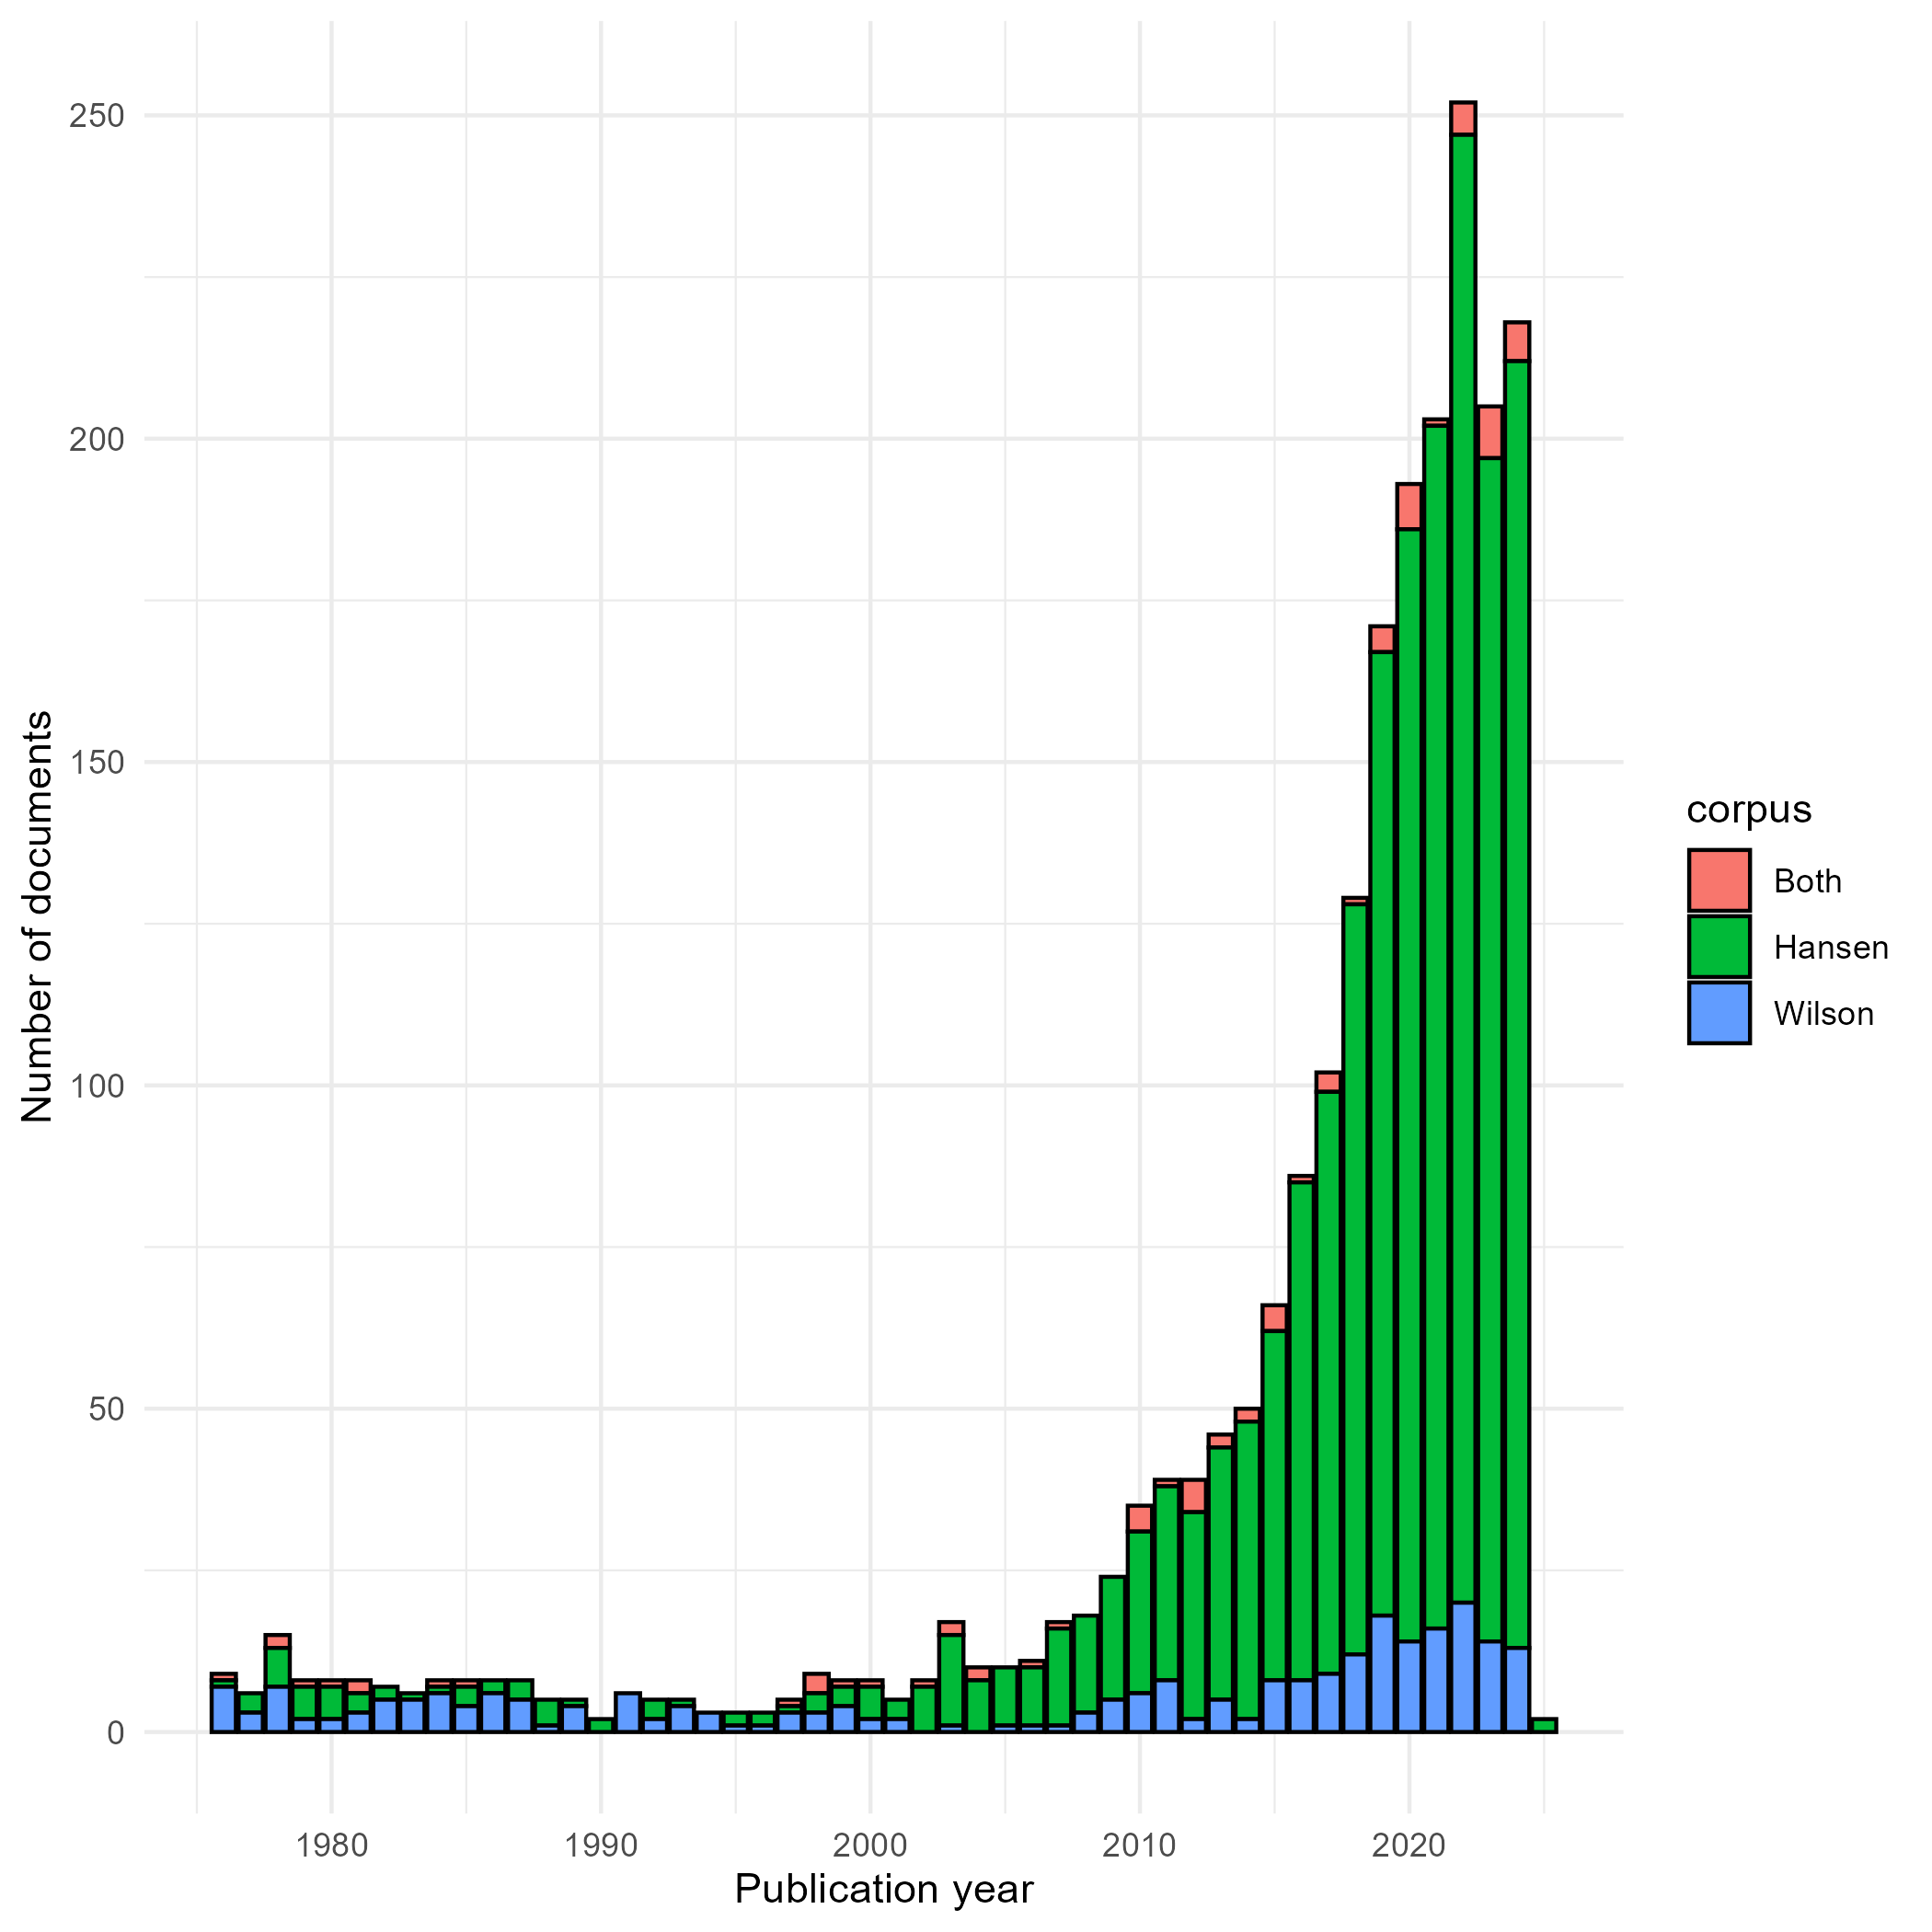
\includegraphics[width=0.7\linewidth]{data/figures/chp1-docs_per_year_plot} \caption{The count of articles, per year published, that city either Hansen 1959, Wilson 1971 or both.}\label{fig:chp1-fig-docs-per-year}
\end{figure}

To illustrate this point, we conducted a bibliographic analysis of the literature that cites Hansen (1959), Wilson (1971), or both. We retrieved all relevant documents using the Web of Science ``Cited References'' functionality, and the digital object identifiers of Hansen (1959) and Wilson (1971). As a result of this search, we identified 1,788 documents that cite Hansen (1959), only 258 documents that cite Wilson (1971), and 76 that cite both. The earliest document in this corpus dates to 1976 and the most recent is from 2025. The number of documents per year appears in Figure \ref{fig:chp1-fig-docs-per-year}, where we see the frequency of documents over a span of almost fifty years. In particular, we notice the remarkable growth in the number of papers that cite Hansen (1959) compared to those that cite Wilson (1971) since the year 2000.

As noted, literature that cites both Wilson (1971) and Hansen (1959) are sparse (only 3.6\% of the corpus, visualised in pink in Figure \ref{fig:chp1-fig-docs-per-year}). After reading the works, we can also discern that they too are divergent, with one stream focused on developing accessibility (i.e., \emph{potential for} spatial interaction) and another on spatial interaction. The focuses of these divergent streams contribute this paper's broader hypothesis that the concepts of accessibility and spatial interaction have remained largely disconnected, and at times, improperly conflated.

On one hand, the stream of literature focused on spatial interaction models inspired by Wilson (1971) and which cite both Hansen (1959) and Wilson (1971), tends to contribute to understanding how accessibility is interpreted and incorporated in spatial interaction models. These works treat separate spatial interaction and accessibility as a separate but related phenomenon. Specifically, some early works interpret the spatial interaction model's balancing factors (Equation \ref{eq:production-constrained-balancing-factor} or Equation \ref{eq:doubly-constrained-balancing-factors} as the inverse of Hansen (1959)`s model (A. Stewart Fotheringham, 1981; A. S. Fotheringham, 1985; B. Harris \& Wilson, 1978; G. Leonardi, 1978), recognizing it as a ``common sense'' approach (Morris, Dumble, \& Wigan, 1979, p. 99) to including accessibility in the spatial interaction model, though further exploration of its relationship is warranted (M. Batty \& March, 1976). Some authors have explored this relationship, for instance as in A. S. Fotheringham (1985) who demonstrates how the spatial interaction model may insufficiently explain spatial patterns, and suggests that explicitly defining destinations' accessibility as a variable within the model may remedy the issue (e.g., the \emph{competition destination} model). Other works used both Hansen (1959) and Wilson (1971)'s framework in conjunction, such as in defining location-allocation problems in operations research (Beaumont, 1981; G. Leonardi, 1978), estimating trip flows (or some other spatial interaction flows) alongside accessibility (Clarke, Eyre, \& Guy, 2002; Grengs, 2004; Türk, 2019), or considering accessibility within spatial interaction models, in line with A. S. Fotheringham (1985)'s demonstration (Beckers et al., 2022). Other works departed from Hansen (1959)'s definition and aligned with spatial interaction in different ways, such as using micro-economic consumer behaviour concepts to express potential for spatial interaction (Giorgio Leonardi \& Tadei, 1984; Morris et al., 1979).

On the other hand, there is another subset of literature that cite both Hansen (1959) and Wilson (1971) that is accessibility-focused. We categorise their citation of Wilson (1971) for three general reasons. Firstly, a group of these works cite Wilson (1971) as attribution for using context-dependent travel cost functions (Ashiru, Polak, \& Noland, 2003; Caschili, De Montis, \& Trogu, 2015; Chia \& Lee, 2020; Grengs, 2015; S. L. Handy \& Niemeier, 1997; Kharel, Sharifiasl, \& Pan, 2024; Kwan, 1998; Margarida Condeço Melhorado, Demirel, Kompil, Navajas, \& Christidis, 2016; Pan, 2013; Pan, Jin, \& Liu, 2020; Rau \& Vega, 2012; Roblot, Boisjoly, Francesco, \& Martin, 2021; Sharifiasl, Kharel, \& Pan, 2023; Q. Shen, 1998; J. W. Weibull, 1980). These works do not necessarily comment on spatial interaction explicitly. Secondly, another group of this accessibility-focused ``both'' citing literature \emph{does} associate spatial interaction as defined in Wilson (1971) with accessibility's potential for spatial interaction more explicitly (Giuliano, Gordon, Pan, \& Park, 2010; Grengs, 2010a, 2012; Grengs, Levine, Shen, \& Shen, 2010; He, Li, Yu, Liu, \& Huang, 2017; Levine, Grengs, Shen, \& Shen, 2012; Levinson \& Huang, 2012; X. Liu \& Zhou, 2015; H. J. Miller, 1999; Naqavi, Sundberg, Västberg, Karlström, \& Hugosson, 2023; Ng, Roper, Lee, \& Pettit, 2022; Suel et al., 2024; Tong, Zhou, \& Miller, 2015; Wu \& Levinson, 2020). We agree accessibility and spatial interaction are related topics: accessibility is an expression of its \emph{potential} and the Wilson (1971) paper briefly touches on the concept. However, in some of this literature, Hansen (1959) and Wilson (1971) are co-cited as both being `gravity models' (Chia \& Lee, 2020; Dai, Wan, \& Gai, 2017; S. Liu \& Zhu, 2004; Y. Shen, 2019), perhaps revealing the murkiness of the distinction between spatial interaction and the \emph{potential for} spatial interaction in the literature. Thirdly, there is a group of accessibility-focused works that interpret Hansen (1959)'s model as the singly- or doubly- constrained spatial interaction model's inverse balancing factor (R. W. Vickerman, 1974). This group cities the earlier spatial interaction works that make this connection and is especially prominent in the investigation of competitive accessibility topics (Albacete, Olaru, Paül, \& Biermann, 2017; Allen \& Farber, 2020; Alonso, Beamonte, Gargallo, \& Salvador, 2014; Chen \& Silva, 2013; Curtis \& Scheurer, 2010; El-Geneidy \& Levinson, 2011; Karst T. Geurs, van Wee, \& Rietveld, 2006; Karst \& Van Eck, 2003; Levinson \& Wu, 2020; Manaugh \& El-Geneidy, 2012; Marwal \& Silva, 2022; Mayaud, Tran, Pereira, \& Nuttall, 2019; Sahebgharani, Mohammadi, \& Haghshenas, 2019; Su \& Goulias, 2023; Willigers, Floor, \& van Wee, 2007). As outlined in preceding sections, we argue interpreting the singly- or doubly- constrained spatial interaction model's balancing factor as accessibility yields output values that are similarly plagued by interpretability issues.

Lastly, as an extension of the third reason within this group, only the works of Soukhov et al. (2023) and Soukhov et al. (2024) use Wilson (1971)'s balancing factors as a method for maintaining constraints on opportunities within the context of competitive accessibility. These works introduce the balancing factors as a mechanisms to ensure that opportunities at each destination are proportionally allocated to each zone (based on the proportion of population seeking opportunities and the relative travel impedance). This is to ensure that each zonal accessibility value is the sum of this proportional allocation from each destination, and that all zonal values ultimately sum to the total number of opportunities in the region. However, these balancing factors were deduced intuitively. These works do not explicitly state that the mathematical formulation of the equations are effectively equivalent to Wilson's singly constrained model (derived from entropy maximization); this equivalence was only discovered in hindsight. Soukhov et al. (2023) and Soukhov et al. (2024) also do not discuss the total constrained case or the accessible population variants of these different cases, which will be detailed in the next chapter.

\section{Chapter conclusion}\label{chapter-conclusion}

In this chapter, the Newtonian roots of human spatial interaction modelling was traced from Ravenstein (1885), to Hansen (1959)`s application of Stewart (1947)'s 'population potential' (Equation \ref{eq:stewart-population-potential}) and then to Wilson (1971)'s family of spatial interaction models. We detailed how the balancing factors from Wilson's family of spatial interaction models are formulated to reflect known system constraints (i.e., the total constraint, and production and attraction constraints in Equations \ref{eq:constraint0-gravitymodel}, \ref{eq:constraint1-gravitymodel} and \ref{eq:constraint2-gravitymodel}.

Literature that cite both seminal works is then reviewed (Hansen (1959) and Wilson (1971)). It is found that these works are divergent: some are spatial interaction focused, citing Hansen (1959) as the father of the accessibility concept and uses accessibility as a variable within spatial interaction modelling. Another set of work is accessibility focused, and what we may now know as the modern accessibility literature beginning in the early 2000s. These accessibility focused works cite Wilson (1971) for various general reasons, but none other than Soukhov et al. (2023) and Soukhov et al. (2024), cite the logic of the balancing factors. Beginning with this logic in the following chapter, balancing factors are introduced akin to those used in Wilson's family of spatial interaction models. They are formulated to incorporate system-wide or zonal constraints (i.e., knowns) to accessibility. In this way, the following chapter introduces a `family of accessibility measures'. Each member and variant of the family is mathematically formulated and solved using a simple toy example.

\chapter{A family of accessibility measures}\label{a-family-of-accessibility-measures}

\section{Overview}\label{overview-1}

This chapter consists of text from two journal articles. First, from the second half of the \emph{``Family of accessibility measures derived from spatial interaction principles''} authored by Anastasia Soukhov, Rafael H. M. Pereira, Christopher D. Higgins, and Antonio Páez (submitted to \emph{PLOS ONE} in May 2025) that details the formulation of the family of accessibility measures and solved simple numeric example. Second, the subsection ``a brief review of multimodal accessibility'' is pulled from the manuscript detailing the multimodal extension of spatial availability in the published article ``Multimodal spatial availability: A singly-constrained measure of accessibility considering multiple modes'' authorsed by Anastasia Soukhov, Javier Tarriño-Ortiz, Julio A. Soria-Lara, and Antonio Páez (Soukhov et al., 2024).

The objective of this chapter is to detail the formulation of the family of accessibility measures which are based on spatial interaction principles. These formulations are used in the next chapters of this dissertation.
This chapter first details four cases of the family: unconstrained, total constrained, singly constrained and doubly constrained accessibility measures. Each case has two variants, either accessible `opportunities' (i.e., the way Hansen (1959) is understood) or accessible `populations' (i.e., market potential, the way Reilly (1929) can be understood). An empirical example will be solved using the total constrained and singly constrained cases, so for these cases their multimodal extensions are defined. Lastly, a demonstration of a solved toy example is included following the formulation of each case and all the cases are summarised in the conclusion.

This chapter offers two general contributions:

\begin{itemize}
\tightlist
\item
  The formulaic specification of four cases of the family of accessibility measures, along with different variants and multimodal extensions: specifically, the unconstrained measure (i.e., Hansen-type measure), the total constrained measure (i.e., a constrained version of the Hansen-type measure), the singly constrained measure (i.e., related to the popular two step floating catchment approach (2SFCA)), and the doubly constrained measure representing realized interactions or `access', effectively equal to the doubly constrained spatial interaction model in formulation.
\item
  Summary of the interpretability advantages of the family using a worked simple toy example, as these constrained accessibility measures yield values in units of the number of potential ``opportunities for spatial interaction'' or ``population for spatial interaction'' for each zone and zonal flow.
\end{itemize}

\section{Outline of the family of accessibility measures}\label{outline-of-the-family-of-accessibility-measures}

As argued in the preceding chapter, the streams of research on accessibility and spatial interaction modelling have evolved as largely separate streams with little contact since Hansen (1959) and Wilson (1971). This may explain why the constraints and associated balancing factors of spatial interaction models did not cross over to accessibility analysis. This is intriguing since Wilson made an effort to connect developments in spatial interaction modelling to accessibility, noting for instance, the denominator of the proportionality constants specific to origins (Equation \ref{eq:production-constrained-balancing-factor}) is the inverse of balancing factor \(A_i\) (Wilson, 1971, p. 10):

\begin{equation}
\label{eq:Ai-as-accessibility}
S_i = \frac{1}{A_i} = \sum_j W_j^{(2)} f(c_{ij})
\end{equation} 

Understanding \(S_i\) as the inverse of Wilson's \(A_i\) does not uncover any new meaning for \(S_i\) itself. Indeed, mathematically it is true, \(A_i\)'s role in Wilson's general model \(T_{ij} = k W_i^{(1)} W_j^{(2)} f(c_{ij})\) is that of a balancing factor \(k\) i.e., keeping units balanced and proportionality based on constraints. Understanding \(S_i\) itself as a balancing factor is not wholly helpful as Hansen and (Stewart before him) defined accessibility as a partial sum of the demographic force \(F\) or the system-wide population potential of opportunities for spatial interaction (i.e., \(V_i = \sum_j \frac{M_j}{d_{ij}}\) after losing \(G\)).

Hence, we propose stepping back to introduce a revised definition of accessibility: the \emph{constrained} potential for spatial interaction. Once we bring back Wilson's proportionality constant \(k\) into the picture, we can define the \emph{potential for spatial interaction} between two locations \(i\) and \(j\) is as follows:

\begin{equation}
\label{eq:access-01}
V_{ij} = k W_j^{(2)} f(c_{ij})
\end{equation} 

\noindent where \(V_{ij}\) is the potential for interaction from \(i\) to \(j\). The accessibility from origin \(i\) can then be summarised as as a partial sum of the potential at \(i\):

\begin{equation}
\label{eq:accesssibility-01}
V_{i} = k \sum_j W_j^{(2)} f(c_{ij})
\end{equation} 

Similar to Equation \ref{eq:phys-gravity-model}, \(W_j^{(2)}\) above is the mass at the destination and the sub-indices are for \(i = 1,\cdots, n\) origins and \(j = 1,\cdots, m\) destinations.

The market potential variant can also be generally defined, which is effectively the transpose of \(i\) and \(j\) in Equation \ref{eq:access-01} and Equation \ref{eq:accesssibility-01} as follows:

\begin{equation}
\label{eq:market-01}
M_{ji} = k W_i^{(1)} f(c_{ij})
\end{equation} 

\begin{equation}
\label{eq:market-potential-01}
M_{j} = k \sum_j W_i^{(1)} f(c_{ji})
\end{equation} 

Similar to Equation \ref{eq:phys-gravity-model}, \(W_j^{(2)}\) above is the mass at the destination and the sub-indices are for \(i = 1,\cdots, n\) origins and \(j = 1,\cdots, m\) destinations.

To detail the anatomy of \(V_{ij}\) and \(M_{ji}\) along with the partial sums of \(V_i\) and \(M_j\), Figure \ref{fig:chp2-fig-analytical-device-conc-accessibility} illustrates the accessibility analytical framework we propose using a simple 3 zone system. Each measure's most disaggregate value is \(X_{ij}\), potential for spatial interaction from \(i\) to \(j\). The \(X\) is a stand in for the \(ij\) values of all the cases, their variants and multimodal extensions that will be described (i.e., \(V_{ij}^0, V_{ij}^{m0}, M_{ji}^0, M_{ji}^{m0}, V_{ij}^T, V_{ij}^{mT}, M_{ji}^T, M_{ji}^{mT}, V_{ij}^S, V_{ij}^{mS}, M_{ji}^S, M_{ji}^{mS}\) and \(V_{ij}^D, M_{ji}^D\)). The single marginals represent the origin-side and destination-side weights of the zones. The total marginal represent the sum of a single marginal.

\begin{figure}
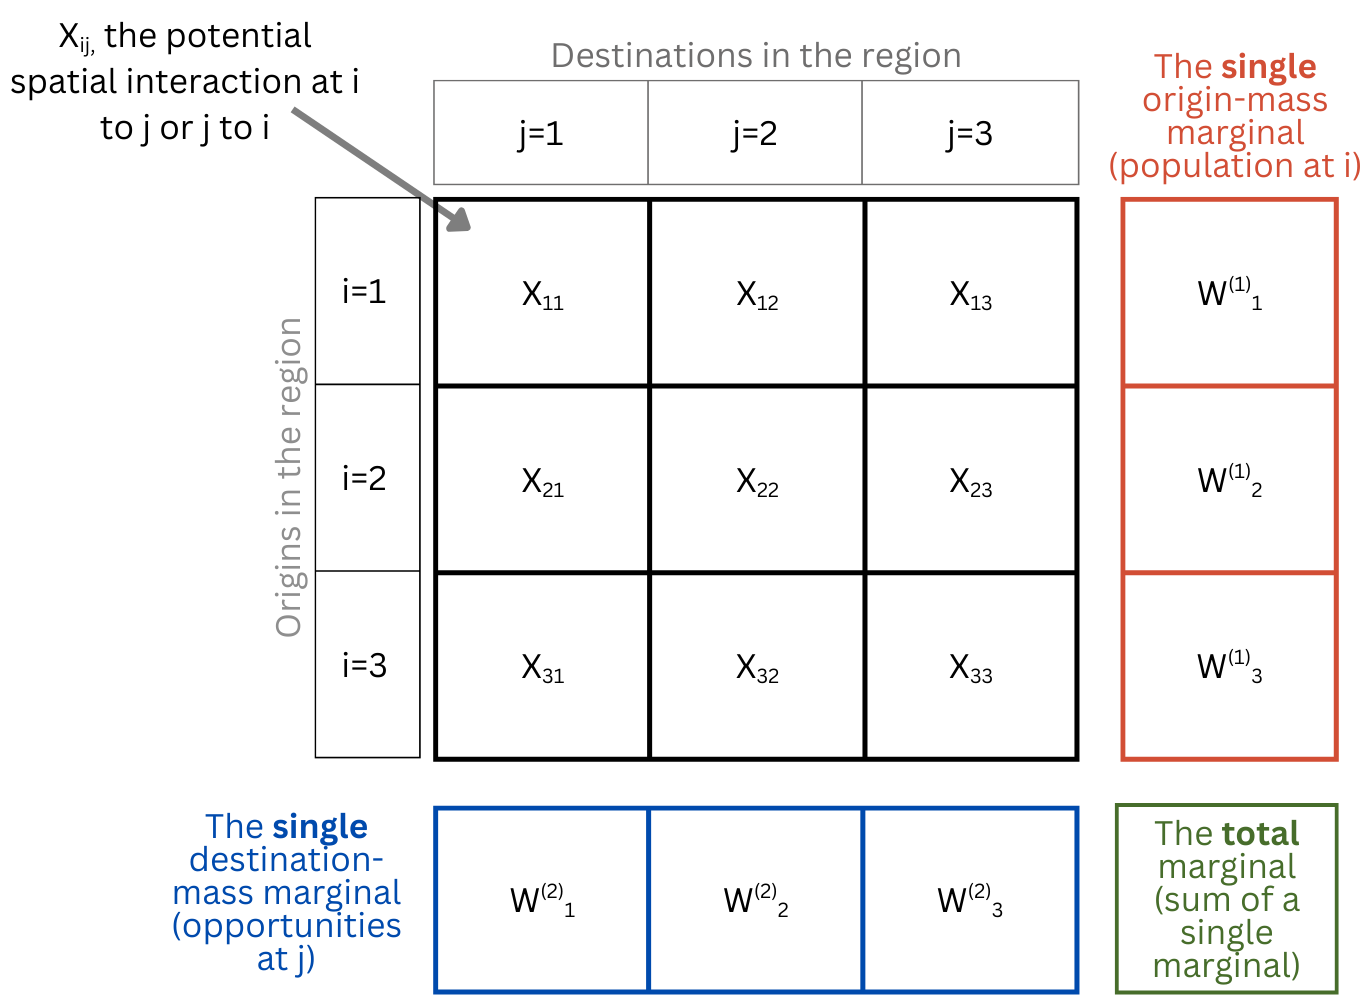
\includegraphics[width=0.7\linewidth]{data/figures/chp2-access-analytical-device} \caption{The family of accessibility measures analytical framework: labelling and associating ij flows, zonal weights, the single marginals, and the total marginal.}\label{fig:chp2-fig-analytical-device-conc-accessibility}
\end{figure}

As an additional overview, we define four distinct members of the constrained accessibility measure family, all delineated based on their constant \(k\), which takes the form of either balancing factors \(K^T\), \(B_j\), \(A_i\) (and their multimodal \(m\) versions) depending on the indicator:

\begin{enumerate}
\def\labelenumi{\arabic{enumi}.}
\item
  \textbf{The unconstrained case} with variants \(V_i^0\) and \(M_j^0\) and multimodal extension \(V_i^{m0}\) and \(M_j^{m0}\). The first variant \(V_i^0\) is equivalent to Hansen (1959)`s formulation and \(M_j^0\) is equivalent to Reilly (1929)'s market potential formulation. Both these variants neglect including a balancing factor, so units of zonal values are in units of 'opportunities-by-travel-impedance-value' and `population-by-travel-impedance-value'. In this case, no constraints are introduced to ensure that values of marginals are preserved.
\item
  \textbf{The total constrained case} with variant \(V_i^T\) and \(M_j^T\) along with multimodal extensions \(V_i^{mT}\) and \(M_j^{mT}\). The first variant \(V_i^T\)--the \emph{total constrained accessible opportunities measure}--resembles Hansen (1959)`s formulation but with an additional regional balancing factor \(K^T\) term, defined as the ratio of the total number of opportunities in the region to the total sum of unconstrained accessibility values in the region. In this way, \(K^T\) ensures that each zonal accessibility value is a proportion of the total opportunities in the region (i.e., the total marginal in Figure \ref{fig:chp2-fig-analytical-device-conc-accessibility}), requires no information about the population seeking opportunities, and is in units of 'opportunities' accessible. The second variant \(M_j^T\) is the transpose of \(i\) to \(j\) of the first variant, effectively a constrained version of market potential and is referred to as \emph{total constrained accessible population measure}. In this variant, each zonal accessibility value is a proportion of the total population in the region (maintained by \(\hat K^T\)), requires no information about the opportunities that are sought, and each zonal value is in units of `population' accessible.
\end{enumerate}

\begin{itemize}
\tightlist
\item
  When conceptualising \emph{potential} for spatial interaction--whether with opportunities or population--the total constrained case reflects the lowest level of restriction and hence maximum potential. The balancing factors \(K^T\) and \(\hat K^T\) only ensure that \(V_{ij}^T\) and \(M_{ji}^T\) values end up matching the \emph{total sum} of one of the single marginals, not the individual marginals themselves. For example, \(K^T\) does not guarantee that all the opportunities accessibility at \(V_{i=1}^T\) reflect a proportional allocation of the destination mass (i.e., \emph{number} of opportunities) at \(j=1, 2, 3\). In some cases, an allocation of opportunities from a destination \(j\) to \(i=1\) could \emph{exceed} the number of opportunities at that \(j\) (i.e., meaning that destination \(j\) is very attractive and reachable for an \(i\), relative other flows in the region). However, what \(K^T\) \emph{does} ensure is that each \(V_{ij}^T\) does not exceed the overall number of opportunities in the region--the total marginal. In other words, \(V_{i=1}^T\) expresses the number of opportunities that origin \(i=1\) could potentially interact with, as drawn from the entire regional opportunity mass, rather than constrained by individual destination totals. In this way, the \emph{total constrained} case reflects the maximum amount of \emph{potential} while still maintaining interpretable units.
\end{itemize}

\begin{enumerate}
\def\labelenumi{\arabic{enumi}.}
\setcounter{enumi}{2}
\tightlist
\item
  \textbf{The singly constrained case}, with two variants \(V_i^S\) (opportunity-constrained) and \(M_j^S\) (population-constrained) along with their multimodal extensions \(V_i^{mS}\) and \(M_j^{mS}\). The first variant is mathematically equivalent to the spatial availability measure (Soukhov et al., 2023), and this variant's per capita form is equivalent to the popular 2SFCA measure (Luo \& Wang, 2003; Q. Shen, 1998). Both variants can also be defined using either Hansen (1959)'s or the market potential formulation but with balancing factor \(B_j\) for \(V_i^S\) or \(A_i\) for \(M_j^S\). These balancing factors ensure that the total marginal (green box in Figure \ref{fig:chp2-fig-analytical-device-conc-accessibility}) is maintained \emph{as well as} the values at one of the single marginals (destination-mass marginal for opportunity-constrained and origin-mass marginal for population constrained in Figure \ref{fig:chp2-fig-analytical-device-conc-accessibility}). In this way, the singly constrained case reflects a medium amount of potential, restricted by either values fitting the single destination-mass marginal or the single origin-mass marginal.
\end{enumerate}

\begin{itemize}
\tightlist
\item
  The first variant \(V_i^S\) includes a set of destination-side balancing factors \(B_j\) which ensure opportunities (or destination masses) are allocated to each origin \(i\) based on the population (i.e, origin mass) of the origin \(i\) and travel impedance from that \(j\) to all \(i\)s. Hence, \(B_j\) ensures that each \(V_i^S\) is the product sum of a \emph{proportional share} of opportunities allocated from each destination \(j\) implicitly also being a share of the total opportunities in the region. Similar to the total constrained case, each \(V_i^S\) and \(V_ij^S\) accessibility value is expressed in units of `opportunities' accessible. But unlike the total constrained case, the singly constrained case explicitly incorporates population by allocating a balanced share of a destination's total opportunities to populations at reachable origins.
\item
  The second variant \(M_j^S\) includes a set of opportunity-side balancing factors \(A_i\) which ensure population (or origin masses) are allocated to each destination \(j\) based on the destination mass of the destination \(j\) and all possible travel impedance from that \(i\) to all \(j\)s. \(A_i\) ensures similar, but transposed, so constraints are satisfied. Specifically, each \(M_j^S\) represents both a share of the total regional population and the sum of balanced proportions of population from all origins, allocated to each destination based on the opportunities sought and travel impedance. Each zonal value is expressed in units of `population' accessible.
\end{itemize}

\begin{enumerate}
\def\labelenumi{\arabic{enumi}.}
\setcounter{enumi}{3}
\tightlist
\item
  \textbf{The doubly constrained case}. It is constrained simultaneously by population (origin masses) and opportunities (destination masses), so each \(V_{ij}^D\) (equivalent to \(M_{ji}^D\)) is expressed in units of `population-opportunity capacity' that is accessible between \(i\) to \(j\). This case requires the number of opportunities and population to match, e.g., the analyst must know the matching spatial interaction capacity of the population (demand) and opportunities (supply). By using this one-to-one matching data and the double constraints (i.e., \(A_i\) and \(B_j\) at once, ensuring both the double constraint maintains both marginals in Figure \ref{fig:chp2-fig-analytical-device-conc-accessibility}), this case restricts the \emph{potential} to spatially interact completely. In other words, the doubly constrained accessibility values reflect the number of predicted interactions between the opportunities and population, effectively, this case is equivalent formulaically as Wilson's doubly constrained spatial interaction model (i.e., \emph{attraction-production constrained}). It can be understood as predicting a value of `access', and not accessibility.
\end{enumerate}

And as a summary: each member of the family of accessibility measure is named, explained in plain language, alongside their balancing factor(s), proportional allocation factor(s), and mathematical equation and value interpretations in Table \ref{tab:summary-family-access-measures-table}.

{\tiny
\begin{longtable}{|p{1.2cm}|p{2cm}|p{3.8cm}|p{3.7cm}|p{2cm}|}
\caption{Summary of family of accessibility measure members, their definitions and interpretations} \label{tab:summary-family-access-measures-table} \\
\hline
\textbf{ } & \textbf{Unconstrained ($V_i^0$, $M_j^0$)} & \textbf{Total Constrained ($V_i^T$, $V_i^{mT}$, $M_j^T$, $M_j^{mT}$)} & \textbf{Singly Constrained ($V_i^S$, $V_i^{mS}$, $M_j^S$, $M_j^{mS}$)} & \textbf{Doubly Constrained ($V_{ij}^D$, $M_{ij}^D$)} \\
\hline
\endfirsthead

\textbf{Measure Equation} &
$V_i^0 = \sum_j W^{(2)}_j f(c_{ij})$;

$M_j^0 = \sum_i W^{(1)}_i f(c_{ij})$ 

&
$V^T_i = \sum_j  \kappa_{ij}^T W^{(2)}_j$;

$M_j^T =\sum_i \hat{\kappa}_{ji}^T  W^{(1)}_i$

Multimodal:

$V^{mT}_i = \sum_j \kappa_{ij}^{mT} D_j$;

$M_{mj}^T = \sum_i \hat{\kappa}_{ji}^{mT} O_i$ 

&
$V^S_i = \sum_j \kappa^S_{ij} D_j$;

$M_j^S = \sum_i \hat \kappa^S_{ji}  O_i$

Multimodal:

$V^{mS}_i = \sum_j \kappa_{ij}^{mS} W^{m(2)}_j$;

$M^{mS}_j = \sum_i \hat{\kappa}_{ji}^{mS} W^{m(1)}_i$ 

&
$V_{ij}^D = A_i B_j O_i D_j f(c_{ij})$ \\
\hline

\textbf{Constraint Explanation and Balancing Factor} &
No constraints; marginals not equal to any regional or zonal knowns.

Multimodal extension, where other modes $m$ are a function of $V_i^0$ and $M_j^0$ is not specified -- however, a specific $V_i^0$ and $M_j^0$ value for a mode can be expressed, and is represented as $V_i^{m0}$ and $M_j^{m0}$ 
&
Balancing factors $K^T$ and $\hat{K}^T$ ensures the sum of $ij$ values matches the total marginal, where:

$K^T = \frac{D}{\sum_i V_i^0}$;

$\hat{K}^T = \frac{O}{\sum_j M_j^0}$ 

Multimodal balancing factors ensuring the $ij$ matrix for each $m$ is a proportion of the marginal, where: 

$K^{mT} = \frac{D}{\sum_m\sum_i V_i^{m0}}$;

$\hat{K}^{mT} = \frac{O}{\sum_m\sum_j M_j^{m0}}$ 
&
Single balancing factor $B_j$ (for $V_i^S$) that ensures the destination-mass marginal is constrained, and $A_i$ (for $M_j^S$) ensures the origin-mass marginal is constrained:

$B_j = \frac{1}{\sum_i W_i^{(1)} f(c_{ij})}$;

$A_i = \frac{1}{\sum_j W_j^{(2)} f(c_{ij})}$ 

Multimodal extension:

$B_j^m = \frac{1}{\sum_m\sum_i W_i^{m(1)} f^m(c_{ij}^m)}$;

$A_i^m = \frac{1}{\sum_m\sum_j W_j^{(2)} f^m(c_{ij})^m}$ 
&
Values reflect both single marginals simultaneously, maintained via $A_i$ and $B_j$. 

Multimodal extension, where other modes $m$ are a function of $V_i^0$ and $M_j^0$ is not specified in this work -- however, balancing factors that are multimodal could be solved for, but is out of this work's scope. \\
\hline

\textbf{Propor-tional Allocation Factor} &
None &
Allocates the total marginal as opportunities proportionally based on $\kappa_{ij}^T = K^T f(c_{ij})$ and as population based on  $\hat{\kappa}_{ji}^T = \hat K^T f(c_{ij})$.

Multimodal extension:

$\kappa_{ij}^{mT} = B_j^m W_i^{m(1)} f^m(c_{ij}^m)$;
$\hat{\kappa}_{ji}^{mT} = A_i^m W_j^{m(2)} f^m(c_{ij}^m)$ 

&
Allocates the single opportunities marginal proportionally based on $\kappa^S_{ij} = B_j W_i^{(1)} f(c_{ij}) $ in the case of $V_i^S$ and the single population marginal proportionally based on $\hat \kappa^S_{ji} = A_i W_j^{(2)} f(c_{ij})$;

Multimodal extension:

$\kappa_{ij}^{mS} = B_j^m W_i^{m(1)} f^m(c_{ij}^m)$;
$\hat{\kappa}_{ji}^{mS} = A_i^m W_j^{m(2)} f^m(c_{ij}^m)$ 

&
— \\
\hline

\textbf{Interpret-ation} &
Values in various units depending on the impedance and destination-mass (e.g., "opportunities x decay") for $V_i^0$ and impedance and origin-mass (e.g., "population x decay"); no total or marginal constraint &
Values reflect a share of total regional opportunities ($V^T_i$) or population ($M^T_j$). &
$V^S_i$ values reflect a share of the opportunities at each destination based on origin population 'demand' and impedance; $M^S_j$ values reflect a share of the population at each origin based on destination opportunities 'supply' and impedance. &
The spatial interactions between population and opportunities (i.e., access). \\
\hline

\end{longtable}
}


\subsection{A brief review of multimodal accessibility measures}\label{a-brief-review-of-multimodal-accessibility-measures}

An important strength of a constrained accessibility framework is its ability to incorporate considerations of different subgroups of interaction behaviour of people with opportunities or opportunities with people, such as multiple modes of transportation. Measuring multimodal accessibility--that is, the potential to interact with opportunities through multiple modes--cannot be clearly defined using an unconstrained accessibility framework. Traditionally, Hansen-type methods have calculated unconstrained accessibility scores \(S_i^m\) separately for each mode and zone and then compared these values. However, as discussed when comparing unconstrained values across different analyses, this approach is similarly problematic because different modes often have distinct impedance functions, leading to differing units that obscure meaningful comparisons between modes. A solution is using a constrained approach: where multiple modal groups are considered within the same calculation and the total constraint and/or single constraint is satisified.

To cite an example from the literature of multimodal accessibility calculations using an unconstrained approach: Tahmasbi, Mansourianfar, Haghshenas, \& Kim (2019) uses unconstrained accessibility to assess the potential interaction with retail locations by three modes: walking, public transit, and car (i.e., \(m = w, p, c\)). \(S_i^m\) is the sum of retail locations \(j\) that can potentially be reached under the travel impedance as calculated for each \(i\) and \(m\). In other words, for each origin \(i\) three unconstrained accessibility scores are calculated. Tahmasbi et al. (2019) also shows that car travel affords the highest \(S_i^{m}\) values in the majority of \(i\) i.e., travelers who use a car can potentially reach more retail opportunities than populations using other modes. However, higher \(S_i^{m}\) values for car do not affect the values of \(S_i^{m}\) for other modes: in effect, each mode is analysed as if the others did not exist. Since the measure is not constrained, each opportunity is typically counted multiple times within and between modes, and as a result the sum of accessibility is not necessarily a meaningful quantity. The accessibility scores for the modes are often values that are difficult to interpret beyond making statements about relative size.

As another example, Lunke (2022) reports accessibility scores for car in the order of tens of thousands of employment opportunities in the Oslo region. The corresponding scores for transit are lower, but still often in the thousands or tens of thousands. As reported, the ratio of the transit to the car score can be lower than 0.2 (meaning transit gives access to less than 20\% of the opportunities than car). But despite the discussion about ``sufficient accessibility'', it is unclear what the unconstrained scores mean: is having access to 10,000 jobs by transit insufficient? After all, 10,000 employment opportunities are still plenty of opportunities. These ratios can be found elsewhere in the literature e.g., Figs. 7, 8, and 9 in A. Páez, Mercado, Farber, Morency, \& Roorda (2010), Fig. 5 in Antonio Páez et al. (2010), and Figs. 6, 7, and 8 in Antonio Páez et al. (2013). They are useful as relative assessment of when some members of the public are better or worse off than others, but they are silent on how bad is ``worse off''.

Besides ratios of accessibility, another method used in the literature to improve interpretability of scores is to standardise them within a {[}0-1{]} range. This adjustment is only helpful insofar as it facilitates relative comparisons, but interpretation of the scores remains challenging because the values are specific to a region and convey no meaning about the magnitude of the scores. In this approach, zones always have values between 0 and 1. However, how remarkable is a zone with a low score for pedestrians and a high value for car? And if remarkable, what does the difference in these standardized values mean for planners? By how much should transport systems and land-use configurations be changed to improve conditions? And in what way can these scores be used to track differences over time? Or between regions? These questions lack straightforward answers since certain values will always be relatively `low' or `high', but do not map onto a quantity that can be intuitively understood. Presentation or discussion of Hansen-type accessibility that has been standardised in this way is common in the literature (Campbell, Rising, Klopp, \& Mbilo, 2019; Maharjan, Tilahun, \& Ermagun, 2022).

If we understand opportunities to be finite and/or subject to some levels of congestion, it is possible for an accessibility measure to take on a crisper meaning. Accessibility research has a history of considering opportunity competition, especially regarding school-seats, hospital capacity, and employment opportunities (Cui et al., 2020; Grengs, 2010b; Higgs, Zahnow, Corcoran, Langford, \& Fry, 2017; Joseph \& Bantock, 1982; Kawabata \& Shen, 2006; Kelobonye, Zhou, McCarney, \& Xia, 2020; Kwok \& Yeh, 2004; C. Li \& Wang, 2024; Mao \& Nekorchuk, 2013; Merlin \& Hu, 2017; Morris et al., 1979; Q. Shen, 1998; Soukhov et al., 2023; Van Wee, Hagoort, \& Annema, 2001; Jörgen W. Weibull, 1976). If one person reaches an opportunity--it is taken: the supply of an opportunity and the demand for that opportunity are the nodes in accessibility analysis. These types of opportunities are unambiguously exclusive.

Amenities are a good example of this. For instance, standards for providing green spaces are often stated in the form of \emph{exclusive access}, in units of amenity per capita. For example, a 2013 planning document for the Ile-de-France region suggested a public green space municipal standard of 10 \(m^2\) \emph{per inhabitant} (Liotta, Kervinio, Levrel, \& Tardieu, 2020). Green spaces are not evenly distributed, meaning those who have access to them depends on where they are and how easy they are to reach. This formulation of amenity provision is not unusual. As another example, Natural England recommends a national ``accessible natural greenspace standard'' such that the minimum supply of space is 1 \(ha\) of statutory local nature reserves per thousand population (Natural England, 2010). Similarly, the World Health Organization (OECD, 2013) recommends that cities provide a minimum of 9 \(m^2\) of green area per inhabitant. For our purposes, standards of this type translate into ``how much of this resource is available to one individual that has not been claimed by anyone else?''. Green spaces often have large capacities, but they still have a capacity and it is not the same for a person to have access to 5 \(m^2\) of \emph{uncongested} green space as 15 \(m^2\). This difference is in fact a matter of justice (Lara-Valencia \& García-Pérez, 2015; Liotta et al., 2020). Constraining accessibility is a useful way to evaluate the congested availability of any type of opportunity. As development of sound standards is emphasized in the planning literature, in particular in regards to fairness in transportation (Martens \& Golub, 2021), spatial availability analysis can be used to develop and assess standards.

The relevance of the considerations above is put in sharper relief when we think about the use of multiple modes (or heterogeneous populations). If we return to Oslo for a moment (Lunke, 2022), we notice that the places that have high accessibility by transit are also the places that have \emph{very high} accessibility by car (in their Figure 2). Those two populations are going for the same opportunities, and those travelling by transit have fewer to choose from the start. More generally, people in a zone who are advantaged with relatively low cost of travel will have the ability to potentially reach more opportunities than other people. Due to this advantage, through the perspective of finite opportunities, there are fewer opportunities left for everyone else, especially for those who use modes that are slower or otherwise more expensive.

`Competitive' accessibility was the rationale for developing floating catchment area methods (FCA), popularized in Luo \& Wang (2003) who reformulated the work of Q. Shen (1998) into two steps (although similar, and earlier, developments are found in (Joseph \& Bantock, 1982; Jörgen W. Weibull, 1976)). Shen-type accessibility is formulated as: \(a_i^m = \sum_j \frac{O_jf^m(c_{ij}^m)}{\sum_m D_j^m}\) where \(D_j^m\) is the potential demand for opportunities equal to travel impedance weighted population \(\sum_i P_i^m f^m(c_{ij}^m)\) and the remaining variables are repeated in the Hansen-type measure. Shen-type modal accessibility (\(a_i^m\)) can be understood as a ratio of the travel impedance-weighted supply of opportunities for \(m\)-mode in \(i\) over the travel impedance-weighted demand for opportunities. In this way, it considers competition. That said, the measure remains unconstrained, meaning both population \emph{and} opportunities are multiply counted (Antonio Paez et al., 2019). In other words, interpretation of the Shen-type accessibility scores between modes is fraught, as it is for Hansen-type measures.

To illustrate, Tao et al. (2020) calculates \(a_i^m\) to jobs for different income-group populations in Shenzhen, China for those using transit and car. Their results indicate that zones with low-income populations have lower \(a_i^m\) than zones with higher-income populations. Further, they show that \(a_i^{\text{transit}}\) is lower than \(a_i^{\text{car}}\) in many zones, arguing that this may further place those zones with lower-income populations at a disadvantage. \(a_i\) and/or \(a_i^m\) are used to compare relative spatial differences in overall competitive accessibility and multimodal competitive accessibility, but because opportunities were doubly counted (entering the sums of both modes), this makes for uneasy interpretations of the differences in \(a_i^{m}\) between modes. Questions that this approach leaves unaddressed include: what is the impact of competition on the difference in \(a_i^m\) values? How does the impact vary spatially? And what is the interpretation of this difference?

The family of accessibility measures improves on the discussed Hansen-type and Shen-type accessibility approaches by constraining the sum of opportunities, that is, by treating them as finite and ensuring that the total constrained and/or the single constraint is satisfied. This is done by means of proportional allocation factors that follow well established principles of spatial interaction and the gravity model (Wilson, 1971). These principles consider: the cost of travel from different zones for a certain traveling group \(m\) compared to all groups (e.g., some sub-populations face relatively higher or lower costs), and if singly-constrained, the mass effect of \(m\) compared to all other \(m\)s e.g., the mass at different origins or destinations).

\section{Setup of the simple numeric example}\label{setup-of-the-simple-numeric-example}

Consider a simple region as shown in Figure \ref{fig:chp2-fig-analytical-device-conc-accessibility}, with zone IDs 1, 2 and 3. Each zone is both an origin \(i\) and a destination \(j\). The following three pieces of information are defined: zonal population and opportunities, zonal cost matrix, and travel impedance functions for three types of travel behaviour. In this example, the population are people, the opportunities are physicians, and the region can be described by three possible travel behaviours.

\begin{table}[!t]
\caption{Simple system with three zones (ID 1, 2 and 3). Population is in 10,000 persons and opportunities in number of physicians} \label{tab:chp2_small_system_land_use_tab}
\fontsize{7.5pt}{9.0pt}\selectfont
\begin{tabular*}{\linewidth}{@{\extracolsep{\fill}}rcc}
\toprule
ID (i or j) & Population\textsuperscript{\textit{1}} & Opportunities\textsuperscript{\textit{2}} \\ 
\midrule\addlinespace[2.5pt]
1 & 4 & 160 \\ 
2 & 10 & 150 \\ 
3 & 6 & 180 \\ 
\bottomrule
\end{tabular*}
\begin{minipage}{\linewidth}
\textsuperscript{\textit{1}}Population is \emph{Wi\textsuperscript{(1)}} when used as a proxy for the mass at the origin, and \emph{Oi} when used as a constraint.\\
\textsuperscript{\textit{2}}Opportunities is \emph{Wj\textsuperscript{(2)}} when used as a proxy for the mass at the destination, and \emph{Dj} when used as a constraint.\\
\end{minipage}
\end{table}



\begin{table}[!t]
\caption{Cost matrix for system with three zones (travel time in minutes)} \label{tab:chp2_small_system_land_use_cost_tab}
\fontsize{7.5pt}{9.0pt}\selectfont
\begin{tabular*}{\linewidth}{@{\extracolsep{\fill}}cccc}
\toprule
 & \multicolumn{3}{c}{Destination ID} \\ 
\cmidrule(lr){2-4}
Origin ID & 1 & 2 & 3 \\ 
\midrule\addlinespace[2.5pt]
1 & 10 & 30 & 15 \\ 
2 & 30 & 10 & 25 \\ 
3 & 15 & 25 & 10 \\ 
\bottomrule
\end{tabular*}
\end{table}



Firstly, Table \ref{tab:chp2_small_system_land_use_tab} summarises the population (in units of 10,000s of people) and the opportunities (the number of physicians) per zone. Considering Table \ref{tab:chp2_small_system_land_use_tab}'s values, the Provider-to-Population-Ratio (PPR) in this system is 24.5. For reference, the number of physicians per 10,000 in Canada in 2022 was 24.97 (WHO, 2025). Secondly, to pair the zonal population and opportunity information, the assumed cost of movement (in minutes of travel time) between origins and destinations is as shown in Table \ref {tab:chp2_small_system_land_use_cost_tab}.

From both Table \ref{tab:chp2_small_system_land_use_tab} and Table \ref {tab:chp2_small_system_land_use_cost_tab}, Zone 3 and 1 can be interpreted as of an urban core with major healthcare institutions and a healthcare cluster on the edge of the city respectively, each with a moderate residing population (with zone 3 having both a higher population and physician count). Zone 2, can be interpreted as a more distant bedroom community, with a relatively high population and fewer physicians. In sum, Zones 1 and 3 are more proximate to each other than to Zone 2, and together match Zone 2's population while offering more than twice the physician availability.

And lastly, in Equation \ref{eq:travel-behaviour-scenarios} we distinguish accessibility measure values for the following three impedance functions that represent the potential for spatial interaction travel behaviour of the population to opportunities. Accessibility will be calculated three times for each case, one assuming the most decay (\(f_1(c_{ij})\)), another assuming medium decay (\(f_2(c_{ij})\)), and a third assuming the least decaying travel behaviour (\(f_3(c_{ij})\)) for the entire region. A helpful analogy may be tying travel behaviour to the used mode's mobility potential, i.e., the most decaying travel behaviour (\(f_1(c_{ij})\)) would assume all travel in the region being done by foot, while calculating accessibility assuming the least decay (\(f_3(c_{ij})\)) would assume unfettered automobility. Or alternatively, these functions could represent travel behaviour on snowstorm-affected day (\(f_1(c_{ij})\)) for the entire region versus a clear, ideal travel day (\(f_3(c_{ij})\)). As an example of a discussion on how travel behaviour has been considered in accessibility measures cost of travel see A. Paez, Scott, \& Morency (2012).

\begin{equation}
\label{eq:travel-behaviour-scenarios}
\begin{array}{l}
f_1(c_{ij}) = \frac{1}{c_{ij}^3}\\
f_2(c_{ij}) = \frac{1}{c_{ij}^2}\\
f_3(c_{ij}) = \frac{1}{c_{ij}^{0.1}}
\end{array}
\end{equation} 

Any set of concepts representing population, opportunities, and their associated travel behaviour, whether representing the entire region uniformly (as we will demonstrate) or representing specific subgroups, can be substituted into our simple example, depending on the research question. The purpose of the following simple example is to demonstrate the calculation of each member of the accessibility measure family, interpret the values, and compare them both within and across travel behaviour groups and members of the family of accessibility measures.

\section{Unconstrained accessibility}\label{unconstrained-accessibility}

Setting the balancing factor \(k\) to 1 or omitting it completely in Equation \ref{eq:access-01} results in the unconstrained accessibility case:

\begin{equation}
\label{eq:unconstrained-access}
V^0_{ij} = 1 *W_j^{(2)} f(c_{ij})
\end{equation} 

In this case, the partial sum of spatial interaction is simply identical to Hansen's accessibility \(S_i\) (Hansen, 1959), the current standard practice in accessibility measurement:

\begin{equation}
\label{eq:unconstrained-accessibility}
V^0_i = \sum_j V^0_{ij} = \sum_j W^{(2)}_jf(c_{ij}) = S_i
\end{equation} 

The sum of the unconstrained accessibility values for each origin \(V^0_{i}\) generally does not equal the total number of opportunities \(O\) (e.g., \(\sum_i V^0_{i} \not= O\)), since arbitrarily setting \(k\) to 1 (or neglecting \(k\) all together) strips the values of any meaningful unit-based interpretation, the units are in `summed opportunities by some travel impedance value'. Moreover, comparisons of these \(V^0_{i}\) values across different contexts such as different impedance functions \(f(c_{ij})\) or varying number of zones exacerbates this issue as the units between \(V^0_{i}\) values change i.e., comparisons between a value of `summed opportunities by a travel impedance value' to a value of `summed opportunities by another travel impedance value' are not directly interpretable. From this perspective, the raw unconstrained accessibility scores are not intuitively comparable across different contexts and decay functions. They should more appropriately be used as an ordinal variable to make comparisons of size (i.e., greater than, less than, equal to), not to calculate ratios or intervals (i.e., the magnitude of differences).

The multimodal version of unconstrained accessibility can be represented as \(V^{m0}_{i}\) (Equation \ref{eq:unconstrained-multimodal-accessibility}) for each mode \(m\) assuming mode-specific impedance functions \(f^m(c^m_{ij})\). However, variables of other modes (i.e., summation of all \(m\), etc.) are not included in the equation, so \(V^{m0}_{i}\) is effectively equivalent to \(V^0_{i}\)--except \(m\) makes explicit that there are multiple groups at each \(i\) and those groups have their own \(V^0_i\) values based on \(f^m(c^m_{ij})\). There is no consistent approach of representing \(V^0_{i}\) as a function of multiple modes, other than averaging \(i\) values or other post hoc adjustments that generally do not preserve known properties of the system. From this perspective, as \emph{other} \(m\) values are not incorporated into the measure, we assume \(V^0_{i}\) cannot be made multimodal, and only \(V^0_{i}\), as calculated for different \(m\)s is used in this work.

\begin{equation}
\label{eq:unconstrained-multimodal-accessibility}
V^{m0}_{i} = \sum_j V^{m0}_{ij} =  \sum_j W_j^{(2)} f^m(c^m_{ij})
\end{equation} 

Returning to our numeric example, the calculated unconstrained accessibility \(V^0_{i}\) for each origin, a sum of all the travel impedance weighted opportunities at each destination (\(\sum_i V^0_{i}\)), in displayed in Table \ref{tab:chp2_simple_example_unconc_access_tab}.

\begin{table}[!t]
\caption{Simple system: unconstrained accessibility} \label{tab:chp2_simple_example_unconc_access_tab}
\fontsize{7.5pt}{9.0pt}\selectfont
\begin{tabular*}{\linewidth}{@{\extracolsep{\fill}}>{\raggedright\arraybackslash}p{\dimexpr 45.00pt -2\tabcolsep-1.5\arrayrulewidth}|>{\centering\arraybackslash}p{\dimexpr 135.00pt -2\tabcolsep-1.5\arrayrulewidth}>{\centering\arraybackslash}p{\dimexpr 135.00pt -2\tabcolsep-1.5\arrayrulewidth}>{\centering\arraybackslash}p{\dimexpr 135.00pt -2\tabcolsep-1.5\arrayrulewidth}}
\toprule
 & \multicolumn{3}{>{\centering\arraybackslash}m{\dimexpr 405.00pt -2\tabcolsep-1.5\arrayrulewidth}}{V\textsubscript{i}\textsuperscript{0}} \\ 
\cmidrule(lr){2-4}
 & f\textsubscript{1} (c\textsubscript{ij}) = 1/c\textsubscript{ij}\textsuperscript{3} & f\textsubscript{2} (c\textsubscript{ij}) = 1/c\textsubscript{ij}\textsuperscript{2} & f\textsubscript{3} (c\textsubscript{ij}) = 1/c\textsubscript{ij}\textsuperscript{0.1} \\ 
\cmidrule(lr){2-2} \cmidrule(lr){3-3} \cmidrule(lr){4-4}
Origin & units: \emph{physicians-minute\^{}-3} & units: \emph{physicians-minute\^{}-2} & units: \emph{physicians-minute\^{}-0.1} \\ 
\midrule\addlinespace[2.5pt]
1 & 0.219 & 2.567 & 371.143 \\ 
2 & 0.167 & 1.966 & 363.479 \\ 
3 & 0.237 & 2.751 & 373.738 \\ 
\midrule 
\midrule 
Sum & 0.6233422 & 7.283556 & 1108.361 \\ 
\bottomrule
\end{tabular*}
\end{table}



As the different impedance functions represent different travel behaviours, comparing the raw unconstrained accessibility values across groups is meaningless beyond notions of higher or lower. For instance, at zone 1 the difference between the least decay (\(f_3(c_{ij})\)) and most decay (\(f_1(c_{ij})\)) groups is 370.92, but in what units? These two values are a product of different impedance functions, making the comparison uninterpretable in absolute terms. Likewise, we could compare values within the same travel behaviour scenario across different zones, as they are in the same units, however the issue of unit interpretability will also be apparent. Considering the most decaying scenario \(f_1(c_{ij})\) and zone 1 (the zone with a healthcare cluster at the edge of the city): zone 1 captures 0.0181185 fewer physicians-minute\(^{-1}\) than zone 3 (urban core). Again, the fundamental uninterpretability of what is a \emph{physicians-minute\(^{-1}\)} or \emph{opportunity-weighted-travel-impedance} unit remains.

Moving onto the market potential variant, it is the transpose (\(i\) to \(j\)) of \(V^0_{ij}\) and depicted as follows:

\begin{equation}
\label{eq:unconstrained-market}
M_j^0 = \sum_i M^0_{ji} = \sum_i W_i^{(1)} f(c_{ij})
\end{equation} 

Where \(M^0_{ji}\) is the number of population-\(f(c_{ij})\) at each \(j\) from \(i\). It can be summarised for each \(j\) and hence expressed as \(M^0_j\).

The multimodal extension of \(M^0_{ji}\) can also be defined as follows:

\begin{equation}
\label{eq:unconstrained-multimodal-accessibility}
M^{m0}_{j} = \sum_i M^{m0}_{ji} =  \sum_i W_i^{(1)} f^m(c^m_{ij})
\end{equation} 

For the sake of brevity, the simple example is not solved for \(M_j^0\): results are similarly unconstrained as shown in the unconstrained accessible population demonstration.

In sum, multimodal extensions \(V^{m0}_{i}\) and \(M^{m0}_{j}\) for the simple example are also not solved here, but for a different reason. Namely, they are not truly `multimodal', as they are not a function of \emph{all} modes in the system. Instead, one must attempt to adjust the units post-calculation (e.g., scaling, normalization) or select impedance functions to facilitate comparison across scenarios (potentially at the expense of accurately reflecting travel behavior) and such adjustments may introduce bias. Hence, the raw unconstrained accessibility values themselves are challenging to compare due to their units. To enable more meaningful comparison, the following sections will detail the introduction of constraining constants to ensure consistent units across scenarios and demonstrate results on the same numeric example.

\section{Total constrained accessibility}\label{total-constrained-accessibility}

In the total constrained accessibility case, a total balancing factor proportionally adjusts unconstrained zonal accessibility values \(V^0_i\) based on the regional sum of \(V^0_i\) and the total population or opportunities in the region. Alternatively, we reformulate this case using a proportional allocation constant, which allocates opportunities (or population) proportionally based on the the travel impedance and the total population or opportunities in the region. In both formulations, all zonal values become a proportion of a known system total, be it the regional opportunities or regional population depending on the variant.

We define two variants for this case: (a) \(V_i^T\) where accessibility is constrained by the total number of opportunities (total constrained accessible opportunity) and which is interpreted as Hansen's accessibility with a constraining constant, and (b) \(M_j^T\), where \(i\) and \(j\) of the first variant is transposed, yielding a measure constrained by the total number of population and to be interpreted as constrained `market potential'. Following these definitions, these variants are extended into their multimodal expressions, considering multiple travel behaviour groups or modes \(m\).

\subsection{Total constrained accessible opportunities: Hansen's accessibility with a total constraint}\label{total-constrained-accessible-opportunities-hansens-accessibility-with-a-total-constraint}

Unlike in Equation \ref{eq:access-01}, the proportionality constant \(k\) is retained. For the total constrained case, it is represented as \(K^T\):

\begin{equation}
\label{eq:total-constrained-access}
V^T_{ij} = K^T \cdot W_j^{(2)} \cdot f(c_{ij})
\end{equation} 

In this way, the total constrained accessibility measure now becomes Hansen's accessibility with a balancing factor \(K^T\):

\begin{equation}
\label{eq:total-constrained-accessibility}
V^T_i = \sum_j V^T_{ij} = K^T \sum_j W^{(2)}_jf(c_{ij}) = K^T \cdot V^0_i
\end{equation} 

Imagine that the only system known is the total number of opportunities \(D\) in the region. Accordingly, the constant we impose in this case ensures the regional sum of total constrained accessibility is equal to the total number of opportunities as follows:

\begin{equation}
\label{eq:total-constraint-accessibility}
\sum_i V^T_{i} = \sum_i\sum_j V^T_{ij} = D
\end{equation} 

This constraint is analogous to the total constraint of Equation \ref{eq:constraint0-gravitymodel}, congruent with Wilson's framework. Given the total number of opportunities in the region, we can then substitute Equation \ref{eq:total-constrained-accessibility} in Equation \ref{eq:total-constraint-accessibility} to solve for \(K^T\):

\begin{equation}
\label{eq:total-opportunity-balancing-factor}
K^T =\frac{D}{\sum_i\sum_j V^0_{ij}} = \frac{D}{\sum_i\sum_j W^{(2)}_jf(c_{ij})}
\end{equation} 

Which is also congruent with Wilson's framework as it comparable to the total flow spatial interaction model (e.g., Equation 2.11 in Cliff et al. (1974)). Hence, rearranging the equation to have opportunities and the proportional constant distinctly represented, our total constrained accessibility model is:

\[
V^T_i = K^T\sum_j W^{(2)}_jf(c_{ij}) = \sum_j W^{(2)}_j\frac{D\cdot f(c_{ij})}{\sum_i\sum_j W^{(2)}_jf(c_{ij})}
\]

Further, we can see that, since \(D\) and \(W^{(2)}_j\) are both in units of opportunities, the proportional allocation factor for the total constrained opportunity case \(\kappa_{ij}^T\) is dimensionless:

\[
\kappa_{ij}^T = \frac{D\cdot f(c_{ij})}{\sum_i\sum_j W^{(2)}_jf(c_{ij})}
\]
\noindent and therefore \(V^T_i\) is now in the units of \(W^{(2)}_j\), that is, the mass at the destination (\(V^T_i = \kappa_{ij}^T\sum_j W^{(2)}_j\)). The role of \(\kappa_{ij}^T\) in this reformulation of accessibility is to transform between units and to adjust the number of opportunities accessible from \(i\) so they represent a proportion of the total number of opportunities in the region. \(\kappa_{ij}^T\) then assigns opportunities in proportion to the impedance between \(i\) and \(j\). This is why we refer to \(\kappa_{ij}^T\) as a proportional allocation factor. On the other hand, the proportionality constant \(K^T\) balances the units of \(V^0_i\), the Hansen-type accessibility values, and is an alternative expression of the total constrained accessibility measure.

Referring back to our simple numeric example, balancing factor \(K^T\) for the most decay travel behaviour scenario \(f_1(c_{ij}) = 1/c_{ij}^3\) would then be:
\[
\begin{array}{l}
K^T = \frac{D}{\sum_{i}\sum_{j} W_j^{(2)} f(c_{ij})}\\
K^T = \frac{D}{\frac{W_1^{(2)}}{c_{11}^3}+\frac{W_1^{(2)}}{c_{21}^3} + \frac{W_1^{(2)}}{c_{31}^3} + \cdots + \frac{W_3^{(2)}}{c_{31}^3} + \frac{W_3^{(2)}}{c_{32}^3} + \frac{W_3^{(2)}}{c_{33}^3}
}\\
K^T = \frac{490}{0.6233422} \\
K^T = 786.085
\end{array}
\]

\(K^T\) for the lower decay scenarios \(f_2(c_{ij}) = 1/c_{ij}^2\) and \(f_3(c_{ij}) = 1/c_{ij}^0.1\) are 67.2748352 and 0.4420944 respectively.

Using the calculated balancing factors for all zones and multiplying them by the unconstrained accessibility value \(V^0_i\), the total opportunity constrained accessibility values for all zones and different travel behaviour scenarios is presented in Table \ref{tab:chp2_simple_example_total_opp_access_tab}. \(\kappa_{ij}^T\) for each zone is not reported, but can be understood to be the unitless proportion of opportunities (of the total opportunities) allocated to each zone based on travel impedance.

\begin{table}[!t]
\caption{Simple system: total constrained accessible opportunities} \label{tab:chp2_simple_example_total_opp_access_tab}
\fontsize{7.5pt}{9.0pt}\selectfont
\begin{tabular*}{\linewidth}{@{\extracolsep{\fill}}>{\raggedright\arraybackslash}p{\dimexpr 45.00pt -2\tabcolsep-1.5\arrayrulewidth}|>{\centering\arraybackslash}p{\dimexpr 135.00pt -2\tabcolsep-1.5\arrayrulewidth}>{\centering\arraybackslash}p{\dimexpr 135.00pt -2\tabcolsep-1.5\arrayrulewidth}>{\centering\arraybackslash}p{\dimexpr 135.00pt -2\tabcolsep-1.5\arrayrulewidth}}
\toprule
 & \multicolumn{3}{>{\centering\arraybackslash}m{\dimexpr 405.00pt -2\tabcolsep-1.5\arrayrulewidth}}{V\textsubscript{i}\textsuperscript{T}} \\ 
\cmidrule(lr){2-4}
 & f\textsubscript{1} (c\textsubscript{ij}) = 1/c\textsubscript{ij}\textsuperscript{3} & f\textsubscript{2} (c\textsubscript{ij}) = 1/c\textsubscript{ij}\textsuperscript{2} & f\textsubscript{3} (c\textsubscript{ij}) = 1/c\textsubscript{ij}\textsuperscript{0.1} \\ 
\cmidrule(lr){2-2} \cmidrule(lr){3-3} \cmidrule(lr){4-4}
Origin & units: \emph{physicians} & units: \emph{physicians} & units: \emph{physicians} \\ 
\midrule\addlinespace[2.5pt]
1 & 172.065 & 172.672 & 164.080 \\ 
2 & 131.627 & 132.247 & 160.692 \\ 
3 & 186.308 & 185.081 & 165.228 \\ 
\midrule 
\midrule 
Sum & 490 & 490 & 490 \\ 
\bottomrule
\end{tabular*}
\end{table}



In contrast to unconstrained accessibility \(V^0_i\), imposing a constraint--in this case a total opportunity constraint for this variant--allows for the comparison of differences and ratios between regions and across different travel behaviour scenarios as well. Each value is effectively in units of physicians, with the impedance units already accounted for by \(\kappa_{ij}^T\).

Considering the highest decay scenario (\(f_1(c_{ij})\)), zone 1 (a healthcare cluster at the edge of the city) captures an intermediate amount of physicians (172.0652825) like in the unconstrained accessibility case. However, unlike in the unconstrained case, we can say that this value is out of the 490 physicians in the region, which allows us also to deduce that zone 1 captures 1.3072213 and 0.9235529 times more than zone 2 and 3. Values for the lesser decay (\(f_2(c_{ij})\)) and lowest decay (\(f_3(c_{ij})\)) scenarios are calculated separately, with decay scenario values also summing to equal 490 physicians accessible in the region.

One can also directly compare values at a specific zone due to the consistent units. For instance, zone 1 remains intermediate in capturing accessible physicians relative to zones 2 and 3 across scenarios, similar to the unconstrained case. However, the difference between travel behaviour scenarios differ in direction. Specifically, Zone 1 captures 0.6067946 more and 7.9850478 fewer opportunities than the lesser decay scenarios \(f_2(c_{ij})\) and \(f_3(c_{ij})\) respectively. Why? \(\kappa_{ij}^T\) ensures proportional allocation for each travel behaviour scenario. Meaning, while the unconstrained accessibility increases, \(\kappa_{ij}^T\) adjusts the values to remain proportional to the total number of opportunities (490 physicians accessible in the region). As the decay behaviour decreases, more opportunities are accessible for all zones. In the medium decay scenario \(f_2(c_{ij})\), zone 1 sees a slight increase in values (relative to the highest decay scenario) as the zone can accessible more opportunities relative to increases seen in other zones. However, in the lowest decay scenario, zone 1 sees a decrease, as it is outpaced by increases in other zones - namely zone 2 (recall: zone 2 has the lowest number of opportunities, hence the increases in opportunity gains is much higher in a low decay scenario).

Using the total opportunity constrained formulation of accessibility offers a solution to the unit interpretability issue of Hansen (1959)'s accessibility measure. Intuitively, the use of the constraint illustrates how the differences and ratios of values between zones and decay groups can be compared. This is true for other constrained cases of the family of accessibility measures.

\subsection{Total constrained accessible population: Reilly's potential trade territories with a total constraint}\label{total-constrained-accessible-population-reillys-potential-trade-territories-with-a-total-constraint}

Another variant of the total constrained accessibility measure is the \emph{total constrained accessible population measure}, which represents the transpose of \(i\) to \(j\) of the total constrained accessible opportunities measure. This variant, expressed in Equation \ref{eq:total-constrained-market}, represents an expression of the concept of market potential (i.e., potential users) as proposed in C. D. Harris (1954) and R. W. Vickerman (1974), and which Reilly earlier referred to as `potential trade territories' (Reilly, 1929). This unconstrained form of market potential \(M_j^0\) (Equation \ref{eq:unconstrained-market}), effectively the \(i\) to \(j\) transpose of \(V^0_{ij}\), has been used in recent research to express the potentially accessible population (i.e., users) as a result of regional transportation infrastructure investment projects (Condeço-Melhorado \& Christidis, 2018; Gutiérrez, 2001; Holl, 2007). Put another way, market potential can also be thought of as a form of \emph{passive accessibility}, indicating the number of people that can reach each destination. However, like \(V_{ij}^0\), issues of unit interpretability arise in \(M_j^0\)'s unconstrained form. To address this, the constrained variant, the total constrained accessible population measure \(M^T_{j}\), is introduced. To formulate this variant, the total balancing factor \(K^T\) is applied to the mass of the \emph{population} at \(i\) (\(W_i^{(1)}\)) instead of the opportunities at \(j\).

\begin{equation}
\label{eq:total-constrained-market}
M^T_{j} = \sum_i M^T_{ij} = \hat K^T \sum_i W_i^{(1)} f(c_{ij}) = \hat K^T M_{j}^0
\end{equation} 

Where we impose the total system known as a constraint, i.e., that the total market potential equals the total population \(O\) in the region:

\begin{equation}
\label{eq:total-constraint-market}
\sum_j M^T_{j} = \sum_i\sum_j M^T_{ji} = O
\end{equation} 

Substituting Equation \ref{eq:total-constrained-market} in Equation \ref{eq:total-constraint-market}, and solving for \(\hat K^T\), we obtain:

\begin{equation}
\label{eq:total-population-balancing-factor}
\hat K^T=\frac{O}{\sum_i\sum_i M^T_{ji}} = \frac{O}{\sum_i\sum_j W^{(1)}_i f(c_{ij})} 
\end{equation} 

The constrained market potential then takes the following form:
\[
M^T_j = \hat K^T\sum_i W^{(1)}_if(c_{ij}) = \sum_i W^{(2)}_i \frac{O \cdot f(c_{ij})}{\sum_i\sum_j W^{(2)}_if(c_{ij})}
\]

Where the following \(\hat \kappa_{ji}^T\) proportional allocation factor is dimensionless:
\[
\hat \kappa_{ji}^T = \frac{\sum_i O \cdot f(c_{ij})}{\sum_i\sum_j W^{(2)}_if(c_{ij})}
\]

Returning back to the numerical example, the proportionality constant \(\hat K^T\) is solved for each travel behaviour scenario, and the market potential of each zone \(M^T_j\) is expressed as units of population (e.g., the number of people accessible from each origin at that destination) in Table \ref{tab:chp2_simple_example_total_pop_market_tab}.

\begin{table}[!t]
\caption{Simple system: total constrained accessible population.} \label{tab:chp2_simple_example_total_pop_market_tab}
\fontsize{7.5pt}{9.0pt}\selectfont
\begin{tabular*}{\linewidth}{@{\extracolsep{\fill}}>{\raggedright\arraybackslash}p{\dimexpr 67.50pt -2\tabcolsep-1.5\arrayrulewidth}|>{\centering\arraybackslash}p{\dimexpr 112.50pt -2\tabcolsep-1.5\arrayrulewidth}>{\centering\arraybackslash}p{\dimexpr 112.50pt -2\tabcolsep-1.5\arrayrulewidth}>{\centering\arraybackslash}p{\dimexpr 112.50pt -2\tabcolsep-1.5\arrayrulewidth}}
\toprule
 & \multicolumn{3}{>{\centering\arraybackslash}m{\dimexpr 337.50pt -2\tabcolsep-1.5\arrayrulewidth}}{M\textsubscript{i}\textsuperscript{S}} \\ 
\cmidrule(lr){2-4}
 & f\textsubscript{1} (c\textsubscript{ij}) = 1/c\textsubscript{ij}\textsuperscript{3} & f\textsubscript{2} (c\textsubscript{ij}) = 1/c\textsubscript{ij}\textsuperscript{2} & f\textsubscript{3} (c\textsubscript{ij}) = 1/c\textsubscript{ij}\textsuperscript{0.1} \\ 
\cmidrule(lr){2-2} \cmidrule(lr){3-3} \cmidrule(lr){4-4}
Destination & units: \emph{population in 10,000s} & units: \emph{population in 10,000s} & units: \emph{population in 10,000s} \\ 
\midrule\addlinespace[2.5pt]
1 & 5.018 & 5.447 & 6.598 \\ 
2 & 8.596 & 7.986 & 6.717 \\ 
3 & 6.386 & 6.567 & 6.684 \\ 
\midrule 
\midrule 
Sum & 20 & 20 & 20 \\ 
\bottomrule
\end{tabular*}
\end{table}



Readers may note the difference in trends in accessible population (Table \ref{tab:chp2_simple_example_total_pop_market_tab}, immediately above) and the preceeding accessible physicians (Table \ref{tab:chp2_simple_example_total_opp_access_tab}). In the accessible population Table \ref{tab:chp2_simple_example_total_pop_market_tab}, zone 1, 2, 3 represent destinations and the accessibility values reflect the number of accessible people from the vantage of physicians. Zone 1, in its role as a destination, is no longer intermediately-ranked relative to other zones; it now attracts the fewest number of people across all three travel behaviour scenarios. However, similar to the total constrained opportunity case, as travel decay reduces, the availability of population begins to converge (though Zone 1 continues as the lowest-ranked) for similar reasons. As decay reduces, the population's travel impedance to all zones become more similar, making the relative location of the zones less important and all people in the region more equally accessible. Overall: like the total constrained accessible opportunities case, this variant allows for the interpretation of both ordinal and interval comparisons of the raw values themselves.

\subsection{Multimodal extension of total constrained accessible opportunities and population}\label{multimodal-extension-of-total-constrained-accessible-opportunities-and-population}

Having detailed both variants \(V_i^T\) and \(M_j^T\), their multimodal extensions can now be introduced. This extension is relevant if one is interested in accounting for different travel behaviour groups \(m\) within the same system, i.e., where the resulting total constrained accessibility value is a function of all the \(m\)s in the system. The total constrained multimodal accessible opportunities for each group \(m\) would be:

\begin{equation}
\label{eq:total-constrained-multimodal-access}
V^{mT}_{i} = \sum_j V^{mT}_{ij} = K^{mT} W_j^{(2)} f^m(c^m_{ij})
\end{equation} 

Where:

\begin{itemize}
\tightlist
\item
  \(V^{mT}_{ij}\) is the number of opportunities that can be accessed at origin zone \(i\) from destination zone \(j\) by mode \(m\),
\item
  \(f^m(c^m_{ij})\) is the cost of travel \(c^m_{ij}\) by mode \(m\) from \(i\) to \(j\),
\item
  the destination zone attraction mass \(W_j^{(2)}\); and
\item
  \(K^{mT}\) is the modal balancing factor \(\frac{D}{\sum_m\sum_i\sum_j W^{(2)}_jf^m(c^m_{ij})}\) that serves to allocate the opportunities in the region and ensures units remain balanced.
\end{itemize}

Summarising equation \ref{eq:total-constrained-multimodal-access} as a measure of modal-group-specific total constrained accessibility \(V^{mT}_i\) by summing all \(V^{mT}_{ij}\) for a specific \(i\) and \(m\) (i.e., \(V^{mT}_i = \sum_j V^{mT}_{ij}\)). \(V^{mT}_i\) can also be summed by mode to equal \(V^{T}_i\) (i.e., \(\sum_m V^{mT}_i = V^{T}_i\)) and summed across the region to equal \(D\) (i.e., \(\sum_m\sum_i\sum_j V^{mT}_{ij} = \sum_m\sum_i V^{mT}_{i} = D\)).

And like in the unimodal formulation, \(\kappa_{ij}^{mT}\), a unitless expression of the proportion of \(W^{(2)}_j\) that are allocated to each zone \(i\) for each \(m\), can also be defined for the origin zone \(i\), allowing for the expression of total constrained multimodal accessible opportunities at a zone \(i\) \(V^{mT}_i\) to be equal to \(\kappa_{ij}^{mT}\sum_j W^{(2)}_j\):

\[
\kappa_{ij}^{mT} = \frac{\sum_j D\cdot f^m(c^m_{ij})}{\sum_m\sum_i\sum_j W^{(2)}_jf^m(c^m_{ij})}
\]

Regarding multimodal market potential, i.e., the \(V_i^{mT}\) transpose of \(i\) and \(j\). \(M^{mT}_{ji}\), the multimodal `market potential' or the population accessible by mode can also be defined using the total constrained formulation, with similar parameters as previously defined.

\begin{equation}
\label{eq:total-constrained-multimodal-market}
M^{mT}_{j} = \sum_i M^{mT}_{ji} = \hat K^{mT} W_j^{(2)} f^m(c^m_{ij})
\end{equation} 

And like in the unimodal formulation of market potential, \(\hat \kappa_{ji}^{mT}\), a unitless expression of the proportion of \(W^{(1)}_i\) that is allocated to each zone \(j\) for each \(m\), can also be defined for the origin zone \(j\), allowing for the expression of total constrained multimodal accessible population at a zone \(j\) \(M^{mT}_j\) to be equal to \(\hat \kappa_j^{mT}\sum_i W^{(1)}_i\):
\[
\hat \kappa_{ji}^{mT} = \frac{\sum_i O \cdot f(c_{ij})}{\sum_m\sum_i\sum_j W^{(1)}_if^m(c^m_{ij})}
\]

Returning to the numeric example, we consider all three travel behaviour groups \(m\) together in a single total constrained accessible opportunities calculation. Specifically, each origin \(i\) has three type of travellers, either those traveling at the highest decay of \(f_1 (c_ij)\), or medium decay of \(f_2(c_ij)\), or lowest decay of \(f_3(c_ij)\). In this way, there is only one \(K^{mT}\) for this multimodal system, equal to \(\frac{D}{\sum_m\sum_i\sum_j W^{(2)}_jf^m(c^m_{ij})} = \frac{490}{0.6233422 + 7.283556 + 1108.361}=\) 0.4389629. Note: \(K^{mT}\) is smaller than 1, lower than the majority of higher decay unimodal \(K^T\). This suggests that the numerator (sum of the destination-side marginal, i.e., opportunities) is smaller than the sum of all the unconstrained accessibility \(V^{0}_i\) values for each mode across the system. It can be seen that the modal group travelling at \(f_1 (c_ij)\) contributes a lower amount of unconstrained accessibility (0.6233422 \(\text{physicians-minute}^{-3}\)), compared to the furthest moving lowest decay \(f_3(c_ij)\) group (1108.3606756 \(\text{physicians-minute}^{-0.1}\)).

Multiplying the system-wide \(K^{mT}\) value by the unconstrained accessibility flows \(V^{0}_{ij}\) for each group yields a \(V^{mT}_{ij}\) value for each \(m\). This value can be summarised for each \(m\) at each \(i\) (\(V^{mT}_{i}\)) and also summarised for each \(i\) (\(\sum_m V^{mT}_{ij}\)) as presented in Table \ref{tab:chp2_simple_example_total_m_opp_access_tab}.

\begin{table}[!t]
\caption{Simple system: total constrained multimodal accessible opportunities.} \label{tab:chp2_simple_example_total_m_opp_access_tab}
\fontsize{7.5pt}{9.0pt}\selectfont
\begin{tabular*}{\linewidth}{@{\extracolsep{\fill}}>{\raggedright\arraybackslash}p{0.1\linewidth}|>{\centering\arraybackslash}p{0.225\linewidth}>{\centering\arraybackslash}p{0.225\linewidth}>{\centering\arraybackslash}p{0.225\linewidth}>{\centering\arraybackslash}p{0.225\linewidth}}
\toprule
& \multicolumn{3}{c}{$V_i^{mT}$} & $\sum_m V_i^{mT}$ \\ 
\cmidrule(lr){2-4} \cmidrule(lr){5-5}
 & $f_1 (c_{ij}) = 1/c_{ij}^3$ & $f_2 (c_{ij}) = 1/c_{ij}^2$ & $f_3 (c_{ij}) = 1/c_{ij}^{0.1}$ & All groups \\
\cmidrule(lr){2-2} \cmidrule(lr){3-3} \cmidrule(lr){4-4} \cmidrule(lr){5-5}
Origin & units: \emph{physicans} & units: \emph{physicans} & units: \emph{physicans} & units: \emph{physicans} \\ 
\midrule\addlinespace[2.5pt]
1 & 0.096 & 1.127 & 162.918 & 164.141 \\ 
2 & 0.074 & 0.863 & 159.554 & 160.490 \\ 
3 & 0.104 & 1.208 & 164.057 & 165.369 \\ 
\midrule 
\midrule 
Sum & 0.2736241 & 3.19721 & 486.5292 & 490 \\ 
\bottomrule
\end{tabular*}
\end{table}



A few important findings can be discerned from Table \ref{tab:chp2_simple_example_total_m_opp_access_tab}; Firstly the sum of all \(V_i^{mT}\) values is equal to the known number of physicians in the system, 490. Secondly, the lowest decay group \(f_3(c_{ij})\) captures the vast majority of accessible opportunities (99\%), demonstrating the significant travel impedance advantage that \(m\)-travelling \(f_3(c_{ij})\) group has \emph{relative} to other \(m\) traveling groups competing in the same system. When all \(m\)s are considered in the same system, the advantage that one impedance offers in proportionally allocating more opportunities becomes more apparent. Thirdly, the consideration of \(m\) within the system allows for the comparison of values between origin \(i\) values but also between traveling group --just like in the unimodal version, but with a different meaning. For instance, zone 3 is allocated the most accessible opportunities out of any other zone for each travel group, just like in Table \ref{tab:chp2_simple_example_total_opp_access_tab}. However, the magnitude of values are different: whereas in the unimodal case \(c_{ij}\) drives the allocation, in the multimodal case both the \(c^m_{ij}\) and the \(f^m()\) drive the allocation. As \(c^m_{ij}\) is the same across travel groups, their rank in allocation does not shift, but their contribution on account of \(f^m()\) changes.

It is important to highlight that a multimodal comparison, i.e., going beyond a post hoc adjustment after calculation, is not possible with unconstrained accessibility, but is possible using constraints. Total constrained accessibility scores can be summed across all \(m\)s (i.e., column 5 in Table \ref{tab:chp2_simple_example_total_m_opp_access_tab}) and represented per \(i\); representing the number of accessible opportunities at that zone considering all travelling groups \(m\).

The multimodal total constrained accessible population (i.e., market potential), can also be represented. Each destination \(j\) is attracting the same three type of travelers \(m\), so \(\hat K^{mT}\) for this multimodal system equals to \(\frac{O}{\sum_m\sum_i\sum_j W^{(1)}_i f^m(c^m_{ij})} = \frac{20}{0.02450548 + 0.2856 + 45.07428}=\) 0.4406802. Note: like \(K^{mT}\), \(\hat K^{mT}\) is smaller than 1 and lower than the majority of higher decay unimodal \(\hat K^T\). This suggests that the origin-side marginal sum of 20 is smaller than the sum of all the unconstrained accessibility \(M^{0}_i\), for each \(m\), across the entire system.

\(M^{mT}_{ij}\) values are summarised for each \(m\) at each \(j\) (\(M^{mT}_{j}\)) and also summarised for each \(j\) (\(\sum_m M^{mT}_{ij}\)) as presented in Table \ref{tab:chp2_simple_example_total_m_pop_market_tab}.

\begin{table}[!t]
\fontsize{7.5pt}{9.0pt}\selectfont
\begin{tabular*}{\linewidth}{@{\extracolsep{\fill}}>{\raggedright\arraybackslash}p{\dimexpr 45.00pt -2\tabcolsep-1.5\arrayrulewidth}|>{\centering\arraybackslash}p{\dimexpr 135.00pt -2\tabcolsep-1.5\arrayrulewidth}>{\centering\arraybackslash}p{\dimexpr 135.00pt -2\tabcolsep-1.5\arrayrulewidth}>{\centering\arraybackslash}p{\dimexpr 135.00pt -2\tabcolsep-1.5\arrayrulewidth}>{\centering\arraybackslash}p{\dimexpr 135.00pt -2\tabcolsep-1.5\arrayrulewidth}}
\toprule
 & \multicolumn{3}{>{\centering\arraybackslash}m{\dimexpr 405.00pt -2\tabcolsep-1.5\arrayrulewidth}}{M\textsubscript{j}\textsuperscript{mT}} & \textbackslash{}textbackslash\{\}sum\textsubscript{m} M\textsubscript{j}\textsuperscript{\{mT\}} \\ 
\cmidrule(lr){2-4} \cmidrule(lr){5-5}
 & f\textsubscript{1} (c\textsubscript{ij}) = 1/c\textsubscript{ij}\textsuperscript{3} & f\textsubscript{2} (c\textsubscript{ij}) = 1/c\textsubscript{ij}\textsuperscript{2} & f\textsubscript{3} (c\textsubscript{ij}) = 1/c\textsubscript{ij}\textsuperscript{0.1} & for all groups \\ 
\cmidrule(lr){2-2} \cmidrule(lr){3-3} \cmidrule(lr){4-4} \cmidrule(lr){5-5}
Destination & units: \emph{population in 10,000s} & units: \emph{population in 10,000s} & units: \emph{population in 10,000s} & units: \emph{population in 10,000s} \\ 
\midrule\addlinespace[2.5pt]
1 & 0.003 & 0.034 & 6.553 & 6.590 \\ 
2 & 0.005 & 0.050 & 6.671 & 6.726 \\ 
3 & 0.003 & 0.041 & 6.639 & 6.684 \\ 
\midrule 
\midrule 
Sum & 0.01079908 & 0.1258583 & 19.86334 & 20 \\ 
\bottomrule
\end{tabular*}
\end{table}



In Table \ref{tab:chp2_simple_example_total_m_pop_market_tab}, similar to Table \ref{tab:chp2_simple_example_total_pop_market_tab}, travel group \(f_3(c_{ij})\) drives the allocation, with the majority of population being allocated from zones assuming such impedance. Population also is allocated most from zone 3, like in the previous results.

\section{Singly constrained accessibility}\label{singly-constrained-accessibility}

Similar to the total constrained accessibility measure, the singly constrained case includes a balancing factor that adjusts the unconstrained zonal accessibility values \(V^0_i\) such that a \emph{single} constraint is satisfied. Two variants are defined: (a) the \emph{singly constrained accessible opportunities} case (an alternative formula to spatial availability in Soukhov et al. (2023)) \(V_{i}^{S}\), and (b) the \emph{singly constrained accessible population} case, its transpose, or singly constrained market potential \(M_{j}^{S}\).

Unlike the total constraint (i.e., Equation \ref{eq:total-constraint-accessibility}), the single constraint--as will be defined in Equation \ref{eq:opportunity-constraint} and Equation \ref{eq:population-constraint} for the first and second variants-- incorporates additional information. In the opportunities-accessible variant, the associated balancing factor constrains the `potential' for spatial interaction by ensuring that only a proportional amount of opportunities at each destination are allocated to `demanding' origins. This allocation is informed by demand, or the relative amount of population, and associated travel impedance connecting the zones. In the population-accessible variant (i.e., the \(i\) -\textgreater{} \(j\) transpose of the first variant), population at each origin is proportionally allocated to destinations based on the share of opportunities and travel impedance.

In both variants, the singly constrained accessibility measure introduces population-based (or opportunity-based) competition at the zonal level, unlike the total constraint, which more simply allocates a fixed regional total of opportunities (or population depending on the variant). In sum, all singly constrained zonal accessibility values are both a proportion of the known regional opportunity (or population) total \emph{and} a sum of a \emph{balanced} proportion of opportunities allocated from each destinations (or population allocated from each origin). Each zonal value remains in units of opportunities accessible (or population accessible).

Following the definition of these two variants, they are extended into their multimodal expressions \(V_{i}^{mS}\) and \(M_{j}^{mS}\), an expression of the value for each travel behaviour group or mode \(m\). In this extension, multimodal travel impedance function \(f^m(c^m_{ij})\) and either origin- or destination- side marginals (\(D_j^m\) or \(O_i^m\)) are defined for each \(m\). This multimodal extension allocates the variant's constrained marginal based on the proportion of travel impedance for that \(m\) relative to all impedance in the region \emph{and} the non-constrained (i.e., other) marginal's mass relative to the total non-constrained marginal mass in the region. The later is not considered in the total constrained multimodal accessibility case. Put another way, the multimodal extension of singly constrained accessibility allocates the opportunities (or population) at the marginal based on the population's productive demand (or opportunity's attractive supply) of each \(m\) as a share of this potential relative to all other \(m\)s in the region.

\subsection{Singly constrained accessible opportunities: spatial availability}\label{singly-constrained-accessible-opportunities-spatial-availability}

To demonstrate this variant formulaically, we begin with the opportunity constraint (Equation \ref{eq:opportunity-constraint}) as our known piece of information. Namely, the sum of accessible opportunities from a destination should equal the number of opportunities \(D_j\) at that destination. As the number of opportunities at each \(j\) are known, it is represented as \(D_j\) instead of \(W_j^(2)\) as in the total constrained case. This constraint should hold for all destinations in the region. This is comparable to the single attraction-constraint (Equation \ref{eq:constraint2-gravitymodel}) from Wilson's framework.

\begin{equation}
\label{eq:opportunity-constraint}
\sum_i V^S_{ij} =  D_j
\end{equation} 

The underlying spatial interaction model is now the attraction-constrained model in Equation \ref{eq:attraction-constrained-gravitymodel}, and our accessibility measure becomes:

\begin{equation}
\label{eq:opportunity-constrained-accessibility}
V^S_{i} = \sum_j V^S_{ij} = \sum_j B_j D_j W_i^{(1)} f(c_{ij})
\end{equation} 

\noindent where \(W_i^{(1)}\) is a measure of the mass at origin \(i\) (i.e., the opportunity-seeking population). The corresponding balancing factor, as per Wilson, is:

\begin{equation}
\label{eq:opportunity-constrained-proportionality-constants}
B_j = \frac{1}{\sum_i W_i^{(1)} f(c_{ij})}
\end{equation} 

Introducing the balancing factor in Equation \ref{eq:opportunity-constrained-accessibility}, we obtain:

\begin{equation}
\label{eq:opportunity-constrained-accessibility-with-balancing-factor}
V^S_{i} = \sum_j D_j \frac{W_i^{(1)} f(c_{ij})}{\sum_i W_i^{(1)} f(c_{ij})}
\end{equation} 

Further, we define the following proportional allocation factor:

\begin{equation}
\label{eq:opportunity-constrained-proportional-allocation-factor}
\kappa^S_{ij} = \frac{W_i^{(1)} f(c_{ij})}{\sum_i W_i^{(1)} f(c_{ij})}
\end{equation} 

After this, it is possible to rewrite Equation \ref{eq:opportunity-constrained-accessibility-with-balancing-factor} as an origin summary expression of proportionally allocated known opportunities (i.e., \(D_j\)).

\begin{equation}
\label{eq:attraction-constrained-accessibility-with-proportional-allocation-factor}
V^S_{i} = \sum_j \kappa^S_{ij} D_j
\end{equation} 

Soukhov et al. (2023) have shown that the role of \(\kappa^S_{ij}\) is to allocate opportunities \(D_j\) proportionally to the mass at each origin \(i\) and the impedance between \(i\) and \(j\). As in the total constrained opportunity case, \(\kappa^S_{ij}\) is dimensionless and \(V_i^S\) is in the units of opportunities \(D_j\). The singly constrained accessibility measure in Equation \ref{eq:attraction-constrained-accessibility-with-proportional-allocation-factor} is called spatial availability by Soukhov et al. (2023), because it represents the number of opportunities that can be reached \emph{and} are available, in the sense that accessible opportunities have been proportionally allocated based on relative demand, travel impedance and the regional total number of opportunities, i.e., spatial competition for them has been considered. These authors also show that the following expression (accessibility per capita) is a constrained version of the popular two-stage floating catchment area measure of Q. Shen (1998) and Luo \& Wang (2003):

\begin{equation}
\label{eq:opportunity-constrained-accessibility-per-capita}
v^S_{i} = \frac{V^S_{i}}{W^{(1)}_i}
\end{equation} 

Returning to the simple numeric example, the opportunity-constrained case would yield the following \(B_{j}\) for \(f_1(c_{ij})\):

\[
\begin{array}{l}
B_{j} = \frac{1}{\sum_i W_i^{(1)} f(c_{ij})}\\
B_{1} =  \frac{1}{\frac{4}{10^3} + \frac{10}{30^3} + \frac{6}{15^3}} = 162.6506\\ 
B_{2} =  \frac{1}{\frac{4}{30^3} + \frac{10}{10^3} + \frac{6}{25^3}} = 94.9474\\
B_{3} =  \frac{1}{\frac{4}{10^3} + \frac{10}{25^3} + \frac{6}{10^3}} = 93.9850
\end{array}
\]

The balancing factors \(B_j\) for the \(f_2(c_{ij})\) decay group for zones 1, 2 and 3 is 12.8571429, 8.7685113 and 10.6635071, and for \(f_3(c_{ij})\) decay group is 0.0672461, 0.0660559 and 0.0663798. Using these these balancing constants, we can calculate the singly constrained opportunity accessibility as presented in Table \ref{tab:chp2_simple_example_singly_opp_access_tab}.

\begin{table}[!t]
\caption{Simple system: singly constrained accessible opportunities} \label{tab:chp2_simple_example_singly_opp_access_tab}
\fontsize{7.5pt}{9.0pt}\selectfont
\begin{tabular*}{\linewidth}{@{\extracolsep{\fill}}>{\raggedright\arraybackslash}p{\dimexpr 36.00pt -2\tabcolsep-1.5\arrayrulewidth}|>{\centering\arraybackslash}p{\dimexpr 108.00pt -2\tabcolsep-1.5\arrayrulewidth}>{\centering\arraybackslash}p{\dimexpr 108.00pt -2\tabcolsep-1.5\arrayrulewidth}>{\centering\arraybackslash}p{\dimexpr 108.00pt -2\tabcolsep-1.5\arrayrulewidth}>{\centering\arraybackslash}p{\dimexpr 108.00pt -2\tabcolsep-1.5\arrayrulewidth}}
\toprule
 &  & \multicolumn{3}{>{\centering\arraybackslash}m{\dimexpr 324.00pt -2\tabcolsep-1.5\arrayrulewidth}}{V\textsubscript{i}\textsuperscript{S}} \\ 
\cmidrule(lr){3-5}
 &  & f\textsubscript{1} (c\textsubscript{ij}) = 1/c\textsubscript{ij}\textsuperscript{3} & f\textsubscript{2} (c\textsubscript{ij}) = 1/c\textsubscript{ij}\textsuperscript{2} & f\textsubscript{3} (c\textsubscript{ij}) = 1/c\textsubscript{ij}\textsuperscript{0.1} \\ 
\cmidrule(lr){3-3} \cmidrule(lr){4-4} \cmidrule(lr){5-5}
Origin & Population (units: \emph{people in 10,000s}) & units: \emph{physicians} & units: \emph{physicians} & units: \emph{physicians} \\ 
\midrule\addlinespace[2.5pt]
1 & 4 & 133.469 & 122.255 & 98.848 \\ 
2 & 10 & 166.781 & 185.096 & 241.877 \\ 
3 & 6 & 189.750 & 182.650 & 149.275 \\ 
\midrule 
\midrule 
Sum & — & 490 & 490 & 490 \\ 
\bottomrule
\end{tabular*}
\end{table}



Imposing the single proportional allocation factor \(\kappa^S_{ij}\) allows for the comparison of differences and ratios of the accessibility values, like previously discussed in the total constrained accessible opportunities case. The proportional allocation factor ensures that resulting values are in units of \emph{physicians}, with the impedance units already accounted for in the allocation process.

However, unlike the total constrained opportunity case, \(\kappa^S_{ij}\) reflects zonal competition based on the mass of the origin, i.e., population. Again, consider the highest decay scenario \(f_1(c_{ij})\). Under this scenario, zone 1 no longer captures a medium amount of physicians as in the total constrained opportunity case: it now captures the fewest in the region i.e., 133.4687282 at zone 1, 166.7813387 at zone 2, and 189.7499331 at zone 3. Why may zone 1 (healthcare cluster at the edge of the city) capture 27\% of the physicians regionally while this same zone captures 35\% in the total opportunity constrained case?

This difference is due to the single-opportunity factor \(\kappa^S_{ij}\)'s role in \(V_i^S\). The only inputs required in the total-opportunity factor \(\kappa^T_{ij}\) is the total number of opportunities in the region \(D\) as well as the associated opportunities at each \(j\) and travel impedance. Opportunities are allocated to \(i\)s, regardless of the mass weights of origin. Whereas the single opportunity constraint \(\kappa^S_{ij}\) requires the population at \(i\) as an input. In fact, \(\kappa^S_{ij}\) is calculated as the proportion of impedance-weighted population at an \(i\) to the sum of impedance-weighted population for the entire region. Hence, since zone 1 has the lowest population in the region, is in close proximity to a more populated zone (zone 3, the `urban core'), and is not well connected (in terms of travel impedance) to other zones with opportunities, \(V_{1}^S\) values, or the number of physicians accessible, is lowest.

Readers may also notice the change in the proportion of opportunities drawn from different zones depending on the travel behaviour scenarios considered. For instance, consider Zone 2 which has the highest population. It is more evident in the \(f_3(c_{ij})\) scenario than in higher decay scenarios that this zone does not have an exceptionally large population for the region - Zone 2 only represents 50\% of the population in the three zone region. In this sense, other zones are not \emph{that} disadvantaged, and in this scenario with unfettered travel cost, Zones 1 and 3 also take opportunities from Zone 2 (i.e., Zone 1 and Zone 3 takes 17\% and 25\% more from Zone 2 between \(f_3(c_{ij})\) and \(f_1(c_{ij})\) scenarios hence \(\kappa_{2,2}^S\) decreases by 42\%). Zones 1 and 3 are allocated opportunities at relates similar to their relative population size.

Readers may also notice the change in the proportion of opportunities drawn from different zones depending on the travel behaviour scenarios considered. For instance, Zone 2 has the highest zonal population, representing 50\% of the 200,000 regional population. However, due to its high relative travel distance from the other zones, its population is less competitive in capturing opportunities in the high-decay travel scenario (\(f_1(c_{ij})\)): Under this scenario, zone 2 captures almost exclusively opportunities from its own zone. However, in \(f_3(c_{ij})\), the scenario with unfettered travel cost, Zone 2 captures by far the most number of physicians. But in this scenario, Zones 1 and 3 also take opportunities from Zone 2 (i.e., Zone 1 and Zone 3 takes 17\% and 25\% more from Zone 2 between \(f_3(c_{ij})\) and \(f_1(c_{ij})\) scenarios hence \(\kappa_{2,2}^S\) decreases by 42\%). Zones 1 and 3 are allocated opportunities at rates similar to their relative population size.

In this way, the consideration of constrained accessibility \emph{per capita} may be clarifying. Often, accessibility values are reported as raw scores without the consideration for population. But, as we introduced constraints, these constrained accessibility values can be normalized using anything that is relevant to the zone. In Table \ref{tab:chp2_simple_example_singly_opp_access_per_capita_tab}, we present per capita accessibility for the numeric example, simply in units of number of physicians accessible per population at each zone. Notably, these per capita rates are equivalent to the 2SFCA values.

\begin{table}[!t]
\caption{Simple system: singly constrained accessible opportunities per capita} \label{tab:chp2_simple_example_singly_opp_access_per_capita_tab}
\fontsize{7.5pt}{9.0pt}\selectfont
\begin{tabular*}{\linewidth}{@{\extracolsep{\fill}}>{\raggedright\arraybackslash}p{\dimexpr 36.00pt -2\tabcolsep-1.5\arrayrulewidth}|>{\centering\arraybackslash}p{\dimexpr 108.00pt -2\tabcolsep-1.5\arrayrulewidth}>{\centering\arraybackslash}p{\dimexpr 108.00pt -2\tabcolsep-1.5\arrayrulewidth}>{\centering\arraybackslash}p{\dimexpr 108.00pt -2\tabcolsep-1.5\arrayrulewidth}>{\centering\arraybackslash}p{\dimexpr 108.00pt -2\tabcolsep-1.5\arrayrulewidth}}
\toprule
 &  & \multicolumn{3}{>{\centering\arraybackslash}m{\dimexpr 324.00pt -2\tabcolsep-1.5\arrayrulewidth}}{v\textsubscript{i}\textsuperscript{S}} \\ 
\cmidrule(lr){3-5}
 &  & f\textsubscript{1} (c\textsubscript{ij}) = 1/c\textsubscript{ij}\textsuperscript{3} & f\textsubscript{2} (c\textsubscript{ij}) = 1/c\textsubscript{ij}\textsuperscript{2} & f\textsubscript{3} (c\textsubscript{ij}) = 1/c\textsubscript{ij}\textsuperscript{0.1} \\ 
\cmidrule(lr){3-3} \cmidrule(lr){4-4} \cmidrule(lr){5-5}
Origin & Population (units: \emph{people in 10,000s}) & units: \emph{physicians per capita} & units: \emph{physicians per capita} & units: \emph{physicians per capita} \\ 
\midrule\addlinespace[2.5pt]
1 & 4 & 33.367 & 30.564 & 24.712 \\ 
2 & 10 & 16.678 & 18.510 & 24.188 \\ 
3 & 6 & 31.625 & 30.442 & 24.879 \\ 
\bottomrule
\end{tabular*}
\end{table}



This simple example was constructed so that the regional average equals 24.5 physicians per 10,000 people. As distance decay decreases and becomes \emph{relatively} uniform (all zones can reach all zones), the effect of population drives the proportional allocation of opportunities. Consequently, per capita accessibility values begin to stabilise to the regional per capita average (e.g., in the lowest distance decay \(f_3(c_{ij})\), per capita values are all around 24 physicians accessible per capita).

This trend mirrors how the accessibility values in the total constrained opportunity case stabilises to the \(V_i^T\) regional average (e.g., the accessible opportunities allocated to each of the three zones approaches a third of 490 physicians, or 163.33, under the unfettered mobility scenario \(f_3(c_{ij})\)). These patterns make intuitive sense: the balancing factors act as regional and/or zonal averaging mechanisms. In distance decay travel behaviour scenarios that are more relatively uniform (i.e., low for all zones like in \(f_3(c_{ij})\)), what remains is the relative effect of the other variables in the balancing factor. In the total constrained case, this is the proportion of opportunities relative to the regional opportunities, and in the case of the single opportunity constrained case, this is the population at a zone relative to the regional population.

\subsection{Singly constrained accessible population: market availability}\label{singly-constrained-accessible-population-market-availability}

Similar to Equation \ref{eq:total-population-balancing-factor} in transposing the origins and destinations, we can define a \emph{singly constrained} measure of market potential that preserves the known population (i.e., the mass weight at the origin \(W_i^{(1)}\) is now represented by \(O_i\)). In it's per-capita expression, i.e., equivalent to 2SFCA, this constrained concept of market potential been used to express ``facility crowdedness'' as in F. H. Wang (2018).

The underlying spatial interaction model is now the production-constrained model in Equation \ref{eq:production-constrained-gravitymodel}, and our market potential measure \(M^S_j\) becomes:

\begin{equation}
\label{eq:population-constrained-accessibility}
M^S_j =  \sum_i M^S_{ji} = \sum_i A_i O_i W_j^{(2)} f(c_{ij})
\end{equation} 

In this case, the measure is singly constrained by the population \emph{by origin} (i.e., \(O_i\)), like Equation \ref{eq:constraint2-gravitymodel} from Wilson's framework:

\begin{equation}
\label{eq:population-constraint}
\sum_j M^S_{ji} =  O_i \\
\end{equation} 

And the corresponding balancing factor, as per Wilson, is:

\begin{equation}
\label{eq:population-constrained-proportionality-constants}
A_i = \frac{1}{\sum_j W_j^{(2)} f(c_{ij})}
\end{equation} 

Following the same logic as in the preceding section on total constrained market potential, one arrives at the following expression:

\begin{equation}
\label{eq:production-constrained-accessibility-with-proportional-allocation-factor}
M^S_{j} = \sum_i \hat \kappa^S_{ji} O_i
\end{equation} 

\noindent with:

\begin{equation}
\label{eq:attraction-constrained-proportional-allocation-factor}
\kappa^S_{ji} = \frac{W_j^{(2)} f(c_{ij})}{\sum_i W_j^{(2)} f(c_{ij})}
\end{equation} 

As well, the single (population) constraint in Equation \ref{eq:population-constraint} ensures that the the total constraint (e.g., \(\sum_j M^S_{j} = \sum_i\sum_j  M^S_{ji} = O\)) is maintained.

With these constraints, \(\frac{M_j^S}{O}\) can be interpreted as the proportion of the total population serviced by location \(j\).

Solving the numeric example, the balancing factors \(A_i\) for zones 1, 2 and 3 for the highest decay group \(f_1(c_{ij})\) is: 4.5685279, 5.9720772 and 4.2192774. For \(f_2(c_{ij})\) decay group is: 0.3896104, 0.5087045 and 0.3634895. And for the lowest decay group \(f_3(c_{ij})\) is: 0.0026944, 0.0027512 and 0.0026757. Using these these balancing constants, we calculate the singly constrained accessible population:

\begin{table}[!t]
\caption{Simple system: singly constrained accessible population} \label{tab:chp2_simple_example_singly_pop_market_tab}
\fontsize{7.5pt}{9.0pt}\selectfont
\begin{tabular*}{\linewidth}{@{\extracolsep{\fill}}>{\raggedright\arraybackslash}p{\dimexpr 36.00pt -2\tabcolsep-1.5\arrayrulewidth}|>{\centering\arraybackslash}p{\dimexpr 108.00pt -2\tabcolsep-1.5\arrayrulewidth}>{\centering\arraybackslash}p{\dimexpr 108.00pt -2\tabcolsep-1.5\arrayrulewidth}>{\centering\arraybackslash}p{\dimexpr 108.00pt -2\tabcolsep-1.5\arrayrulewidth}>{\centering\arraybackslash}p{\dimexpr 108.00pt -2\tabcolsep-1.5\arrayrulewidth}}
\toprule
 &  & \multicolumn{3}{>{\centering\arraybackslash}m{\dimexpr 324.00pt -2\tabcolsep-1.5\arrayrulewidth}}{M\textsubscript{j}\textsuperscript{S}} \\ 
\cmidrule(lr){3-5}
 &  & f\textsubscript{1} (c\textsubscript{ij}) = 1/c\textsubscript{ij}\textsuperscript{3} & f\textsubscript{2} (c\textsubscript{ij}) = 1/c\textsubscript{ij}\textsuperscript{2} & f\textsubscript{3} (c\textsubscript{ij}) = 1/c\textsubscript{ij}\textsuperscript{0.1} \\ 
\cmidrule(lr){3-3} \cmidrule(lr){4-4} \cmidrule(lr){5-5}
Dest. & Physicans & units: \emph{people in 10,000s} & units: \emph{people in 10,000s} & units: \emph{people in 10,000s} \\ 
\midrule\addlinespace[2.5pt]
1 & 160 & 4.478 & 4.949 & 6.462 \\ 
2 & 150 & 9.303 & 8.414 & 6.174 \\ 
3 & 180 & 6.219 & 6.638 & 7.364 \\ 
\midrule 
\midrule 
Sum & — & 20 & 20 & 20 \\ 
\bottomrule
\end{tabular*}
\end{table}



Similar to the total constrained case (Table \ref{tab:chp2_simple_example_total_pop_market_tab}), the singly constrained accessible population (Table \ref{tab:chp2_simple_example_singly_pop_market_tab}) shows that Zone 1 attracts the fewest people under both high travel cost (\(f_1(c_{ij})\)) and medium decay (\(f_2(c_{ij})\)) scenarios. This is largely due to its small local population (4 out of 20 units in the region), and the system's lower ability for other zones to attract away or attract population from other zones). However, under low decay (\(f_3(c_{ij})\)), where people travel more freely, Zone 1 surpasses Zone 2 in attracting population. Despite having only a medium level of physician supply, Zone 1's central location--close to both the urban core (Zone 3) and `bedroom community' Zone 2--makes it more competitive in low decay scenarios. In contrast, Zone 2 has the largest local population but the fewest physicians, and its relative isolation boosts its attractiveness only when travel is highly restricted (i.e., under \(f_1(c_{ij})\)). The difference in results between Zones 1 and 2 across scenarios highlights that in the singly constrained accessible population measure, both travel costs (cost effect) and the supply of physicians (mass effect) influence population allocation. Furthermore, these values could be expressed as the rate of accessible population per opportunity (\(m_j^S\)), aligning with the per capita logic of \(v_i^S\).

\subsection{Multimodal extension of spatial availability and market availability}\label{multimodal-extension-of-spatial-availability-and-market-availability}

\(V^{S}_i\) and \(M^{S}_j\) can be extended to explicitly incorporate multiple modes (or travel groups) \(m\) like established in the total constrained accessibility case. This extension is relevant if: 1) the singly constrained measure is pertinent, i.e., one has information about both marginals and an intuition that the to-be-constrained marginal should be allocated proportionally based on the matching marginal and associated travel impedance. 2) the analyst is interested in accounting for different travel behaviour groups \(m\) within the same system. In this way, the multimodal extension of the singly constrained accessibility measure is allocates the constrained marginal based on the mass effect (of the matching marginal) and the travel cost effect along multiple \(m\) in the system. The singly constrained multimodal accessible opportunities at each \(i\) from \(j\) for each group \(m\) can be expressed as follows:

\begin{equation}
\label{eq:singly-constrained-multimodal-accessibility}
V^{mS}_{i} = \sum_j V^{mS}_{ij} = B_j^{m} D_j W_i^{m(1)} f^m(c^m_{ij})
\end{equation} 

Where the mass at the origin \(W_i^{m(1)}\) corresponds to each \(m\) group and the associated multimodal balancing factor equals \(B_j = \frac{1}{\sum_m\sum_i W_i^{m(1)} f^m(c^m_{ij})}\). \(V^{mS}_{ij}\) can be aggregated and expressed as accessible opportunities for each \(m\) at \(i\) \(V^{mS}_{i} = \sum_j B_j D_j W_i^{m(1)} f^m(c^m_{ij})\), and even for each \(i\) (across \(m\)s) by summing all \(m\)s (\(\sum_m V^{mS}_{i}\)). These aggregations remain balanced, as all aggregation of \(ij\) values ensure the opportunity-side single constraint is maintained (i.e., \(\sum_m\sum_i\sum_j V^{mS}_{ij} = \sum_m\sum_i V^{mS}_{i} = D\) as well as \(\sum_m \sum_i V^{mS}_{ij} =  D_j\)).

Like in the unimodal singly constrained accessibility formulation, \(\kappa_{ij}^{mS}\) a unitless expression of the proportion of \(D_j\) that is allocated to each zone \(i\) for each \(m\). It can also be defined for the origin zone \(i\), allowing for the expression of singly constrained multimodal accessible opportunities at a zone \(i\) to be \(V^{mS}_i = \sum_j \kappa_{ij}^{mS} D_j\), where \(\kappa_{ij}^{mS}\) is:

\begin{equation}
\label{eq:multimodal-opportunity-constrained-proportional-allocation-factor}
\kappa^{mS}_{ij} = \frac{W_i^{m(1)} f^m(c^m_{ij})}{\sum_m\sum_i W_i^{m(1)} f^m(c^m_{ij})}
\end{equation} 

Regarding the multimodal market potential variant, i.e., the \(V_i^{mS}\) transpose of \(i\) and \(j\). \(M^{mS}_{ji}\), the multimodal accessible population from opportunity types \(m\), and can also be defined for each \(j\) to \(i\) flow as:

\begin{equation}
\label{eq:singly-constrained-multimodal-market}
M^{mS}_{ji} = \sum_i M^{mS}_{ji} = A_i^{m} O_i W_j^{m(2)} f^m(c^m_{ij})
\end{equation} 

And like in the unimodal formulation of market potential, the multimodal balancing factor \(A_i^{m} = \frac{1}{\sum_j W_j^{m(2)} f^m(c^m_{ij})}\) can be defined as a unitless factor \(\hat \kappa^{mS}_{ji}\) that serves to proportionally allocates the marginal populations at each origin \(O_i\) to each zone \(j\) for each \(m\). \(\hat \kappa^{mS}_{ji}\) allows for \(M^{mT}_j\) to be equal to \(\sum_i \hat \kappa_{ji}^{mS} O_i\) where:
\[
\hat \kappa_{ji}^{mS} = \frac{W_j^{m(2)} f^m(c^m_{ij})}{\sum_m\sum_j W_j^{m(2)} f^m(c^m_{ij})}
\]

Returning to the numeric example, we need two additional pieces of information: the proportion of population (i.e., origin mass) that travel by each travel impedance scenario for the destination-constrained case (singly constrained accessible opportunities) and the proportion of the opportunities (i.e., destination mass) that are reached by each travel impedance scenario for the origin-constrained case (singly constrained accessible population).

For the singly constrained multimodal accessible opportunities case. We presume that the in Zone 3, the split between \(f_1(c_{ij})\), \(f_2(c_{ij})\), and \(f_3(c_{ij})\) is 70:20:10--a zone in the urban centre with the majority of people travelling locally, with only 30\% of the population traveling further and even further distances. For Zone 1--on the edge of the urban core-- the split is 50:30:20, more people travel from further distances. For Zone 2--the more distance bedroom community--people tend to travel further distances, with a split of 20:30:50.

Beginning with the singly constrained multimodal accessible opportunities case. Each destination is associated with a calculated \(B_j^m\): 0.2138794, 0.1995429 and 0.2110702 for zones 1, 2 and 3 respectively. Note, these values are larger than the unimodal \(B_j\) for the lowest decay group (i.e., mean of 0.0665606 across the \(j\)s), but not by much compared to the unimodal \(B_j\) for \(f_1(c_{ij}\) (mean of 128.4634991) and \(f_2(c_{ij}\) (mean of 10.7630538). This is notable since the balancing factor directly reflects how potentially energetic the system is over all (i.e, the denominator of \(B_j\)) relative to what's being attracted to the zone (the numerator). We know all \(m\) are considered, and proportions of the population (mass at origins) demand for opportunities based on each one of the \(m\)s, zones with a higher proportion of `energetic' population (i.e., share of \(f_3(c_{ij})\) in our case) will be allocated a higher proportion of opportunities.

In fact, we can examine the sum of \(\kappa_{ij}^m\) values for the proportion that is allocated from each \(j\) to the \(m = f_3(c_{ij})\) populations at each \(i\). As \(f_3(c_{ij}) = 1/c_{ij}^0.1\), exceptionally less steep than \(= 1/c_{ij}^2\) and \(= 1/c_{ij}^3\), each destination allocates practically \emph{all} (99\%) of its opportunities to populations at these zones. The singly constrained opportunity accessibility for each \(m\) group is demonstrated accordingly Table \ref{tab:chp2_simple_example_singly_m_opp_access_tab}.

\begin{table}[!t]
\caption{Simple system: singly constrained multimodal accessible opportunities. Destination Zone 1, 2, and 3 have a (50:30:20), (20:30:50) and (70:20:10) split in $m$ respectively.} \label{tab:chp2_simple_example_singly_m_opp_access_tab}
\fontsize{7.2pt}{8.6pt}\selectfont
\begin{tabular*}{\linewidth}{@{\extracolsep{\fill}}>{\raggedright\arraybackslash}p{\dimexpr 45.00pt -2\tabcolsep-1.5\arrayrulewidth}|>{\centering\arraybackslash}p{\dimexpr 101.25pt -2\tabcolsep-1.5\arrayrulewidth}>{\centering\arraybackslash}p{\dimexpr 101.25pt -2\tabcolsep-1.5\arrayrulewidth}>{\centering\arraybackslash}p{\dimexpr 101.25pt -2\tabcolsep-1.5\arrayrulewidth}>{\centering\arraybackslash}p{\dimexpr 101.25pt -2\tabcolsep-1.5\arrayrulewidth}}
\toprule
 & \multicolumn{3}{>{\centering\arraybackslash}m{\dimexpr 303.75pt -2\tabcolsep-1.5\arrayrulewidth}}{$V_{i}^{mS}$} & $\sum_m V_{i}^{mS}$ \\ 
\cmidrule(lr){2-4} \cmidrule(lr){5-5}
 & $f_1(c_{ij}) = \frac{1}{c_{ij}^3}$ & $f_2(c_{ij}) = \frac{1}{c_{ij}^2}$ & $f_3(c_{ij}) = \frac{1}{c_{ij}^{0.1}}$ & For all groups \\ 
\cmidrule(lr){2-2} \cmidrule(lr){3-3} \cmidrule(lr){4-4} \cmidrule(lr){5-5}
Origin & units: physicians & units: physicians & units: physicians & units: physicians \\ 
\midrule\addlinespace[2.5pt]
1 & 0.093 & 0.653 & 61.971 & 62.717 \\ 
2 & 0.067 & 1.194 & 378.330 & 379.592 \\ 
3 & 0.210 & 0.696 & 46.785 & 47.691 \\ 
\midrule 
\midrule 
Sum & 0.3706339 & 2.543451 & 487.0859 & 490 \\ 
\bottomrule
\end{tabular*}
\end{table}



As can be observed in Table \ref{tab:chp2_simple_example_singly_m_opp_access_tab}, indeed \(f_3(c_{ij})\) group is allocated about 99\% of the total 490 opportunities. This \emph{may} be reasonable if the \(m\)-origin-mass split at each \(i\) was predominately \(f_3(c_{ij})\), but recall, it is assumed in Zone 1, 2 and 3 the split is 20\% (of the 40,000), 50\% (of the 100,000) and 10\% (of the 60,000); meaning 118,000 of the 200,000 people in the system (or 59\%) capture 99\% of the accessible opportunities. Put another way, the \(f_3(c_{ij})\) group has access to a mean 77.0347963 physicians per 10,000 capita while \(f_2(c_{ij})\) and \(f_3(c_{ij})\) only have access to 0.5074515 and 0.0434215 physicians per capita (recall, the system average (and Canada's average PPR (WHO, 2025)) is 24.5 physicians per 10,000 population). In our simple example: the cost effect appears to be significantly more influential than the impact of the population mass.

From the perspective of singly constrained multimodal market potential, or market \emph{availability} we can ask ``what is the amount of potential physician-seeking population that is accessible at a destination, considering three different travel behaviours to physicians?''. As this case is singly-constrained on the side of the population allocation, we don't know how they travel. However, we do know the split in how attractive opportunities are, hence the proportion of \(m\) that accesses them. Let's assume that the destination zone 1--on the edge of the urban core--has plenty of specialist physicans, catering to people all over the region: hence a split of 10:20:70 between \(f_1(c_{ij})\), \(f_2(c_{ij})\), and \(f_3(c_{ij})\) is assumed. Zone 2--the more distance bedroom community--contains physicians that are mostly used locally (e.g., general practitioners) that aren't necessarily attractive to the full region, so the split is opposite of Zone 1, at 70:20:10. Lastly, Zone 3--a zone in the urban center-- is presumed to contain an equal mix: a third for each \(m\).

Each origin is associated with a calculated \(A_i^m\): 0.0068463, 0.0073718 and 0.006905 for zones 1, 2 and 3 respectively. Like in the case of Table \ref{tab:chp2_simple_example_singly_m_opp_access_tab}, these balancing factors are exceptionally low: matching the lower magnitude values of \(A_i\) in the unimodal case. Using these balancing factors to calculate the multimodal market availability in Table \ref{tab:chp2_simple_example_singly_m_pop_market_tab}, similar trends as in Table \ref{tab:chp2_simple_example_singly_m_opp_access_tab} can be observed. Namely: the physicians that are assumed to be the most attractive (i.e., to overcome spatial separation by the low decay of \(f_3(c_{ij})\) group) are allocated the majority of `potential' population.

\begin{table}[!t]
\caption{Simple system: singly constrained multimodal accessible population. Destination Zone 1, 2, and 3 have a (10:20:70), (70:20:10) and (33:33:33) split in $m$ respectively.} \label{tab:chp2_simple_example_singly_m_pop_market_tab}
\fontsize{7.2pt}{8.6pt}\selectfont
\begin{tabular*}{\linewidth}{@{\extracolsep{\fill}}>{\raggedright\arraybackslash}p{\dimexpr 45.00pt -2\tabcolsep-1.5\arrayrulewidth}|>{\centering\arraybackslash}p{\dimexpr 101.25pt -2\tabcolsep-1.5\arrayrulewidth}>{\centering\arraybackslash}p{\dimexpr 101.25pt -2\tabcolsep-1.5\arrayrulewidth}>{\centering\arraybackslash}p{\dimexpr 101.25pt -2\tabcolsep-1.5\arrayrulewidth}>{\centering\arraybackslash}p{\dimexpr 101.25pt -2\tabcolsep-1.5\arrayrulewidth}}
\toprule
 & \multicolumn{3}{>{\centering\arraybackslash}m{\dimexpr 303.75pt -2\tabcolsep-1.5\arrayrulewidth}}{$M_{j}^{mS}$} & $\sum_m M_{j}^{mS}$ \\ 
\cmidrule(lr){2-4} \cmidrule(lr){5-5}
 & $f_1(c_{ij}) = \frac{1}{c_{ij}^3}$ & $f_2(c_{ij}) = \frac{1}{c_{ij}^2}$ & $f_3(c_{ij}) = \frac{1}{c_{ij}^{0.1}}$ & For all groups \\ 
\cmidrule(lr){2-2} \cmidrule(lr){3-3} \cmidrule(lr){4-4} \cmidrule(lr){5-5}
Dest. & units: people in 10,000s & units: people in 10,000s & units: people in 10,000s & units: people in 10,000s \\ 
\midrule\addlinespace[2.5pt]
1 & 0.001 & 0.017 & 11.852 & 11.870 \\ 
2 & 0.008 & 0.025 & 1.621 & 1.654 \\ 
3 & 0.003 & 0.039 & 6.434 & 6.476 \\ 
\midrule 
\midrule 
Sum & 0.01205932 & 0.08153133 & 19.90641 & 20 \\ 
\bottomrule
\end{tabular*}
\end{table}



This case (Table \ref{tab:chp2_simple_example_singly_m_pop_market_tab}) also makes the role of the single constraint more conceptually clear: though the majority of the population is allocated to destination zones that contain \(f_3(c_{ij})\)-attractive physicians, those zones may not be able to satisfy this demand. For instance, physicians in the \(f_3(c_{ij})\)-group attract, on average, 1070.3984037 people per physician --- significantly more than the regional benchmark of \(\frac{10,000}{24.5} \approx 408\) people per physician. In contrast, \(f_2(c_{ij})\) and \(f_1(c_{ij})\) physicians attract only 6.759189 and 0.5801247 people per physician, respectively. This difference illustrates how population is allocated based on the availability of physicians and the impedance-weighted attractiveness of those opportunities, as defined by the travel cost function associated with each \(m\) subset of opportunities.

However, this allocation captures \emph{potential}, as information to adjust/reflect the actual capacity or realized demand is not used. For example, while 187 of the 490 physicians (about 38\%) are assumed to be \(f_3(c_{ij})\)-attractive physicians, this may not mean those physicians \emph{will} or \emph{do} serve a similar share of the population. We are only estimating which opportunities people could access, not which they actually do. Because this measure applies a single constraint (of the marginal population), the total `demand' is fixed at the origin, i.e., \(M_{ij}^m\) values always sum to the population at each origin \(i\). Take Zone 1, located at the edge of the urban core --- while it has a residential population of 60,000, its potential accessible population is \ensuremath{1.1869629\times 10^{5}} people. This value is higher than the actual population: mostly because the majority of population from other origins are allocated to this zone due to teh concentration of opportunities (i.e., 70\% of physicians in the zone are \(f_3(c_{ij})\)-attractive). The high market availability of Zone 1 reflects the attractiveness of this zone -- not actual utilization.

In summary, the singly constrained cases describes where populations may go (or where opportunities are allocated, in the opportunity-constrained case), given the spatial distribution of the other marginal and travel impedance. It does not also allocate based on the \emph{other} marginal. To answer this motivation, both population (demand) and opportunity (supply) marginals must be imposed simultaneously. This logic is the foundation of the doubly constrained measure, which matches demand to supply and reveals \emph{realized} accessibility flows or simply \emph{access}.

\section{Doubly constrained accessibility}\label{doubly-constrained-accessibility}

This accessibility case requires zonal populations and opportunities to match one-to-one, like the doubly constrained spatial interaction model. In this way, doubly constrained accessibility can be thought as ``access'' or simply spatial interaction (no potential).

To contextualize this point, the total and singly constrained accessibility measures discussed thus far have used either \(O_i\), \(D_j\), or the regional sums of either, but never both simultaneously. For example, when opportunities \(D_j\) are used to constrain Equation \ref{eq:opportunity-constrained-accessibility} in the \emph{singly constrained accessible opportunities measure}, the specific mass of the population at origin \(i\) demanding only those opportunities at that \(j\) is unknown. Instead, only the population at \(i\) demanding opportunities in the region is known, and this is more generally represented as \(W_i^{(1)}\) (as in Equation \ref{eq:opportunity-constrained-proportionality-constants}). Similarly, when the population \(O_i\) is used as a constraint in Equation \ref{eq:population-constrained-accessibility} in the \emph{singly constrained accessible population measure}, the mass at the destination is given by \(W_j^{(2)}\) (also in Equation \ref{eq:population-constrained-proportionality-constants}) since only the mass of opportunities at each \(j\) is known and information on what opportunities are allocated to what zone is unknown.

By contrast, the double-constrained accessibility case requires that both populations and opportunities match. Meaning, opportunities at each destination can be accessed by all populations, while at the same time, the population at each origin can be accessed by all opportunities. However, this requirement is often unintuitive in traditional accessibility analysis. Namely, the distinction between population (origin masses) and opportunities (destination masses) typically represent different entities without a shared unit of measurement. On the population side, we usually count people; on the opportunity side, we may be referring to physicians, clinics, grocery stores, schools, parks, or libraries. In a few cases, a one-to-one correspondence or their own capacities at which they interact and are interacted with may exist e.g., one person with one job. Another similar opportunity type example is healthcare, e.g., one person and one unit of capacity, e.g.~a vaccine shot.

A doubly constrained approach to accessibility calculation needs a one-to-one relationships between population and opportunities to be present. Mathematically, this model requires the simultaneous imposition of both the population- and opportunity- constraints in the preceding singly constrained variants (Equation \ref{eq:opportunity-constraint} and Equation \ref{eq:population-constraint}), namely the sum of population in all origins should match the sum of opportunities in all destinations (Equation \ref{eq:opportunity-population-equality}):

\begin{equation}
\label{eq:opportunity-population-equality}
\sum_i O_i = \sum_j D_j
\end{equation} 

As before, the simultaneous imposition of both constraints ensures the total system constraint is maintained i.e., the sum of all doubly constrained accessibility values \(\sum_i V^D_{i} = \sum_i\sum_j  V^D_{ij} = D\) remains equal to the total number of opportunities in the region \(O\) as shown in Equation \ref{eq:total-constraint-accessibility}.

As the doubly constrained accessibility measure \(V_{ij}^D\) takes the form of the production-attraction (doubly constrained) spatial interaction model, as shown in Equation \ref{eq:doubly-constrained-gravitymodel}, \(V_{i}^D\) is as follows:

\begin{equation}
\label{eq:doubly-constrained-accessibility}
V_{ij}^D = A_i B_j O_i D_j f(c_{ij})
\end{equation} 

\noindent where the corresponding balancing factors \(A_i\) and \(B_j\), as per Wilson, are:

\[
\begin{array}{l}
A_i = \frac{1}{\sum_j B_j D_j f(c_{ij})}\\
B_j = \frac{1}{\sum_i A_i O_i f(c_{ij})}
\end{array}
\]

Calibration of the two sets of proportionality constants is accomplished by means of iterative proportional fitting, whereby the values of \(A_i\) are initialized as one for all i to obtain an initial estimate of \(B_j\). The values of \(B_j\) are used to update the underlying \(V_{ij}^D\) matrix, before calibrating \(A_i\). This process continues to update \(A_i\) and \(B_j\) until a convergence criterion is met (see Ortúzar \& Willumsen, 2011, pp. 193--195). The proportional allocation factor \(\kappa_{ij}^D\) would then be:

\[
\kappa_{ij}^D = \sum_j \frac{1}{\sum_j B_j D_j f(c_{ij})} \frac{1}{\sum_i A_i O_i f(c_{ij})} O_i f(c_{ij})
\]

One could rewrite Equation \ref{eq:doubly-constrained-accessibility} as an origin summary expression of proportionally allocated opportunities:

\begin{equation}
\label{eq:doubly-constrained-accessibility-w-paf}
V^D_{i} = \sum_j \kappa^D_{ij}  D_j
\end{equation} 

However, \(V^D_{i}\) is not wholly helpful, as it will simply equal the origin-mass marginal. In this way, only \(V^D{ij}\) values are interpretable. Furthermore, unlike in the total and singly constrained cases, the doubly-constrained case does not have an interpretable per capita version. For instance, representing \(V_{ij}^D\) per capita is not meaningful, as the value \emph{already} matches population to opportunities. Following this logic, the market potential form \(M^D_{ij}\) is effectively equivalent to \(V_{ij}^D\), but can be read with a different interpretation: i.e., the opportunities accessed from \(j\) at an \(i\) vs.~the population accessed from \(i\) at a \(j\). The inputs of `opportunities accessed' and `accessed population' can already be interpreted as inherently being sensitive to both opportunities and population.

To calculate doubly constrained accessibility, the interpretation of the population data and the counts of the opportunity data in the numeric example must be modified. Namely, a count of physician \emph{capacity} per destination is needed instead of just the number of physicians, as used to calculated total and singly constrained cases. We also must be able to clearly state that the population is a count of people seeking opportunities at the new capacities, i.e., the population must reflect the \emph{capacity} of the population to interact with opportunities.

So, this adjusted simple example is summarised in Table \ref{tab:chp2_small_system_land_use_doubly_cons_tab}: with the population (in units of 10,000s of people seeking physicians) and the opportunities (in units of 10,00s of physician-capacity) per zone. For the population, we leave this unchanged numerically but theoretically know that each person interacts with one physician capacity (i.e., our opportunities with a \emph{capacity}). Hence, the number of opportunities per destination is new: the example is modified such that the physician-capacity at each zone is an approximately scaled version of the number of destination-side physicians at each zone from the unmodified example (Table \ref{tab:chp2_small_system_land_use_tab}). To emphasis the new definition of `provider' as physician capacity, the new system PPR is simply 1, this is compared to the unmodified example which yields system PPR of24.5. We keep the same zonal cost matrix, and travel impedance functions for three types of travel behaviour as before (Table \ref {tab:chp2_small_system_land_use_cost_tab} and Equation \ref{eq:travel-behaviour-scenarios}).

\begin{table}[!t]
\caption{Modified simple system with three zones reflecting matched population and opportunities. Population is in 10,000 persons and opportunities in 10,000 of physician-capacity.} \label{tab:chp2_small_system_land_use_doubly_cons_tab}
\fontsize{7.5pt}{9.0pt}\selectfont
\begin{tabular*}{\linewidth}{@{\extracolsep{\fill}}rcc}
\toprule
ID (i or j) & Population & Opportunities \\ 
\midrule\addlinespace[2.5pt]
1 & 4 & 7 \\ 
2 & 10 & 5 \\ 
3 & 6 & 8 \\ 
\bottomrule
\end{tabular*}
\end{table}



However, despite the modifications to the example, our objective remains the same as in previous cases: to measure accessibility under different travel behavior scenarios. Specifically, we aim to quantify the number of \emph{potential} spatial interactions between the physician-seeking population in each zone \(i\) to the physician capacity in a zone \(j\) i.e., \(V_{ij}^D\). The highest decay travel behaviour scenario (\(f_1(c_ij)\)) is presented in Table \ref{tab:chp2_adjusted_small_system_land_use_doubly_cons_f1cij_access_tab}.

\begin{table}[!t]
\caption{Doubly constrained opportunity accessibility for the travel behaviour group with the highest travel decay in the modified simple system.} \label{tab:chp2_adjusted_small_system_land_use_doubly_cons_f1cij_access_tab}
\fontsize{7.5pt}{9.0pt}\selectfont
\begin{tabular*}{\linewidth}{@{\extracolsep{\fill}}l|rcccc}
\toprule
 &  & \multicolumn{3}{c}{Destination ID} &  \\ 
\cmidrule(lr){3-5}
 & Origin ID & 1 & 2 & 3 & sum \\ 
\midrule\addlinespace[2.5pt]
 & 1 & 3.235859 & 0.01032226 & 0.7556568 & 4 \\ 
 & 2 & 2.132602 & 4.95932483 & 2.9044391 & 10 \\ 
 & 3 & 1.631539 & 0.03035291 & 4.3399040 & 6 \\ 
\midrule 
\midrule 
Sum & — & 7 & 5 & 8 & — \\ 
\bottomrule
\end{tabular*}
\end{table}



As mentioned, accessibility values are typically interpreted as a summary of the proportionally allocated opportunities at each \(i\). Hence, in interpreting the doubly constrained accessibility from Table \ref{tab:chp2_adjusted_small_system_land_use_doubly_cons_f1cij_access_tab}, \(V_i^D\) values (i.e., the sum of values at all three \(j\) destinations for each origin \(i\)) would be 4.0018381, 9.9963656, and 6.0017963 physician-capacity accessible for Zones 1, 2 and 3 respectively. This approximately equal to the number of population at each of these zones. Conversely, the market potential \(M_j^D\) interpretation of these values would be 7, 5, and 8 people accessible from Zones 1, 2 and 3 respectively, equal to the number of \emph{opportunities} (physician-capacities accessible) at each of these zones. Notice, the mass weight at the origin equals the mass weight of the destination: this is precisely the function of the double constraint. In other words, \(V_i^D\) is the number of accessed opportunities and \(M_j^D\) is the number of population accessed. For the other two travel behaviour, identical \(V_i^D\) and \(M_j^D\) values are calculated, following the same logic. Hence, the usefulness of the doubly constrained measure lies in the interpretation as \(V_{ij}^D\) values.

For instance, differences in \(V_{ij}^D\) values between travel behaviour scenarios are notable. These values can be directly compared to discuss mass and distance decay impacts. Examining Zone 2 (the bedroom community), Table \ref{tab:chp2_adjusted_small_system_land_use_doubly_cons_allfs_zone2_access_tab} demonstrates these \(i\) to \(j\) access values for this more relatively remote, higher-populated and lower-opportunity rich zone. It can be observed that the number of intrazonal opportunities proportionally allocated decreases as the assumed distance decay decreases e.g., from 4.9593248 to 2.6672837 out of the \textasciitilde10 opportunities allocated to Zone 2 (a population of 10). Following the intuition discussed in the singly constrained opportunity case, as decay decreases, the mass effect of the population (at origin) and opportunity (at destination) is more evident: zonal opportunities are supplied and zonal populations demand at the weights assigned to these zones, with minimal decay adjustment, reflected by the proportional allocation factors \(\kappa_{ij}^D\).

\begin{table}[!t]

\caption{Doubly constrained opportunity accessibility for all travel behaviour groups at Zone 2 in the modified simple system.} \label{tab:chp2_adjusted_small_system_land_use_doubly_cons_allfs_zone2_access_tab}
\fontsize{7.5pt}{9.0pt}\selectfont
\begin{tabular*}{\linewidth}{@{\extracolsep{\fill}}>{\raggedright\arraybackslash}p{\dimexpr 22.50pt -2\tabcolsep-1.5\arrayrulewidth}|>{\centering\arraybackslash}p{\dimexpr 67.50pt -2\tabcolsep-1.5\arrayrulewidth}>{\centering\arraybackslash}p{\dimexpr 67.50pt -2\tabcolsep-1.5\arrayrulewidth}>{\centering\arraybackslash}p{\dimexpr 67.50pt -2\tabcolsep-1.5\arrayrulewidth}>{\centering\arraybackslash}p{\dimexpr 67.50pt -2\tabcolsep-1.5\arrayrulewidth}>{\centering\arraybackslash}p{\dimexpr 67.50pt -2\tabcolsep-1.5\arrayrulewidth}}
\toprule
 &  &  & \multicolumn{3}{>{\centering\arraybackslash}m{\dimexpr 202.50pt -2\tabcolsep-1.5\arrayrulewidth}}{V\textsubscript{\{ij\}}\textsuperscript{D}} \\ 
\cmidrule(lr){4-6}
 &  &  & f\textsubscript{1} (c\textsubscript{ij}) = 1/c\textsubscript{ij}\textsuperscript{3} & f\textsubscript{2} (c\textsubscript{ij}) = 1/c\textsubscript{ij}\textsuperscript{2} & f\textsubscript{3} (c\textsubscript{ij}) = 1/c\textsubscript{ij}\textsuperscript{0.1} \\ 
\cmidrule(lr){4-4} \cmidrule(lr){5-5} \cmidrule(lr){6-6}
Dest. & Population at 2 (units: \emph{people in 10,000s}) & Opportunities (units: \emph{capacity in 10,000s}) & units: \emph{physician-capacity in 10,000s} & units: \emph{physician-capacity in 10,000s} & units: \emph{physician-capacity in 10,000s} \\ 
\midrule\addlinespace[2.5pt]
1 & 10.000 & 7.000 & 2.133 & 2.272 & 3.411 \\ 
2 & 10.000 & 5.000 & 4.959 & 4.766 & 2.667 \\ 
3 & 10.000 & 8.000 & 2.904 & 2.958 & 3.919 \\ 
\bottomrule
\end{tabular*}
\end{table}



Recall, accessibility is defined as ``the potential for interaction'' and is traditionally presented as a summary zonal measure. In the doubly constrained case, we force the zonal population and zonal opportunities to match one-to-one, hence providing a zonal summary is no longer relevant: the sum of \(V_{ij}^D\) for all \(i\)s ends up being equal to the population at the zone. However, if what interests readers is the ``potential for interaction'' in the case population and opportunities to match one-to-one, reframing the investigation may be needed. In this sense, it would be examining ``interaction'' (much less room for potential) through the values of \(V_{ij}^D\) e.g., how many opportunities are being allocated to an origin from a destination (or in a transposed sense for \(M_{ji}^D\)). In this sense, the doubly constrained case can be thought of as an estimate of \emph{realized} accessibility or access: reflecting spatial interaction. It is also formulaically identical to the doubly constrained spatial interaction model, but with specific interpretations of the origin and destination weights as `population' and `opportunity', respectively.

As Wilson explicitly noted, origin and destination weights defined in the spatial interaction model \emph{can} be defined using any unit. Accessibility, however, is often presented and understood as a zonal summary of \emph{potential} for interaction between origins and destinations that contain inherently different units. Arriving at the doubly constrained case through the unconstrained, total, and singly constrained cases make the connection between the \emph{potential} for spatial interaction (accessibility) and \emph{realized} potential for spatial interaction more interpretable. Namely, by demonstrating that these members of the accessibility family all derive from the same root and can be derived from Wilson's original formulation, this more clearly demonstrates what \emph{potential} is, within the context of spatial interaction modelling.

Namely, \emph{potential} depends on the framing of the masses at the origin and destination, and how similar they are in their units. The appropriate constraint should be decided based on the the input data and their similarity. In increasing unit similarity from the perspective of opportunity-constraint: the total-constraint can be used if population (origin mass) is not known, the single constraint can be used if population is known and matters to \emph{potential} but it does not match the capacity of opportunities, and lastly, the double constraint is appropriate if population is known, matters and population matches the capacity of opportunities. These constraint measures can reflect the opportunities accessible at each zone, but reflects the assumptions embedded in the input data about the potential to spatially interact.

A multimodal version could be defined by solving the multimodal singly-constrained balancing factors \(A_i^m\) and \(B_j^m\) simultaneously. However, we do not pursue this approach here in this work. As discussed earlier, the doubly-constrained accessibility measure is equivalent to the doubly-constrained spatial interaction model--one that models realized spatial interaction flows rather than `potential'. Since accessibility is fundamentally about potential access, not realized flows, this extension falls outside the scope at this moment.

\section{Chapter conclusions}\label{chapter-conclusions}

In this chapter, balancing factors are introduced akin to those used in Wilson's family of spatial interaction models. They are formulated to incorporate system-wide or zonal constraints (i.e., knowns) to accessibility. Four cases of the family are outlined: unconstrained, total constrained, singly constrained and doubly constrained. Variants of each case (i.e., either accessible opportunities, or accessible populations), along with their multimodal extensions, are mathematically formulated and solved assuming a simple toy example.

The constraining constants, depending on the case (i.e., total, singly- or doubly- constrained), restrict the degree of \emph{potential}, linking accessibility (the potential for spatial interaction) with access (spatial interaction) on the same continuum based on the constraint used. This chapter also discussed how popular measures such as the one used in Hansen (1959) and the 2SFCA link into the family of accessibility measures. The family of accessibility measures, as follows.

We first place the popular Hansen-type accessibility measure (Hansen, 1959) within this family of measures as an ``unconstrained'' case, demonstrating that resulting values cannot be directly compared across different travel scenarios without ad-hoc adjustments. We then show how applying a total constraint balances the units and produces a statistically averaged solution that converges to the regional average for each zone as the decay effect decreases. In other words, the total-constraint model could be a more interpretable alternative for the unconstrained case if population-competition is not relevant and one is interested in capturing the maximum \emph{potential}; specifically, if there is a fixed number of opportunities in the region, and if it makes sense to assume that people accessing proximate opportunities leave fewer for others, \emph{without} considering the population size at the origins.

We then introduce the singly constrained case, which \emph{does} takes into account the population size at the origin in the allocation of opportunities (unlike the total constraint). It is also mathematically equivalent to the spatial availability introduced in Soukhov et al. (2023). In this case, all accessibility values are fixed to sum to a known zonal opportunity-size value (implicitly, the regional total of opportunities), but they are not required to sum to any population-based values at the zone or regional level. The singly constrained model could be useful if regional competition is a factor and if the acknowledgment that only a finite number of opportunities can be allocated from each destination (with those allocations distributed based on origin population size) is suitable. We also introduce an `accessible' PPR (e.g., opportunities per capita), calculated by dividing each accessibility value by the zonal population. To clarify, this per capita expression of the singly constrained case is equivalent to the 2SFCA (Luo \& Wang, 2003; Q. Shen, 1998), hence linking this literature back to spatial interaction principles.

Lastly, the doubly constrained case is introduced. In this case, the sums must equal both the regional total and ensure that no zone allocates more opportunities than it has available. Specifically, accessibility values for each \(i\)-\(j\) pair must be a proportion of he zonal opportunity and population values simultaneously. For example, the accessibility at zone 1 must equal the sum of opportunities from zones 1, 2, and 3, as well as the sum of the population at zone 1. Satisfying the double constraint means the opportunities and population data must match one-to-one, so working with the accessibility \(i\)-\(j\) pair values should be of interest. In this sense, the research question should be concerned with `access' (how many opportunities accessed from \(j\) at \(i\) based on given zonal opportunities and populations) instead of potential spatial interaction (e.g., typically expressed as a zonal summary measure of how many opportunities one could reach (out of a regional total and/or zonal-allocation).

In summary, building on Wilson (1971)'s foundational work, this chapter proposed a unified framework for accessibility that is able to account for competition. By reintroducing Wilson's proportionality constant, the proposed family of constrained accessibility measures restores measurement units to accessibility estimates. This enhancement provides a more interpretable, consistent, and theoretically grounded basis for accessibility analysis, which could help advance the adoption of accessibility-oriented planning.

With the aim of demonstrating how the family of accessibility measures may improve interpretability planning for accessibility-oriented planning, the following chapter outlines an empirical example of the population and parkland in the City of Toronto.

\chapter{Empirical data and methods: a case study of Toronto's accessibility to parks}\label{empirical-data-and-methods-a-case-study-of-torontos-accessibility-to-parks}

\section{Overview}\label{overview-2}

Urban greenspace has many benefits for residents and the environment, and hence has been the focus on equity and justice oriented accessibility analysis e.g., (El-Murr, Robillard, Waygood, \& Boisjoly, 2021; Jasso Chavez, Boisjoly, \& Manaugh, 2025; S. Li et al., 2024) Access to greenspace has been linked to wellbeing, higher rates of physical activity, and contributes to reducing urban island heating as well as mitigating carbon pollution in combating climate change. Parkland, or greenspace that is owned and operated by a locality, can then be framed as a public good. In this way, the spatial accessibility to parkland should be concerned with ensuring it is distributed in an equitable way.

In this chapter, the empirical example of parkland city of Toronto will be detailed, including the spatial resolution of the zoning system and the residing population, the assumptions associated with calculating parkland entrance points, and the assumed interaction with parkland area. Following the data descriptions, the total constrained accessibility measures--which treat parkland area as opportunities (destination mass) and people as population (origin mass)--are briefly summarized.

Of important note: the selection of this empirical example and the discussion of the normative assumptions related to modal travel to parks was inspired by conversations with staff from the City of Toronto. Staff are actively developing frameworks for benchmarking and assessing the equity of transportation-related policies. Furthermore, all data used in the empirical example is retrieved from openly available sources. However, some data used was edited by the city staff (as attributed) or was calculated using assumptions the city staff were agreement with. Moreover, all opinions are those of the author, and not endorsed by anyone else.

\section{Data}\label{data}

\subsection{Origins: the dissemination block and associated census data}\label{origins-the-dissemination-block-and-associated-census-data}

The most disaggregated level that census variables (e.g., household income, proportion commute mode) is available is the level of the dissemination area (DA). Census zoning systems are designed by Statistics Canada to represent the population's socioeconomic characteristics as homogeneously, with disaggregated systems (like the DA) requiring to nest within more aggregated systems while remaining a relatively compact geographic size (Statistics Canada, 2021a). The interquartile range of population represented within a DA in the Toronto metropolitan area is between 441 and 836people. In terms of area, each DA represents an interquartile range between 0.0732 sqkm to 0.2322 sqkm.

However, population data is available at an even more disaggregated level, the dissemination blocks (DB). The DB is an artifact of the road network (Statistics Canada, 2021b), with between 2 to 5 DBs being typically nested within one DA . The more accurately the origin point represents the known residing population--the more precisely the routed travel time--and consequently, the accessibility results and their underlying assumptions, can be understood. The highest available level of spatial disaggregation is typically preferred to minimize issues associated with the modifiable areal unit problem's scale effect (Zhang \& Kukadia, 2005).

For these reasons, DBs serve as the unit of analysis, with routing performed using a representative point for each DB. Each DB point reflects the population-weighted centroid calculated according to Statistics Canada's methodology which uses dwelling address points as a proxy for population (Statistics Canada, 2021c). Although Statistics Canada provides population-weighted points at the DA level, DB-level points are not available. The City of Toronto staff therefore generated population-weighted DB centroids using the following methodology (inspired by Statistics Canada's method) and shared them with the author on May 2, 2025: (1) DBs without dwelling address points used geometric centroids; (2) for DBs with one or more dwelling address points, the dwelling-weighted mean center of address points was calculated, with manual adjustment to ensure the point fell within DB boundaries when necessary.

To contextualise the Toronto metropolitan area, the population (per DB) and the associated DA boundaries plus the cities that make up the Toronto metropolitan area are visualised in Figure \ref{fig:chp3-toronto_CMA_plot}.

\begin{figure}

{\centering 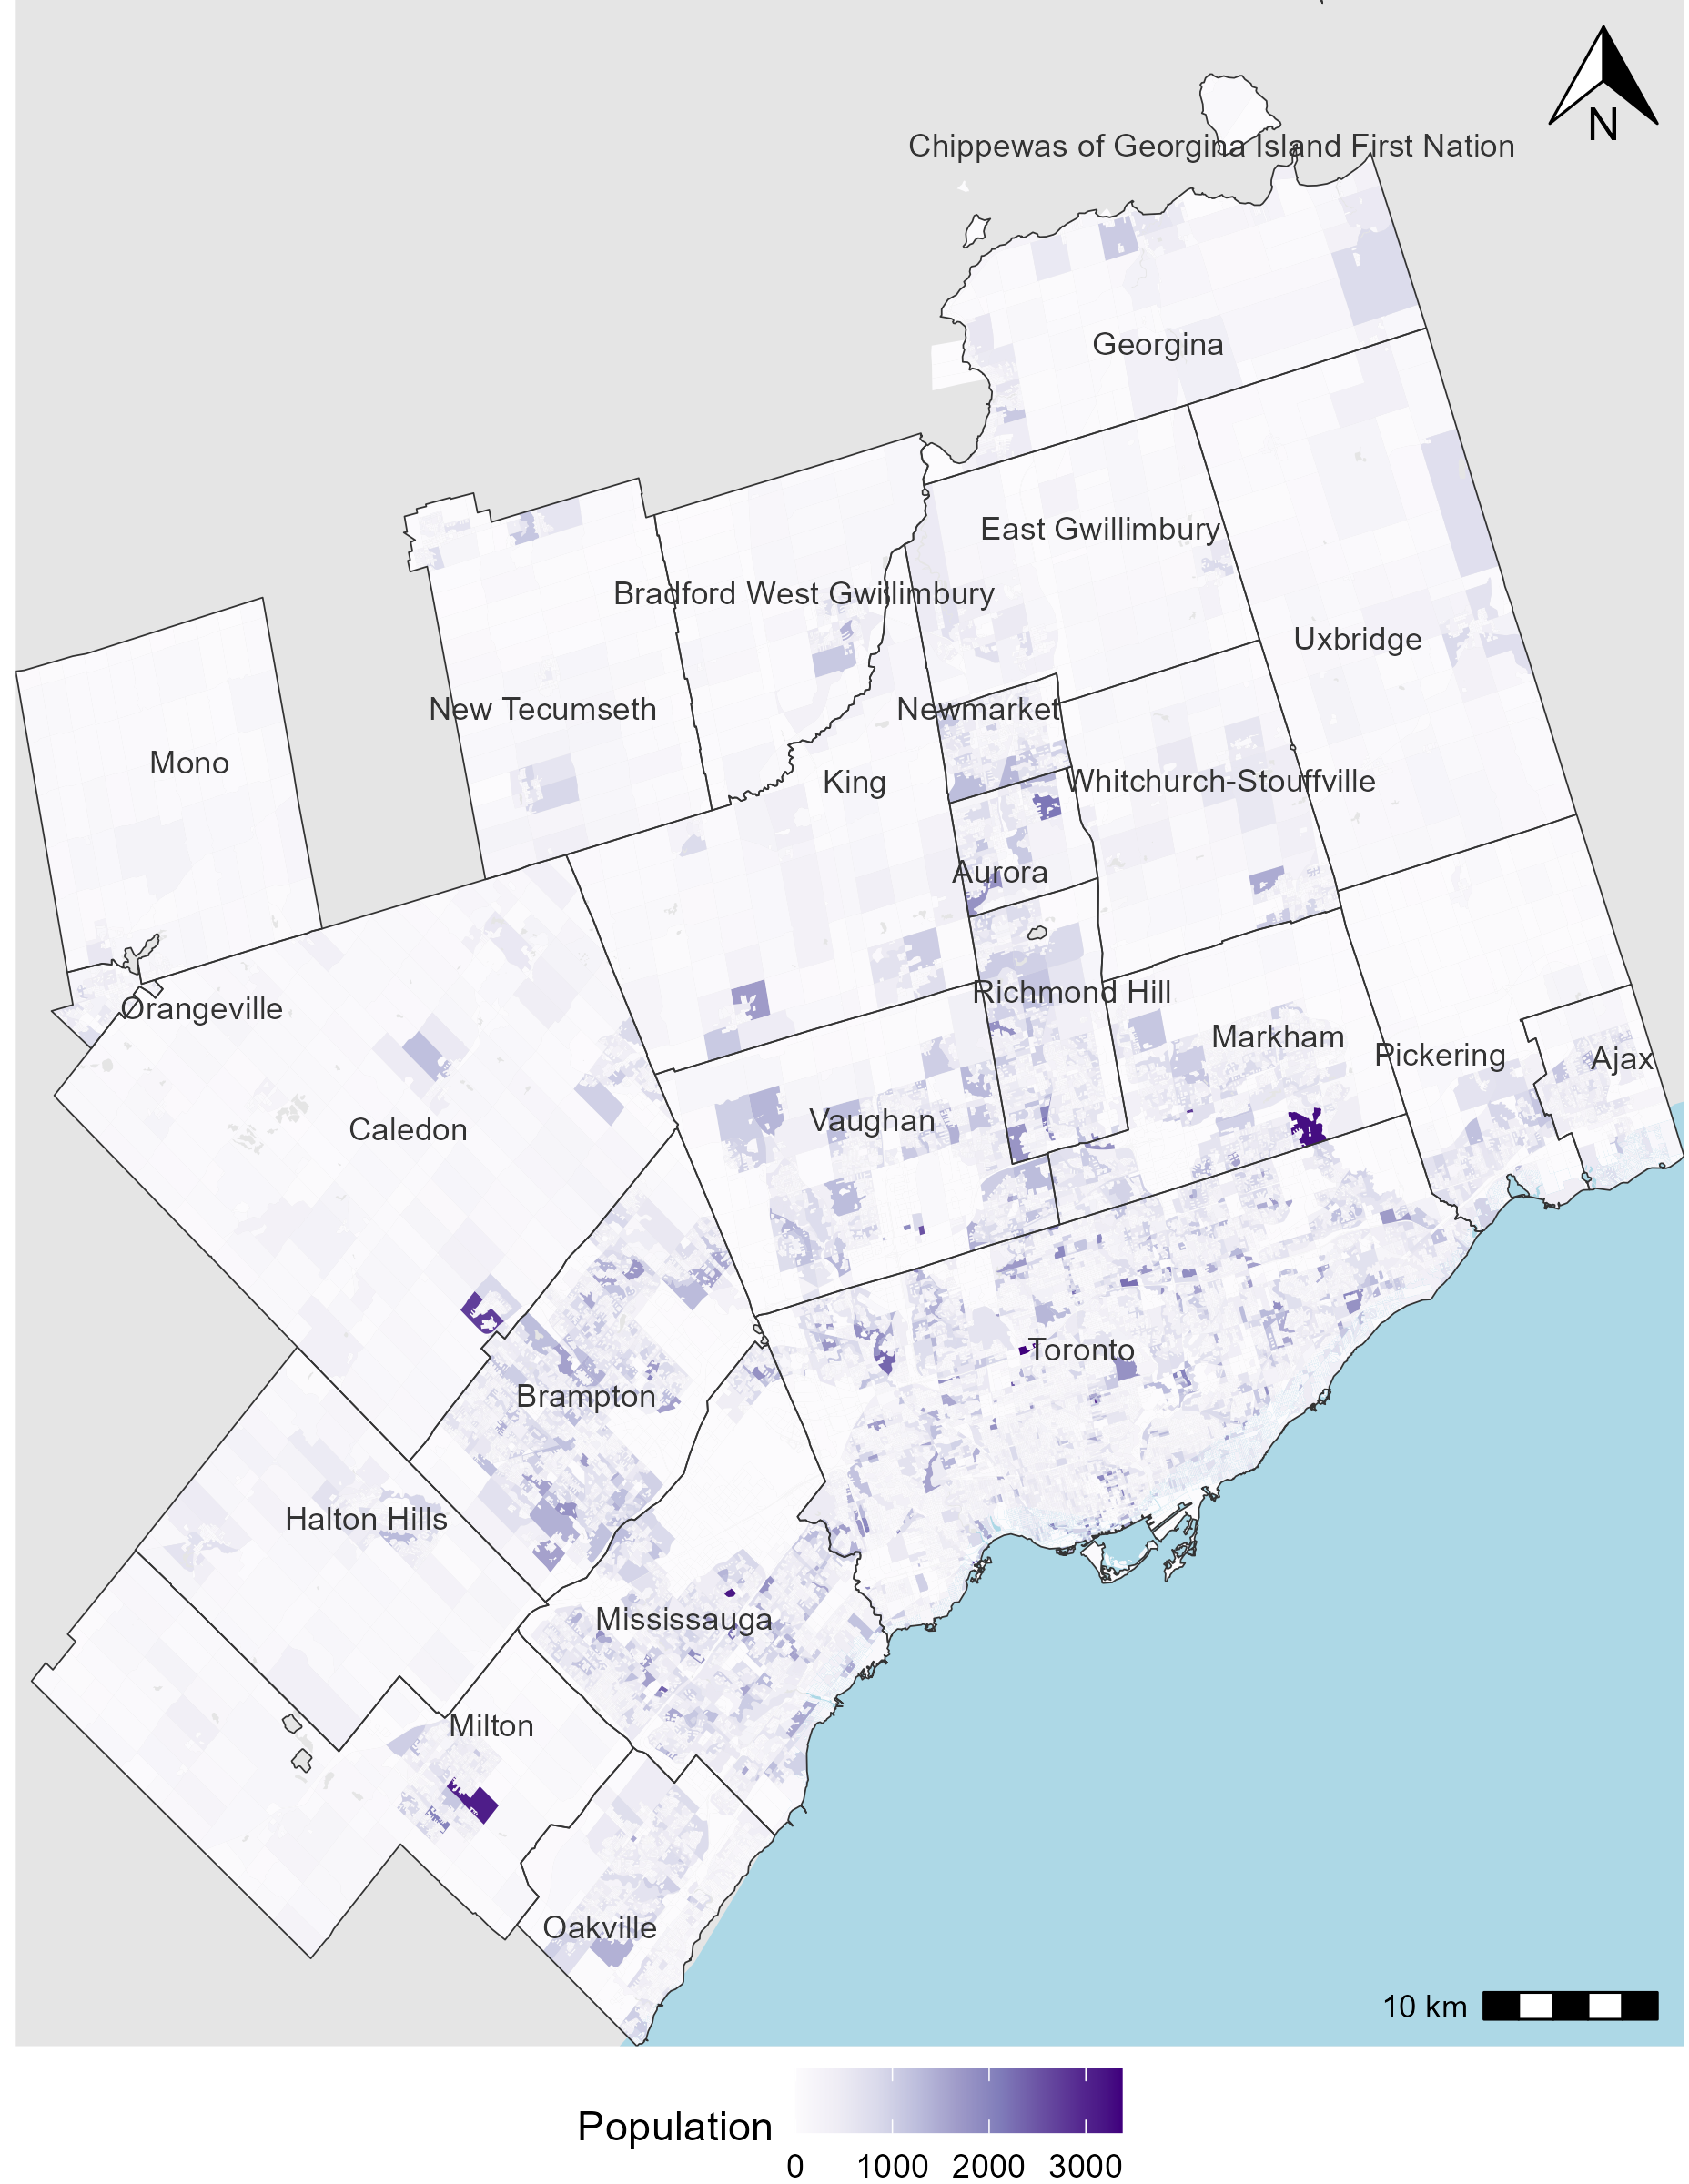
\includegraphics[width=6in]{./data/figures/chp3-toronto_CMA_plot} 

}

\caption{\label{fig:chp3-toronto_CMA_plot}Map of Toronto CMA with population per DB from the 2021 Census}\label{fig:unnamed-chunk-42}
\end{figure}

Two other important zoning systems for the city of Toronto are worth including. First, the city's former municipal boundaries. The modern City of Toronto is an amalgamation of six former municipalities. These boundaries, along with their names, are shown in Figure~\ref{fig:chp3-former_muni_boundaries_plot}, overlaid on DB-level population density.

Another commonly used zoning system, offering a slightly coarser spatial resolution, is the neighbourhood. Toronto contains 158 neighbourhoods, defined by the City staff for planning purposes. These are illustrated in Figure~\ref{fig:chp3-toronto_popden_NIAs_plot}. In addition to their geographic boundaries, neighbourhoods have also received a classification by the city, occasionally used for policy or program initiatives. This classification includes either: a ``Neighbourhood Improvement Area'' (NIA) (33 neighbourhoods), an ``Emerging Neighbourhood'' (EA) (10 neighbourhoods), or neither (the remaining 115 neighbourhoods). These classifications are based on a composite index developed by the City, incorporating indicators of population marginalization and neighbourhood infrastructure. The index includes factors such as economic opportunity (e.g., unemployment rates), social development (e.g., high school graduation rates), civic participation (e.g., voter turnout), infrastructure (e.g., walkability, availability of community spaces), and health outcomes (e.g., premature mortality) (City of Toronto, 2014, 2024). Overall, between both plots, it is notable that higher residential density is concentrated near the lake in Toronto's downtown core. Most NIAs are found in the eastern and northwestern parts of the city, and tend to have lower population densities---though a few high-density NIAs also exist downtown.

\begin{figure}

{\centering 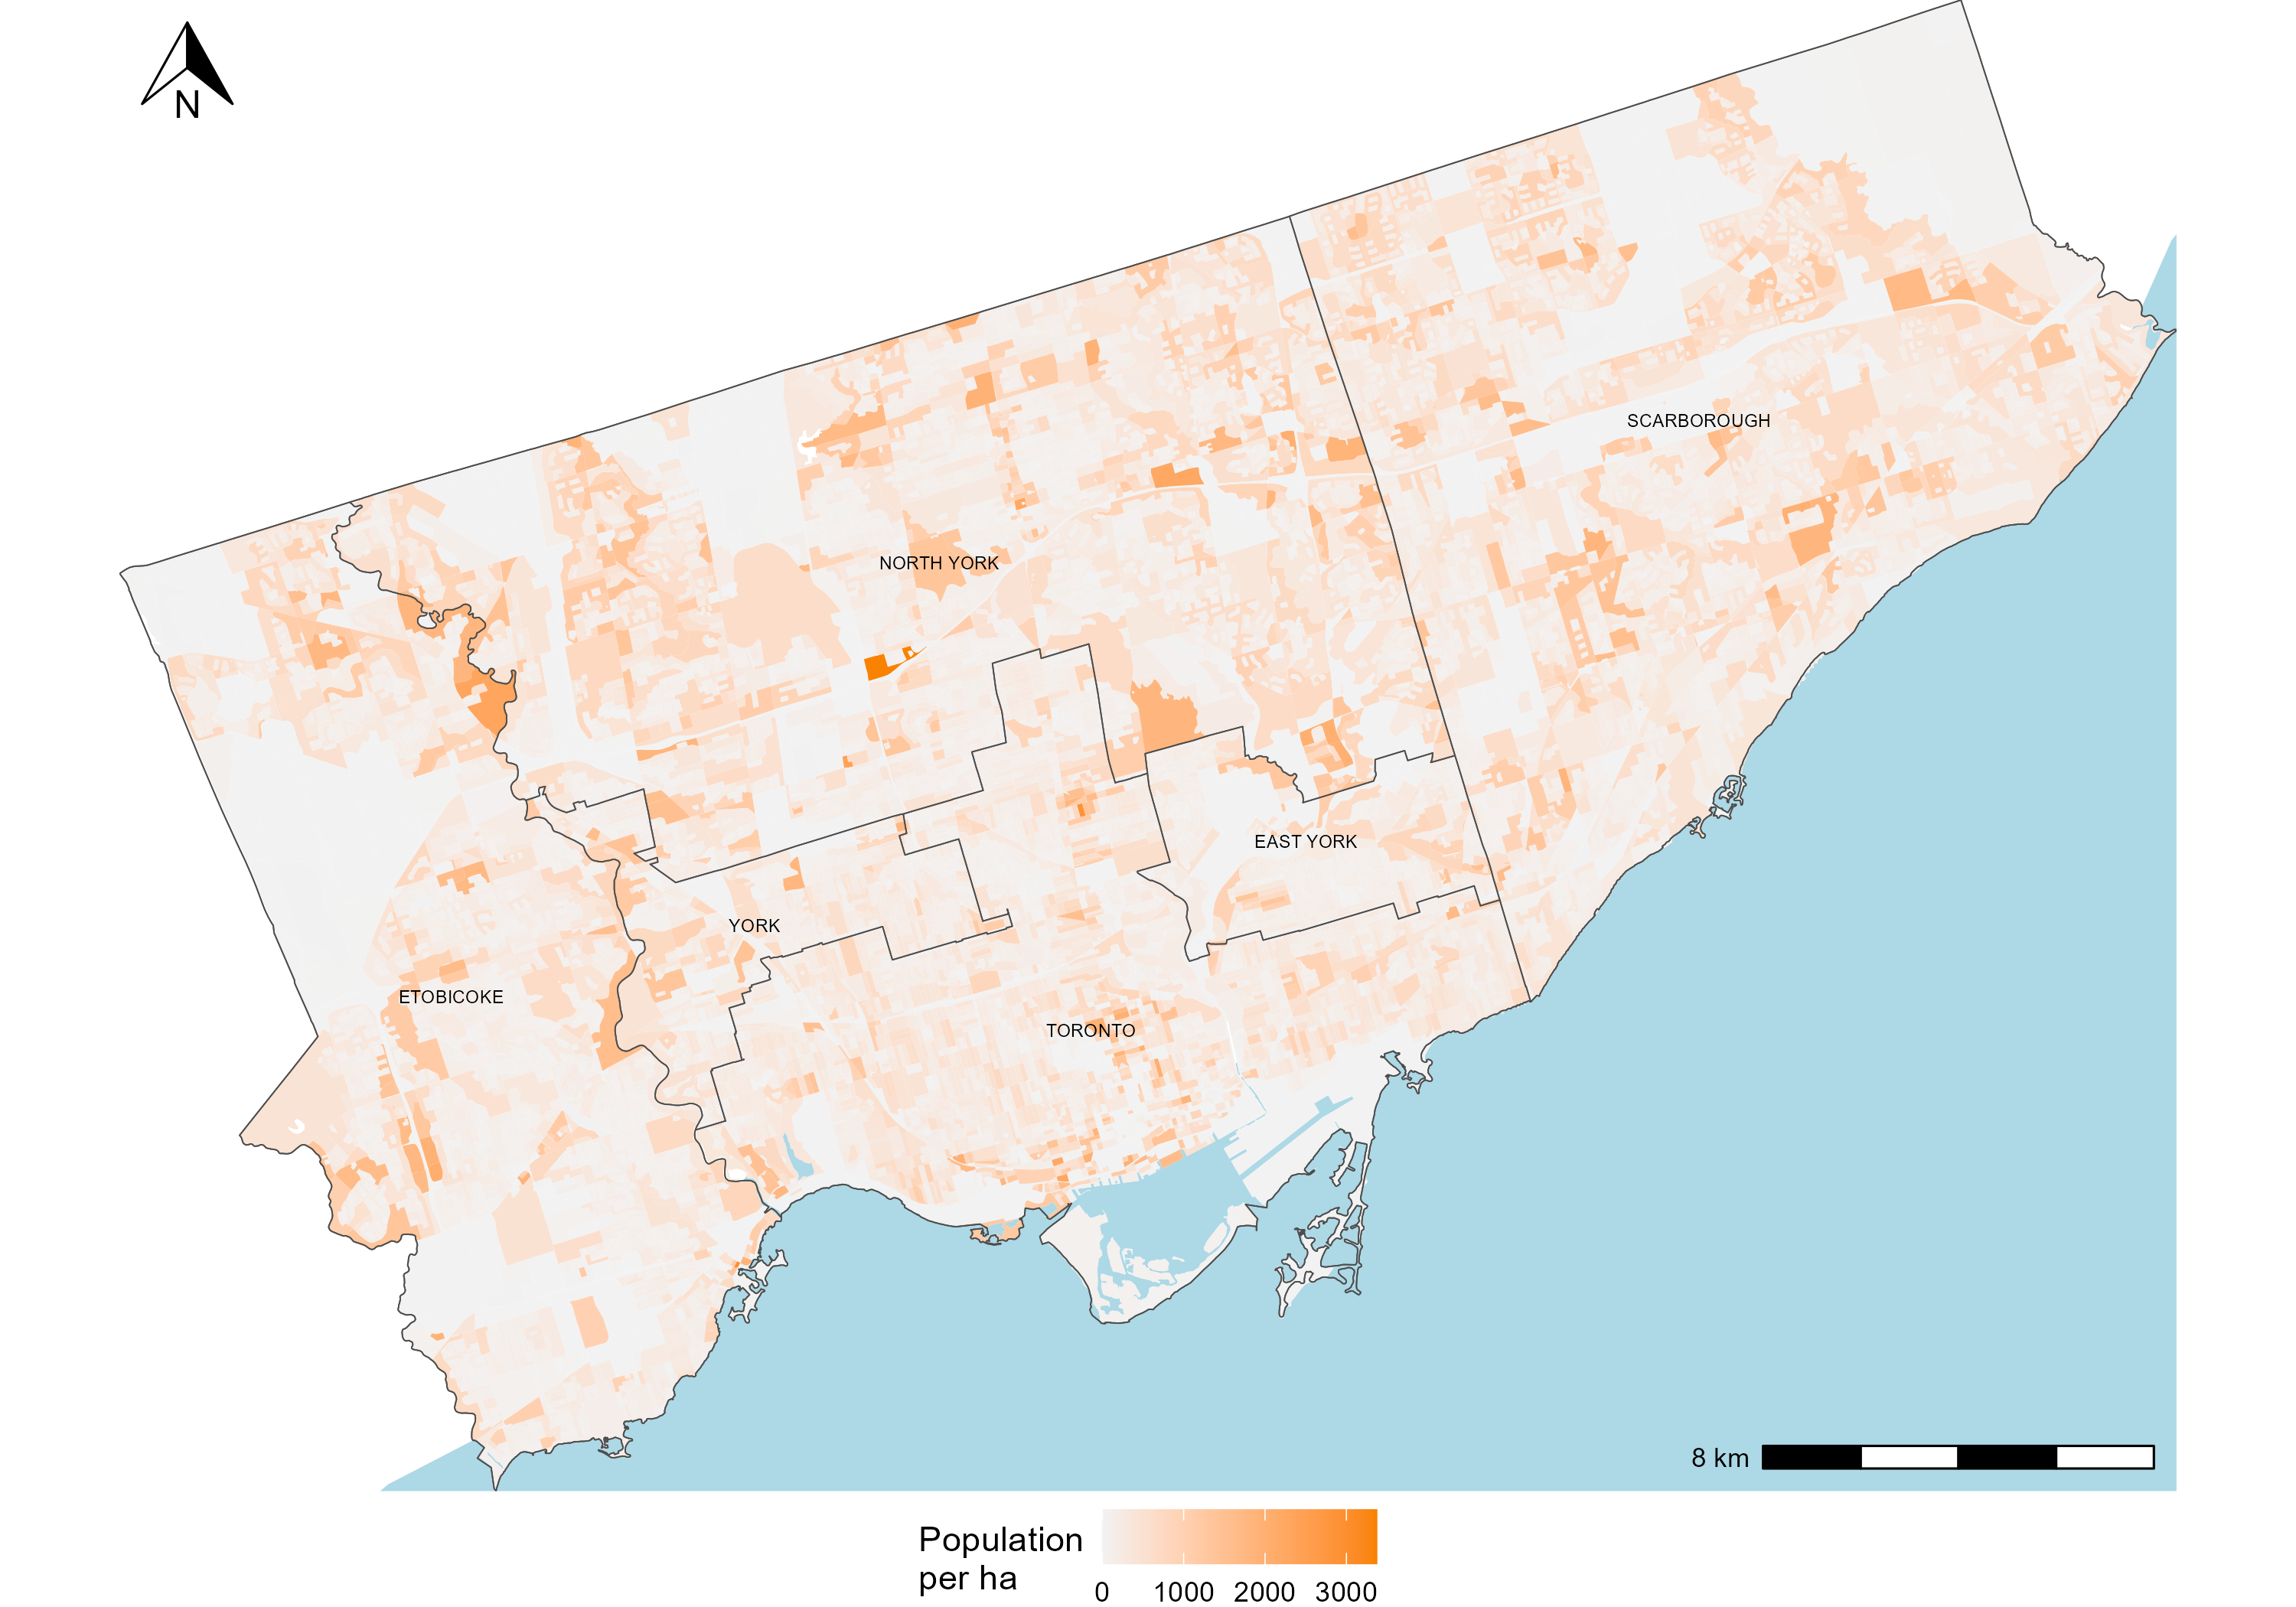
\includegraphics[width=6in]{./data/figures/chp3-former_muni_boundaries_plot} 

}

\caption{\label{fig:chp3-former_muni_boundaries_plot}Map of the City of Toronto's former municipal boundaries atop DB level population from the 2021 census}\label{fig:unnamed-chunk-43}
\end{figure}

\begin{figure}

{\centering 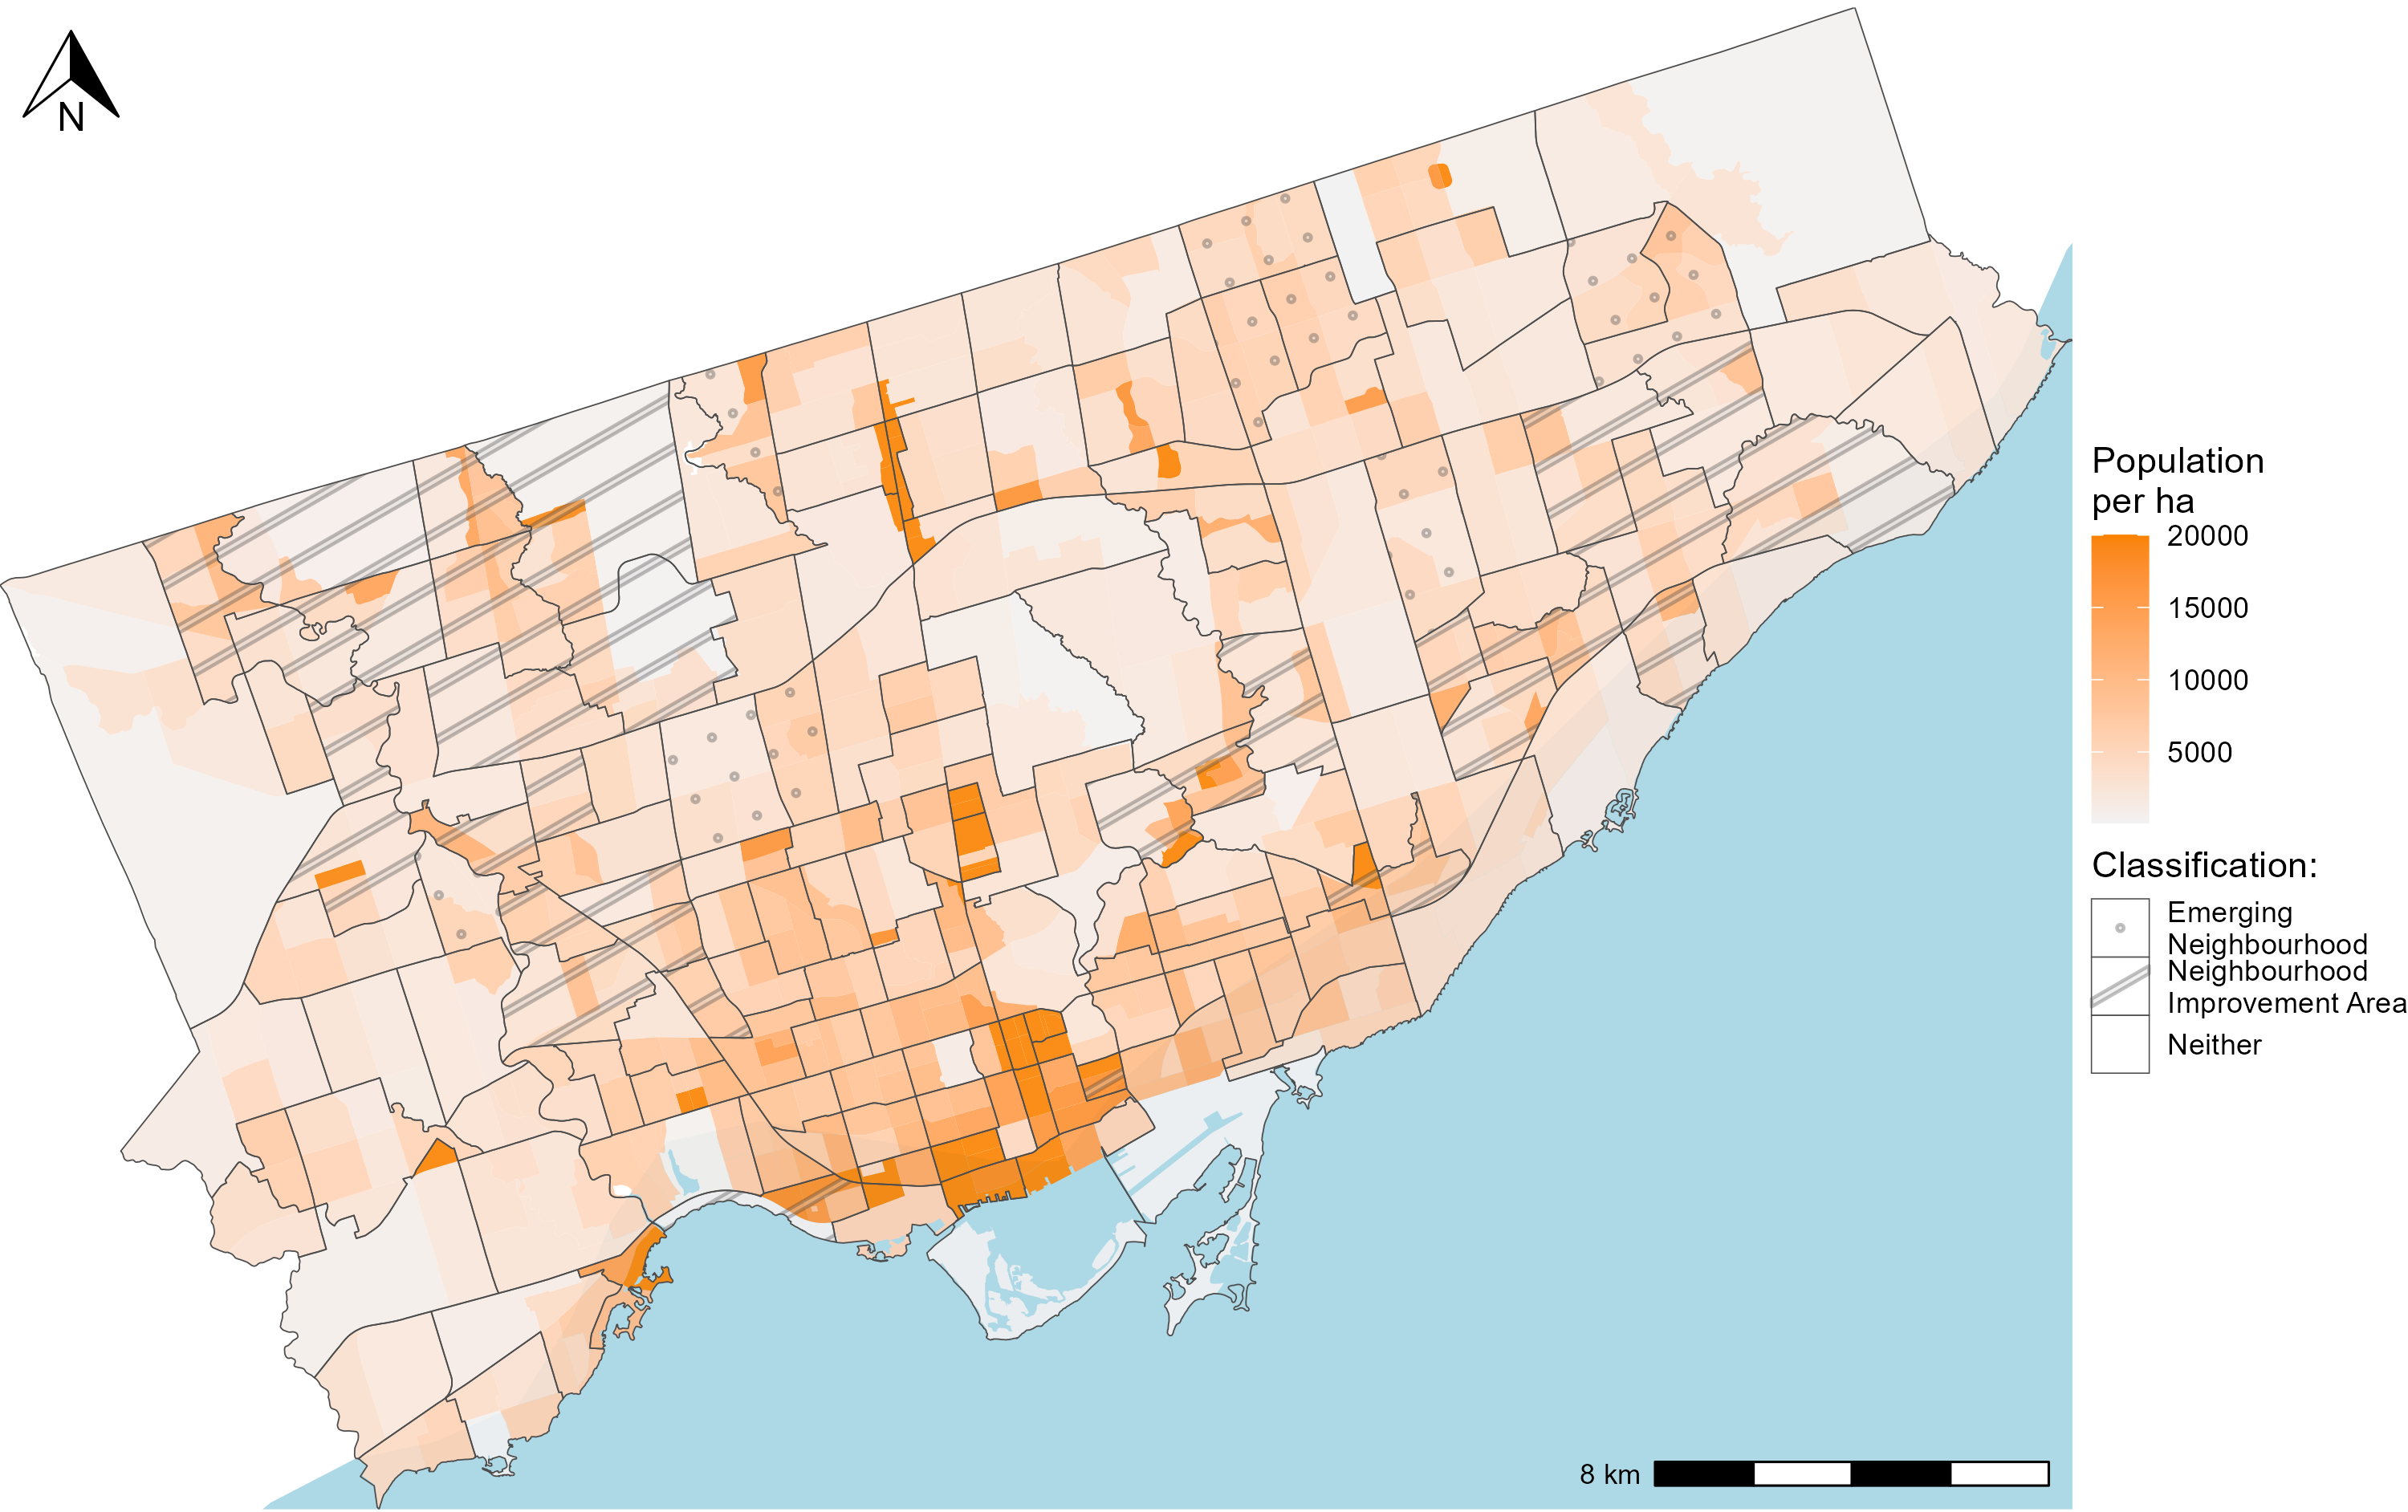
\includegraphics[width=6in]{./data/figures/chp3-toronto_popden_NIAs_plot} 

}

\caption{\label{fig:chp3-toronto_popden_NIAs_plot}Map of the 158 Toronto neighbourhoods, with 'Improvement' classification and population density from the 2021 Census}\label{fig:unnamed-chunk-44}
\end{figure}

And lastly, the Figure \ref{fig:chp3-toronto_popden_DBCent_plot} displays the calculated DB population-weighted centroids, used as the representative points of the origins in the accessibility analysis. There are 13322 points within the City, with a spatial clustering in parts of the city with higher population density (i.e., downtown).

\begin{figure}

{\centering 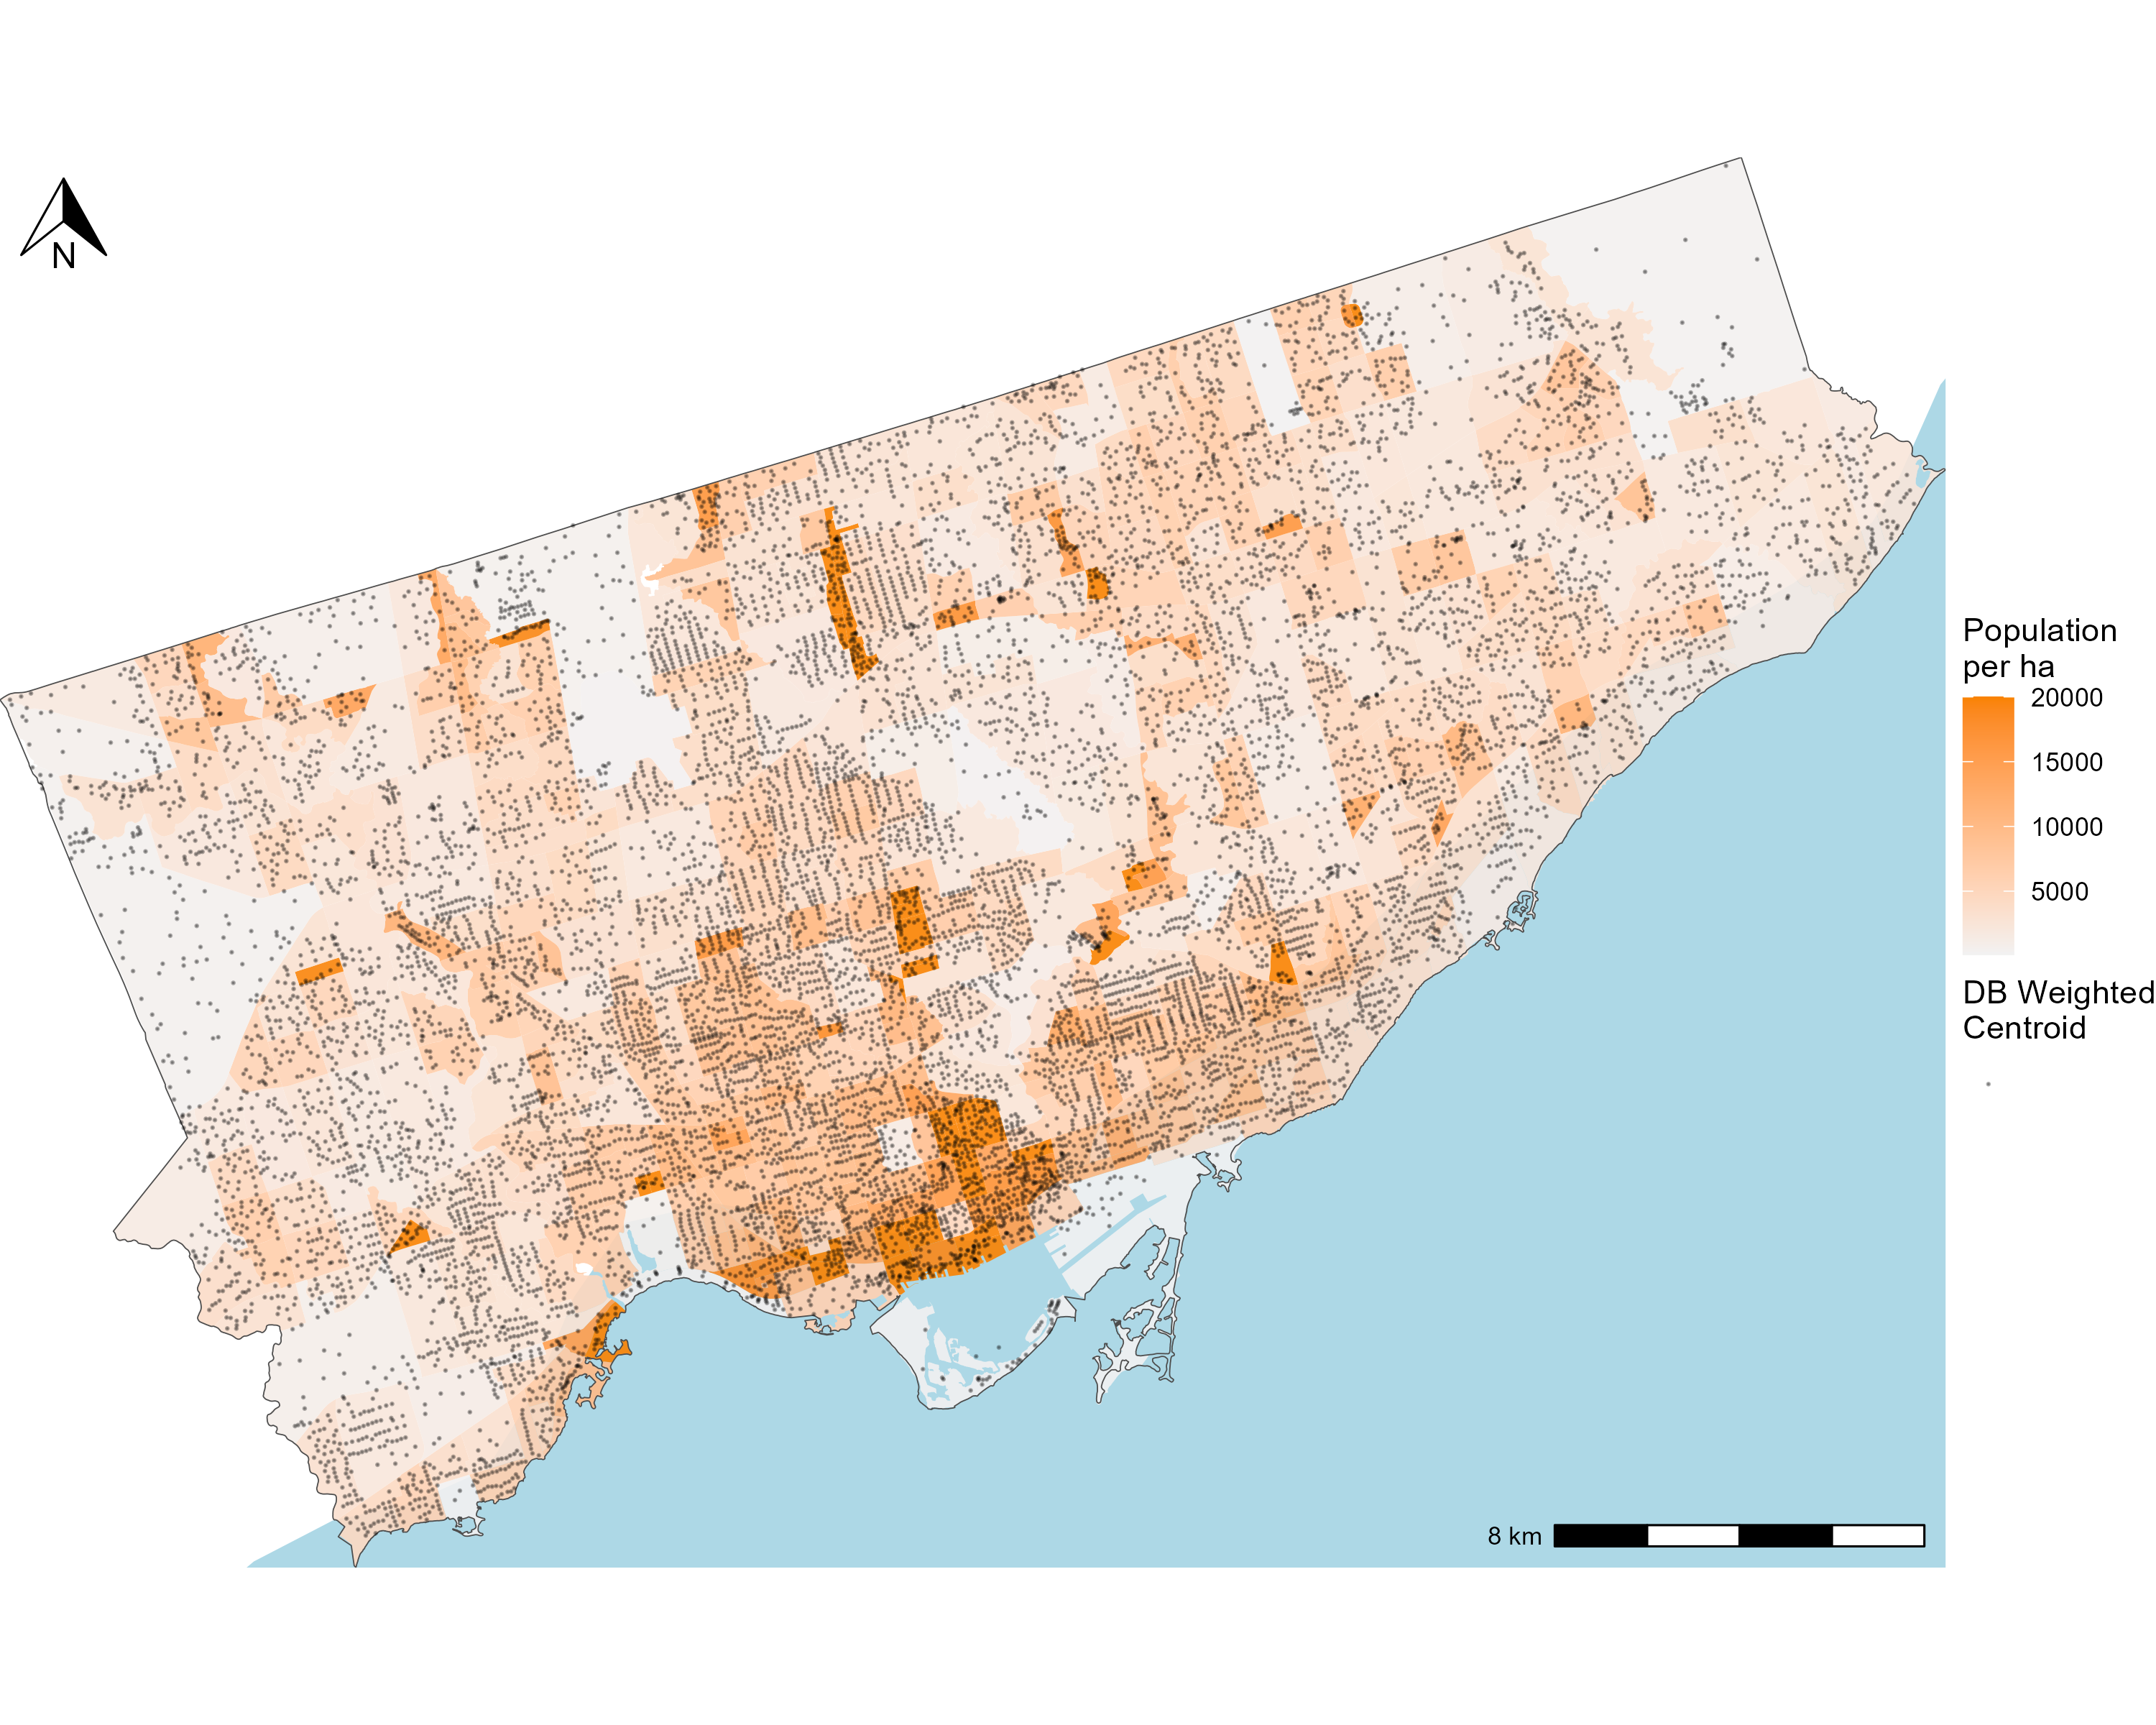
\includegraphics[width=6in]{./data/figures/chp3-toronto_popden_DBCent_plot} 

}

\caption{\label{fig:chp3-toronto_popden_DBCent_plot}Map of the City of Toronto's DB weighted centroids atop the population density from the 2021 Census}\label{fig:unnamed-chunk-45}
\end{figure}

\subsection{Toronto parkland destinations and normative travel behaviour}\label{toronto-parkland-destinations-and-normative-travel-behaviour}

Parkland is defined as city operated and/or owned `parks' identified in the greenspaces shapefile available through the city's official Open Data portal (City of Toronto, 2025). These are the same park assets that are identified as part of the Parkland Strategy report commissioned by the City of Toronto (City of Toronto, 2019, p. 20). This report serves as a guideline for assumptions made regarding park classification and interaction catchments based on park classification. Toronto's parkland is visualized in Figure \ref{fig:chp3-parkland_paths_plot}. Of note, other Open Spaces include in the greenspaces shapefile are federally or provincially owned/operated spaces, school yards, cemeteries, and hydro corridors. These spaces are not assumed to be Toronto operated and/or owned parkland, hence are not included in this analysis. These greenspaces are reflected as `no population' DBs.

\begin{figure}

{\centering 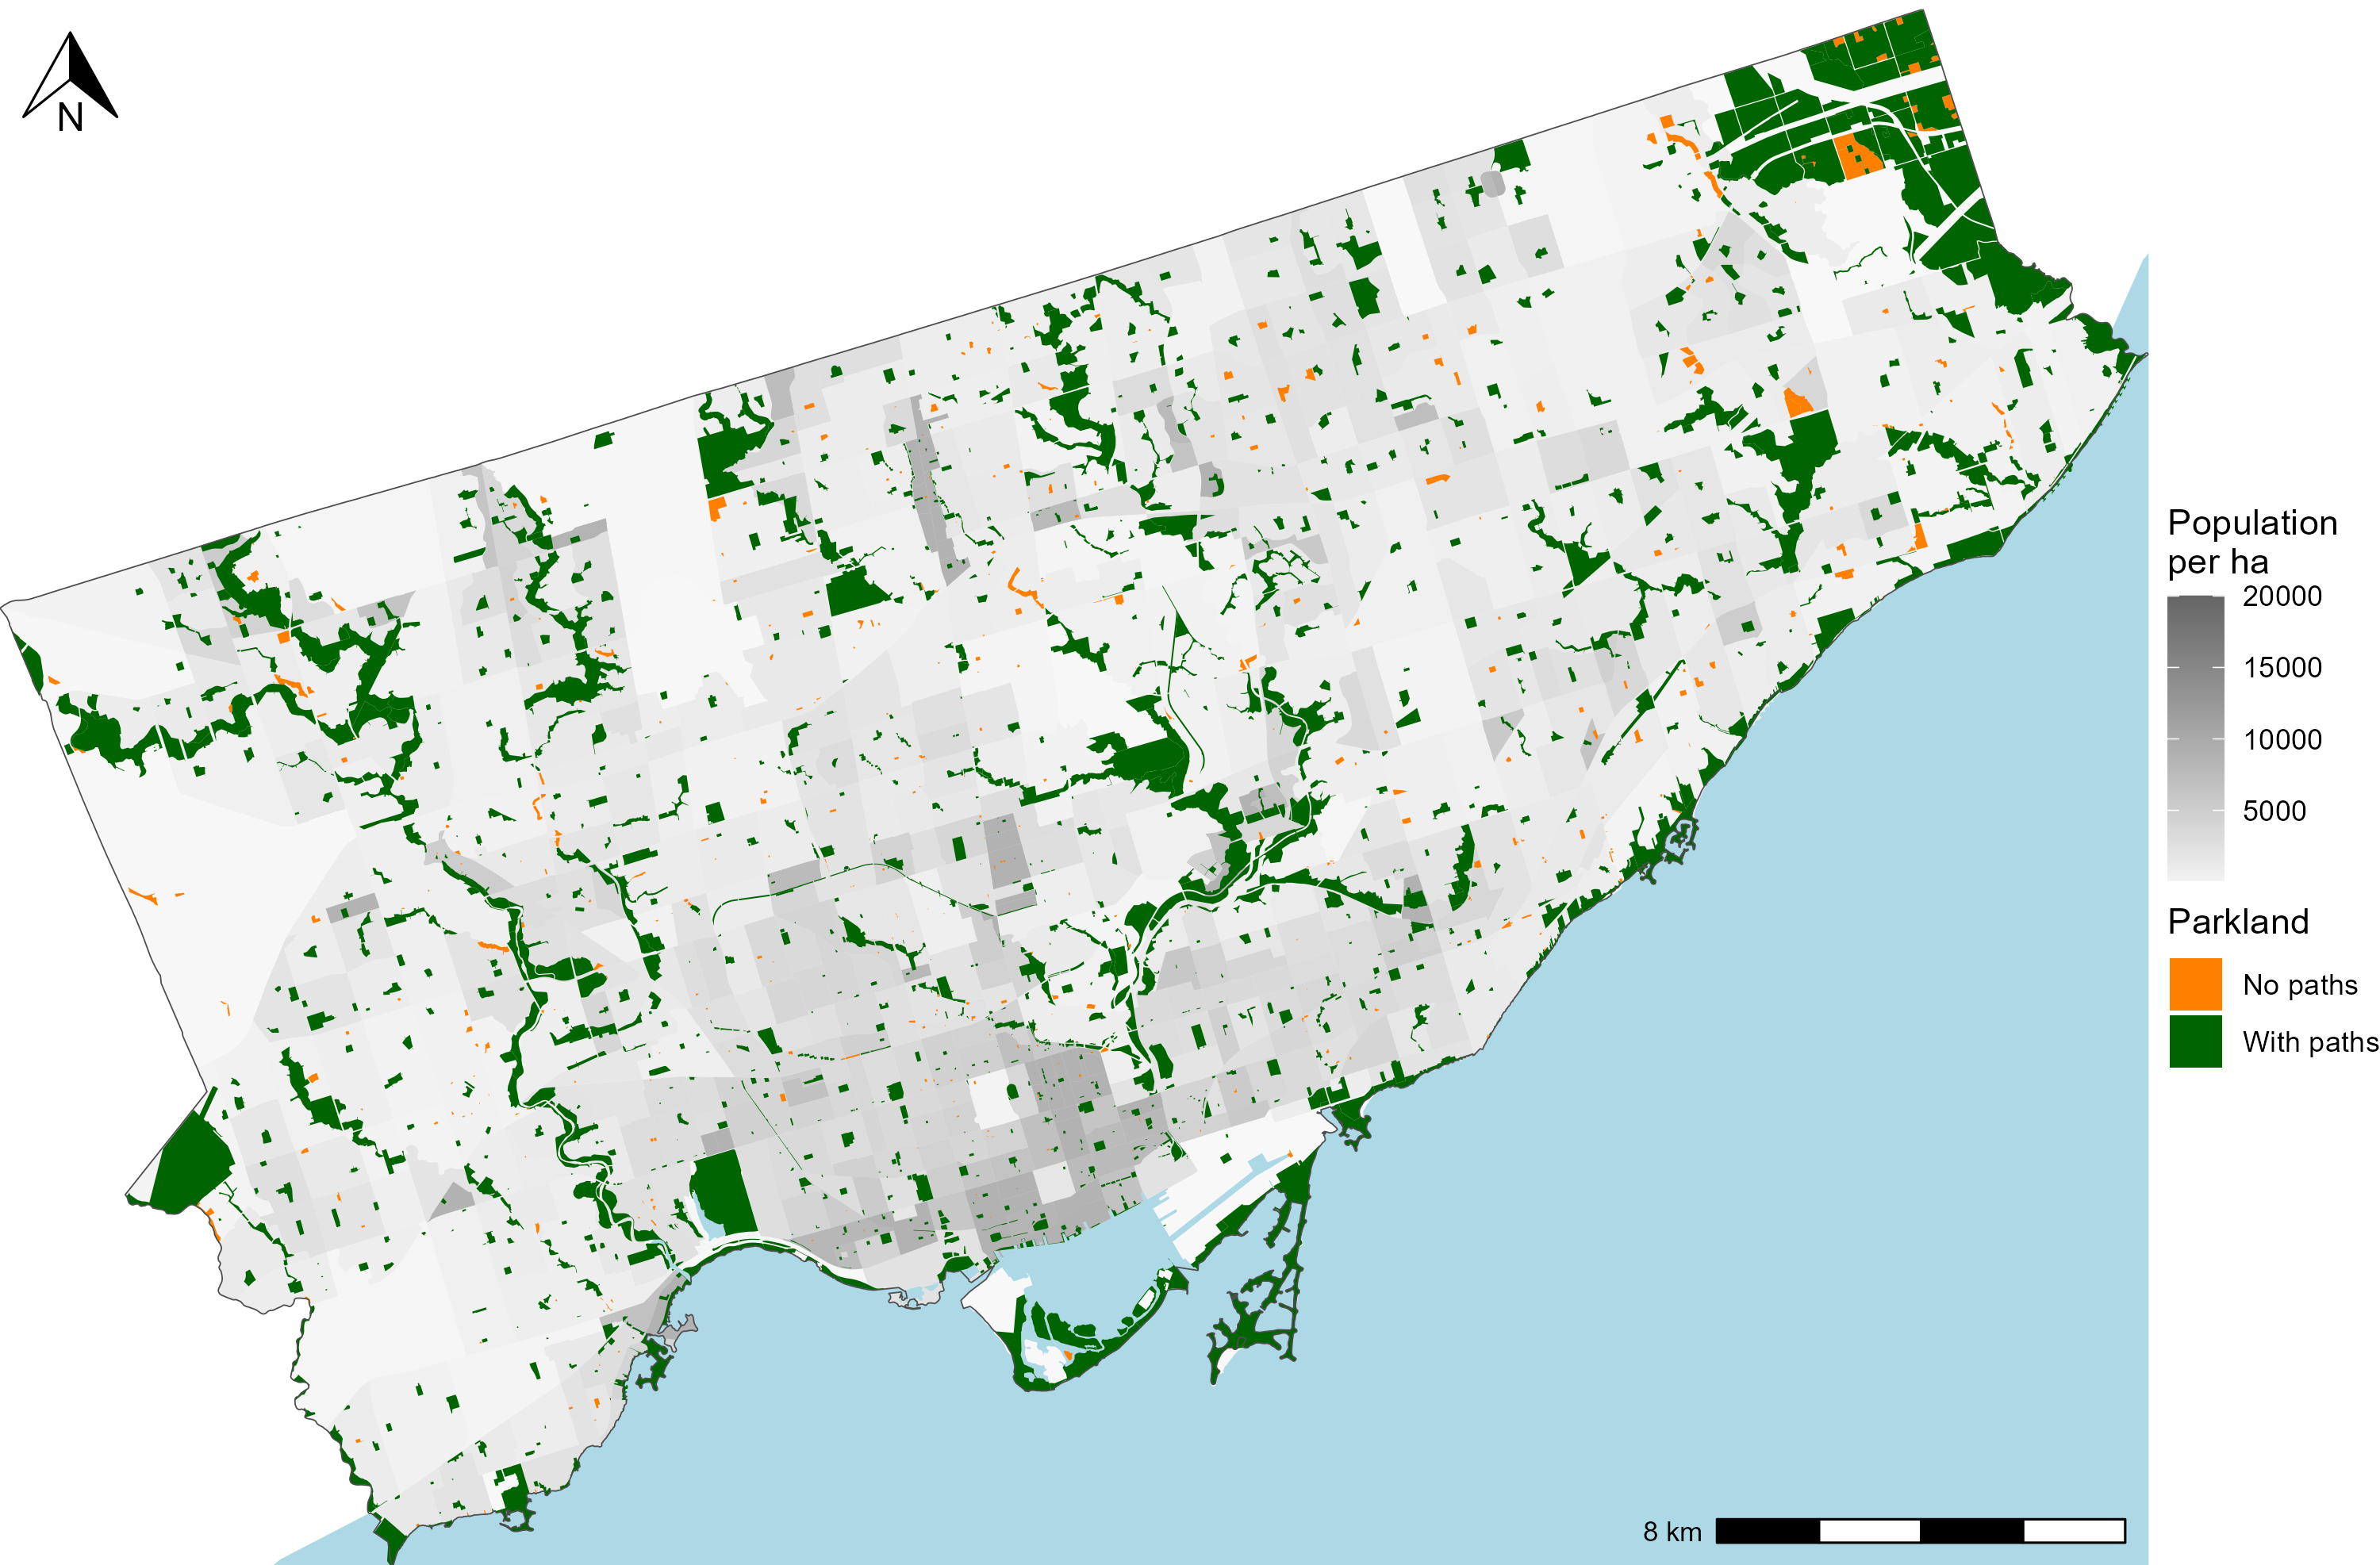
\includegraphics[width=6in]{./data/figures/chp3-parkland_paths_plot} 

}

\caption{\label{fig:chp3-parkland_paths_plot}Map of the City of Toronto's Parkland (with paths or no paths) atop the population density from the 2021 Census}\label{fig:unnamed-chunk-46}
\end{figure}

As retrieved from City of Toronto (2019, p. pg.15), the parkland can be categorized by size: `Parkette' (\textless0.5 ha) (40\% of all parks), `Small Park' (0.5--1.5 ha) (20\%), `Medium Park' (1.5--3.0 ha) 16\%, `Large Park' (3.0--5.0 ha) 9\%, `City Park' (5.0--8.0 ha) 5\%, and `Legacy Park' (\textgreater8.0 ha) 10\%. Interaction with parks can be assumed in a variety of ways, but in this analysis, it is normatively (A. Paez et al., 2012) defined based on the park classification catchments described in City of Toronto (2019) as well as assumptions associated with the mode: as outlined in the following section.

How parks can potentially be accessed is assumed based on their entrances. Entrances are not explicitly available, so they are assumed. They are calculated based on the parkland edge intersection with each path within the park itself or intersecting the park edge. 4 of the the 1607 parks have paths, each with anywhere between 1 to 84 (median of 2) entrances. The remaining 1603 parks do not have paths, and hence their entrances cannot be precisely assumed. Parks without an entrance are significantly smaller in area (i.e., median of 0.24 ha as opposed to the median of area parks with paths which is 1.43 ha). Upon visual inspection using Google Maps streetview, parks with no paths often contain a playground, some sport amenity or gardens within the center. Some of them are unfurnished -containing only mowed grass. For these parks with no internal paths, it is assumed then that these spaces can be entered from any direction and that the geometry centroid is the point of interest calculated and assumed as the entrance point. This point is snapped onto the transportation network based on an origin's shortest path, as will be later described in the routing subsection.

As a visualisation, Figure \ref{fig:chp3-park_entrance_example_plot} contains a panel of three DAs in Toronto, each displaying the roads, parks, and assumed park entrances. Readers should note that in the first two panels, these parks contain multiple entrance points, corresponding to where the edge of the paths within the parks intersect with the edge of the park boundary. These plots showcase different DAs that represent the diversity in DA size and park composition across the city. The first plot showcases a relatively small DA, near the downtown core of the city featuring high density of population, other amenities and multimodal transportation systems. This DA is unique in the area, as it features a large planned `Legacy' park by the name of Christie Pits. Planned parks are typically square or rectangular and can be accessed from most of the sides. They are also contained within the city in all areal sizes. The second plot contains a larger DA, north of downtown, that contains a few parks and near higher density suburban built form. One is the Roycroft Park Lands, a large `City' (smaller than Legacy), part of the Don River wetlands with maintained trails, enjoyed as nature reserve. Note its long shape and minimal number of entrances. Natural parklands like Roycroft Park Lands are common along wetlands and other preserved natural spaces; they are typically larger in size (Medium, Large, or City parks) hence offer a lot of parkland space to those near their entrances. In the third plot, the DA is also large but with lower density suburban built form, and mostly residential. It contains only one small park: Pleasantview Park. This park contains no internal pathways, a playground in the middle of the park with no other amenities.

\begin{figure}

{\centering 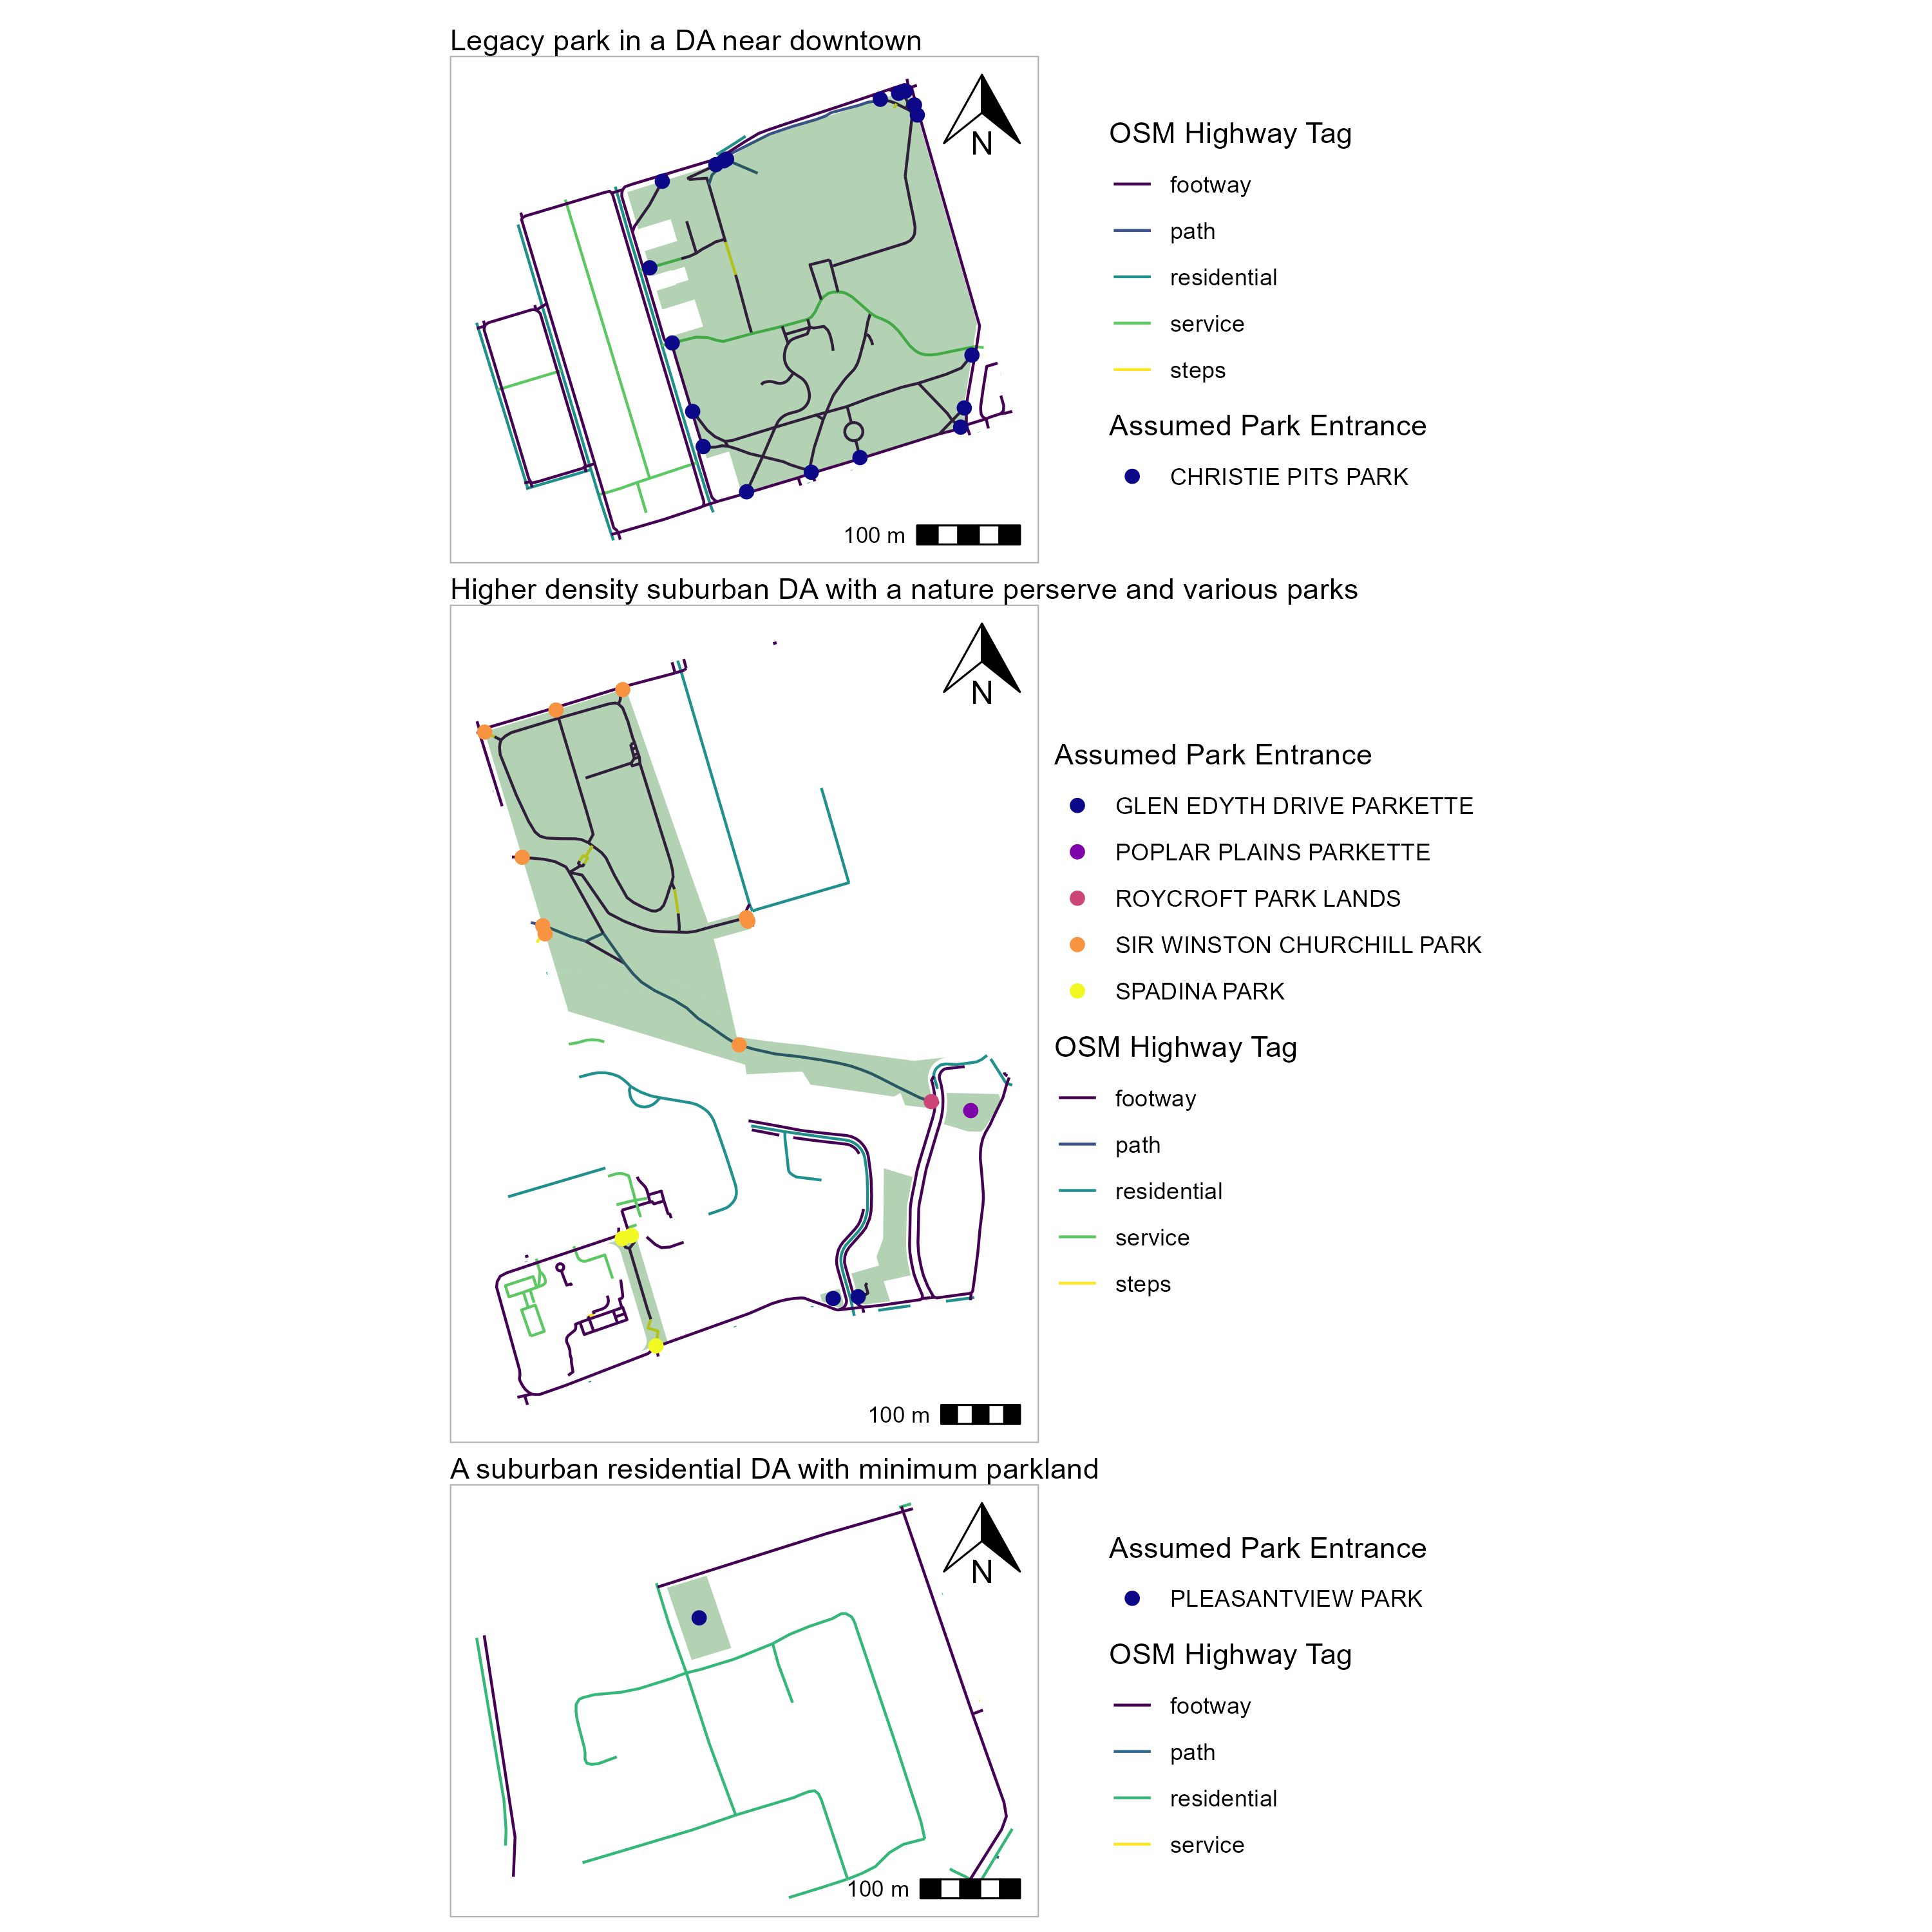
\includegraphics[width=6in]{./data/figures/chp3-park_entrance_example_plot} 

}

\caption{\label{fig:chp3-park_entrance_example_plot} Three DAs featuring parkland, road network by OSM tag, and park entrances. From top to bottom: planned Legacy park Christie Pits near the downtown core, parks north of the downtown core preserving natural space, and planned park with no paths in a more suburban DA.}\label{fig:unnamed-chunk-47}
\end{figure}

\subsection{Origin to destination routing and trip lengths}\label{origin-to-destination-routing-and-trip-lengths}

Routing of travel times was done using the travel\_time\_matrix() function in \{r5r\}, an R package that provides an R-interface for the Java-based R5 Routing engine (R. H. M. Pereira, Saraiva, Herszenhut, Braga, \& Conway, 2021). The function was run four time, one for bicycle, car, transit and walking modes, producing four separate travel time matrices. Each origin destination pair has an associated shortest travel time, selected by the function based on all possible origin destination routes given the input road network (and transit schedule, for the transit mode). The road network is an edited version of OpenStreetMaps (OSM) street network (December 9, 2022) and edited General Transit Feed Specification (GTFS) files (February 4, 2024) for transit operating within the City i.e., GO (regional commuter train and bus service), TTC (local subway, lightrail, and bus network), and the UP Express (regional commuter train line). The files were edited by city staff to more accurately reflect access into TTC subway stations and reflect the transit schedule for the week of February 4 2025.

Concerning the inputs for the `travel\_time\_matrix()' function for all modal travel time calculations: the origins are the DB weighted centroids (13322 locations), the destinations are points representing the 1607 parks and the OSM road network were used. Some parks have multiple pieces, separated by the road network: in total, there are 1958 park pieces, each with between 1 and 68 path entrances (median 3 entrances) or 1 park piece centroid. In total, there are 6274 possible destination points (5724 path entrances and 550 centroids) for each of the 13322 origins.

For the motorized modes, a maximum travel time of 120 minutes was selected. For transit, the GTFS files and a departure time of between 11:00-11:15am (i.e., a 15 minute departure window) on February 8th 2025 was used, to reflect a Saturday afternoon transit schedule. Travel speeds reflect the posted speeds and intersections as gleaned from the OSM road network, and for transit, the scheduled transit arrival times at stops according to the GTFS file. For non-motorized modes, a maximum travel time of 30 minutes was selected, and the default travel speeds of 3.6 km/h for walk and 12 km/h for cycling was assumed. The travel time thresholds of 120 minutes and 30 minutes was set to normatively reflect the likelihood to travel to parks, by mode.

It is worthwhile summarising the multimodal travel time matrices. Notably, within a 120 minutes trip by motorized modes, the majority of DBs can reach all parks by car (with exception to the 6 on the Toronto Islands, inaccessible by car), i.e., the median DB can reach 1601 out of the 1607 parks, while the most isolated can still reach 184 parks. By contrast, within a 120 minute trip or less by transit, a median DB can only reach 1116 parks, with the most central DB reaching 1539 parks meaning 4\% of parks are feasibly unreachable by transit for DBs in the City of Toronto. These parks are located at the edges of the city. Comparing this modal `reach' to the lower range non-motorized modes, the number of parks reachable by foot or by cycle within 30 minutes from a DB is much lower: a median DB can only reach 15 parks (max. 61 parks for the most central DB) by walking and 86 parks (max. 295 parks for the most central DB) by cycling.

As a final note on routing assumptions, for all parks with assumed path entrances: it's useful to compare travel times to park centroids versus park path entrances to test the sensitivity of this assumption. For the 1204 parks with known path entrances, centroids were also computed and travel times from all DBs to all centroids were calculated. This comparison highlights the impact of the R5 routing algorithm, namely, how the routed travel times can differ depending on how the destination points are `snapped' to the nearest road segment.

If a park entrance point is not already on the transportation network, R5 snaps it to the nearest network segment, adding a walking time penalty based on distance. This snapping algorithm prioritizes minimizing overall travel time from the origin. Since edge entrances are typically already on the network, their snapping penalty is minimal. In contrast, centroid points--especially in large and irregular natural parks--may snap to parts of the road network that are unreachable by certain roads (e.g., far enough away from bus stops, or bike lanes), inflating travel times. Hence: when paths within the parks are available from the OSM network, they are used, as it more accurately reflects the points at each the parks can actually be entered from. But when the park has no entrances, it is assumed that the centroid (or the middle of the park itself) is the destination point, and the associated snapping penalty is folded into the calculated travel time. The following Figure \ref{fig:chp3-ent_vs_cent_tt_car_transit_scatter} and Figure \ref{fig:chp3-ent_vs_cent_tt_cycle_walk_scatter} demonstrate the relationship between the minimum travel time used in the analysis for each parks with path entrances and the travel time if its centroid point was used, along with a 45 degree dashed line representing a perfect linear relationship.

Regarding the motorized modes in Figure \ref{fig:chp3-ent_vs_cent_tt_car_transit_scatter}), the relationship appears to be roughly linear, with centroid times being consistently lower than path entrance times--except for a few parks that fall to the left of the dashed line. Parks with entrance times that are larger than their centroid times have entrances that are not in opportune positions on the network relative to the snapped centroid point, and vice versa for entrances that have \emph{lower} travel times than their centroid points which is often the case. Transit shows a similar trend but with more noise. A few parks exhibit exceptionally high transit times relative to their centroid times. These are typically larger parks where the centroid snaps to a location near access points to the transit system, but the \emph{actual} path entrances are not in proximity to those opportune system access point. Since the road network for cars is more continuous and the system is more evenly accessible (e.g., the majority of roads can be driven on, whereas the transit system can only be entered in specific points), this discrepancy is not observed in the car mode. This comparison underscores the importance of using realistic entrance points especially for larger parks with few entrance points and for modes like transit, which do not provide uniform access into the system.

\begin{figure}

{\centering 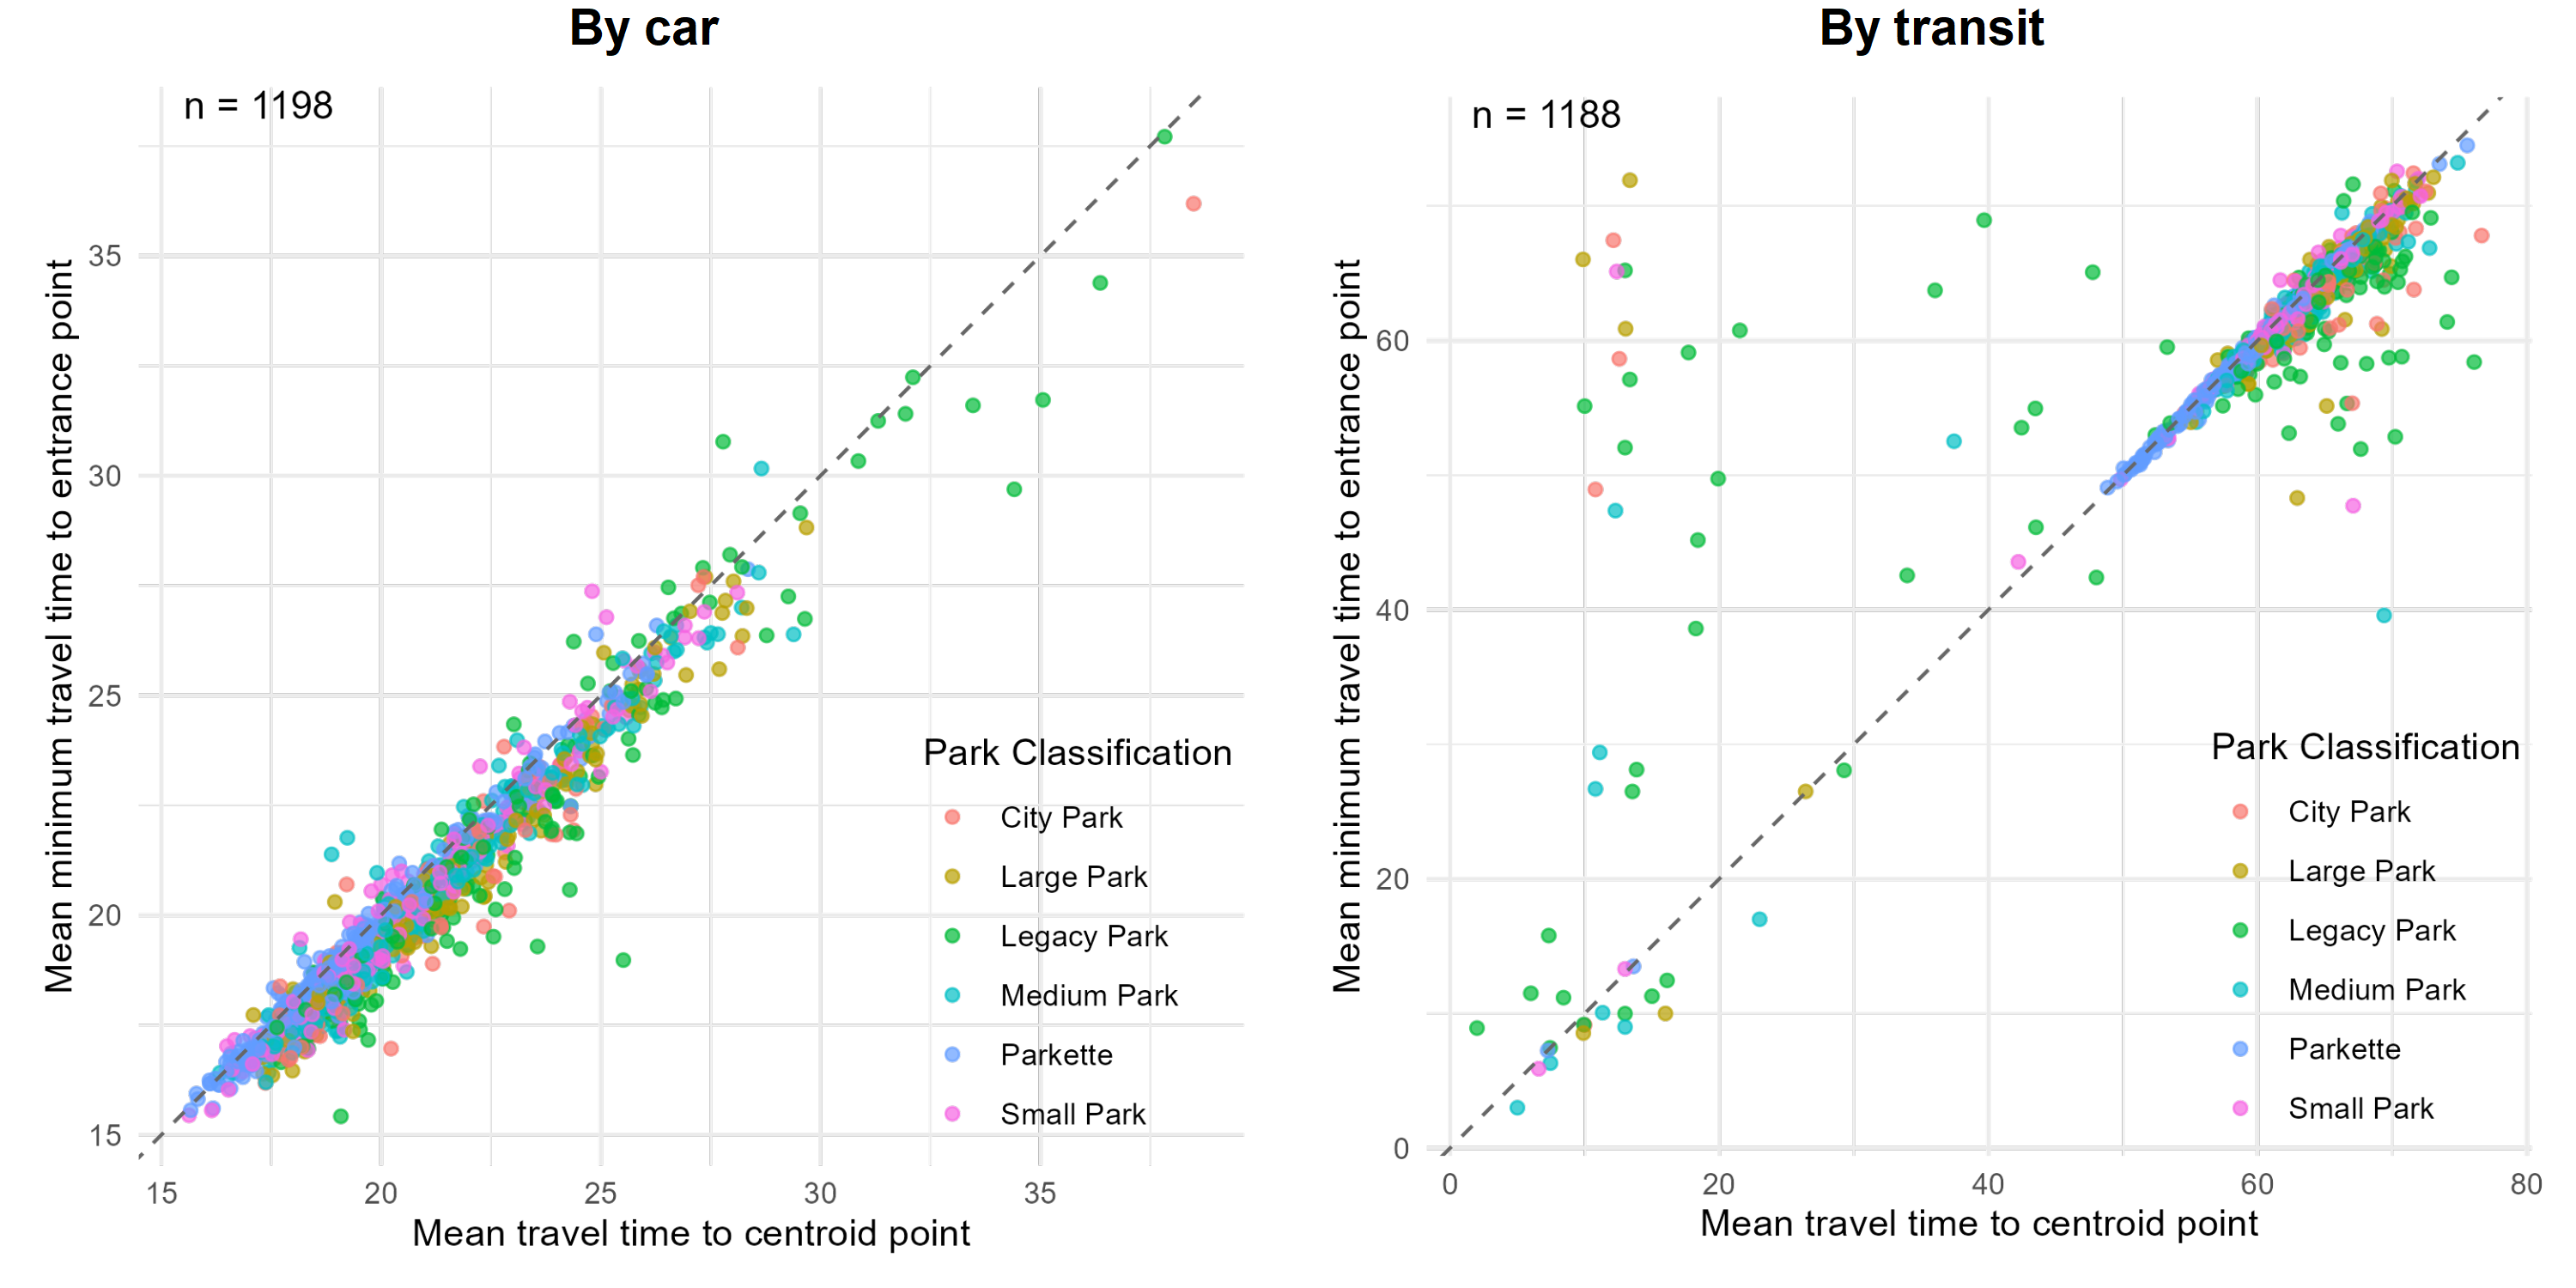
\includegraphics[width=6in]{./data/figures/chp3-ent_vs_cent_tt_transit_car_scatter} 

}

\caption{\label{fig:chp3-ent_vs_cent_tt_car_transit_scatter} Scatter plot of car and transit travel times from origins to destinations by destination type for each park (either mininum median travel time to park centroid, or minimum median travel time to park entrance). }\label{fig:unnamed-chunk-48}
\end{figure}

Figure \ref{fig:chp3-ent_vs_cent_tt_cycle_walk_scatter} captures the comparision between the non-motorized mode travel times, which exemplifies a similar pattern as the motorized modes. Namely, centroid travel times are typically longer than path entrance points in a linear relationship. However, unlike transit and car, travel by bike and walk demonstrate different levels of noise. As the travel time threshold is 30 minutes, distance can be traversed at a faster rate by bike than by foot, hence differences in distances between the path entrance point and the snapped centroid is less impact on the estimated travel time for bike mode.

\begin{figure}

{\centering 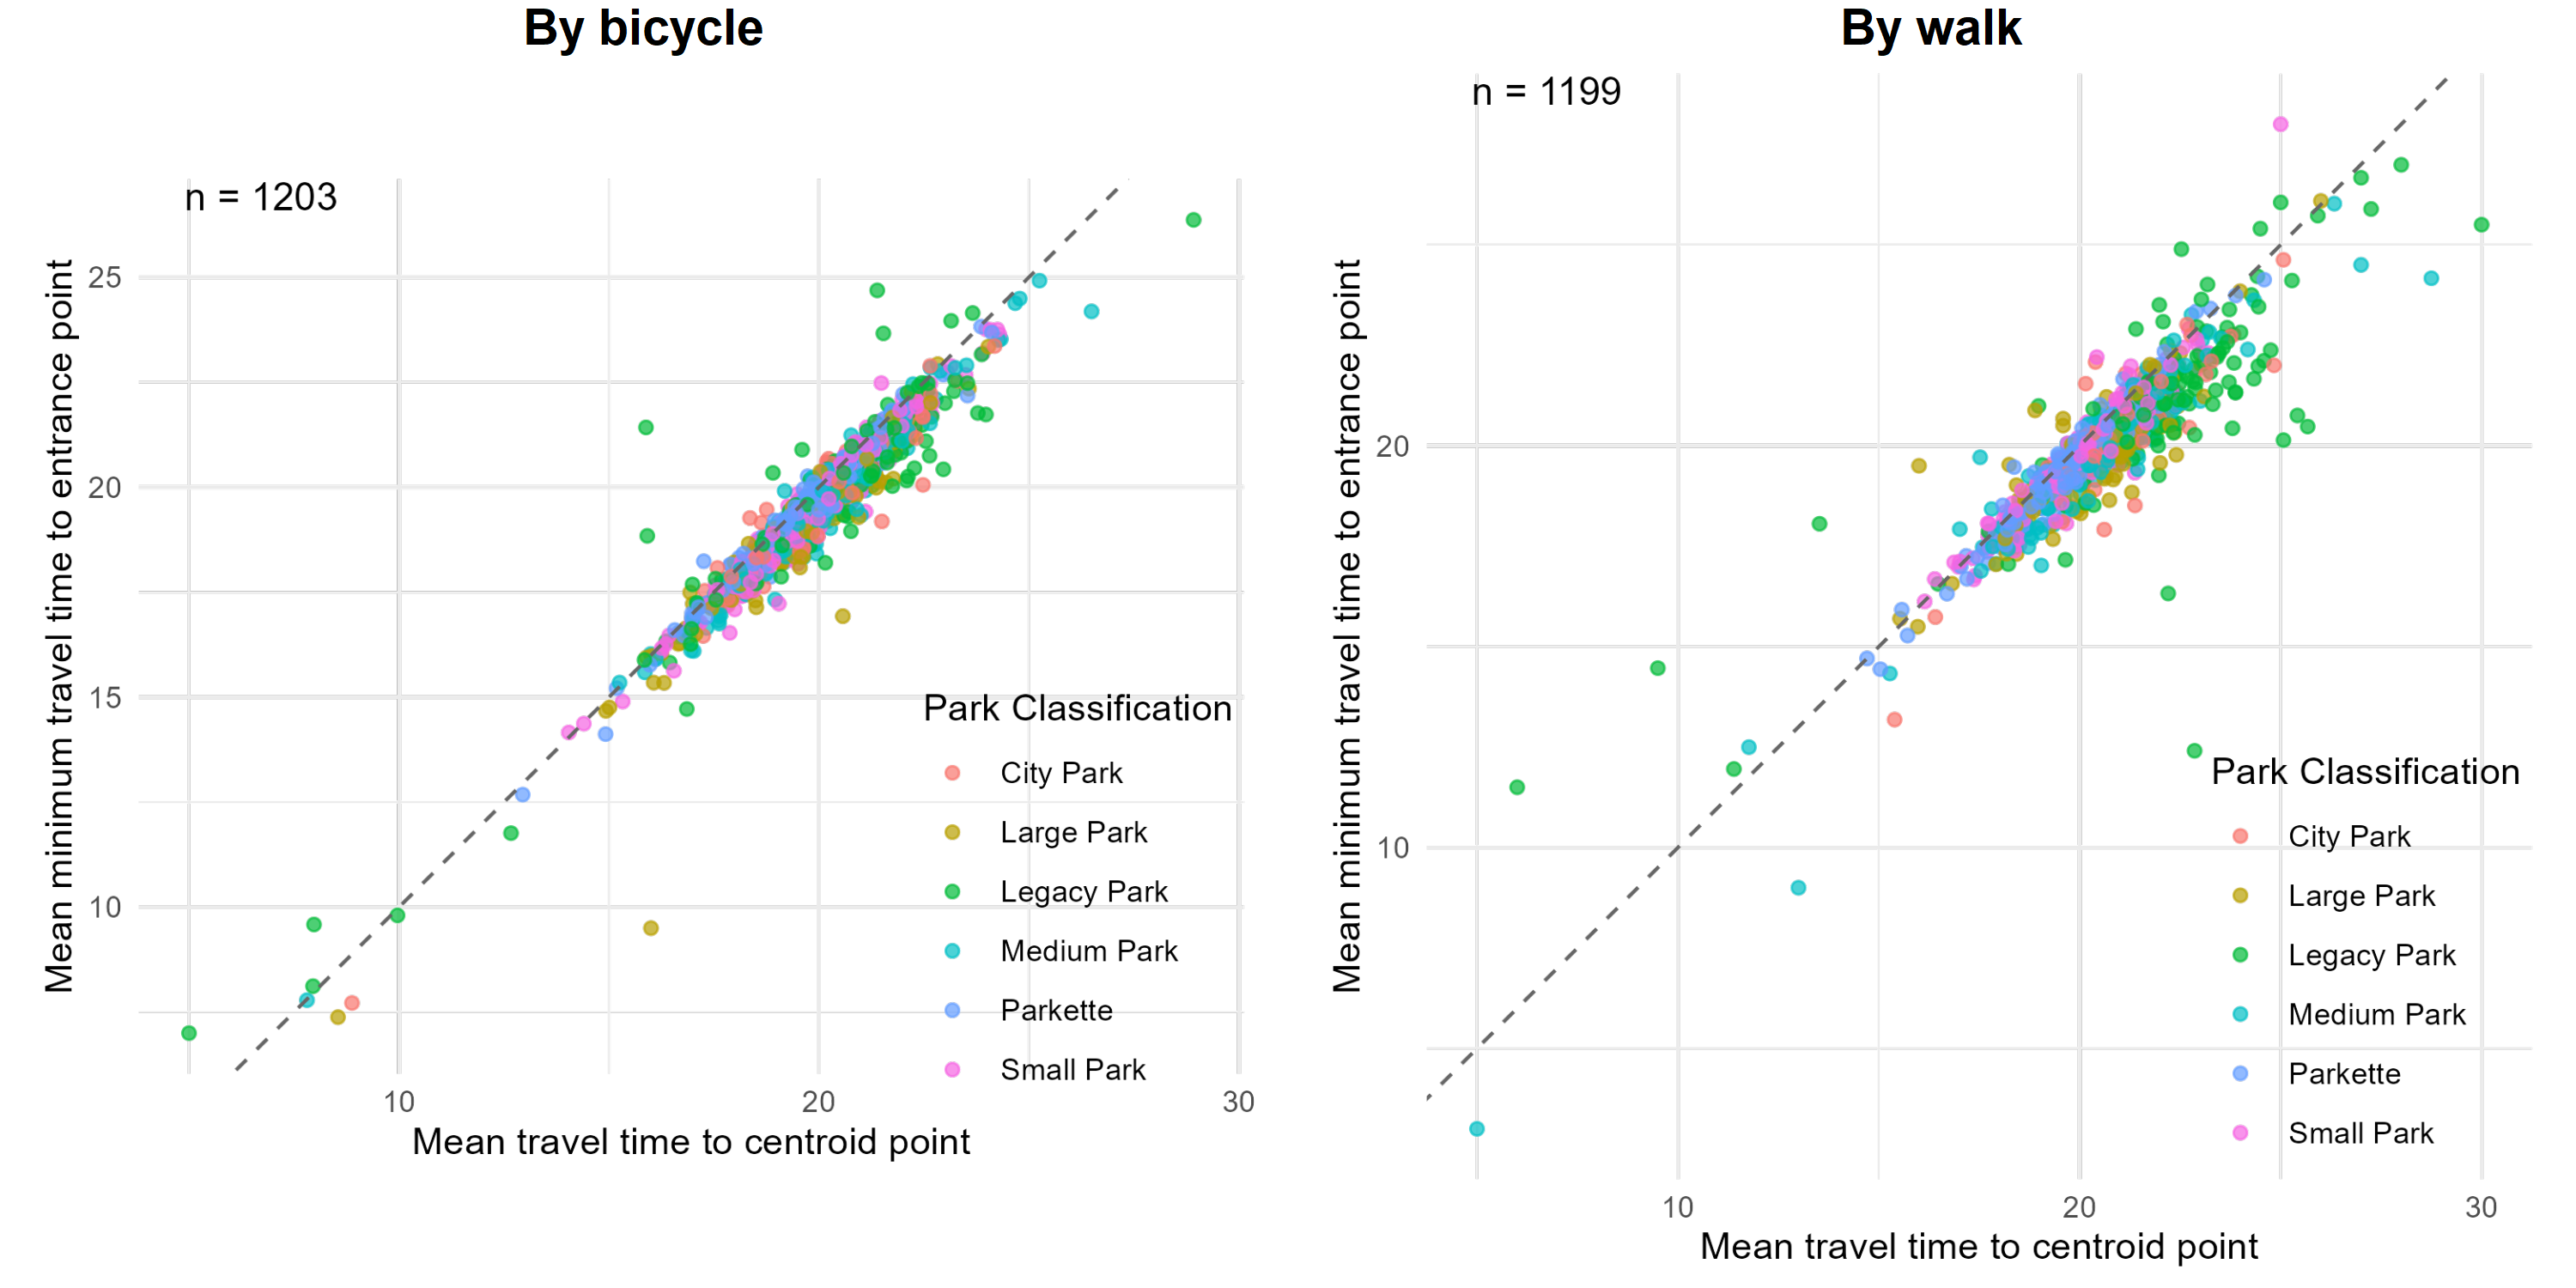
\includegraphics[width=6in]{./data/figures/chp3-ent_vs_cent_tt_walk_cycle_scatter} 

}

\caption{\label{fig:chp3-ent_vs_cent_tt_cycle_walk_scatter}  Scatter plot of cycle and walk travel times from origins to destinations by destination type for each park (either min mean travel time to park centroid, or to min mean travel time to park entrance). }\label{fig:unnamed-chunk-49}
\end{figure}

\subsubsection{Normative and empirical lengths of park-bound trips}\label{normative-and-empirical-lengths-of-park-bound-trips}

A key component of accessibility is how the cost of overcoming spatial separation to reach a destination is considered. As normative goals for planning modal parkland provision have not be explicitly specified by the City of Toronto, example normative trip lengths are defined. This definition is based on adhoc discussions with city staff and using distance catchments based on park size classifications from the City of Toronto (2019) report.

It is assumed that the smaller parks, i.e., parkette (\textless0.5ha), small parks (0.5-1.0 ha), and medium parks (1.5-3 ha) offer a service coverage of only 0.5km, 1.0km and 1.5km, respectively. Meaning, people are only likely to interact with the park within this travel distance. This assumption has to do with the qualities these parks possess, and the availability of similar parks in the area: namely, these smaller parks are often located in residential neighbourhoods, evenly spatially distributed, and often offer no exceptional amenity that cannot be substituted by another similarly sized park nearby as inferred from City of Toronto (2019). For larger parks, such as large parks (3-5 ha), city parks (5-8 ha), and legacy parks (8+ ha), their service catchments are larger as they are more unique, attractive, and harder to substitute parks, as inferred from the City of Toronto (2019) report. Large parks are assumed a service coverage of 3km and city and legacy parks are assumed to be attractive, and hence cover, the whole city.

Hence, normative trip lengths in this dissertation are assumed to vary by park classification (as defined in City of Toronto (2019)), travel mode, and for the sake of communicability. It should be noted that this strategy is not the only possible approach; the City is due to develop a revised parkland strategy that may adopt different and more nuanced normative assumptions.

In other words, the following normative travel impedance functions are set based on trip lengths that are \emph{seen} as acceptable and easy to communicate. It is assumed that (1) non-motorized travelers are assumed not to travel over 15 minutes to any park, this includes all walking and cycling. For reference, 0.5 km travel distance (i.e., the `catchment' of parkettes) approximately translates to 8 mins of walking or 3 mins of cycling based on median routed travel speed. (2) transit users can access all types of parks, but based on a negative exponential distance decay function (\(f(c_{ij}) = e^{-0.02c_{ij}}\)). This function was selected as it yields a median travel time of approximately 30 minutes, meaning that half of the total weight of the travel impedance function--representing the spatial separation between people and parks--comes from trips between 0 to 30 minutes, and the other half comes from trips between 30 to 120 minutes. The function captures the idea that the deterrent effect of distance increases gradually, assigning progressively less `spatial interaction' weight to more distant parks, even though they remain reachable. (3) Car users are assumed \emph{not} to travel to smaller parks (i.e., Parkette, small and medium parks) at all, and as such, these parks are excluded from accessibility results for the car mode. For larger parks (i.e., large, city and legacy parks), car travel impedance is assumed also based on a negative exponential distance decay function, but with parameter \(-0.04\) (\(f(c_{ij}) = e^{-0.04c_{ij}}\)), twice as steep as the transit impedance function. This reflects a stronger deterrent effect with increasing travel time. Namely, with a median travel time of approximately 17 minutes, trips that are between 0 to 17 minutes are assigned half the weight of the travel impedance function and the remaining half is diffused across trips that are between 17 minutes to 120 minutes. Destinations 120 minutes are considered effectively unreachable, with the function modeled as 0 beyond this point for both transit and car modes.

These assumptions on interaction with parks and trip lengths by mode have equity implications:

\begin{itemize}
\tightlist
\item
  Smaller parks are assumed to only be attractive to, hence accessible for, non-motorized and transit users.
\item
  For larger parks which can be reached by all modes, car mode has the largest range and has a steep decay, meaning it may provide favourable spatial separation weight, relative to other modes.
\item
  Travel impedance for transit users is penalized more gradually, assuming broader reach to all park types.
\item
  Non-motorized users reach is constrained practically: they are assumed not to travel beyond 15 minutes.
\item
  For parks in less densely populated areas, i.e., with travel times by sustainable modes beyond 15 minutes, accessibility will only be present for car users. In sum, individuals in these areas who do not have access to a vehicle are effectively excluded.
\end{itemize}

To summarise the modal \(m\) travel behaviour based on parkland classification type \(y\) as the resulting travel impedance functions \(f^m(c^m_{ij})\) in Table \ref{tab:chp3-travel-impedance-by-park-mode}:

\begin{table}[ht]
\centering
\small
\begin{tabular}{|l|c|c|c|c|}
\hline
\textbf{Park Type} & \textbf{Car} & \textbf{Transit} & \textbf{Cycling} & \textbf{Walking} \\
\hline
Parkette &
0 $\forall$ $c_{ij}$ &
$e^{-0.02} \cdot c_{ij}^{\text{transit}}$ &
$1$ if $c \leq 15$ min, else 0 &
$1$ if $c \leq 15$ min, else 0 \\
\hline
Small Park &
0 $\forall$ $c_{ij}$ &
$e^{-0.02} \cdot c_{ij}^{\text{transit}}$ &
$1$ if $c_{ij} \leq 15$ min, else 0 &
$1$ if $c_{ij} \leq 15$ min, else 0 \\
\hline
Medium Park &
0 $\forall$ $c_{ij}$ &
$e^{-0.02} \cdot c_{ij}^{\text{transit}}$ &
$1$ if $c \leq 15$ min, else 0 &
$1$ if $c \leq 15$ min, else 0 \\
\hline
Large Park &
$e^{-0.04} \cdot c_{ij}^{\text{car}}$ &
$e^{-0.02} \cdot c_{ij}^{\text{transit}}$ &
$1$ if $c \leq 15$ min, else 0 &
$1$ if $c \leq 15$ min, else 0 \\
\hline
City Park &
$e^{-0.04} \cdot c_{ij}^{\text{car}}$ &
$e^{-0.02} \cdot c_{ij}^{\text{transit}}$ &
$1$ if $c \leq 15$ min, else 0 &
$1$ if $c \leq 15$ min, else 0 \\
\hline
Legacy Park &
$e^{-0.04} \cdot c_{ij}^{\text{car}}$ &
$e^{-0.02} \cdot c_{ij}^{\text{transit}}$ &
$1$ if $c \leq 15$ min, else 0 &
$1$ if $c \leq 15$ min, else 0 \\
\hline
\end{tabular}
\caption{Normative travel impedance functions by parkland classification $y$ and mode $m$}
\label{tab:chp3-travel-impedance-by-park-mode}
\end{table}

To reiterate, the trip length based travel time behaviour summarised in Table \ref{tab:chp3-travel-impedance-by-park-mode} are \emph{normative}--they represent a statement about what should be considered a reasonable travel time that defines parkland accessibility (A. Paez et al., 2012). In practice, however, travel behaviour empirically may diverge from these normative statements. For example, empirical data from the 2022 Transportation Tomorrow Survey of trips made for `leisure' purposes by different modes in the Greater Toronto Area region, reveals different patterns (Data Management Group, 2023). Figure \ref{fig:chp3-norm_pos_impedance_mode_parktype_plot} compares this normative travel behaviour (green lines) from Table \ref{tab:chp3-travel-impedance-by-park-mode} with the TTS empirically derived curves (dashed lines). For this analysis, the normative curves (i.e., Table \ref{tab:chp3-travel-impedance-by-park-mode}) are used to define accessibility. This will enable the interpretation of results in terms of what \emph{should} be accessible via each mode, according to planning goals, rather than what currently is based on observed travel behaviour.

\begin{figure}

{\centering 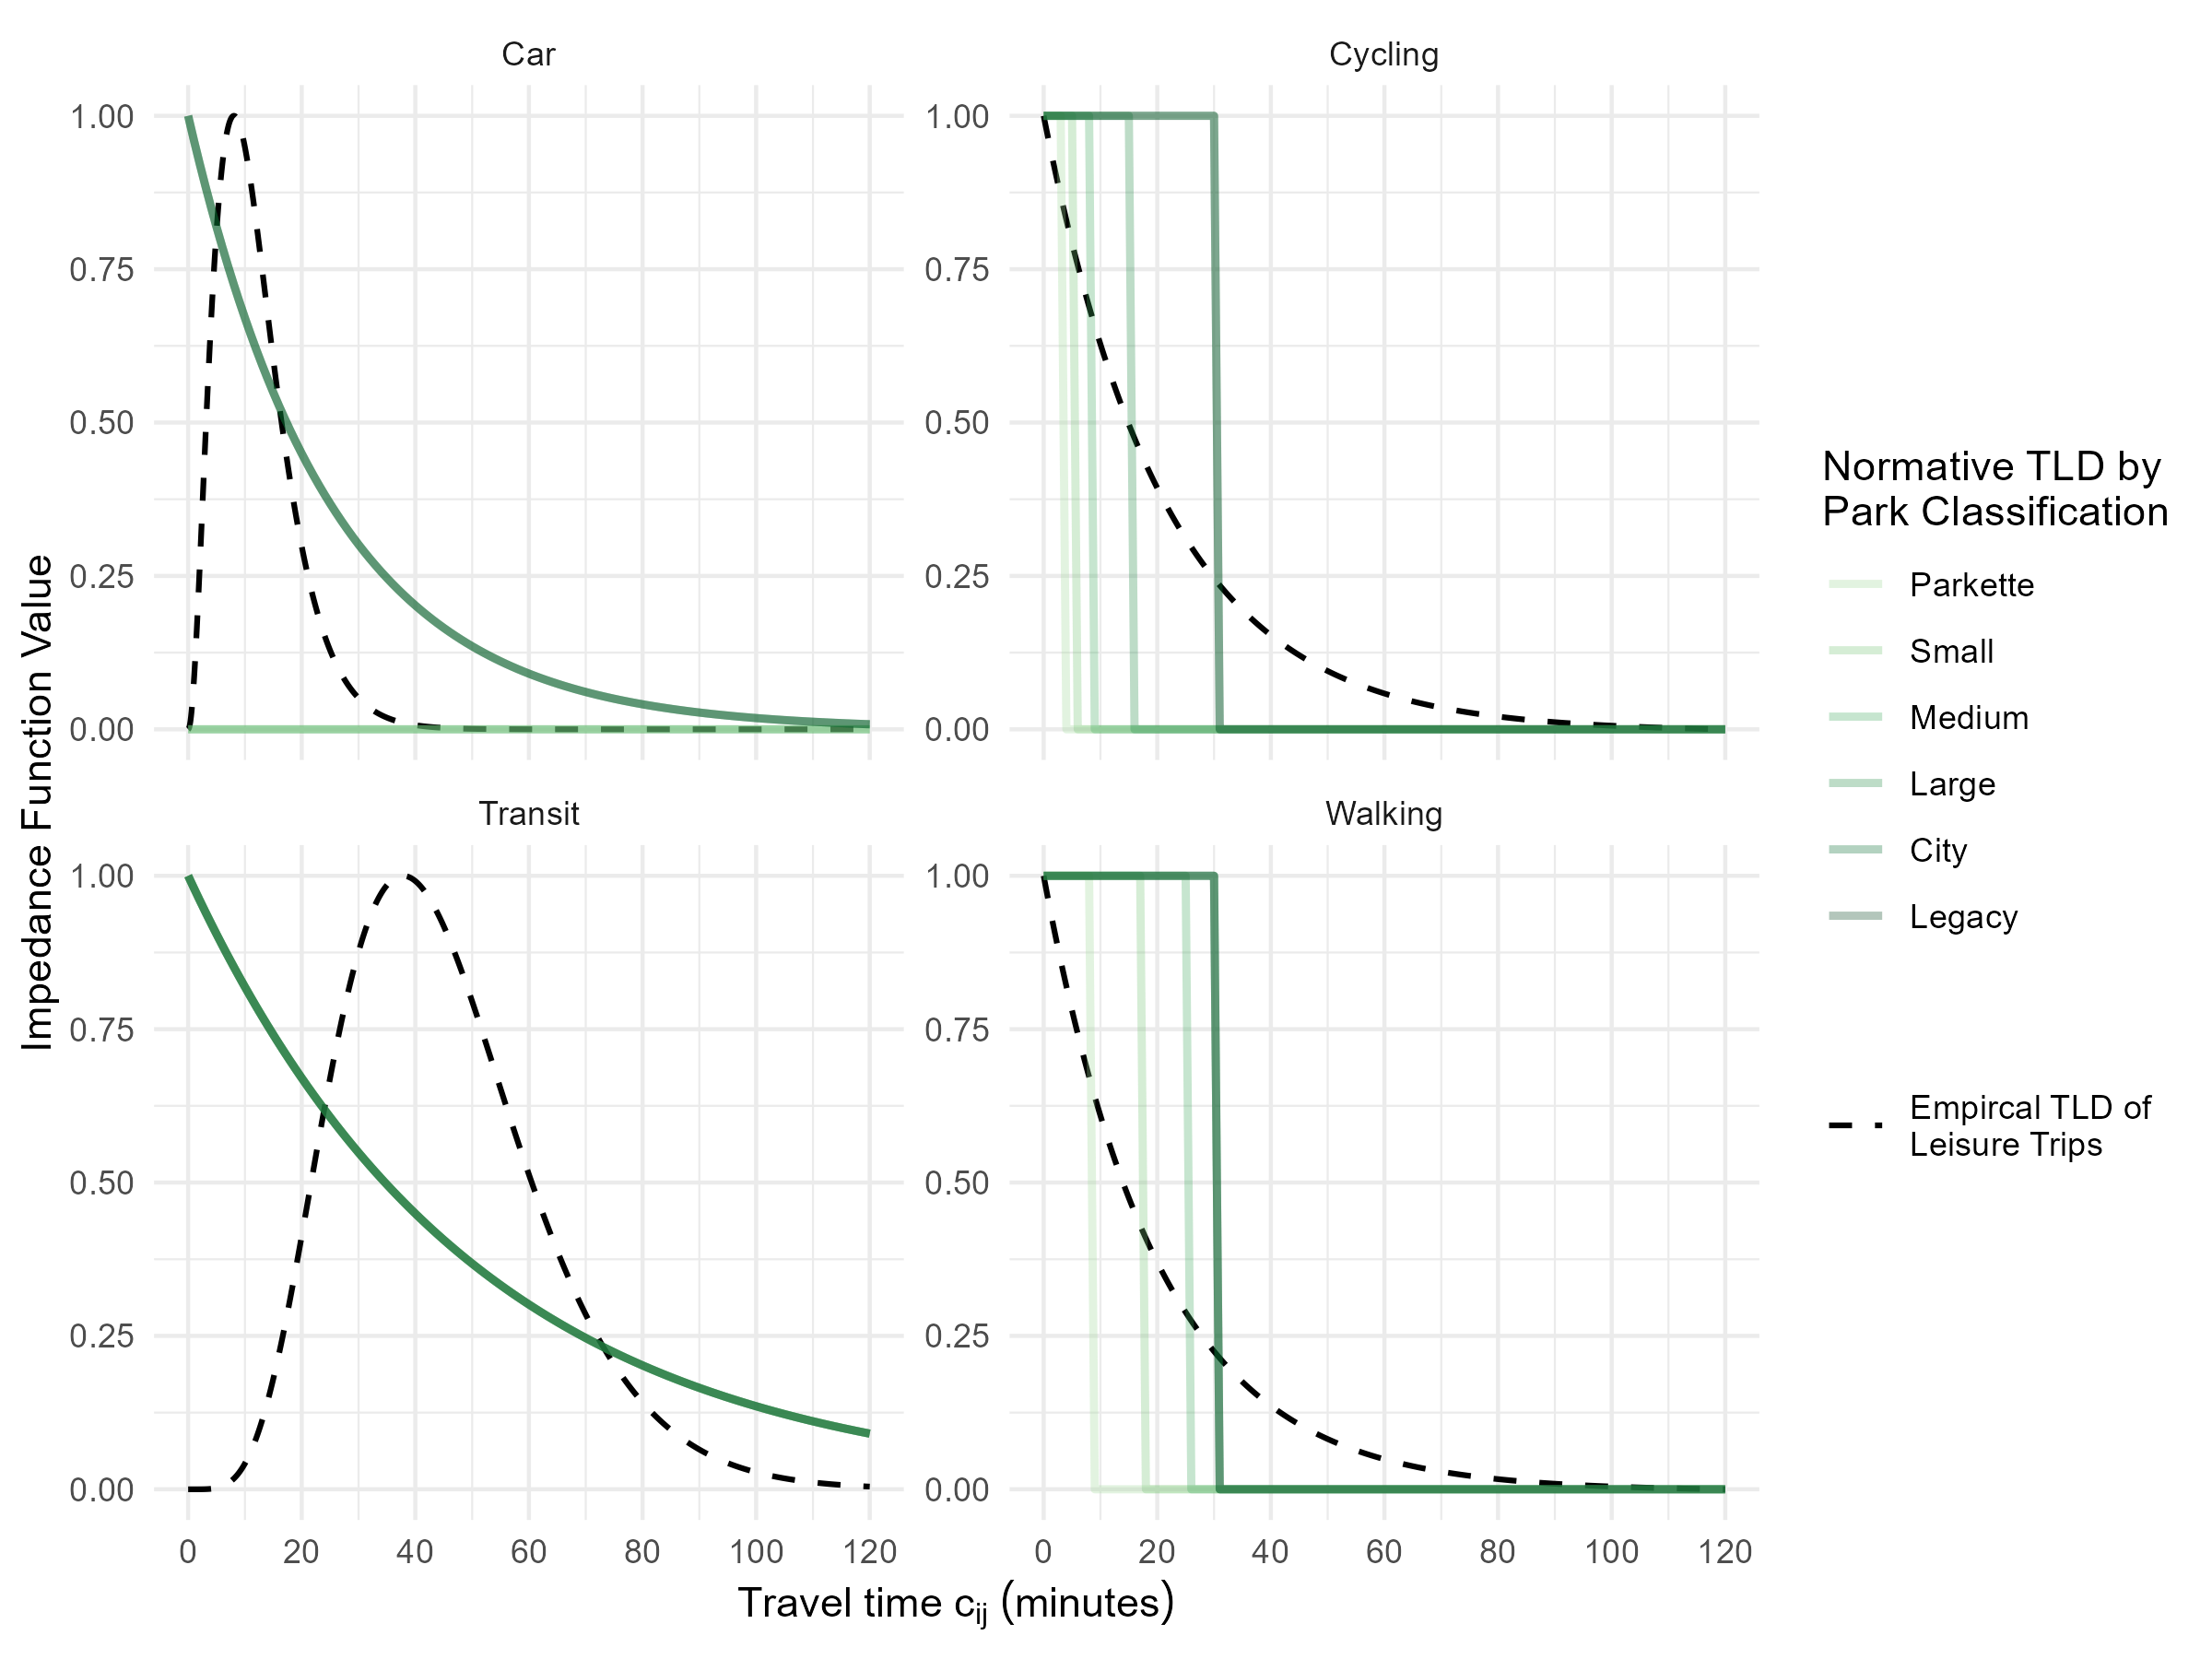
\includegraphics[width=6in]{./data/figures/chp3-norm_pos_impedance_mode_parktype_plot} 

}

\caption{\label{fig:chp3-norm_pos_impedance_mode_parktype_plot}  Scatter plot of cycle and walk travel times from origins to destinations by destination type for each park (either min mean travel time to park centroid, or to min mean travel time to park entrance). }\label{fig:unnamed-chunk-50}
\end{figure}

\subsubsection{Origin-side and destination-side mode-share}\label{origin-side-and-destination-side-mode-share}

In the multimodal extension of the singly constrained measure, the proportion of trips from each DB is assumed to follow a given modal split. This is based on the 2022 Transportation Tomorrow Survey (TTS), which includes a sample of 232,555 leisure trips made in the city of Toronto. Trips are grouped by mode as either transit, walking, cycling, or car. The survey data is structured as origin-destination flows and uses the Traffic Analysis Zones (TAZ) system, consisting of 940 zones across the City of Toronto--fewer than the 13,322 DBs used as origins and the 1,607 parks used as destinations--but still representative of the observed travel behaviour in the city to all `leisure' destinations (which include visits to parks, among other leisure activities). Unfortunately, disaggregating further by trip purpose was not available from the TTS.

For the \emph{accessible parkland} measures (i.e., the variant reflecting accessible parkland from an origin zone), origin-side modal splits from the TTS is retained. Each DB, the most granular origin zone used in this analysis, is spatially linked to the TTS zoning system and inherits the modal split of the TAZ it intersects. However, not all DBs fall within TAZs containing leisure trip data: some TAZs have no trips of this type that occur. In such cases (specifically for 131 of the 13,322 DBs), the average modal proportions from the parent Dissemination Area (DA) were used. If no leisure trips were observed at the DA level, the average for the corresponding Census Tract was used.

Through this approach, all DBs are assigned modal proportions that reflect the observed mode split for leisure trips in the TTS. These assigned proportions are shown in Figure \ref{fig:chp3-mode_split_eachDB_plots}. Notably, areas with high walking shares align closely with the downtown core and other built-up areas of the city, while these same areas display lower car mode shares.

\begin{figure}

{\centering \includegraphics[width=6in]{./data/figures/chp3-mode_split_eachDB_plots} 

}

\caption{\label{fig:chp3-mode_split_eachDB_plots}  The proportion of leisure trips by mode on a scale from 0 to 1. Trips are gleaned from the 2022 TTS. }\label{fig:unnamed-chunk-51}
\end{figure}

For the \emph{accessible population} variant of the singly constrained measure, mode share at the destination is required. This is interpreted as the proportion of parkland that is accessible by each mode of transportation. Since detailed information about mode-specific park capacities (e.g., availability of parking for cars or bikes) is unavailable, the mode share of trips arriving at destination zones, again drawn from the 2022 TTS leisure trip subset, is used as a proxy.

The method for assigning these mode shares to parks follows a similar approach to that used for the described DBs. First, parks were spatially intersected with TAZs (as destinations), and the modal split of trips arriving in those TAZs was calculated and assigned to the corresponding parks. For parks located in TAZs with no recorded leisure trips, mode share values were backfilled using average proportions from the larger Planning Districts (16 in Toronto) associated with the TAZ zoning system. This was necessary for 67 parks.

Figure \ref{fig:chp3-mode_split_parks_plots} displays the average mode share of trips arriving at parks, grouped by park size. Similar to Figure \ref{fig:chp3-mode_split_eachDB_plots}, Figure \ref{fig:chp3-mode_split_parks_plots} demonstrates that car is the dominant mode. Walking is the second most common mode, although its share decreases as park size increases---while car usage increases. Transit ranks third, and cycling consistently has the lowest share.

\begin{figure}

{\centering 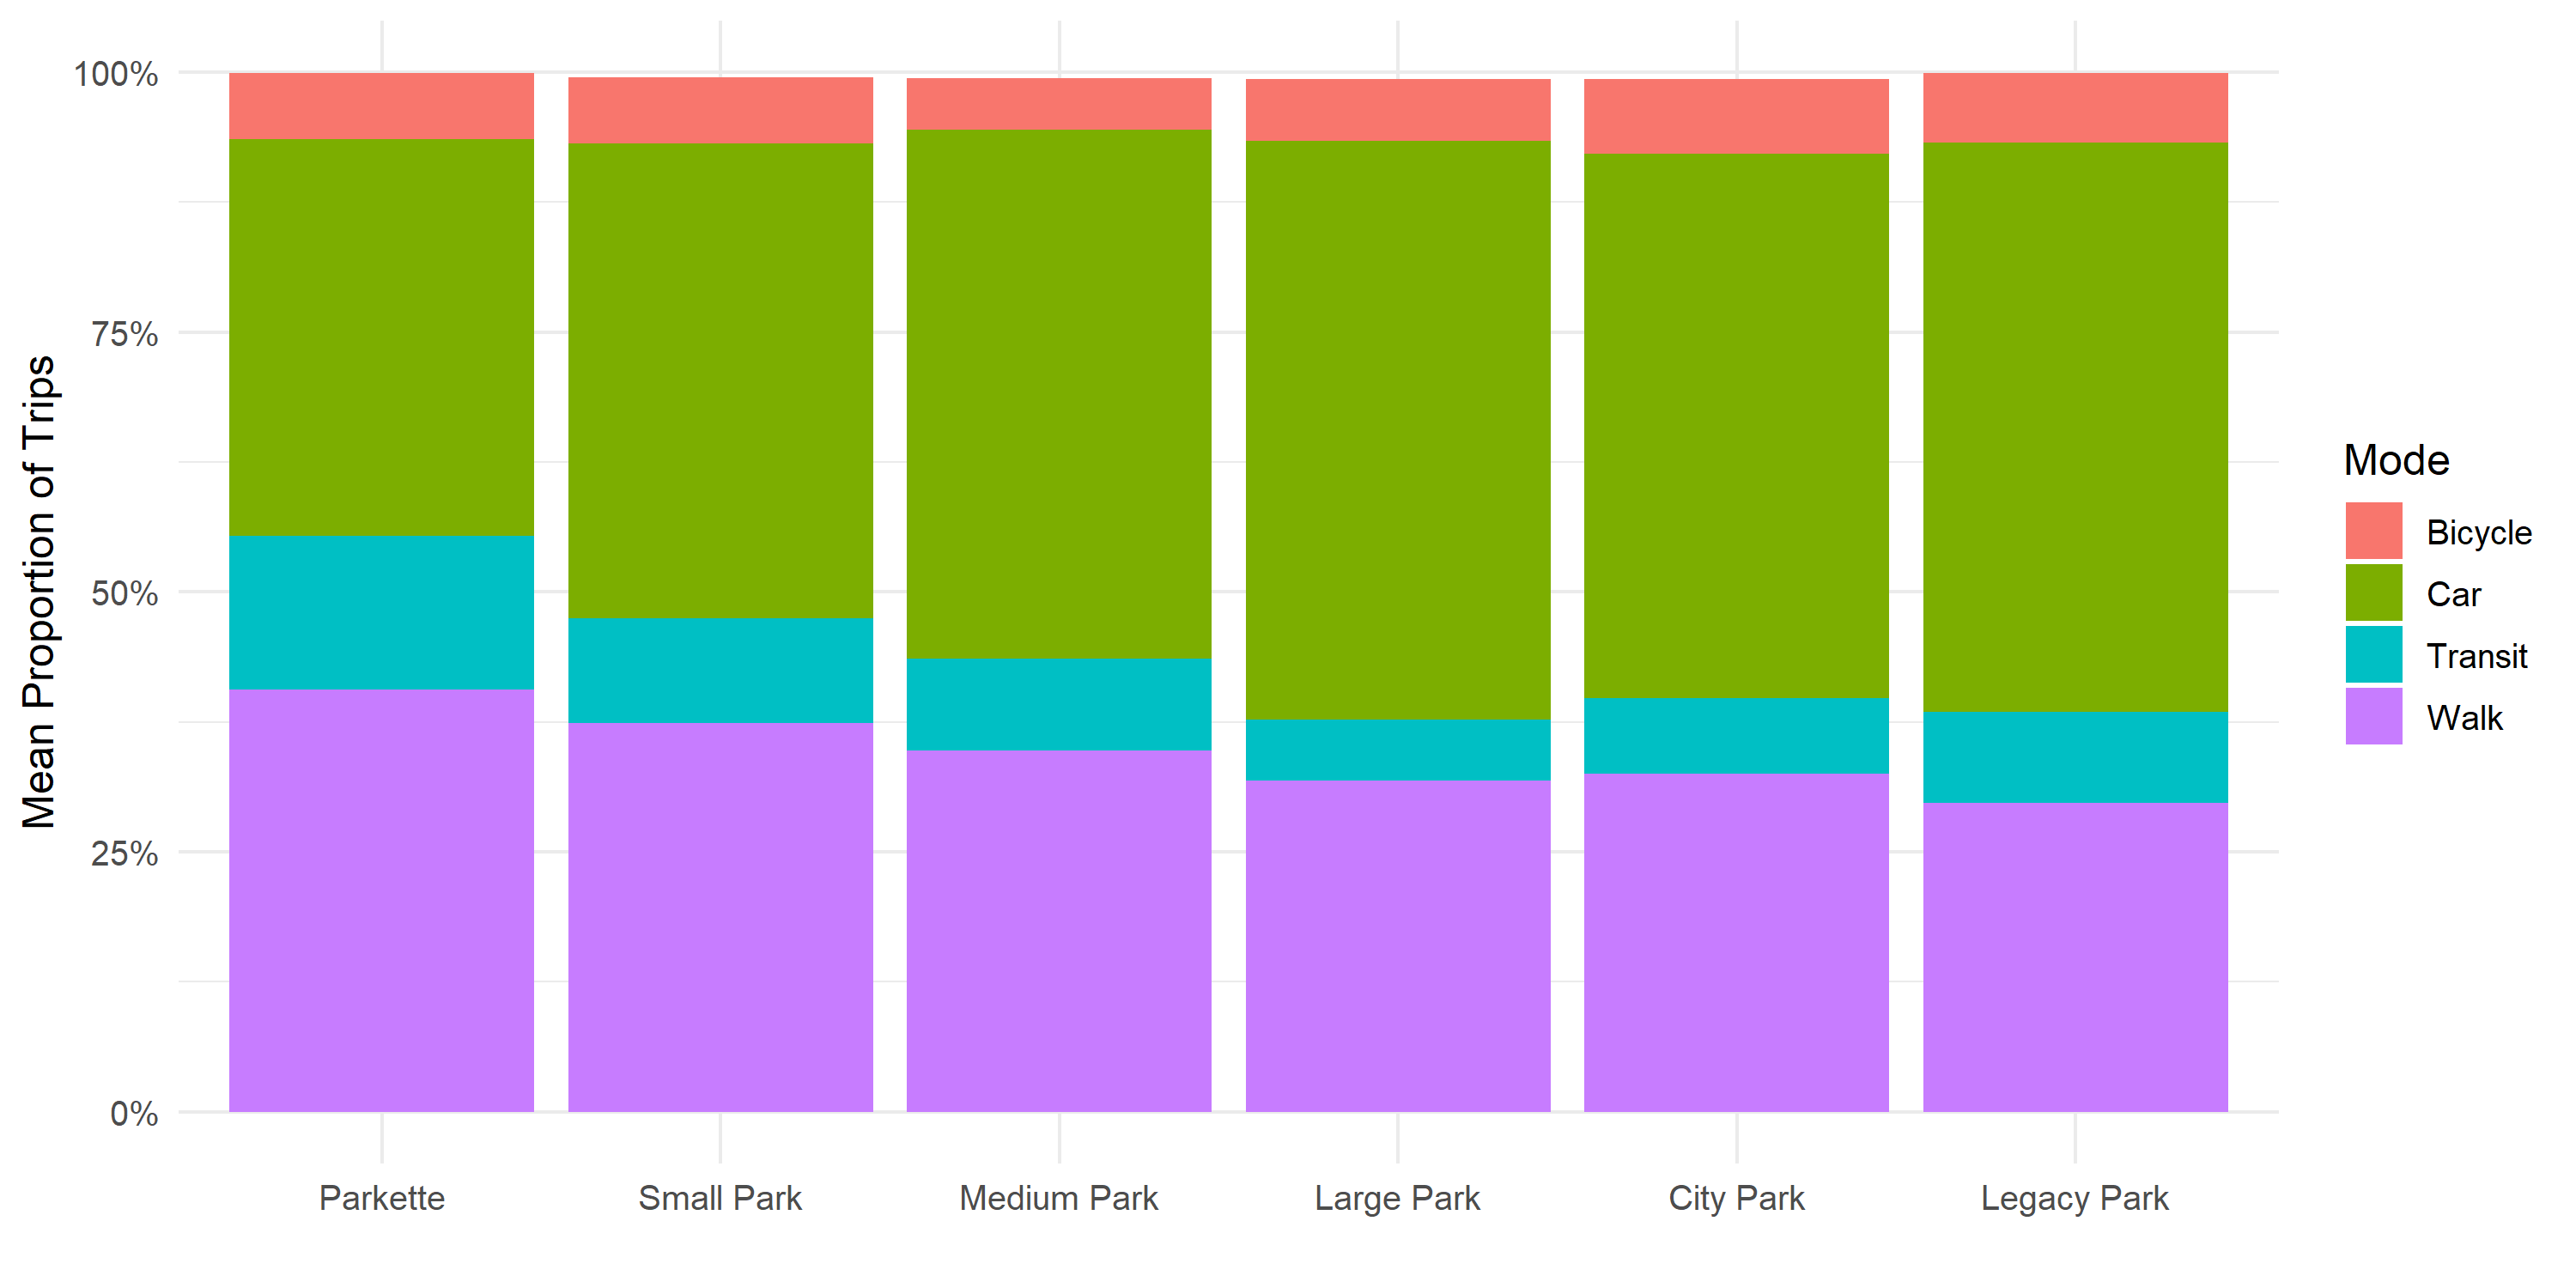
\includegraphics[width=6in]{./data/figures/chp3-mode_split_parks_plots} 

}

\caption{\label{fig:chp3-mode_split_parks_plots} The average proportion of leisure trips by mode arriving to a destination zone, as summarised by parks and park size. Trips are gleaned from the 2022 TTS. }\label{fig:unnamed-chunk-52}
\end{figure}

\section{Methods: constrainted and unconstrained accessibility measures}\label{methods-constrainted-and-unconstrained-accessibility-measures}

In this section, the methods outlined in Chapter 2 are specified for this empirical case study. Namely, the destination mass is defined as parkland area (opportunities) at the destination zone \(D_j\), the origin mass is defined as the number of people (population) at the origin zone \(O_i\), and their mode-specific origin-side and destination-side shares are defined in the their multimodal extension.

For \textbf{Chapter 4}, this includes:

\begin{enumerate}
\def\labelenumi{\arabic{enumi}.}
\tightlist
\item
  Unimodal total constrained \textbf{accessible parkland} summarised per each DB \(V_i^T\); All people to all parkland by walking is assessed: all people are assumed to walking. Each zonal value can be interpreted as ``how much parkland area is potentially reachable by the walking-population?''. It is also presented as a `parkland supply provision' ratio of parkland per population.
\item
  Unimodal total constrained \textbf{accessible population} summarised per park \(M_j^T\); the transpose of \(V_i^T\). Namely, all parkland to all people by walking will be assessed. Can be interpreted as ``how much walking-population is potentially reachable?'' from each park. Is presented as a potential population `service catchment' or a ratio of population potential per parkland area.
\item
  The first two measures are compared to a unimodal unconstrained \textbf{accessible parkland} summarised per each DB \(V_i^0\) and \textbf{accessible population} summarised per park \(M_j^0\), representing the traditional accessibility measure calculation method. Like the other two, all people (assumed to be walking) to all parkland are assessed, however the interpretation is different: instead the value is proportion to the ``the proportion of parkland area that is potentially reachable by the population from this park'' and proportional to ``the proportion of walking population that is potentially reachable by the park''. No `parkland provision' or `service catchment' ratios can be meaningfully calculated using these traditional methods.
\end{enumerate}

For \textbf{Chapter 5}, additional information concerning the modes \(m\) is introduced, namely: 1) the population at each origin DB is split to represent `walking', `cycling', `transit' and `car' modes based on observed TTS data, with their associated travel cost \(c_{ij}^m\) to parkland and travel impedance function \(f^m (c^m_{ij})\). And 2) the parkland at each destination is split to reflect the likelihood that they'll be visited by mode. This split is based on the parkland normative classification, namely that small parks are attractive based on walking and cycling impedance, while larger parks are attractive based on all modal impedance. The following measures are solved:

\begin{enumerate}
\def\labelenumi{\arabic{enumi}.}
\tightlist
\item
  Multimodal singly constrained \textbf{accessible parkland} summarised per mode and each DB \(V_i^{mS}\). All values can be interpreted as the proportion of parkland that is accessible as a function of the multimodal population and multimodal travel impedance for the specific-mode using group at \(i\).
\item
  Multimodal singly constrained \textbf{accessible population} summarised per mode and park destination \(M_j^{mS}\); Can be interpreted as the proportion of population that is accessible as a function of the multimodal parkland (i.e., magnetic quality associated with the park) and associated parkland travel impedance for the specific-mode using group at \(j\). This value is also presented as a potential population `service catchment' or a ratio of population potential per \(m\)-type of parkland area.
\item
  The first two measures are compared to unimodal unconstrained \textbf{accessible parkland} calculated for each mode summarised for each DB \(V_i^{0}\) and park \(M_j^{0}\), representing the traditional approach to calculating multimodal accessibility measure. \(V_i^{0}\) values are interpreted as parkland-area-modal-travel-impedance-value, or proportion to ``the proportion of parkland area that is potentially reachable by the mode-using-population from a zone''. No `parkland provision' ratio can be meaningfully calculated. Similar case for the interpretation of \(M_j^{0}\) and the inability to calculate a meaningful population `service catchment' ratio.
\end{enumerate}

And as a summary of the mathematical variables, across all equations in this empirical case study, the following definitions apply:

\begin{itemize}
\tightlist
\item
  Each zone can be either origins \(i\) or destinations \(j\) in the same system. However, in this empirical case \(i\)s and \(j\)s are distinct, but still within the same system (city of Toronto). Each \(i\) is a dissemination block (DB) and each destination is a park \(j\).
\item
  \(m\) is an index indicating the type of multimodal quality of either the origin-zone-mass (population) or destination-zone-mass (parkland); \(m\) is either ``walk'', ``cycle'', ``transit'' and ``car''.
\item
  \(f(c_{ij})\) is the function of the cost of travel expressed in travel time \(c_{ij}\) from \(i\) to \(j\). In the multimodal variation, \(f^m(c^m_{ij})\) is defined for different \(m\)s (e.g., travel time and the travel function from an origin to a destination for ``walk'' is distinct than ``car'')
\item
  the destination zone attraction mass \(W_j^{(2)}\) is the number of opportunities (i.e., the parkland in hectares at a park \(j\)); A multimodal expression of this mass is expressed as \(W_j^{m(2)}\). When \(W_j^{(2)}\) refers to a known marginal in a zone (i.e., parkland area at a \(j\) that is allocated or used for allocation) it is denoted as \(D_j\). When the \(\sum W_j^{(2)}\) is of interest, it refers to the known total destination-mass marginal sum in the region \(D\) (i.e., total parkland area in the city that is allocated).
\item
  the origin zone production mass \(W_i^{(1)}\) is the number of population (i.e., the population at a DB \(i\)); A multimodal expression of this mass is expressed as \(W_i^{m(1)}\). When \(W_i^{(1)}\) refers to a known marginal at the origin zone (i.e., population at a \(i\) that is allocated or used for allocation) it is denoted as \(O_i\). When \(\sum W_i^{(1)}\) is of interest, it is the known total marginal sum in the region \(O\) (i.e., total population in the city that is allocated).
\end{itemize}

\subsection{Methods for Chapter 4: unimodal accessibility}\label{methods-for-chapter-4-unimodal-accessibility}

\subsubsection{Unconstrained accessible parkland and population: proportional to the supply of parks and people reachable weighted by travel impedance}\label{unconstrained-accessible-parkland-and-population-proportional-to-the-supply-of-parks-and-people-reachable-weighted-by-travel-impedance}

A summary of \(V_{ij}^0\) for each \(i\) is:

\begin{equation}
\label{eq:unconstrained-accessibility-park}
V^0_i = \sum_j V^0_{ij} = \sum_j W^{(2)}_j f(c_{ij}) = S_i
\end{equation} 

Where \(V^0_{ij}\) is the number of parkland-area-\(f^\text{walk}(c^{walk}_{ij})\) at each \(i\) from \(j\). It can be summarised for each \(i\) and hence \(V^0_i\) is equivalent to Hansen's accessibility \(S_i\).

Likewise, the concept of market potential \(M_j^0\) expressed as a transpose of \(V^0_{ij}\):

\begin{equation}
\label{eq:unconstrained-market-park}
M_j^0 = \sum_i M^0_{ji} = \sum_i W_i^{(1)} f(c_{ij})
\end{equation} 

Where \(M^0_{ji}\) is the number of population-\(f^\text{walk}(c^{walk}_{ij})\) at each \(j\) from \(i\). It can be summarised for each \(j\) and hence expressed as \(M^0_j\).

\subsubsection{Total constrained accessibility:}\label{total-constrained-accessibility-1}

This member of the family of accessibility measures should be used when information that justifies constraining the opportunities (or population) at each zone is unavailable--leaving only the justification of allocating the regional total (of opportunities in the case of accessible opportunities or population in the case of accessible population).

In the variant of \textbf{accessible opportunities}, this situation arises when opportunities are not zonally competitive, that is, they can be freely allocated to zones based solely on travel impedance, without accounting for zonal demand of the population. In effect, this measure assumes the population demands the opportunities uniformly across each zone.

Similarly, for \textbf{accessible population}, this variant should be applied when population is treated as non-competitive. This measure freely allocates the total population to opportunity zones based on travel impedance, without considering the capacity or supply of those zones in terms of opportunity supply. This measure assumes the population is uniformly ``supplied'' to opportunities throughout the region.

\paragraph{Accessible parkland: constrained to the total supply of parkland.}\label{accessible-parkland-constrained-to-the-total-supply-of-parkland.}

~The total constrained accessible opportunities measure \(V^T_{i}\) now becomes Hansen's accessibility with a balancing factor \(K^T\):

\begin{equation}
\label{eq:total-constrained-accessibility-park}
V^T_i = \sum_j V^T_{ij} = K^T \sum_j W^{(2)}_j f(c_{ij}) = K^T V^0_i
\end{equation} 

Where:

\begin{itemize}
\tightlist
\item
  \(V^T_{ij}\) is the parkland area accessible at \(i\) from \(j\) that can be summarised as the parkland accessible at \(i\) \(V^T_{i}\);
\item
  \(K^T\) is the balancing factor reflecting the total constraint (Equation \ref{eq:total-constraint-accessibility}), i.e., ensuring that the sum of all the accessible parkland area is equal to the total parkland in the city (\(\sum_i\sum_j V^T_{ij} = \sum_i V^T_{i} = D\)) \(\frac{W^{(2)}_j}{\sum_i\sum_j W^{(2)}_jf(c_{ij})}\) that serves to proportionally allocate the opportunities \(D\) in the region and ensures units remain balanced.
\end{itemize}

Put another way: \(V^T_i\) sums all \(V^T_{ij}\) for a specific \(i\) (i.e., \(V^T_i = \sum_j V^T_{ij}\)). \(V^T_i\) is linearly proportional to the Hansen-type accessibility measure \(S_i = W^{(2)}_jf(c_{ij})\). Furthermore, \(V_{ij}^T\) can be written to be equal to \(\kappa_{ij}^T D\) where the dimensionless proportional allocation factor (\(\kappa_{ij}^T = \frac{W_j^{(2)} f(c_{ij})}{\sum_i\sum_j W^{(2)}_jf(c_{ij})}\)) allocates \(D\) to each \(i\) corresponding to each \(j\), explicitly communicating that each \(V_{ij}^T\) is a proportion of \(D\).

\paragraph{Accessible population: constrained to the total demanding population.}\label{accessible-population-constrained-to-the-total-demanding-population.}

~The total constrained accessible population measure now becomes traditional market potential with a balancing factor \(\hat K^T\):

\begin{equation}
\label{eq:total-constrained-market-park}
M^T_{j} = \sum_i M^T_{ji} = \hat K^T \sum_i W_i^{(1)} f(c_{ij}) = \hat K^T M_{j}^0
\end{equation} 

Where:

\begin{itemize}
\tightlist
\item
  \(M^T_{ji}\) is the number of population accessible at \(j\) from \(i\) that can be summarised as the population accessible at \(j\) \(M^T_{j}\),
\item
  \(\hat K^T\) is the balancing factor reflecting the total constraint, i.e., ensuring that the sum of all the accessible population is equal to the population in the city (\(\sum_i\sum_j M^T_{ji} = \sum_j M^T_{j} = O\)) \(\frac{W^{(1)}_i}{\sum_i\sum_j W^{(1)}_if(c_{ij})}\) that serves to proportionally allocate the population \(O\) in the region and ensures units remain balanced.
\end{itemize}

As well, \(M^T_{ji}\) can be written to be equal to \(\hat\kappa_{ij}^T O\) where the dimensionless proportional allocation factor (\(\hat \kappa_{ij}^T = \frac{W_i^{(1)} f(c_{ij})}{\sum_i\sum_j W^{(1)}_i f(c_{ij})}\)) allocates \(O\) to each \(j\) corresponding to each \(i\), explicitly communicating that each \(M^T_{ji}\) is a proportion of \(O\).

\subsubsection{Singly constrained accessibility:}\label{singly-constrained-accessibility-1}

This member of measure should be used when we know more information: namely, we know that the amount of parkland (or population) should be allocated based on the origin-mass demand (or destination-mass supply). This builds on the `total constrained' measure, where now the opportunities (or population) can be considered competitive (or responding to competition).

So: in the variant of \textbf{accessible opportunities}, this variant should be applied when opportunities are seen as zonally competitive, that is, they should be allocated to zones based on the population's zonal demand as well as travel impedance. This measure assumes the zonal demand of the population and distributes zonal opportunities based on this demand (and travel impedance).

Similarly, for \textbf{accessible population}, this variant should be applied when population is treated as zonally competitive, that is, population should be allocated to zones based on the zonal parkland supply as well as travel impedance. This variant assumes the zonal population is allocated to zones based on their opportunity ``supply'' (and travel impedance).

\paragraph{Accessible parkland: constrained to the total and marginal supply of parkland.}\label{accessible-parkland-constrained-to-the-total-and-marginal-supply-of-parkland.}

~The singly constrained accessible opportunities measure now becomes a competitive measure with a balancing factor \(B_j\):

\begin{equation}
\label{eq:opportunity-constrained-accessibility-park}
V^S_{i} = \sum_j V^S_{ij} = \sum_j B_j D_j W_i^{(1)} f(c_{ij})
\end{equation} 

Where:

\begin{itemize}
\tightlist
\item
  \(V^S_{ij}\) is the parkland area accessible considering population demand at \(i\) from \(j\). It can be summarised as \(V^S_{i}\): the parkland accessible at \(i\);
\item
  \(B_j\) is the balancing factor reflecting the opportunity constraint, i.e., ensuring that the sum of accessible parkland area considering population demand \(V^S_{ij}\) allocated from a specific \(j\) is equal to the parkland from that \(j\) (i.e., Equation \ref{eq:opportunity-constraint}: \(\sum_i V^S_{ij} =  D_j\)). This constraint also satisfies the total constraint (Equation \ref{eq:total-constraint-accessibility}) and ensures units remain balanced.
\end{itemize}

\(V_{ij}^S\) can be written to be equal to \(\kappa_{ij}^S D_j\) where the dimensionless proportional allocation factor (\(\kappa_{ij}^S = \frac{W_i^{(1)} f(c_{ij})}{\sum_i W_i^{(1)} f(c_{ij})}\)) allocates \(D_j\) to each \(i\), explicitly communicating that each \(i\) to \(j\) is a a proportion of \(D_j\) and implicitly \(D\).

\paragraph{Accessible population: constrained to the total and marginal demanding population.}\label{accessible-population-constrained-to-the-total-and-marginal-demanding-population.}

~The singly constrained accessible population measure now becomes traditional market potential with a balancing factor \(A_i\):

\begin{equation}
\label{eq:population-constrained-accessibility-park}
M^S_j = \sum_i M^T_{ji} = \sum_i A_i O_i W_j^{(2)} f(c_{ij})
\end{equation} 

Where:

\begin{itemize}
\tightlist
\item
  \(M^S_{ji}\) is the number of population accessible considering parkland supply at \(j\) from \(i\). It can be summarised as \(M^S_{j}\): the population accessible at \(j\);
\item
  \(A_i\) is the balancing factor reflecting the population constraint, i.e., ensuring that the sum of accessible population considering parkland supply \(V^M_{ij}\) allocated from a specific \(i\) is equal to the population from that \(i\) (i.e., Equation \ref{eq:population-constraint}: \(\sum_j M^S_{ji} =  O_i\)). This constraint also satisfies the total constraint (Equation \ref{eq:total-constraint-market}) and ensures units remain balanced.
\end{itemize}

\(M_{ji}^S\) can be written to be equal to \(\hat \kappa_{ij}^S O_i\) where the dimensionless proportional allocation factor (\(\hat \kappa_{ij}^S = \frac{W_j^{(2)} f(c_{ij})}{\sum_j W_j^{(2)} f(c_{ij})}\)) allocates \(D_i\) to each \(j\), explicitly communicating that each \(j\) to \(i\) is a proportion of \(O_i\) and implicitly \(O\).

\subsection{Methods for Chapter 5: Multimodal accessibility}\label{methods-for-chapter-5-multimodal-accessibility}

\subsubsection{Unconstrained accessible parkland and population by multiple modes}\label{unconstrained-accessible-parkland-and-population-by-multiple-modes}

A summary of \(V_{ij}^{m0}\) for each \(i\) is:

\begin{equation}
\label{eq:unconstrained-multimodal-accessibility-park}
V^{m0}_{i} = \sum_j V^{m0}_{ij} = \sum_j W_j^{(2)} f^m(c^m_{ij})
\end{equation} 

Where \(V^{m0}_{ij}\) is the amount of parkland-area-\(f^{m}(c^{m}_{ij})\) at each \(i\) from \(j\) for a specific \(m\). It can be summarised for each \(i\) and hence \(V^{m0}_i\) is equivalent to Hansen's accessibility \(S_i\) calculated for a specific mode \(m\).

Likewise, the concept of multimodal market potential expressed as a transpose of \(V^{m0}_{ij}\):

\begin{equation}
\label{eq:unconstrained-multimodal-market-park}
M_j^{m0} = \sum_i M^{m0}_{ji} = \sum_i W_i^{(1)} f^m(c^m_{ij})
\end{equation} 

Where \(M^{m0}_{ji}\) is the number of population-\(f^m(c^{m}_{ij})\) at each \(j\) from \(i\). It can be summarised for each \(j\) and hence expressed as \(M^{m0}_j\).

Both multimodal extensions \(V^{m0}_{i}\) and \(M^{m0}_{j}\) are not truly `multimodal', as they are not a function of \emph{all} modes in the system.

Instead, an analyst must adjust the units post-calculation (e.g., scaling, normalization) or select impedance functions to facilitate comparison across modes (potentially at the expense of accurately reflecting travel behavior). Such adjustments may introduce bias and/or adhoc methodologies. Hence, the raw unconstrained accessibility values themselves are challenging to compare due to their units. However, \(V^{m0}_{i}\) and \(M^{m0}_{j}\) are included as a point of comparison for the multimodal scenarios against the following accessibility measures (total constrained and singly constrained multimodal accessibility).

\subsubsection{Total constrained multimodal accessibility:}\label{total-constrained-multimodal-accessibility}

The multimodal extension of this member of measure should be used when more information is known about modes: similar to when one would use the unimodal version, but now this information must be known for multiple modes \(m\). In other words, the multimodal extension should be used when it is known that the amount of parkland (or population) should be allocated based on the origin-mass demand (or destination-mass supply) and the matching marginal is qualified by \(m\)-specific travel impedance function \(f^m(c^m_{ij})\) .

The multimodal extension of the \textbf{accessible opportunities} measure variant of this member should be applied when opportunities are seen as zonally competitive, that is, they should be allocated to zones based on a \(m\)-specific split of population's zonal demand as well as its corresponding \(m\) travel impedance. This measure could reflect the number of accessible parkland per \(m\) at an \(i\) based on the allocation of parkland from each \(j\) to the different \(m\)-populations at each \(i\) (and their associated \(m\) travel impedance). In this empirical example, there will be four values per \(i\), each reflecting the amount of parkland that is accessible for the `walking', `cycling', `transit-using' and `car-using' populations (different \(m\)s) given their different travel impedance (\(f^m(c^m_{ij})\)).

Similarly, the multimodal extension of the \textbf{accessible population} measure should be applied when population is treated as zonally competitive, that is, population should be allocated to zones based on the \(m\)-specific supply of parkland and their associated \(m\) travel impedance. In this empirical example, there will be four \(m\) specific values per park \(j\), each reflecting the amount of population that is accessible for the `walking', `cycling', `transit-using' and `car-using' populations (different \(m\)s) given their different travel impedance (\(f^m(c^m_{ij})\)).

\paragraph{Accessible parkland by modal-qualities of population: constrained to the total of parkland.}\label{accessible-parkland-by-modal-qualities-of-population-constrained-to-the-total-of-parkland.}

~The total constrained multimodal accessible opportunities measure \(V^{mT}_{i}\) now becomes a sort of multimodal composite Hansen's accessibility with mode-specific balancing factor \(K^{mT}\):

\begin{equation}
\label{eq:total-constrained-multimodal-access-park}
V^{mT}_{i} = \sum_j V^{mT}_{ij} = K^{mT} W_j^{(2)} f^m(c^m_{ij})
\end{equation} 

Where:

\begin{itemize}
\tightlist
\item
  \(V^{mT}_{ij}\) is the parkland area accessible at \(i\) from \(j\) for a specific \(m\) (either walking, cycling, transit or motorist)--a subset of the origin-mass (population) at that \(i\). It can be summarised as the parkland accessible at \(i\) for a specific \(m\) \(V^{mT}_{i}\);
\item
  \(K^{mT}\) is the balancing factor reflecting the total constraint (Equation \ref{eq:total-constraint-accessibility}), i.e., ensuring that the sum of all the accessible parkland area is equal to the total parkland in the city (\(\sum_m\sum_i\sum_j V^{mT}_{ij} = \sum_m \sum_i V^{mT}_{i} = D\)) \(\frac{W^{(2)}_j}{\sum_m\sum_i\sum_j W^{(2)}_jf^m(c^m_{ij})}\) that serves to proportionally allocate the opportunities \(D\) in the region and ensures units remain balanced.
\end{itemize}

\(V_{ij}^{mT}\) can be written to be equal to \(\kappa_{ij}^{mT} D\) where the dimensionless proportional allocation factor (\(\kappa_{ij}^{mT} = \frac{W_j^{(2)} f^m(c^m_{ij})}{\sum_m\sum_i\sum_j W^{(2)}_jf^m(c^m_{ij})}\)) allocates \(D\) to each \(m\) at \(i\) corresponding to opportunities at \(j\), explicitly communicating that each \(V_{ij}^{mT}\) is a proportion of \(D\).

\paragraph{Accessible population by modal-qualities of parks: constrained to the total demanding population.}\label{accessible-population-by-modal-qualities-of-parks-constrained-to-the-total-demanding-population.}

~The total constrained multimodal accessible population measure \(V^{mT}_{i}\) now becomes a sort of multimodal composite market potential with mode-specific balancing factor \(\hat K^{mT}\)::

\begin{equation}
\label{eq:total-constrained-multimodal-market-park}
M^{mT}_{j} = \sum_i M^{mT}_{ji} = \hat K^{mT} W_j^{(2)} f^m(c^m_{ij})
\end{equation} 

Where:

\begin{itemize}
\tightlist
\item
  \(M^{mT}_{ji}\) is the population accessible at \(j\) from \(i\) for a specific \(m\) (either walking, cycling, transit or motorist)--a subset of the destination-mass (population) at that \(i\). It can be summarised as \(M^{mT}_{j}\), the population accessible at \(j\) for a specific \(m\);
\item
  \(\hat K^{mT}\) is the balancing factor reflecting the total constraint (Equation \ref{eq:total-constraint-accessibility}) but from the perspective of the sum of the total population marginal, i.e., ensuring that the sum of all the accessible population is equal to the total population in the city (\(\sum_m \sum_i\sum_j M^{mT}_{ji} = \sum_m \sum_j M^{mT}_{j} = O\)) \(\frac{W^{(1)}_i}{\sum_m\sum_i\sum_j W^{(1)}_if^m(c^m_{ji})}\) that serves to proportionally allocate the opportunities \(D\) in the region and ensures units remain balanced.
\end{itemize}

\(M_{ji}^{mT}\) can be written to be equal to \(\hat \kappa_{ji}^{mT} O\) where the dimensionless proportional allocation factor (\(\hat \kappa_{ji}^{mT} = \frac{W_i^{(1)} f^m(c^m_{ji})}{\sum_m\sum_i\sum_j W^{(1)}_if^m(c^m_{ji})}\)) allocates \(O\) to each \(m\) at \(j\) corresponding to population at \(i\), explicitly communicating that each \(M_{ji}^{mT}\) is a proportion of \(O\).

\subsubsection{Singly constrained multimodal accessibility:}\label{singly-constrained-multimodal-accessibility}

This member of measure should be used when even more information about the modes are known: namely, we know not only know the amount of parkland (or population) that should be allocated based on the origin-mass demand (or destination-mass supply) but also specific types of \(m\) at each \(i\) (or \(j\)) and their associated \(f^m(c^m_{ij})\) that should dictate this proportional allocation. This extension on the `total constrained' multimodal measure, where now the opportunities (or population) can be considered competitive (or responding to competition) in a multimodal sense.

In the multimodal \textbf{accessible opportunities} variant, opportunities are seen as zonally competitive, that is, they should be allocated to origins based on the \(m\)-population's zonal demand as well as their \(m\) specific travel impedance. In this empirical example, there will four values per \(i\), each reflecting the amount of parkland that is accessible for the `walking', `cycling', `transit-using' and `car-using' populations (different \(m\)s) given their different travel impedance (\(f^m(c^m_{ij})\)) \emph{and} the proportion of their \(m\)-populations themselves.

Similarly, for the multimodal \textbf{accessible population} variant, population is treated as zonally competitive hence allocated to destinations based on the \(m\)-opportunity's zonal supply as well as their \(m\) specific travel impedance. In this empirical example, there will be four \(m\) specific values per park \(j\), each reflecting the amount of population that is accessible for the `walking', `cycling', `transit-using' and `car-using' populations (different \(m\)s) given their different travel impedance (\(f^m(c^m_{ij})\)) \emph{and} the proportion of their \(m\)-specific parkland themselves.

\paragraph{Accessible parkland by modal-qualities of population: constrained to the total and marginal supply of parkland.}\label{accessible-parkland-by-modal-qualities-of-population-constrained-to-the-total-and-marginal-supply-of-parkland.}

~The singly constrained multimodal accessible opportunities measure now becomes a competitive multimodal measure with a mode-specific balancing factor \(B_j^{m}\):

\begin{equation}
\label{eq:singly-constrained-multimodal-accessibility-park}
V^{mS}_{i} = \sum_j V^{mS}_{ij} = B_j^{m} D_j W_i^{m(1)} f^m(c^m_{ij})
\end{equation} 

Where:

\begin{itemize}
\tightlist
\item
  \(V^{mS}_{ij}\) is the parkland area accessible at \(i\) from \(j\) for a specific \(m\) (either walking, cycling, transit or motorist)--a subset of the origin-mass (population) considering \(m\)-population demand at \(i\)s and \(m\)-specific travel impedance.
\item
  \(B_j^{m}\) is the \(B_j\) considering \(m\)s and reflects the opportunity constraint, i.e., ensuring that the \(\sum_m V^{mS}_{ij}\) (sum of accessible parkland area considering population demand) allocated from a specific \(j\) is equal to the parkland from that \(j\) (i.e., Equation \ref{eq:opportunity-constraint}: \(\sum_m \sum_i V^{nS}_{ij} =  D_j\)). This constraint also satisfies the total constraint (Equation \ref{eq:total-constraint-accessibility}) and ensures units remain balanced.
\end{itemize}

\(V_{ij}^{mS}\) can be written to be equal to \(\kappa_{ij}^{mS} D_j\) where the dimensionless proportional allocation factor (\(\kappa_{ij}^{mS} = \frac{W_i^{m(1)} f^m(c^m_{ij})}{\sum_m\sum_i W_i^{m(1)} f^m(c^m_{ij})}\)) allocates \(D_j\) to each \(m\) at each \(i\), explicitly communicating that each \(m\) at each \(i\) to \(j\) is a proportion of \(D_j\) and implicitly all sums to equal \(D\).

\paragraph{Accessible population by modal-qualities of parks: constrained to the total and marginal demanding population.}\label{accessible-population-by-modal-qualities-of-parks-constrained-to-the-total-and-marginal-demanding-population.}

~The singly constrained multimodal accessible population measure now becomes a competitive multimodal measure with a mode-specific balancing factor \(A_i^{m}\)::

\begin{equation}
\label{eq:singly-constrained-multimodal-market-park}
M^{mS}_{ji} = \sum_i M^{mS}_{ji} = A_i^{m} O_i W_j^{m(2)} f^m(c^m_{ij})
\end{equation} 

Where:

\begin{itemize}
\tightlist
\item
  \(M^{mS}_{ji}\) is the population accessible at \(j\) from \(i\) for a specific \(m\) (either walking, cycling, transit or motorist)--a subset of the destination-mass (opportunity) considering \(m\)-parkland supply at \(j\)s and \(m\)-specific travel impedance.
\item
  \(A_i^{m}\) is the \(A_i\) considering \(m\)s and reflects the population constraint, i.e., ensuring that the \(\sum_m M^{mS}_{ji}\) (sum of accessible population considering parkland supply) allocated from a specific \(i\) is equal to the population from that \(i\) (i.e., Equation \ref{eq:population-constraint}: \(\sum_m \sum_j M^{mS}_{ji} = O_i\)). This constraint also satisfies the total constraint (Equation \ref{eq:total-constraint-accessibility}) and ensures units remain balanced.
\end{itemize}

\(M_{ji}^{mS}\) can be written to be equal to \(\hat \kappa_{ji}^{mS} O_i\) where the dimensionless proportional allocation factor (\(\hat \kappa_{ji}^{mS} =  \frac{W_j^{m(2)} f^m(c^m_{ij})}{\sum_m\sum_j W_j^{m(2)} f^m(c^m_{ij})}\)) allocates \(O_i\) to each \(m\) at each \(j\), explicitly communicating that each \(m\) at each \(j\) to \(i\) is a proportion of \(O_i\) and implicitly all sums to equal \(O\).

\subsection{For both Chapter 4 and 5: Representing constrained accessibility as a ratios}\label{for-both-chapter-4-and-5-representing-constrained-accessibility-as-a-ratios}

Referring to \textbf{accessible opportunities}, i.e., \(V_{ij}^T\) \& \(V_{ij}^{mT}\), and \(V_{ij}^{S}\) \& \(V_{ij}^{mS}\), are represented per capita and aggregated at different zonal levels to reflect \textbf{potential parkland provision}:

Accessible parkland area per capita at a DB from the perspective of total constrained accessibility:

\begin{equation}
\label{eq:total-constrained-access-per-capita}
v^{T}_{i} = \frac{V^{T}_{i}}{O_{i}}
\end{equation} 

Total constrained multimodal accessible parkland area per \(m\) per capita at a DB:

\begin{equation}
\label{eq:total-constrained-multimodal-access-per-capita}
v^{mT}_{i} = \frac{V^{mT}_{i}}{O^{m}_{i}}
\end{equation} 

Singly constrained accessible parkland area per capita at a DB:

\begin{equation}
\label{eq:singly-constrained-access-per-capita}
v^{S}_{i} = \frac{V^{S}_{i}}{O_{i}}
\end{equation} 

Singly constrained multimodal accessible parkland area per \(m\) per capita at a DB:

\begin{equation}
\label{eq:singly-constrained-multimodal-access-per-capita}
v^{mS}_{i} = \frac{V^{mS}_{i}}{O^{m}_{i}}
\end{equation} 

This can likewise be applied to market potential. Referring to \textbf{accessible population}, i.e., summaries of \(M_{ji}^T\) \& \(M_{ji}^{mT}\), and \(M_{ji}^{S}\) \& \(M_{ji}^{mS}\), are represented per parkland type and aggregated at different zonal levels to reflect \textbf{potential population serviced}.

Total constrained accessible population per parkland area at a park:

\begin{equation}
\label{eq:total-constrained-market-per-capita}
m^{T}_{j} = \frac{M^{T}_{j}}{D_{j}}
\end{equation} 

Total constrained multimodal accessible population per \(m\) per parkland area at a park:

\begin{equation}
\label{eq:total-constrained-multimodal-market-per-capita}
m^{mT}_{j} = \frac{M^{mT}_{j}}{D^{m}_{j}}
\end{equation} 

Singly constrained accessible population per parkland area at a park:

\begin{equation}
\label{eq:singly-constrained-market-per-capita}
m^{S}_{j} = \frac{M^{S}_{j}}{D_{j}}
\end{equation} 

Singly constrained multimodal accessible population per \(m\) per parkland area at a park:

\begin{equation}
\label{eq:singly-constrained-multimodal-market-per-capita}
m^{mS}_{j} = \frac{M^{mS}_{j}}{D^{m}_{j}}
\end{equation} 

\section{Chapter conclusions}\label{chapter-conclusions-1}

This chapter includes all the City of Toronto population and parkland data included in the accessibility analysis (chapters 4 and 5) as well as the restatement of accessibility equations with respect to this case study.

\chapter{Unimodal accessibility to parks in Toronto}\label{unimodal-accessibility-to-parks-in-toronto}

\section{Overview}\label{overview-3}

In this chapter, walking accessibility (i.e., unimodal) of parkland and population is presented: where population is assumed to be all people at each DB and parkland is in hectares per park. We adopt the normative impedance function for walking discussed in Chapter 3, i.e., if a park entrance can be reached within 15 minutes of walking than the park is assumed to be reachable and enters the calculation as a 1, and if not, it is assumed full not reachable and enters the accessibility calculation as a 0.

In the first half of the chapter the focus is on \emph{accessible parkland area}. Values of \(V^0_i\), \(V^T_i\) and \(V^S_i\) are expressed at the DB level and at the neighbourhood level. Then, the accessible parkland per capita ratio is demonstrated, neighbourhoods are ranked and a discussion is detailed based on `potential parkland service provision'. In the second half of the section, \emph{accessible population} \(M^0_j\), \(M^T_j\) and \(M^S_j\) is presented per park and per parkland area ratios at the level of the park itself and the neighbourhood is discussed as the `potential population served'.

\section{Accessible parkland (for the population)}\label{accessible-parkland-for-the-population}

Figure \ref{fig:chp4-parkland_access_DB_WALK_plots} demonstrates that the unconstrained, total constrained (i.e., without population competition) and singly constrained accessible parkland (i.e., with population competition). All three plots are binned by quartile: 0-25th, 25-50th, 50-7th, 75th-100th. Light grey areas are DBs with 0 parkland accessibility. Grey DBs have population but have no parkland accessibility, as their representative DB point cannot reach an assumed parkland entrance within 15 minutes of walking. These grey DBs are often in proximity to light grey DBs and typically are larger in area, contain limited pedestrian infrastructure, and fewer connections into parks that are proximate.

\begin{figure}

{\centering 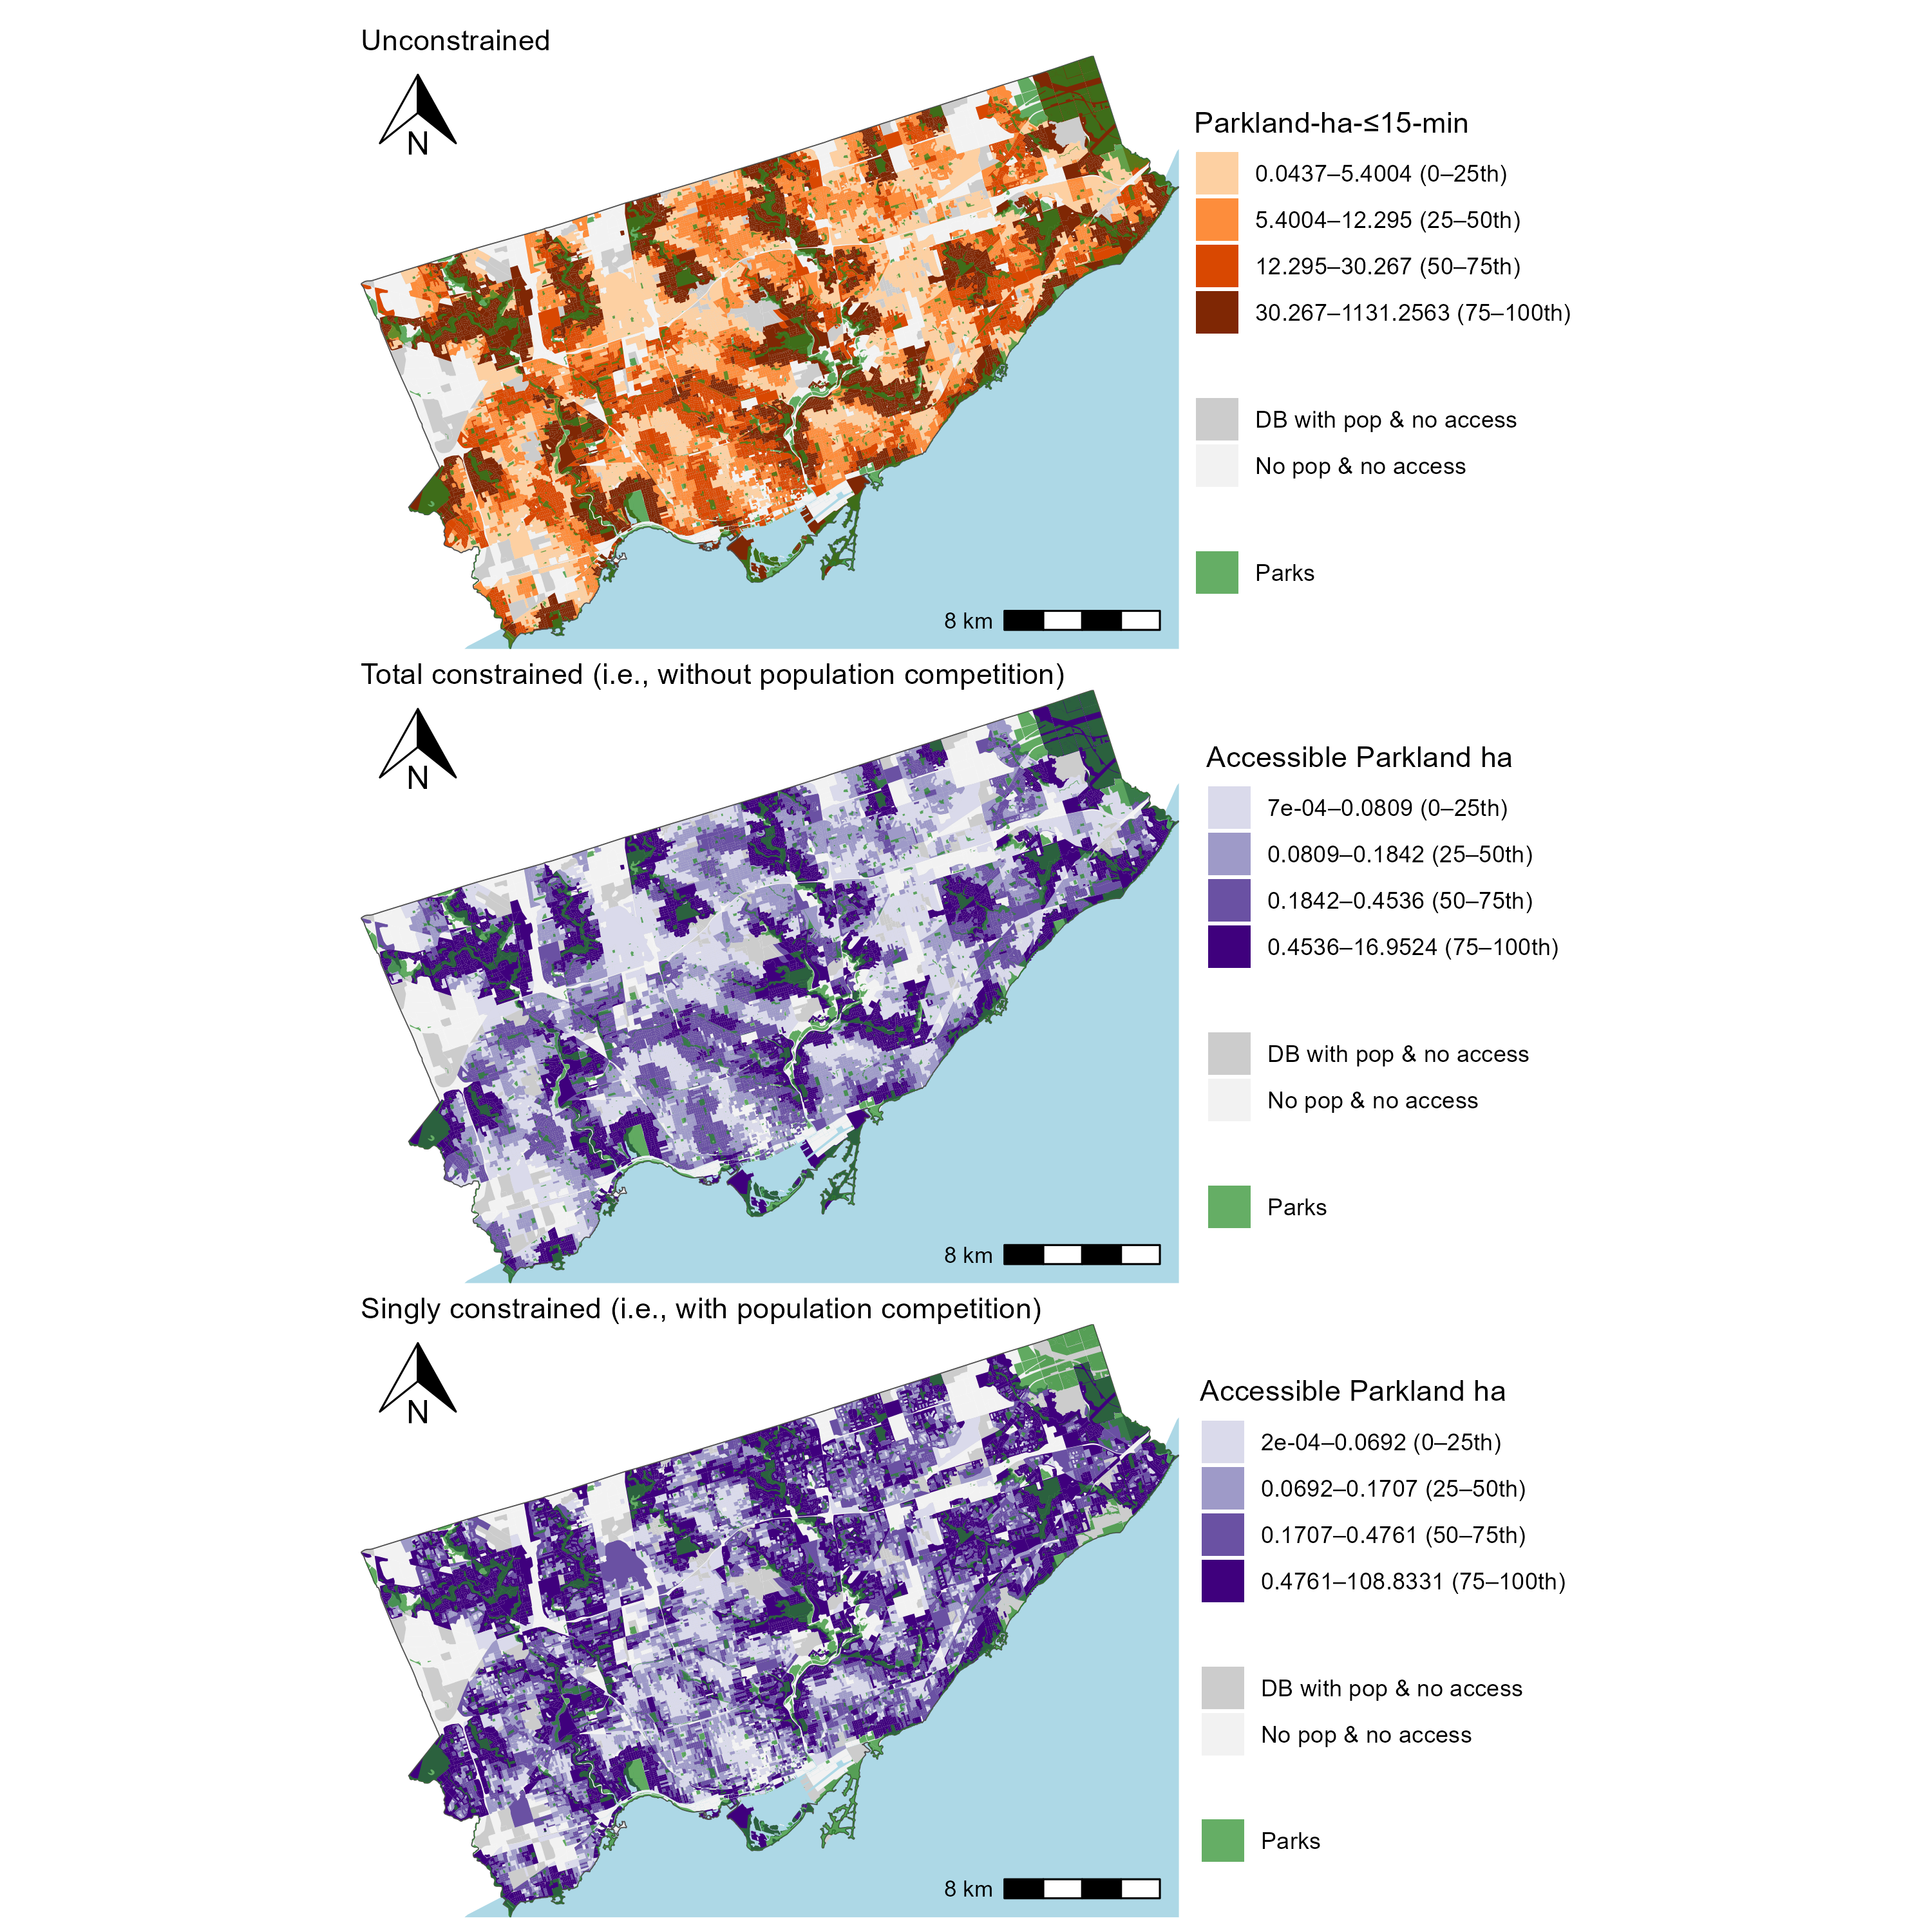
\includegraphics[width=6in]{./data/figures/chp4-parkland_access_DB_WALK_plots} 

}

\caption{\label{fig:chp4-parkland_access_DB_WALK_plots}Accessibility to parkland area per DB in Toronto.}\label{fig:unnamed-chunk-55}
\end{figure}

Also in Figure \ref{fig:chp4-parkland_access_DB_WALK_plots}, the total and singly constrained maps are shown in purple, reflecting constrained values (i.e., units of accessible parkland area). Their quartile bins are similar in magnitude, whereas the unconstrained plot's quartiles are not nor are the units comparable (representing units of parkland-ha-\(\le\)-15-minutes, a product of opportunity and impedance function). Within a 15 minute walk, only \(7632.922\) hectares of Toronto's total \(8037.547\) hectares of parkland (i.e., 95\%) are reachable and end up being included in the accessibility calculations. Accordingly, the sums of the constrained accessibility measures across all DBs equals 7632.922 hectares. The parks that remain inaccessible vary in classification and assumed entrance type (centroid or edge). The characteristics of these unreachable parks are discussed further in the following subsection on the \textbf{accessible population to parkland} in Section \ref{sec:accessible-pop}.

Across all plots in Figure \ref{fig:chp4-parkland_access_DB_WALK_plots}, DBs with no accessibility (i.e., light grey and grey) are represented. These areas correspond to the airport lands (Pearson airport) in the northwest; large indoor mall (Sherway Gardens) and the surrounding industrial and rail yard in the southwest; and natural areas in the northeast, including Rouge National Urban Park and the area surrounding Toronto Zoo, where protected lands, restrictive zoning, and steep terrain may limit development. Similar conditions are present in the city's centre near the Don Valley and associated river system, where floodplains and protected natural space restrict residential development.

Moreover, the total constrained plot in Figure \ref{fig:chp4-parkland_access_DB_WALK_plots} is proportional to the unconstrained plot by \(K^T\). As reviewed in Chapter 3, mathematically \(K^T\) is the sum of parkland area that can be walked to within 15 minutes (in ha) divided by the sum of total unconstrained accessibility in the city (\(\frac{7632.922}{509354.5} = 0.01498548\)). In this way, the total constrained plot can be similarly interpreted as the unconstrained plot (i.e.,15-minute cumulative opportunities measure) but in meaningful units: each DB's value now represents the amount of parkland area that can be accessed (out of the total parkland area). Because the total constrained measure is directly proportional to the unconstrained accessibility measure, areas of high and low access follow the same spatial pattern across both plots. Since a 15-minute walk radius covers only a limited distance beyond a park, it can be noted that DBs located within or adjacent to large parks appear in the top accessibility quartile, while those near smaller parks fall into the lower quartiles. In this way, the spatial pattern of the total constrained measure largely reflects the distribution and size of the parks themselves.

Further inspecting Figure \ref{fig:chp4-parkland_access_DB_WALK_plots}, the singly constrained plot contains 1.05 times more DBs with no accessibility than the constrained plot (1865 DBs have no accessibility instead of out of 1773 DBs out of the total 13322 DBs in the city). The singly constrained measure accounts for both reachability (travel impedance) \emph{and} population demand, so this measure yields zero accessibility for a DB containing no population but that still may be within a 15-minute walking distance of a park. Like the total constrained map, the singly constrained plot can be interpreted as a spatial diffusion of parkland, but one that reflects both travel impedance \emph{and} population demand.

As both the total and singly constrained measures use the same set and distribution of opportunities and travel impedance functions, they share similar spatial patterns in Figure \ref{fig:chp4-parkland_access_DB_WALK_plots}. However, they are still meaningfully diverge on account of population competition (i.e., a Pearson correlation of only 0.5795688. As the singly constrained measure considers population demand, DBs with a relatively high population within a 15-minute walking proximity to parks \emph{always} have high singly constrained accessible parkland, whereas this occurrence is only coincidental for the total constrained measure as population is not an input variable. Figure \ref{fig:chp4-singly_total_by_pop_heatmap} reflects this relationship between total constrained, singly constrained and this third variable: population.

\begin{figure}

{\centering 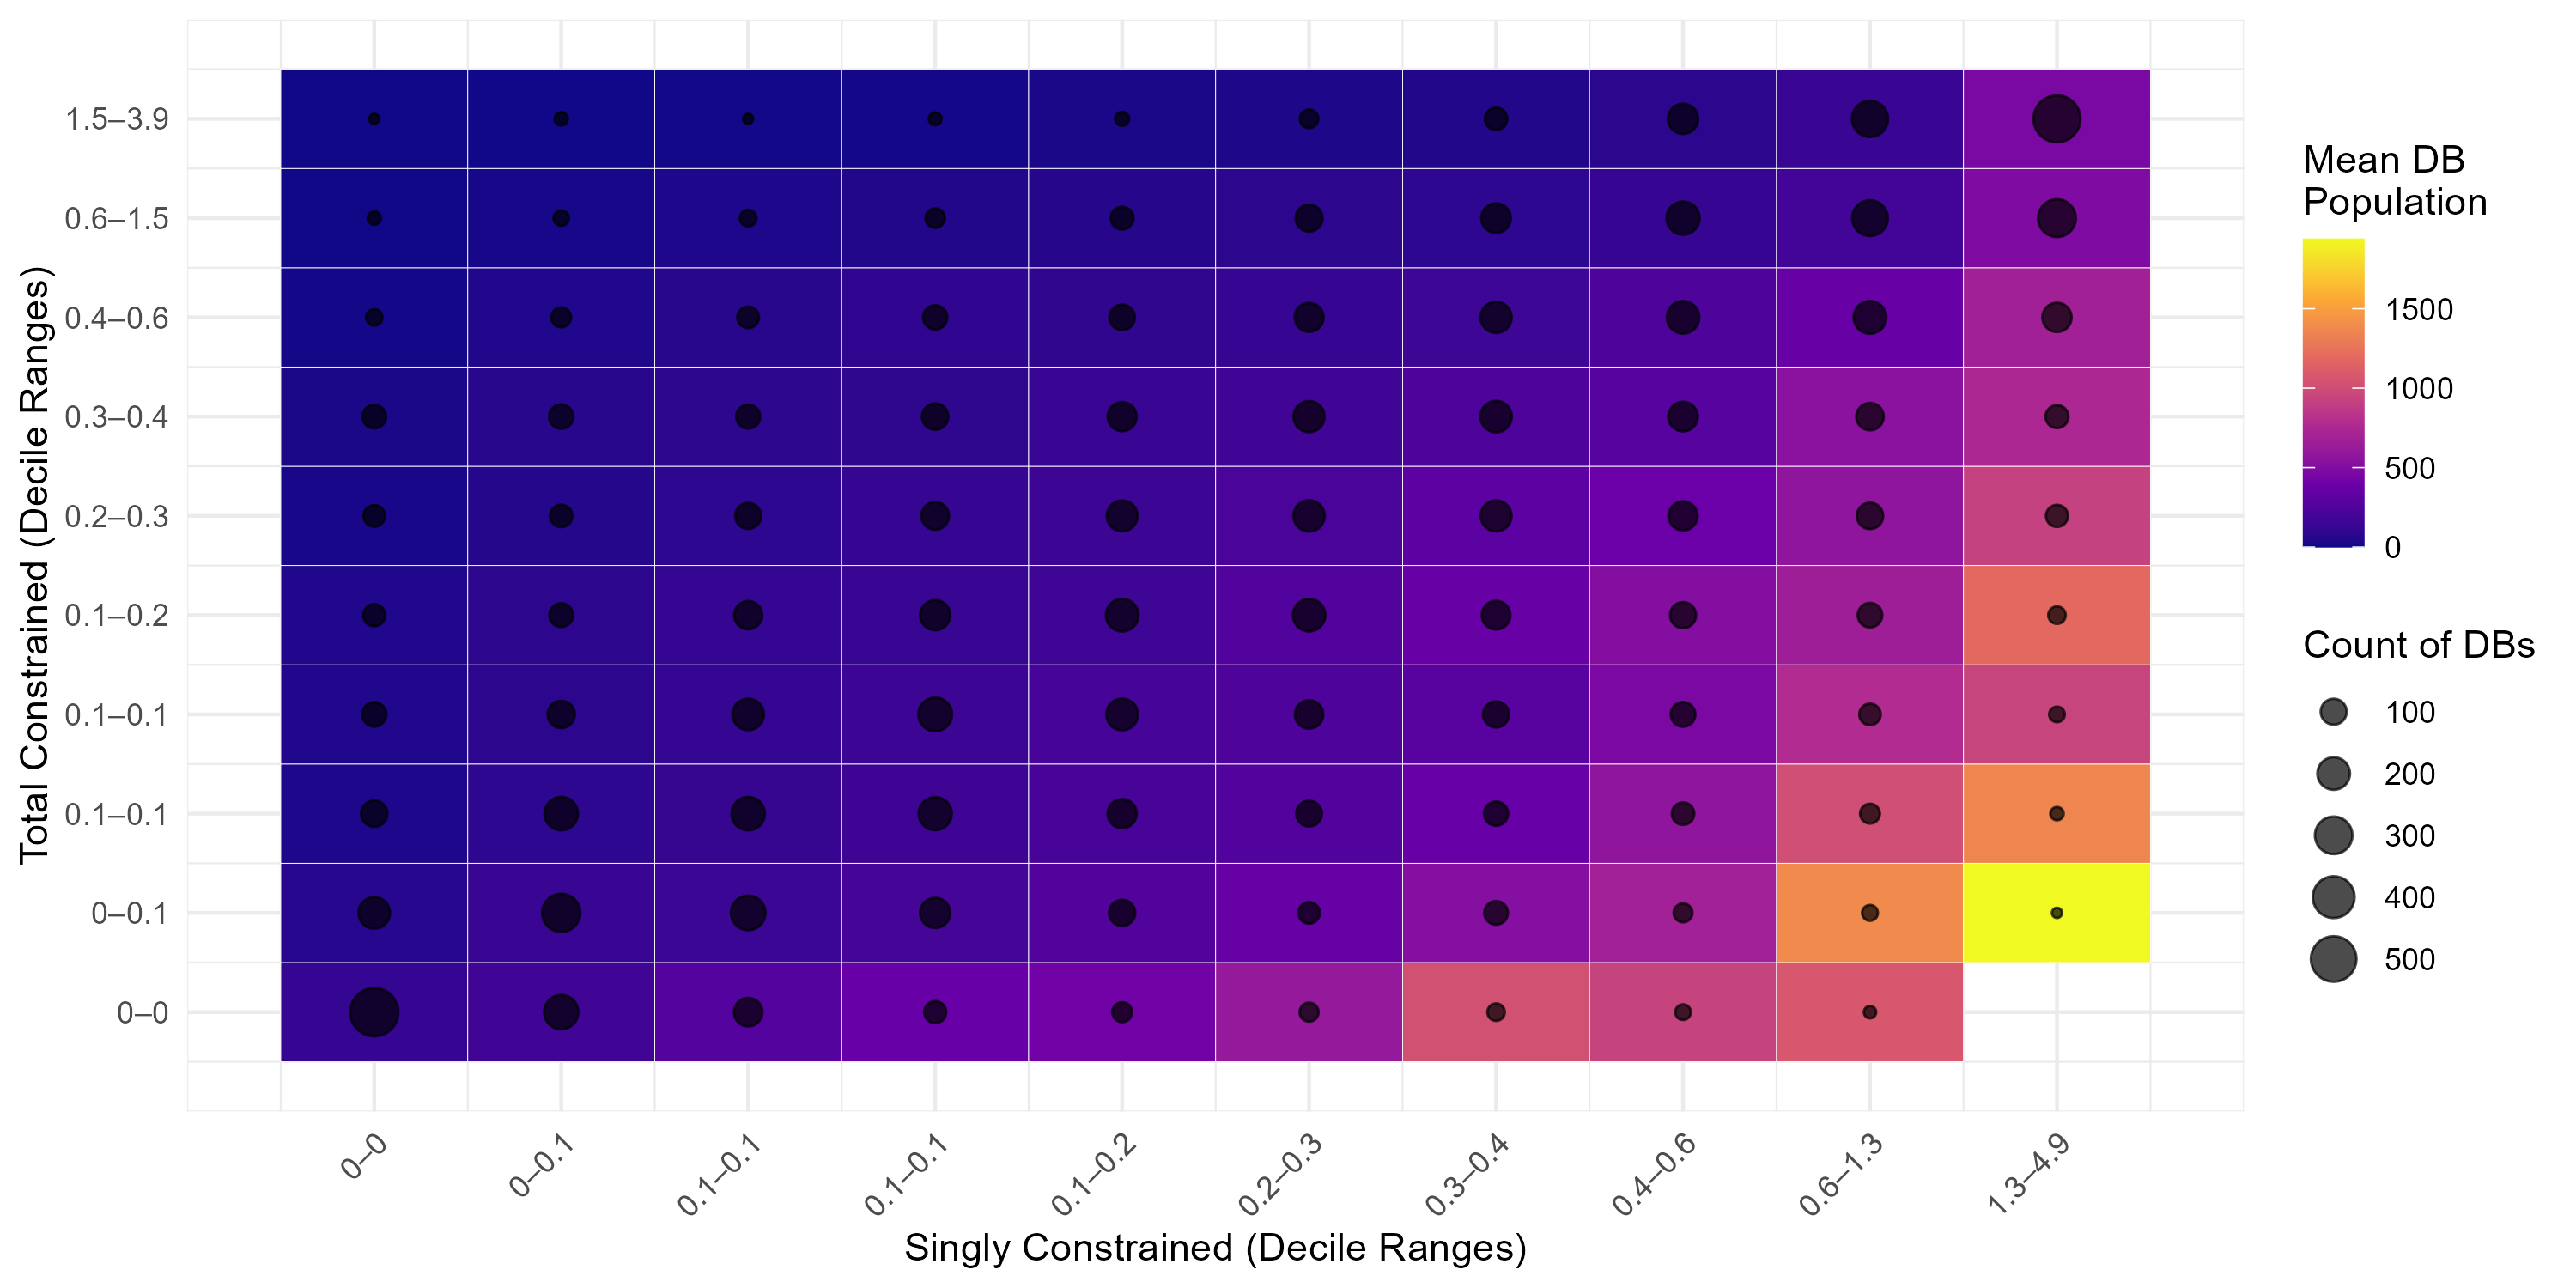
\includegraphics[width=6in]{./data/figures/chp4-singly_total_by_pop_heatmap} 

}

\caption{\label{fig:chp4-singly_total_by_pop_heatmap}Heatmap of DB-level mean population per deciles, total constrained accessible parkland area deciles and singly constrained accessible parkland area deciles.}\label{fig:unnamed-chunk-56}
\end{figure}

Regarding DBs with high and low population in Figure \ref{fig:chp4-singly_total_by_pop_heatmap}. Notably, DBs with high singly constrained values and low total constrained values always have above average population (i.e., pinks, above 500 people per DB). Conversely, DBs with low singly constrained values always have low average population but can have any range of total constrained values. In this way, considering population competition introduces more variation in the results. Compared to the total constrained values, the singly constrained values are more often zero, and tend to be lower (median is 0.17 for singly constrained and 0.18 for total constrained) or higher (Q3 and max value of 0.48 and 108.83 for singly constrained vs.~0.45 and 16.95 for total constrained).

Furthermore: the single constraint functions at a different scale than the total constraint. It allocates the area of each park to DBs that can reach it within 15 minutes, whereas the total constraint simply allocates the total parkland area, irrespective of the amount of area of the individual parks as long as the total constraint is satisfied.

This dynamic can be observed just west from the center of the city near the shoreline in Figure \ref{fig:chp4-parkland_access_DB_WALK_plots} where the area is both relatively dense in population and well-served by smaller to medium sized parkland. As a result, it shows lower singly constrained accessibility values compared to total constrained values reflecting the adjustment for population demand.Put another way, areas over-allocated parkland area than what the population demands when refering to the total constrained measure. In contrast, further east along the shoreline, the population density is lower and the areas are rich in parkland area. These areas consequently exhibit higher singly constrained than total constrained values. Because population is low and green space is abundant, these areas can be seen to have under-allocated parkland relative to their population demand.

The over- and under- allocation of parkland area is another way to discuss the difference between singly and total constrained accessibility. In Figure \ref{fig:chp4-singly_total_by_parksize_scatter}, the sum of \(V_{ij}^S\) and \(V_{ij}^T\) flows from each park are calculated and plotted against one another. Recall that the sum of singly constrained flows to a park is equal to its actual area, since the singly constrained factor proportionally allocates only the park's land area to reachable origins. This plot therefore illustrates how the total constrained measure allocates parkland area compared to a park's actual area. Parks plotted above the red 1:1 line allocate more accessible parkland than their actual area--indicating these parks are more centrally located or more accessible within the region. Parks below the line allocate less accessible area than they physically contain, suggesting they are more peripheral or less competitive. Interestingly, most parks fall below the line, under-allocating relative to their size. However, a small number--especially among the larger parks--allocate substantially more than their physical area.

\begin{figure}

{\centering 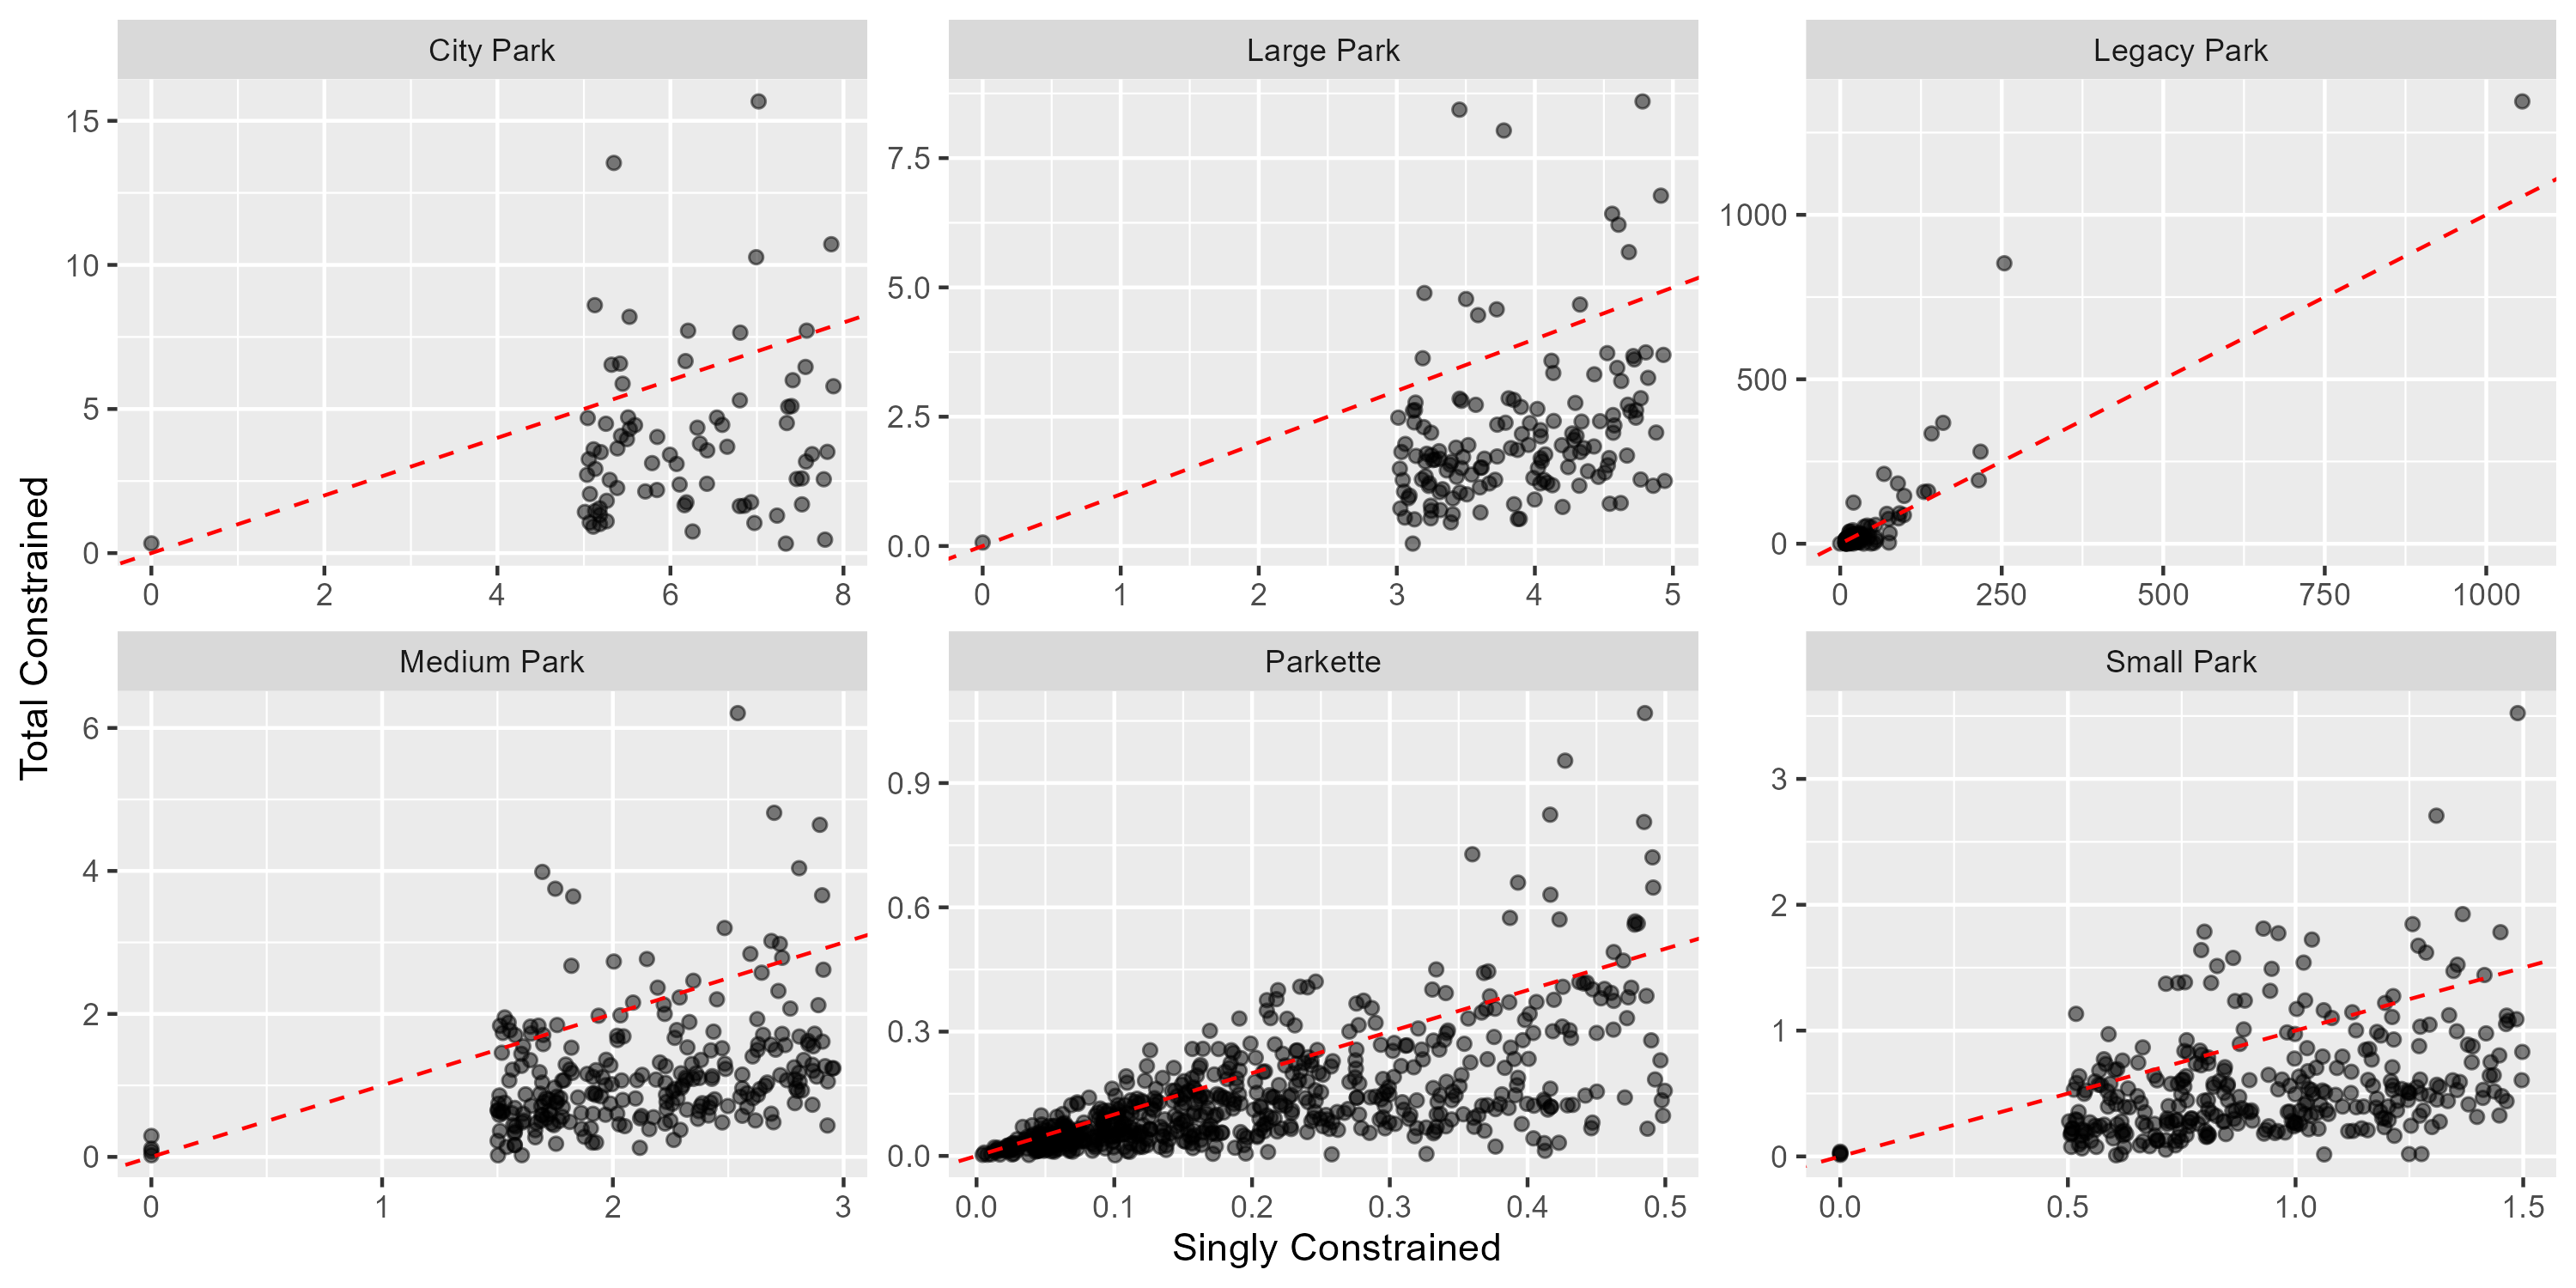
\includegraphics[width=6in]{./data/figures/chp4-singly_total_by_parksize_scatter} 

}

\caption{\label{fig:chp4-singly_total_by_parksize_scatter} Sum of constrained accessible parkland area flows from each park, reflecting the over and under allocation of total constrained accessible parkland area relative to actual parkland area (or singly constrained accessible parkland area). A plot for each park size classification.}\label{fig:unnamed-chunk-57}
\end{figure}

The top three such parks in each size category are labeled in Figure \ref{fig:chp4-singly_total_by_parksize_scatter}. These parks can be interpreted as having `over-allocated' parkland, due to high desirability (i.e.~demand by the origin mass) or centrality (i.e., low cost). In summary: parks above the line experience greater `spatial demand' than parks below the line. Hence, accessibility flows from parks above the line (and parks below the line) may be especially susceptible to change depending on the constrained accessibility measure used. In essence, centrally located parks over-allocate relative to their actual area, while peripheral parks under-allocate--an imbalance corrected when population demand is incorporated in the singly constrained measure.

In summary: both constrained measures offer more interpretable insights than unconstrained accessibility. The total constrained measure is similar in spirit to commonly used metrics like the 15-minute opportunity, but with a meaningful twist: its units can be interpreted as accessible parkland area (in hectares or any area unit). Furthermore, the total constrained accessibility measure also over- and under- allocates relative to the amount of parkland area actually available from a specific park, echoing the issue of `inflation' discussed in competitive accessibility literature (Antonio Paez et al., 2019; Soukhov et al., 2023). In contrast, the singly constrained measure also offers the same enhanced interpretation of resulting values being in units, as well as being a `competitive' accessibility measure. It incorporates both population demand and travel impedance, making allocation a function of both population demand for opportunities mediated by travel impedance as well as travel impedance to opportunities as the traditional unconstrained measure.

\subsection{Neighbourhood-level accessible parkland area}\label{neighbourhood-level-accessible-parkland-area}

Another way of examining the accessibility data is by aggregating it to a spatial zoning system with more meaning for policy: such as the neighbourhood. These areas are City-designated `social planning neighbourhoods' which are used by staff to collect data, plan and analyse service provision (City of Toronto, 2024). Also each neighbourhood, as reviewed in Chapter 3, is labelled with either a Emerging Neighbourhood (EN), Neighbourhood Improvement Area (NIA), or neither classification; an additional dimension in determining if the area is should be prioritized or not from the point of equity. In the Figure \ref{fig:chp4-parkland_access_neighbourhood_WALK_plots}, all \(V^0_{ij}\), \(V^T_{ij}\) and \(V^S_{ij}\) values are summed and presented at this level of aggregation.

\begin{figure}

{\centering 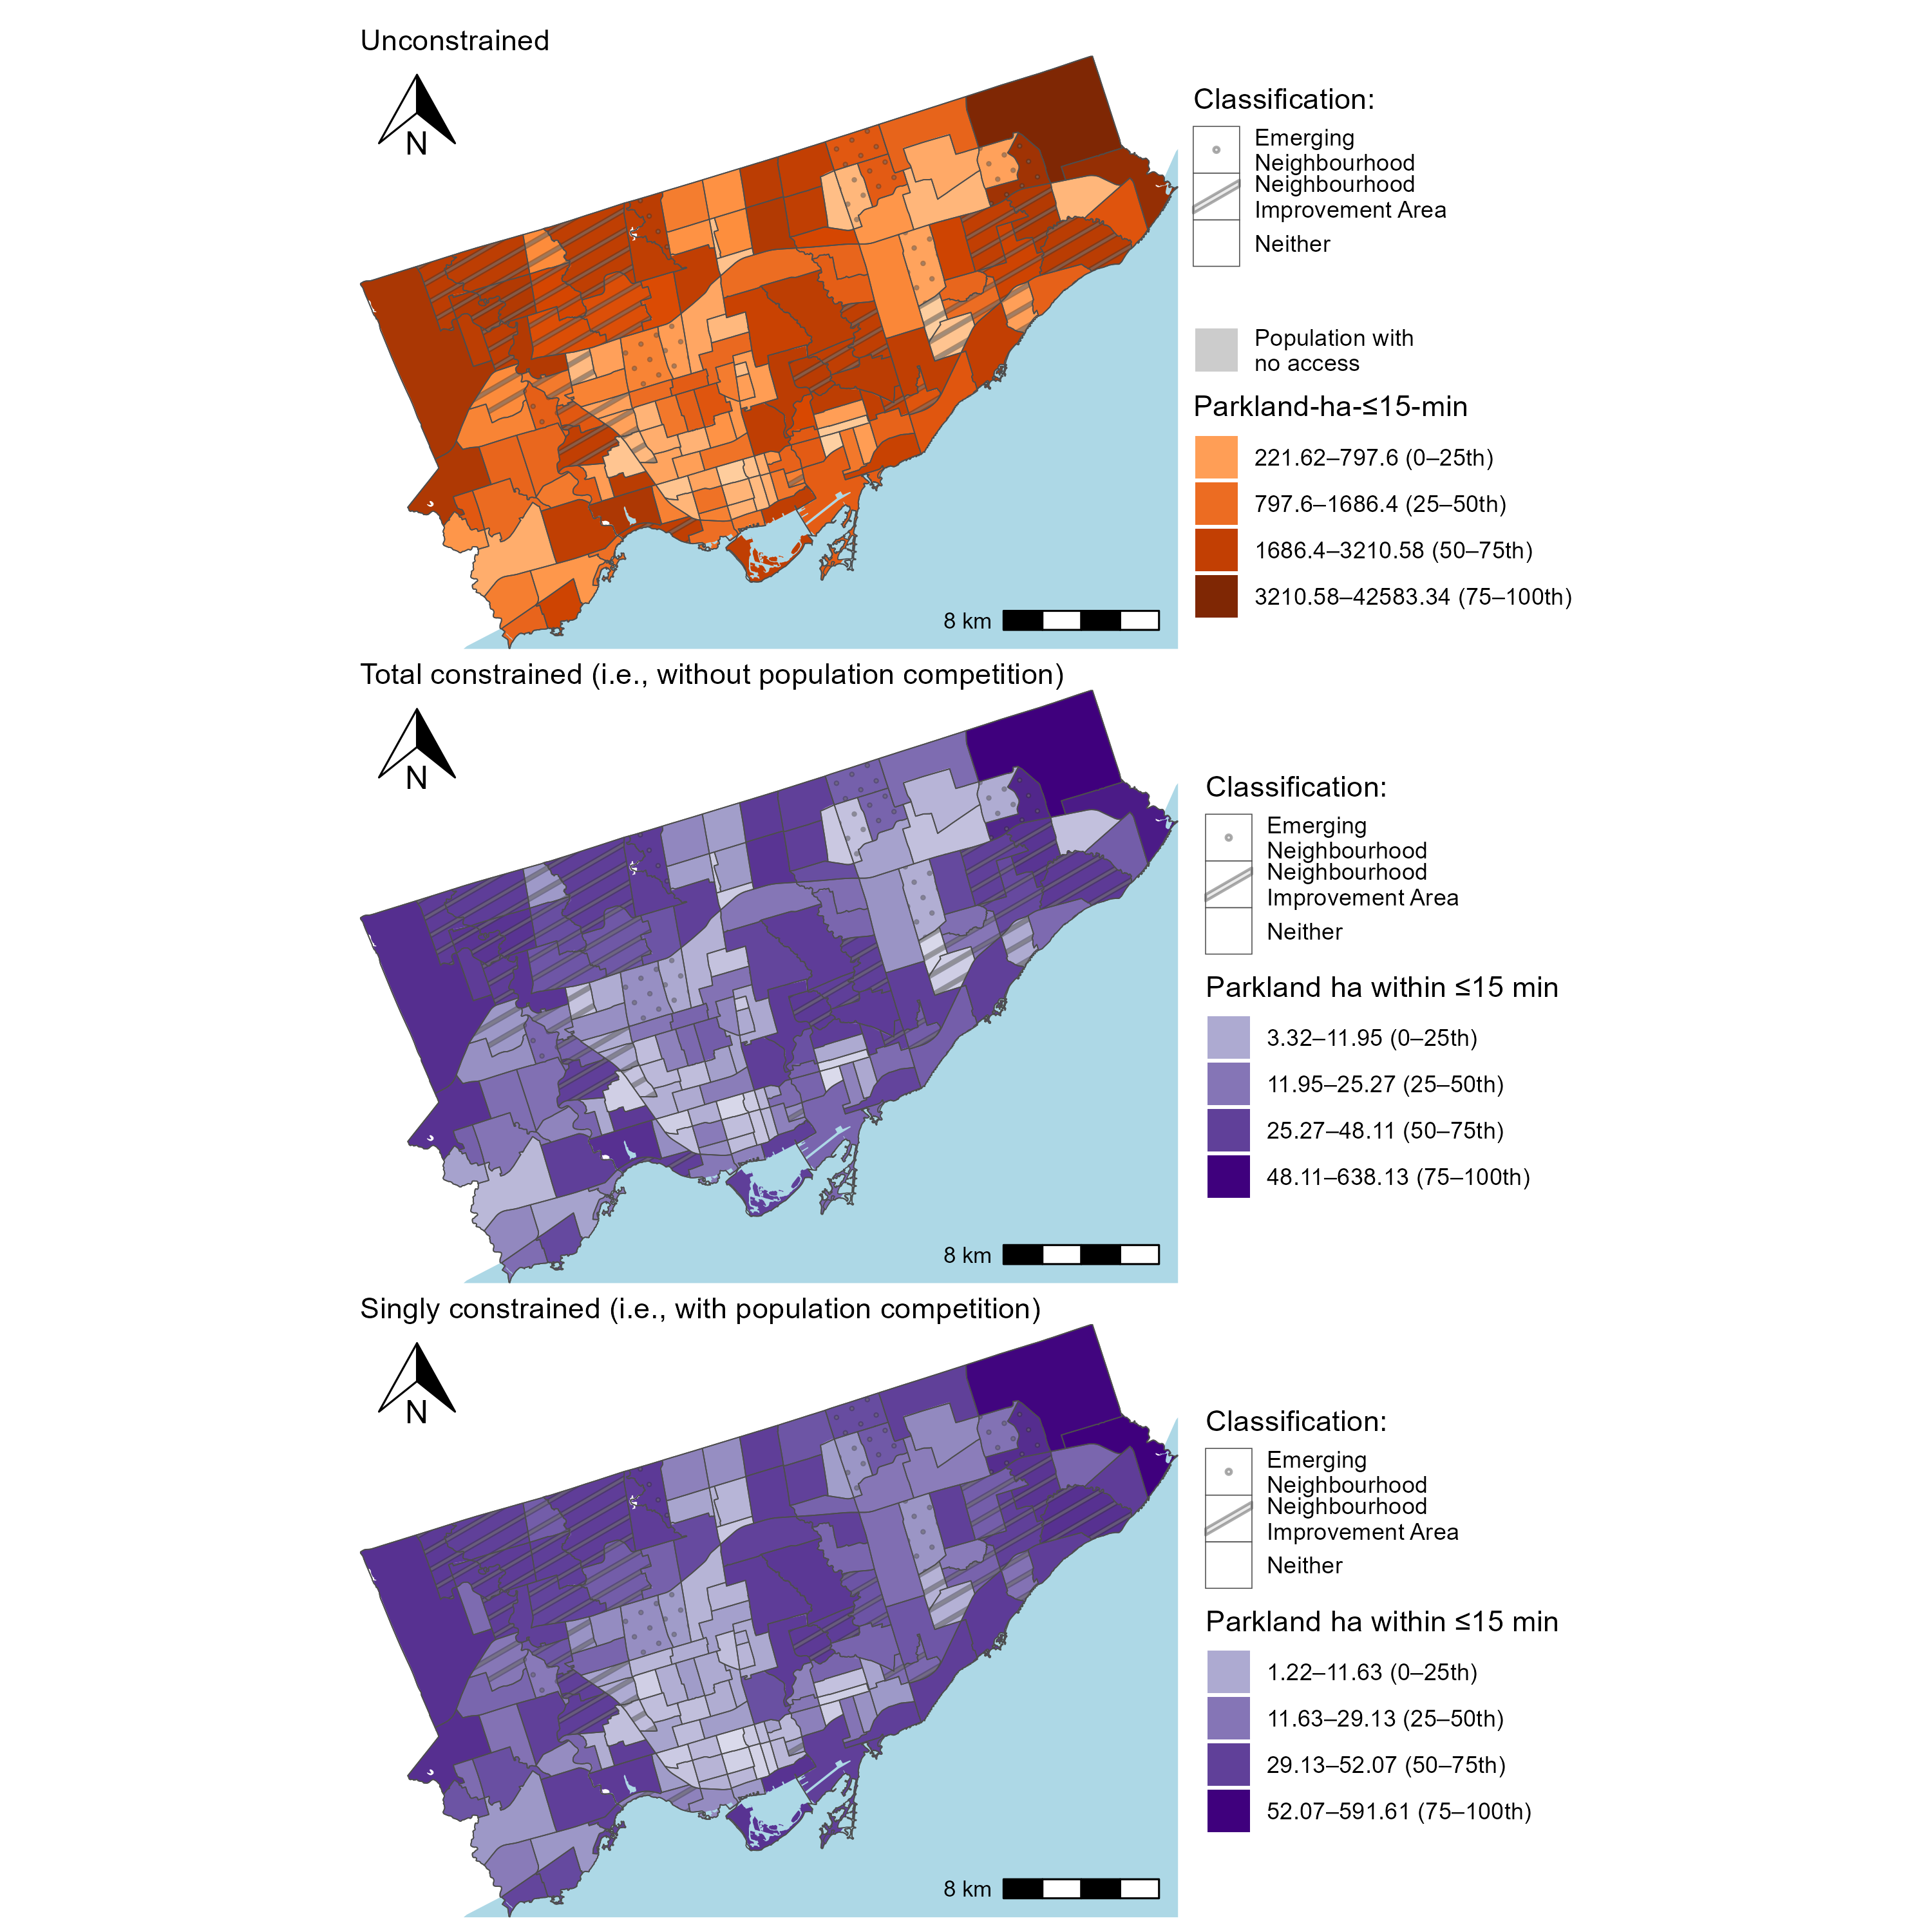
\includegraphics[width=6in]{./data/figures/chp4-parkland_access_neighbourhood_WALK_plots} 

}

\caption{\label{fig:chp4-parkland_access_neighbourhood_WALK_plots}Acessibility to parkland area per neighbourhood and neighbourhood classification in the city of Toronto.}\label{fig:unnamed-chunk-58}
\end{figure}

In Figure \ref{fig:chp4-parkland_access_neighbourhood_WALK_plots}, the unconstrained values are not fixed to any meaningful zonal or regional total whereas the sum of total constrained and singly constrained values equal to all the amount of parkland area in the city. For instance, in the top quantile, dark oranges represent 2737 `parkland-ha-\(\le\)-15-min' or greater, now summed at the area of the neighbourhood. Whereas the top quantile in the total constrained measure represent the 41 ha or greater that is accessible, directly in units of parkland area that can be accessed out of the total parkland hectares. Summing all DBs within a neighbourhood maintains this total constraint and hence this associated intuition.

The same logic can be applied to the singly constrained measure, but with the additional consideration of population competition. And like Figure \ref{fig:chp4-parkland_access_DB_WALK_plots}, values between the measures in Figure \ref{fig:chp4-parkland_access_neighbourhood_WALK_plots} share some commonalities: unconstrained and total constrained measures still remain proportional (by \(K^T\)), and the singly constrained values match total constrained values in DBs with and near population values that are relatively average. Singly constrained values deviate when population is low (i.e., singly constrained values are lower than total constrained) and population is high (i.e., singly constrained values are higher than total constrained values). If the heatmap of these two measures and population was reproduced at the neighbourhood aggregation, the general trends would be similar as at the DB level.

However, the trends in the data are smoothed in this aggregation as shown in the density distribution plots of the constrained measures under the different aggregations in Figure \ref{fig:chp4-dist_db_vs_neigh_plots}. At both the DB and neighbourhood levels, the total constrained accessibility distribution is right-shifted and more dispersed compared to the singly constrained measure. This indicates that parkland is allocated more evenly under the total constraint, with fewer areas experiencing extremely high or low access. In contrast, the singly constrained measure shows a slightly more peaked and skewed distribution, reflecting localized competition for limited park space. At the DB-level, accessibility measures are more granular and variable, capturing finer differences in proximity and population competition. This results in a wider range and more extreme values, especially under the singly constrained measure, which reflects localized demand. At the neighbourhood-level, aggregating across DBs smooths out some of the variation and reduces some extremes. While this can enhance interpretability at a policy scale, it may also mask pockets of low or high access that could be critical. For this reason, examining patterns at the lowest level of aggregation should be considered best practice, alongside summing to zoning systems that have more significant meaning from a planning perspective (such as Neighbourhood).

\begin{figure}

{\centering 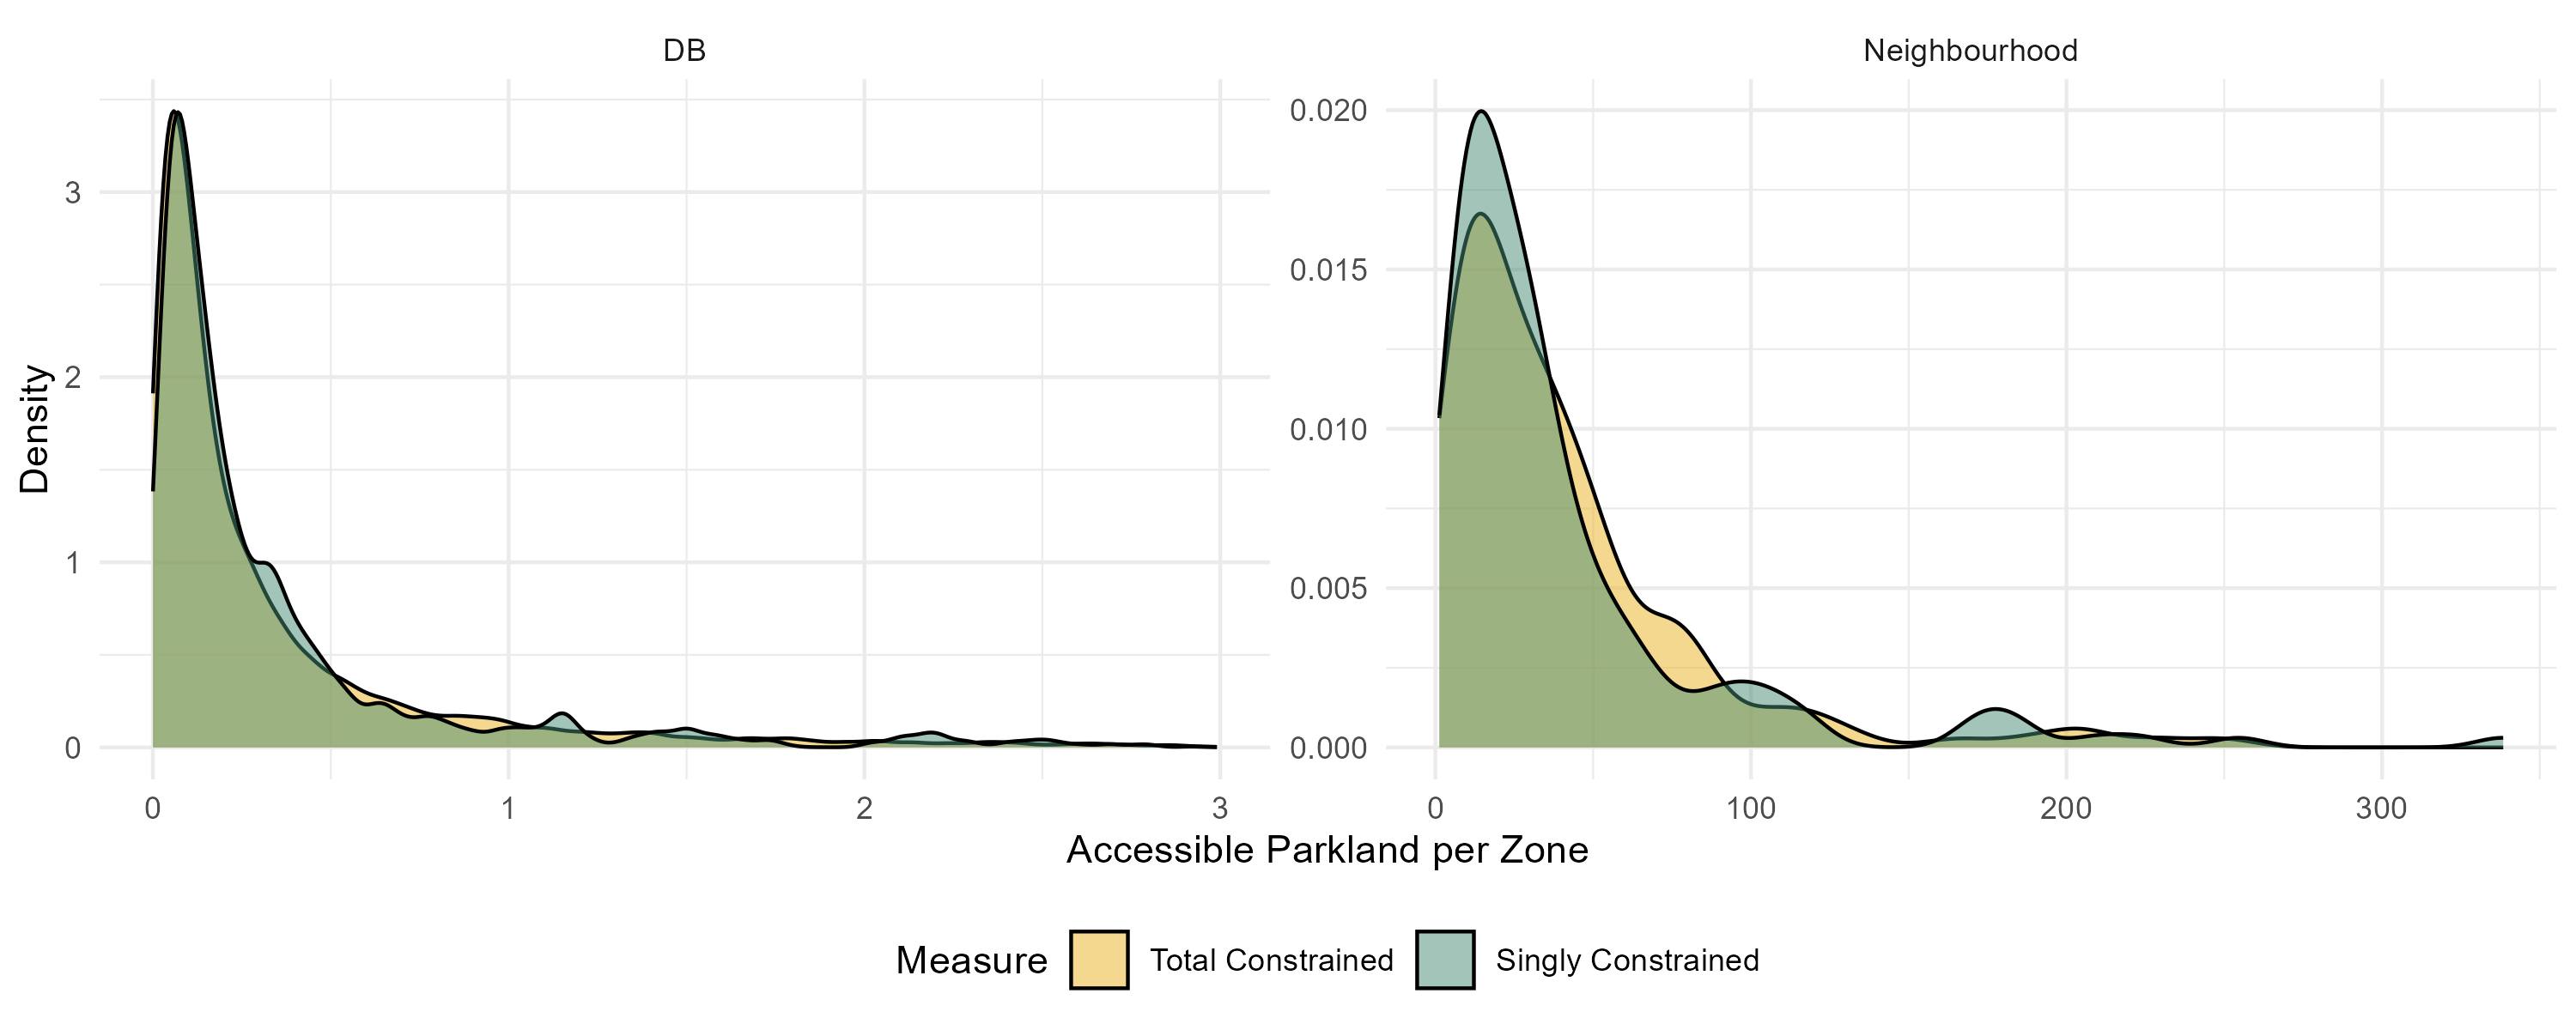
\includegraphics[width=6in]{./data/figures/chp4-dist_db_vs_neigh_plots} 

}

\caption{\label{fig:chp4-dist_db_vs_neigh_plots}Density distribution of the constrained accessibility measure values at the dissemination block and neighbourhood block. For both aggregations, the datasets are truncated at top decible for the purpose of visualisation.}\label{fig:unnamed-chunk-59}
\end{figure}

Furthermore: since DBs reflect the smallest units of population from the census (range between 0 to 3375, median of 117 people), much smaller than the city-designed neighbourhoods (which range between 6419 to 33690, median of 17024 people), the following question may arise specifically for neighbourhoods: what is the accessible parkland ha per neighbourhood population? This per capita measure is visualised in Figure \ref{fig:chp4-parkland_access_neighbourhood_percapita_WALK_plots}.

\begin{figure}

{\centering 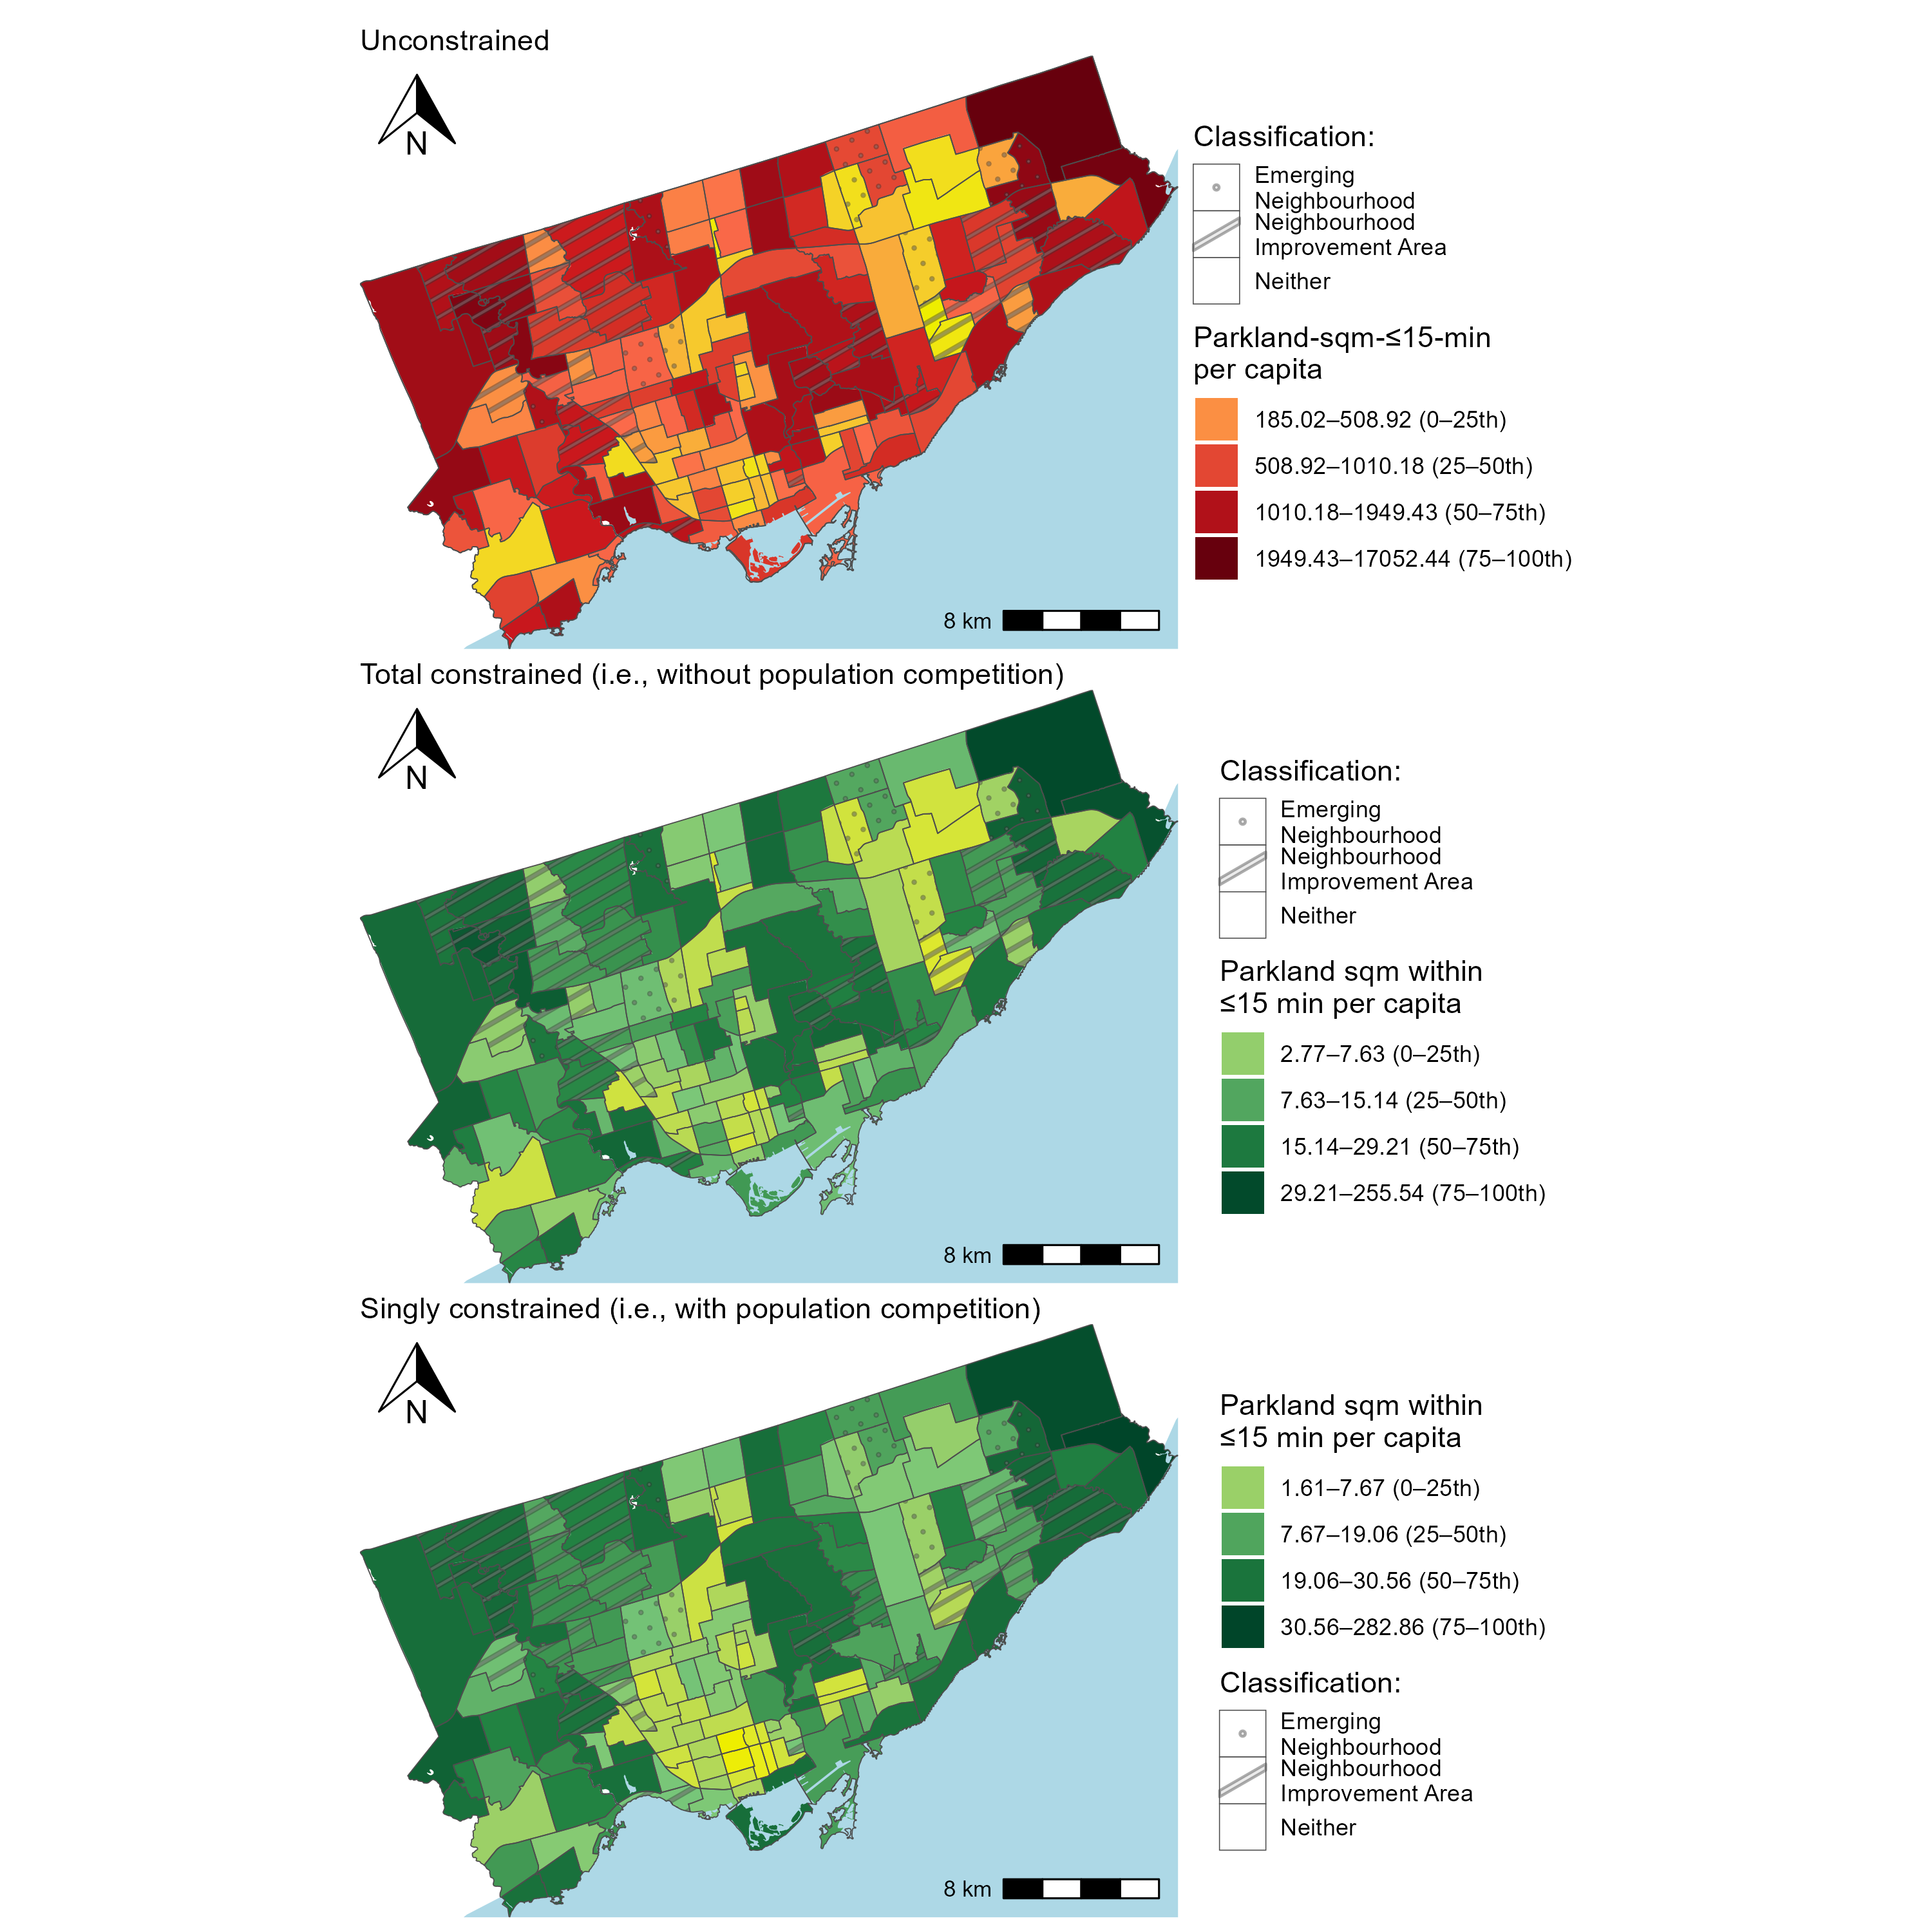
\includegraphics[width=6in]{./data/figures/chp4-parkland_access_neighbourhood_percapita_WALK_plots} 

}

\caption{\label{fig:chp4-parkland_access_neighbourhood_percapita_WALK_plots}Map of Toronto CMA with accessibility to parklands per neighbourhood and neighbourhood classification}\label{fig:unnamed-chunk-60}
\end{figure}

In Figure \ref{fig:chp4-parkland_access_neighbourhood_percapita_WALK_plots}, all three accessibility measures are shown, though the unconstrained measure should be interpreted with caution. Since the unconstrained measure lacks a constraint, the units--parkland-hectares\(\le\)-15-minute' divided by neighbourhood population--are more complex to decipher. While neighbourhood population is a fixed and tangible quantity (i.e., a known share of the total population), the amount of `parkland-hectares\(\le\)-15-minute' is not similarly bounded or consistently defined across the region. Hence, for a non-competitive yet interpretable alternative to the unconstrained measure, the per capita total constrained accessibility (second plot in Figure \ref{fig:chp4-parkland_access_neighbourhood_percapita_WALK_plots}) should be considered, as it retains intuitive units while incorporating the intuition of the unconstrained measure.

For the constrained measures in Figure \ref{fig:chp4-parkland_access_neighbourhood_percapita_WALK_plots}, park supply categories from the Toronto Parkland Report (City of Toronto, 2019) are used for the scale. This report quantifies the amount of parkland area into meaningful human-scaled bins: the area within a hula hoop (2 sqm), the space beneath a patio umbrella (4 sqm), the space within a bus shelter (12 sqm), and the canopy of a mid-size tree (28 sqm+). Figure \ref{fig:chp4-parkland_access_neighbourhood_percapita_WALK_plots} uses these relatable labels for accessible per capita parkland area, applied to constrained measures.

The interquartile ranges of both constrained measures in Figure \ref{fig:chp4-parkland_access_neighbourhood_percapita_WALK_plots} correspond to the relatable bins, ranging between the area of a patio umbrella and a tree canopy, with medians just above the space of a bus shelter. Specifically: the total constrained accessibility interquartile range is 6.9 to 26 accessible sqm of parkland per capita with a median of 13 sqm per parkland per capita. The singly constrained accessibility score's interquartile range is 7.6 to 30.6, with a median of 18.7 sqm of parkland per capita. No neighbourhood has 0 accessible parkland area.

In Figure \ref{fig:chp4-parkland_access_neighbourhood_percapita_WALK_plots}, as previously noted, the singly constrained values are generally more dispersed than the total constrained values (i.e., tending to be both higher or lower), so a similar pattern is expected in the per capita scores. And this holds true: the spatial distribution of raw scores and per capita rates closely align. For example, both measures show lower values (oranges and reds) concentrated downtown and higher values (greens) in the centre part of the city near the Don Valley system. However, some areas diverge: along the shoreline east of downtown where residential density is lower but green space is plentiful, per capita scores are especially high for the singly constrained measure but only moderately high for the total constrained measure.

The discussion of how neighbourhoods change value depending on the measure used is important, as the purpose of aggregating the constrained measures at the neighbourhood level can be to identify priority areas. To use common terminology: this analysis considers NIA and EN labelled neighbourhoods as priority areas. Interestingly, observing Figure \ref{fig:chp4-parkland_access_neighbourhood_percapita_WALK_plots} however, not all NIA/EN are equal in terms of accessible parkspace; some have plenty of accessible per capita parkland area while others do not. Regarding parkland supply thresholds, the City of Toronto (2019) report selects the normative threshold of parkland area of 12 sqm (bus shelter) per capita as a value below that should be considered priority. And as an additional point of reference, this is slightly more than the 9 sqm per inhabitant recommended by the WHO (OECD, 2013). Hence, in this analysis, it is assumed then that neighbourhoods that are NIA/EN and contain below 12 sqm parkland area that is accessible per capita are priority neighbourhoods for incerased parkland area supply.

Using these two criteria and depending on which constrained per capita measure is used, either 4 or 11 of the 43 NIA/EN neighbourhoods (out of 158 neighbourhoods overall) fall below the 12 sqm threshold for accessible parkland area per capita. Overall, the competitive (singly constrained) measure tends to produce consistently higher per capita values than the total constrained measure, reflecting the effect of population demand. These patterns for NIA, EN and neither neighbourhood classification scores are summarized in the boxplots in Figure \ref{fig:chp4-parkland_access_neighbourhood_percapita_WALK_boxplots}.

\begin{figure}

{\centering 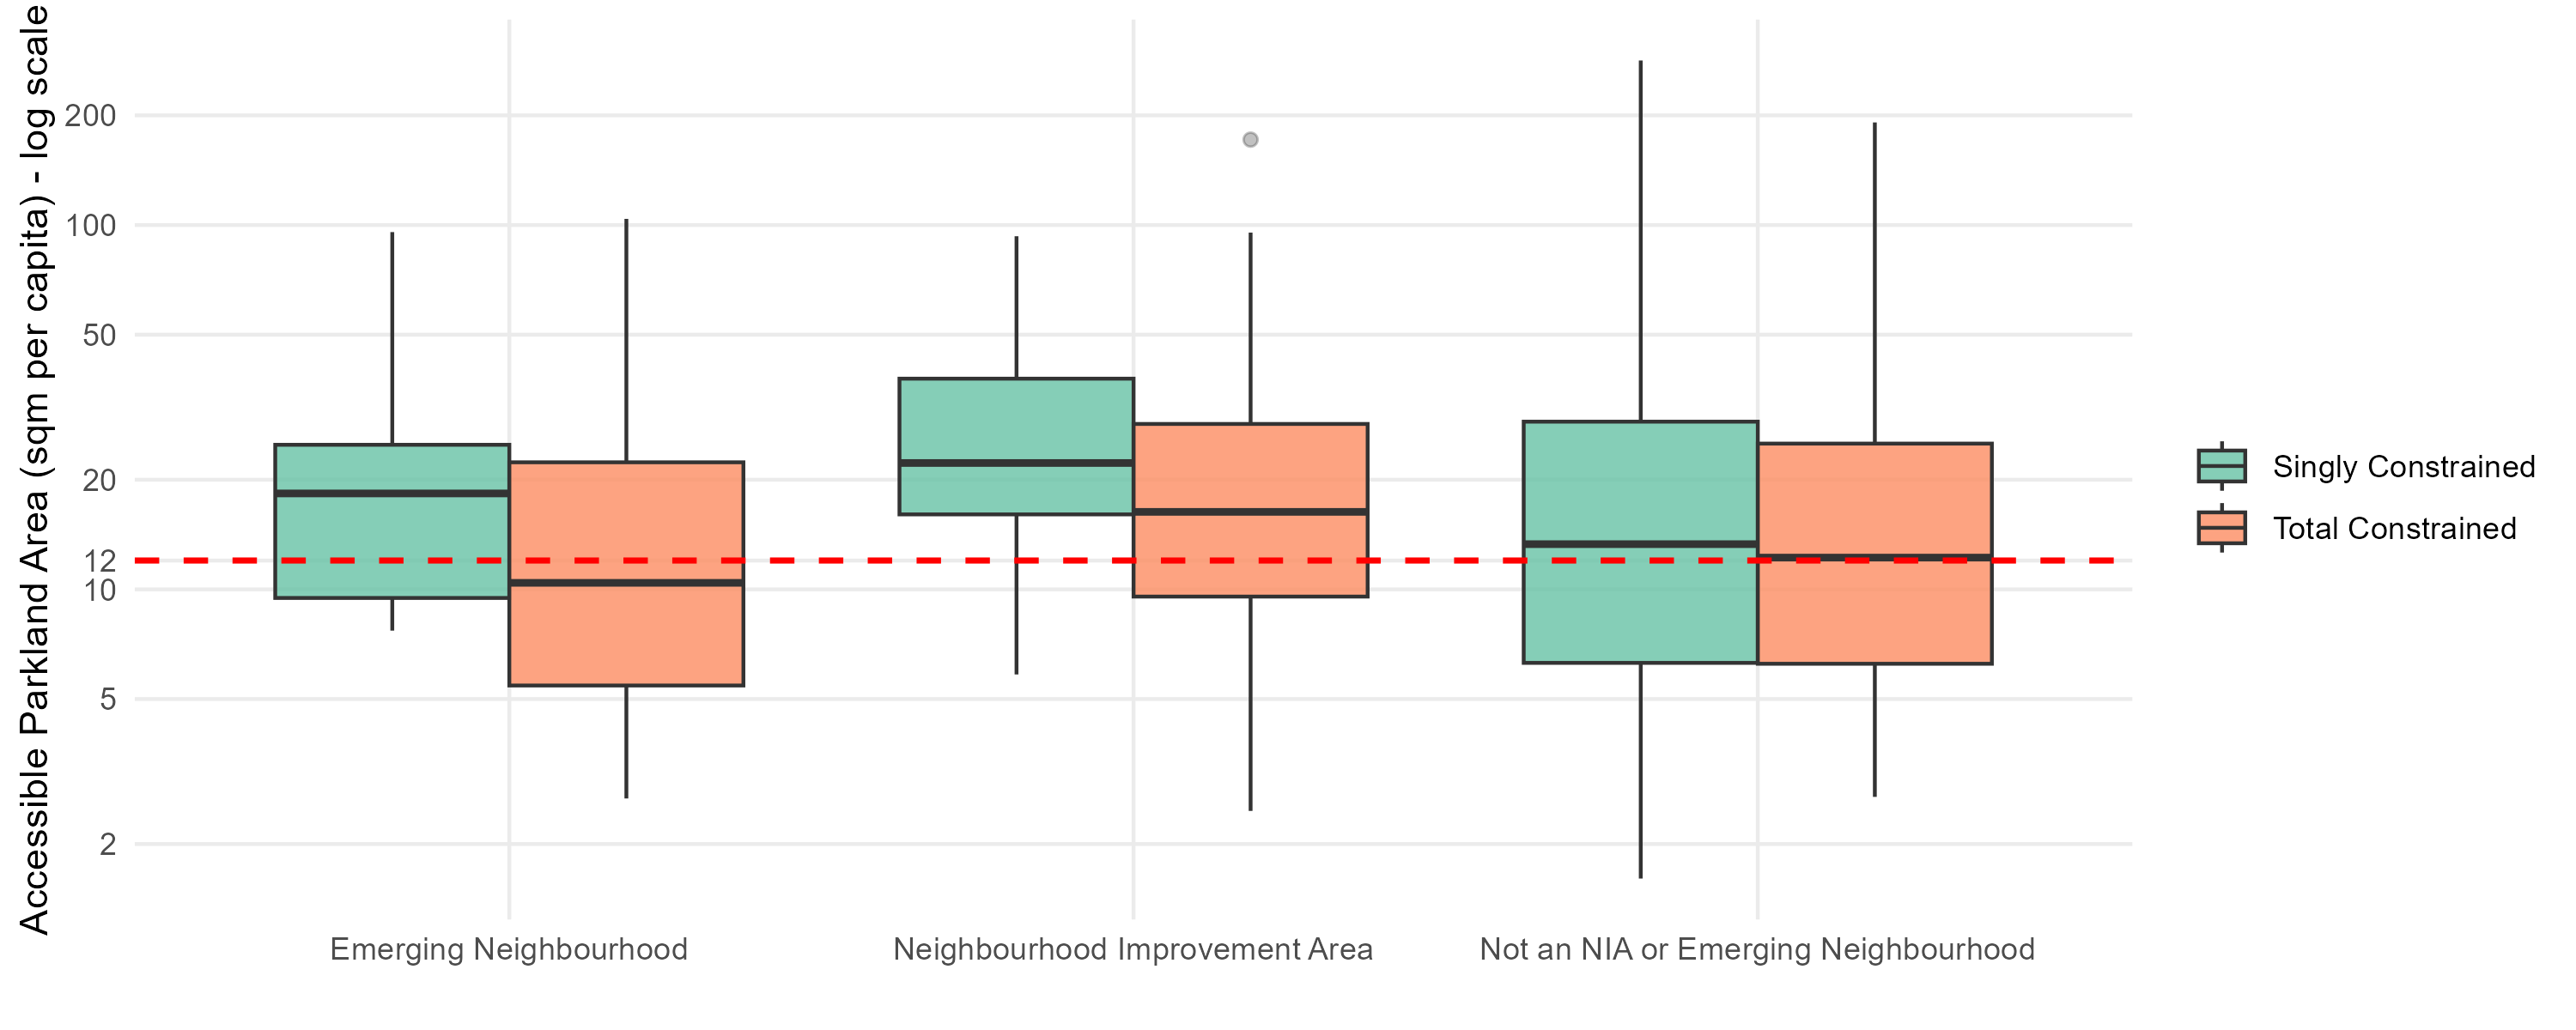
\includegraphics[width=6in]{./data/figures/chp4-parkland_access_neighbourhood_percapita_WALK_boxplots} 

}

\caption{\label{fig:chp4-parkland_access_neighbourhood_percapita_WALK_boxplots} Boxplot of singly constrained and total constrained per capita neighbourhood values summarised by type of neighbourhoof classification. }\label{fig:unnamed-chunk-62}
\end{figure}

From Figure \ref{fig:chp4-parkland_access_neighbourhood_percapita_WALK_boxplots}, it can be observed that the majority of NIAs have per capita scores above 12 sqm, especially when considering the singly constrained measure. However, some NIAs fall below this threshold under both measures--while others fall below only under the total constrained measure. The neighbourhoods below the threshold on both measures tend to be relatively dense (compared to other NIAs) and lack large parks, while those below only on the total constrained measure often contain large parks but only a portion of the population can access them. When population demand is considered (i.e., singly constrained) as the amount of area for the population is sufficiently high to exceed the threshold.

Also from Figure \ref{fig:chp4-parkland_access_neighbourhood_percapita_WALK_boxplots}, it can be observed that EN appear to diverge the most (relative to other neighbourhood classifications) depending on the measure used. No EN falls below the threshold for both measures, but four neighbourhoods fall below it when only the total constrained measure is considered. These neighbourhoods share similar characteristics with the NIAs that fall below the threshold considering the total constrained measure, i.e., large in area and only have a large park accessible to part of the neighbourhood population, which results in high total constrained access for that specific portion but low accessibility when aggregated across the entire neighbourhood. Conversely, when the (relatively) lower levels of population demand is considered in the singly constrained measure, singly constrained per capita scores exceed the threshold.

Lastly, gleaned from Figure \ref{fig:chp4-parkland_access_neighbourhood_percapita_WALK_boxplots}, neighbourhoods without either classification have median per capita scores close to 12 sqm, with singly constrained scores that are generally higher and more dispersed. Interestingly, the neighbourhoods with the lowest and highest per capita singly constrained scores tend to be in this group, located either west of the downtown core or along the shoreline as previously noted.

In summary, although some NIA and EN neighbourhoods do not meet the 12 sqm threshold, the majority exceed it under both constrained accessibility measures. This presents an optimistic outlook regarding accessible parkland area (as measured in this analysis) in the identified priority neighbourhoods.

Going beyond the NIA/EN classifications, another notable aspect of the difference in the total and singly constrained scores is its spatial distribution. How this difference results in a change of parkland area per capita category (i.e., 0-2, 2-4, 4-12, 12-28, or 28+ sqm per capita) is visualised in Figure \ref{fig:chp4-diff_singly_access_neighbourhood_parkland_percapita_WALK_plot}. While the choice of measure may not drastically impact the identification of NIA/EN neighbourhoods below the 12 sqm threshold (with exception of a few, as discussed), it does produce different results overall i.e., the range of difference in neighbourhood values are between -95.08 and 111.60 accessible parkland sqm per capita. This distinction could be important in other contexts and may influence policy decisions.

\begin{figure}

{\centering 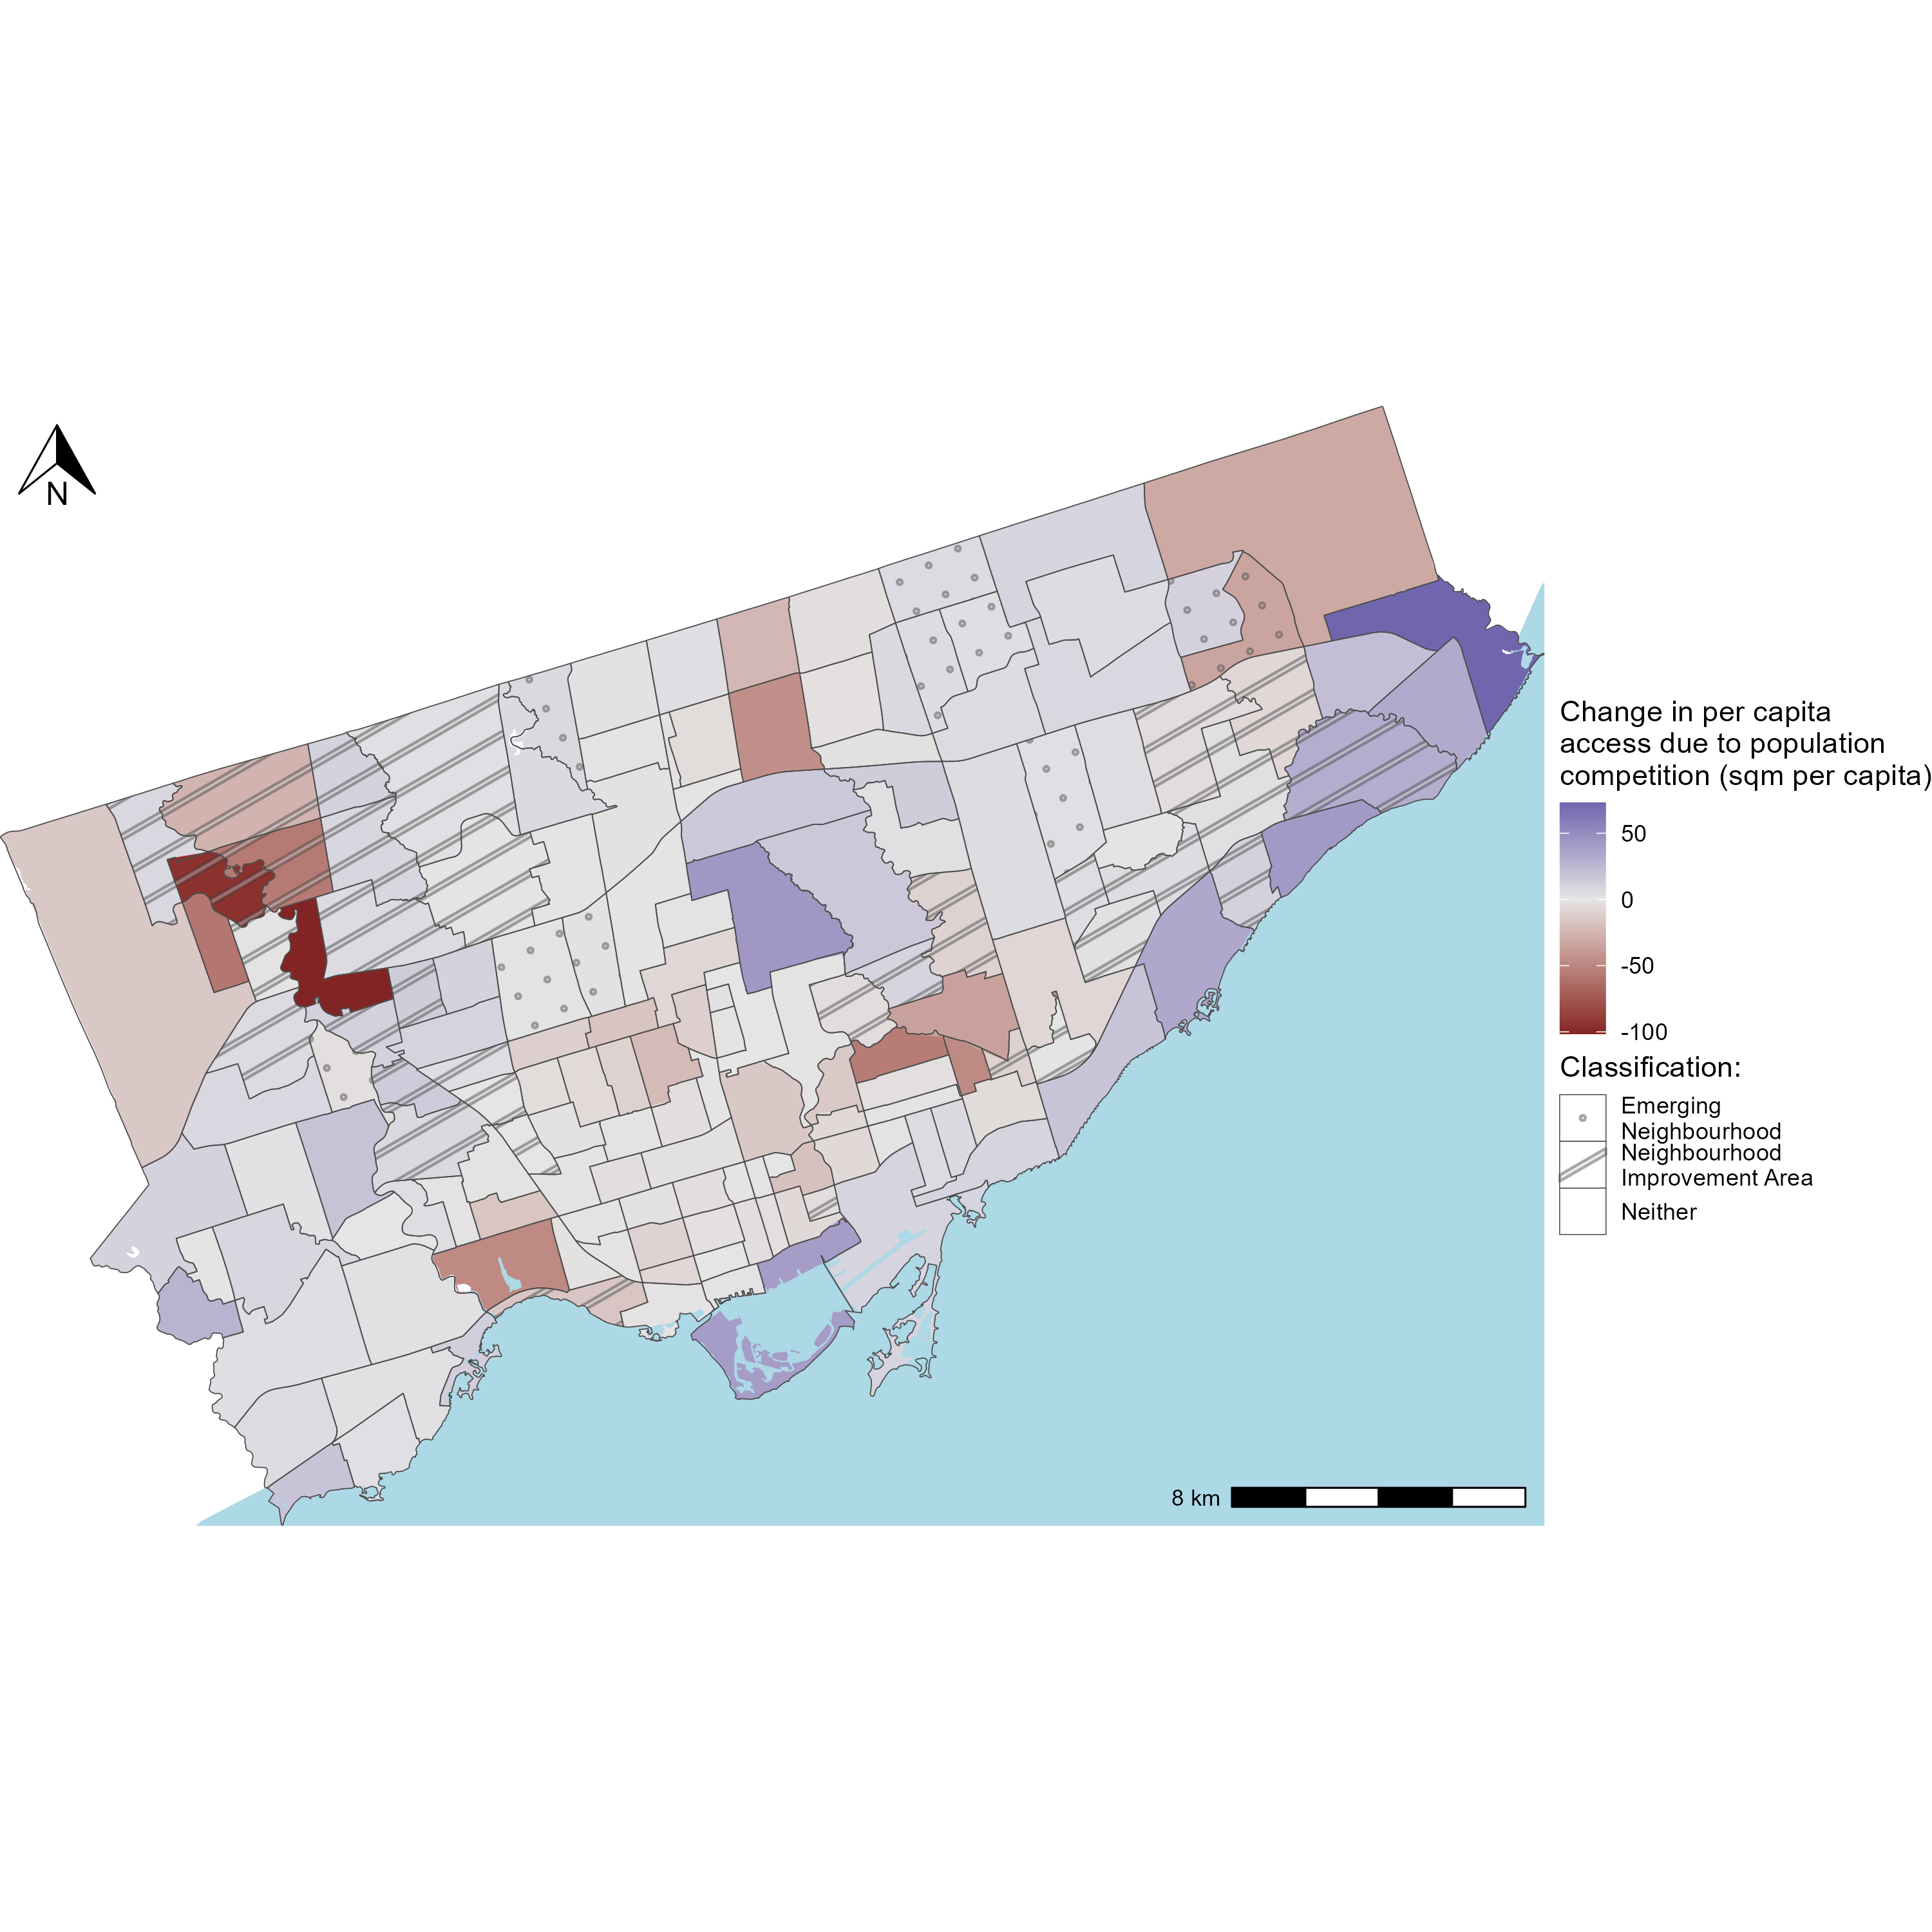
\includegraphics[width=6in]{./data/figures/chp4-diff_singly_access_neighbourhood_parkland_percapita_WALK_plot} 

}

\caption{\label{fig:chp4-diff_singly_access_neighbourhood_parkland_percapita_WALK_plot} Difference in per capita constrained accessibility to parklands per neighbourhood values. Namely, singly constrained per capita minus total constrained per capita. }\label{fig:unnamed-chunk-63}
\end{figure}

The change in categories visualised in Figure \ref{fig:chp4-diff_singly_access_neighbourhood_parkland_percapita_WALK_plot} can be interpreted as the effect of population competition on the change in neighbourhood accessible parkland area category. Positive values (shown in purple) indicate neighbourhoods with higher per capita accessible parkland when population demand is considered--suggesting these areas are more regionally competitive in being allocated potential parkland area access. Negative values (in red) highlight neighbourhoods that appear to have higher access only when travel impedance is considered, but lower in value once competition is factored in. Overall, moderately high positive differences typically occur in neighbourhoods identified as having high amount of accessible parkland area--such as along the eastern shoreline or near the Don Valley--and where population is relatively low. This results in less competition hence higher per capita singly constrained accessibility (relative to total constrained). In contrast, neighbourhoods with negative values (reds), such as those slightly west and north of downtown, tend to have relatively lower reachable parkland area and higher population demand, meaning the singly constrained values are lower than the total constrained values. As a note: the pockets of constrained measure differences were discussed regarding the raw constrained measures at the DB level in Figure \ref{fig:chp4-parkland_access_DB_WALK_plots}. An alignment of patterns across aggregation, normalisation (i.e., per capita), and absolute change, demonstrates the flexibility and robustness of the constrained framework.

Furthermore, differences showcased in Figure \ref{fig:chp4-diff_singly_access_neighbourhood_parkland_percapita_WALK_plot} could have important policy implications, if a different sqm threshold was selected. 12 sqm is relatively low, what if a higher threshold was selected? For example, 9 of the 10 ENs and 27 of the 33 NIAs see higher per capita access under the singly constrained measure. By contrast, 47\% neighbourhoods not classified as NIA or EN have lower accessibility according to the singly constrained measure (54 out of 115 neighbourhoods). This suggests that considering population competition tends to yield higher scores for NIAs and ENs (due to their proximity to larger parkland areas and relatively lower populations) while neighbourhoods without a classification see marginally lower accessibility scores when competitive is considered. Overall, the choice of constraint leads to different outcomes, making it crucial to select the appropriate measure based on available population data and whether the opportunity is characterised as an exhaustible or inexhaustible resource.

\subsection{Summary}\label{summary}

The total and singly constrained (opportunity-constrained) accessibility measures offer intuitive ways to interpret values at the zonal level, as they are expressed in meaningful units of accessible parkland area. This contrasts with the unconstrained measure, where values--beyond simply being high or low--lack clear interpretability, especially due to the absence of constraints on either population or opportunity. Importantly, the total constrained measure retains proportionality with conventional methods (e.g., 15-minute catchments), but does so while preserving interpretable units. The singly constrained measure goes a step further by incorporating population demand, offering a more restrictive--but theoretically more realistic--representation of access where competition for finite opportunities (like parkland) exists.

The figures in this section highlight how neighbourhood rankings shift depending on whether a competitive (singly constrained) or non-competitive (total constrained) measure is used. These shifts demonstrate that each measure reflects a different allocation logic, and neither is inherently better. The appropriate choice depends on the analyst's assumptions about the competitive nature of the opportunity and the population:

\begin{itemize}
\tightlist
\item
  Does the opportunity lack scarcity or competition, such that allocation based solely on regional travel impedance (as in the total constrained measure) is appropriate?
\item
  Or, does the opportunity reflect a finite, competitive resource (e.g., parkland area), in which case allocation should also account for local population demand (as in the singly constrained measure)?
\end{itemize}

If the opportunity is indeed competitive (arguably: most real-world opportunities are), then the analyst must ensure there is adequate zonal information about the population that demands it. For instance, if park space is considered inexhaustible--meaning that its value is not impacted based on how many people demanding are near it--then the total constrained measure may suffice. However, this is not often the case.

For example, a large park like Queen's Park, surrounded by high population density, may offer meaningful access to everyone nearby. If everyone (within a 15-minute distance) visited, it is not hard to imagine that the park's `accessibility' would not change (i.e., it would suffer too much population congestion). Indeed: this is captured by the singly constrained measure. However, consider for example a parkette that is near the same highly dense population. As it is smaller in park size, it makes more intuitive sense to see this park as more exhaustive, i.e., if everyone within 15-minutes visited its accessibility would certainly diminish due to population congestion as it is a small park by area. It could be conceptualised that both a large park and a small park are exhaustible: based on the demanding population (in proximity) per parkland \emph{area}. In this sense, the singly constrained approach offers a more nuanced and realistic measure than the total constrained measure. It recognizes that parkland is a finite, exhaustible resource, especially in dense urban areas as well as accounting for the `resilience' of exhaustibility of a larger park due to its larger area.

\section{Accessible population (to the parkland)}\label{sec:accessible-pop}

From another analytical vantage point, a policy analyst may be interested in conducting this investigation from the perspective of \emph{accessible population}, i.e., understanding which parks are serving what amount of population. This is essentially the transpose of the accessibility measures discussed in the preceding section: instead of measuring accessible parkland per population zone, accessible population per park is examined.

Since parks serve as the destination zones (with each park represented by its nearest reachable entrance), the lowest level of aggregation for \(M^0_{ij}\), \(M^T_{ij}\), and \(M^S_{ij}\) is at the park level (\(j\)). Thus, the summaries \(M^0_j\), \(M^T_j\), and \(M^S_j\) represent the population potentially served by each park under the unconstrained, total constrained, and singly constrained measures, respectively. These are shown in Figure \ref{fig:chp4-pop_access_DB_WALK_plots}. The unconstrained measure can be interpreted as unconstrained ``market potential''. The constrained measure reflect a constrained version of this market potential. All three plots are binned into quartiles (0--25th, 25--50th, 50--75th, 75--100th percentile) for ease of visualisation. White areas indicate non-park zones, while grey parks are not accessible to any population within a 15-minute walk. As in the previous section, the unconstrained and total constrained measures remain proportionally equivalent.

\begin{figure}

{\centering 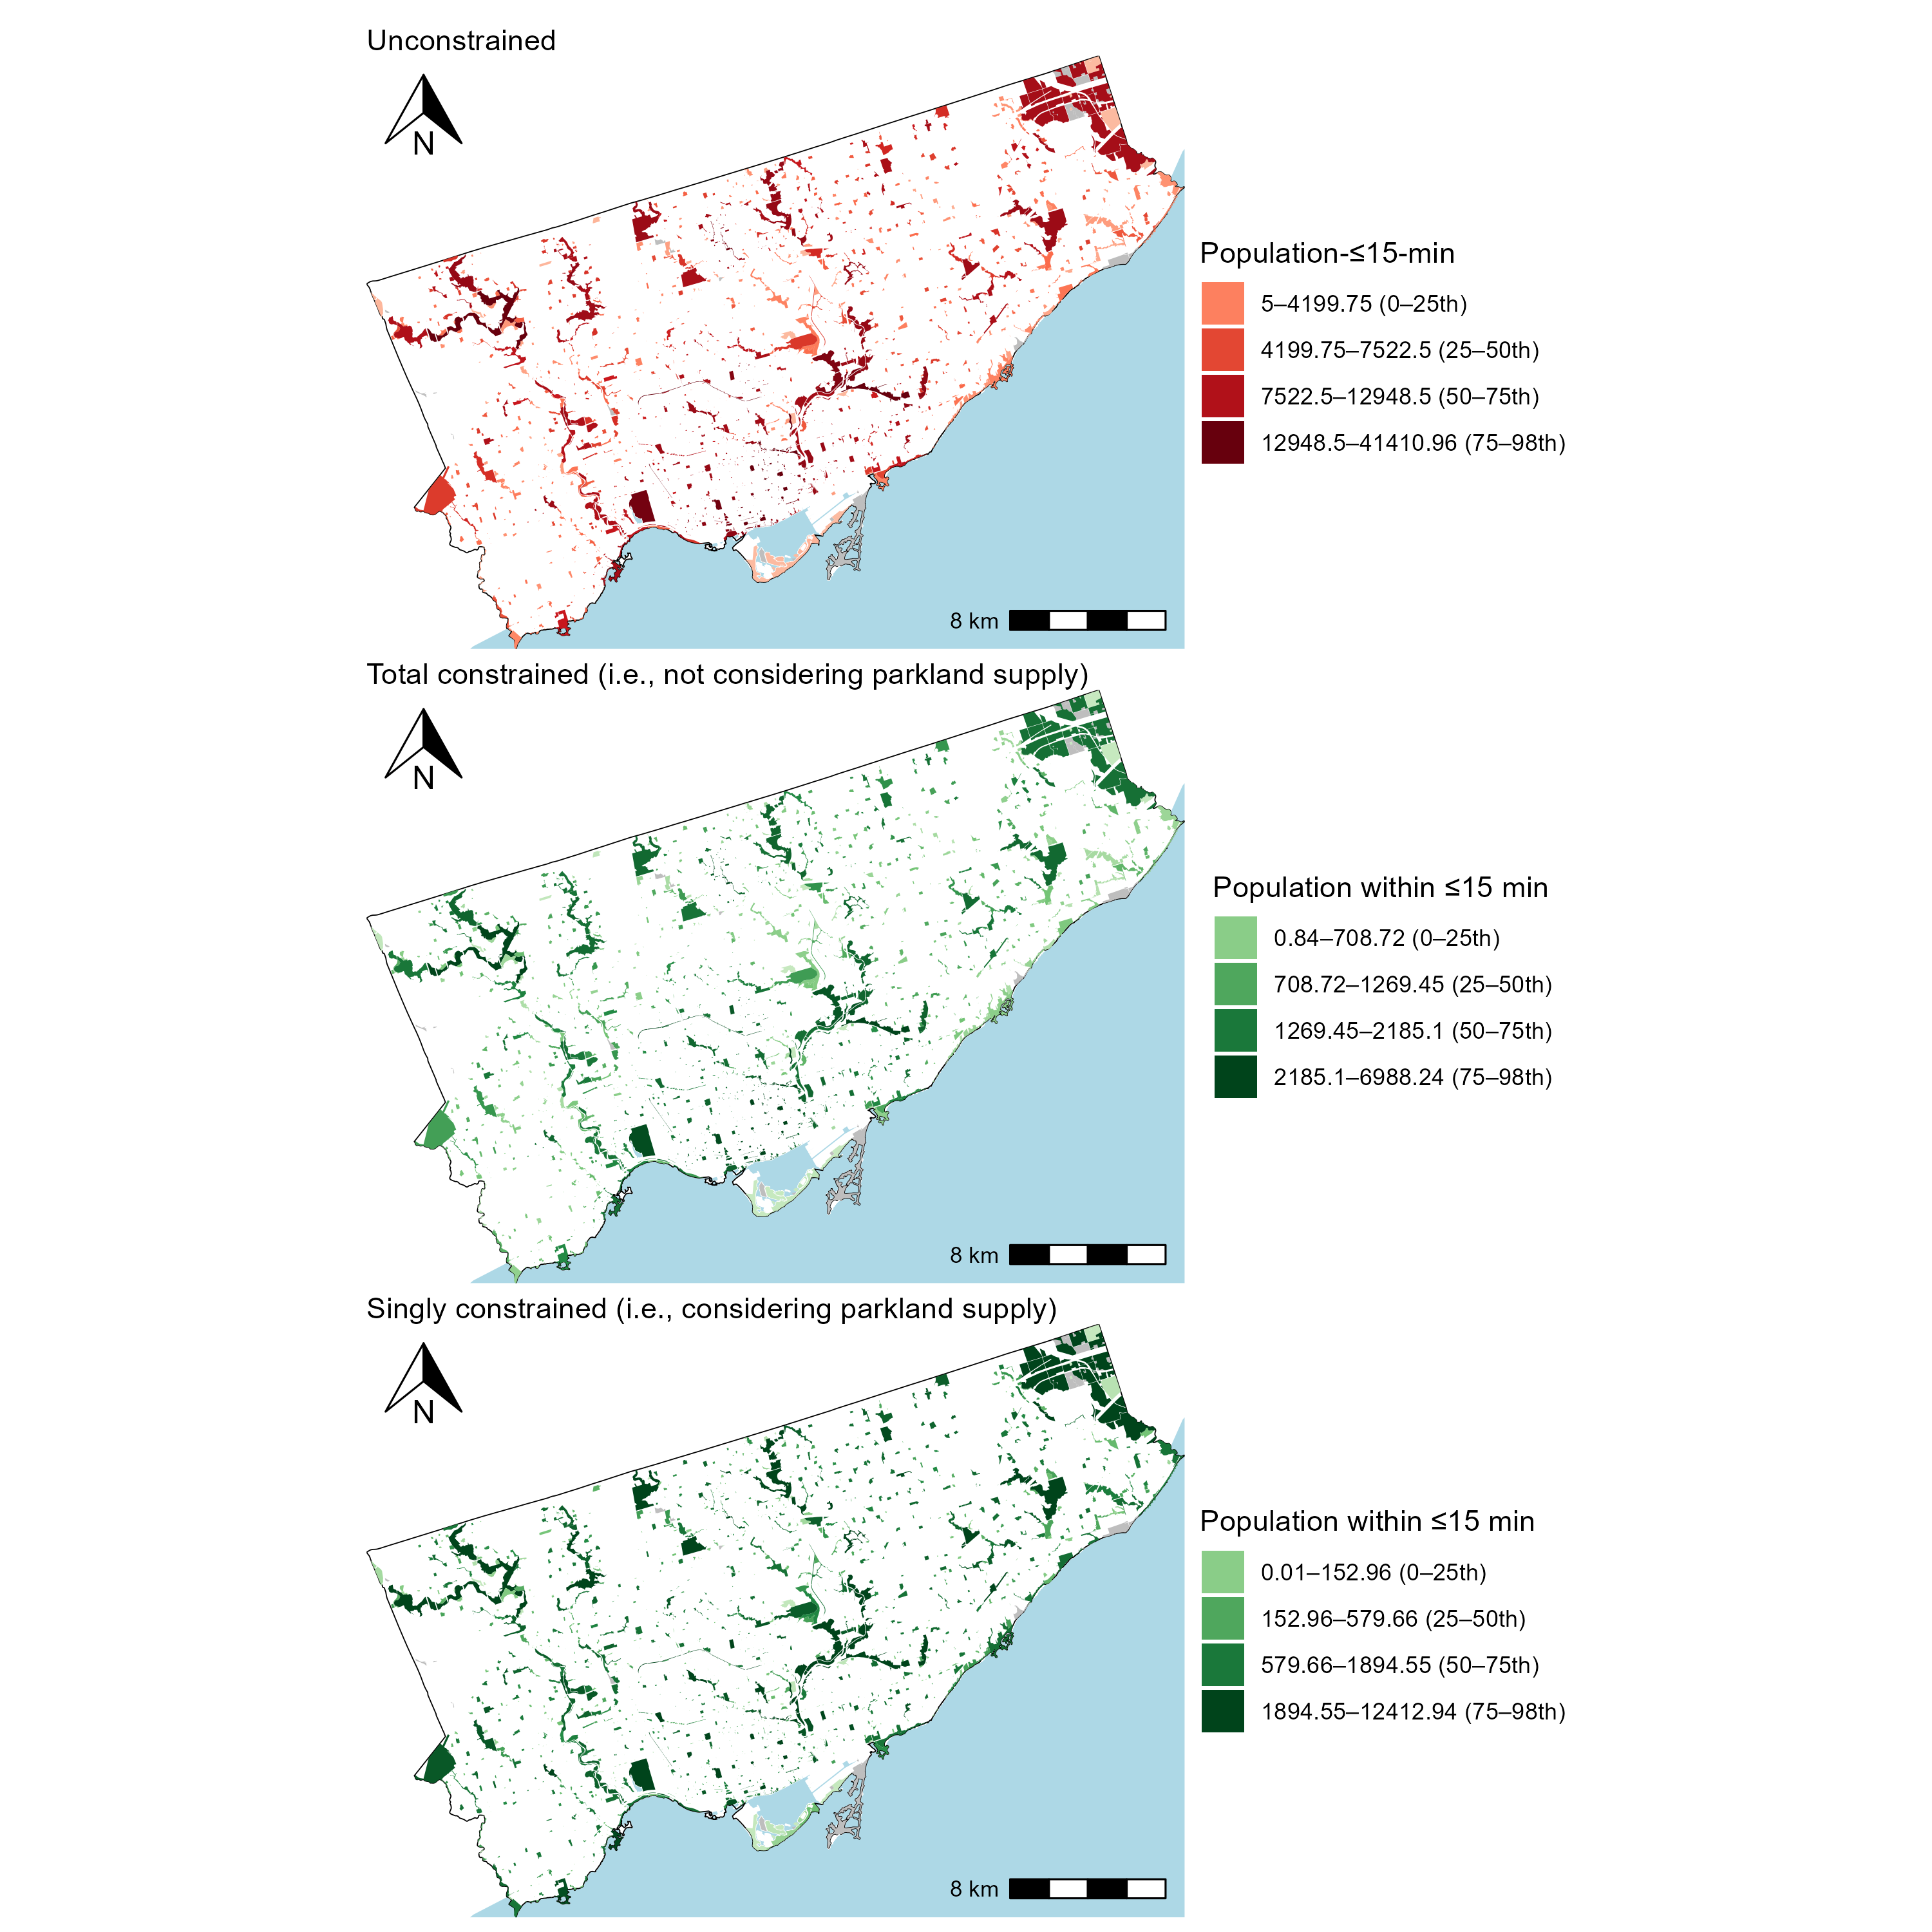
\includegraphics[width=6in]{./data/figures/chp4-pop_access_DB_WALK_plots} 

}

\caption{\label{fig:chp4-pop_access_DB_WALK_plots}Accessibility to population per park in the city of Toronto.}\label{fig:unnamed-chunk-66}
\end{figure}

Figure \ref{fig:chp4-pop_access_DB_WALK_plots} visualises the unconstrained and total constrained measures that are proportional in their magnitude as maintained by the \(\hat K^T\) balancing factor, and the singly and total constrained values are within similar ranges with the singly constrained measure demonstrating a larger range and variance than the total constrained measure. Beyond these commonalities, the constrained values from Figure \ref{fig:chp4-pop_access_DB_WALK_plots} should be interpreted as the accessible population as opposed to the accessible parkland area. As well, each constrained measure sums across the region to equal the total amount of population that we assume can reach parks: 2761103 people.

Unlike the DBs, a spatial unit with less significance for planning (compared to the neighbourhood aggregation at least), the park itself is worth examining. Due to the proportionality, parks per park size classification can be compared by their ratios of \emph{accessible population} to their park size as shown in Figure \ref{fig:chp4-pop_access_byparksize_WALK_plot}. It can be seen that Parkettes and Small Parks serve population at a more efficient parkland area rates than the larger parks using the total constrained measure. Furthermore, when parkland supply is considered (i.e., allocation is based on the area of the park itself and its travel impedance and not only its proximity to population and associated travel impedance), the intensity of the dynamic changes. For instance, smaller parks are still more `efficient' than larger parks but not as much. Small Parks do not `over' allocated, despite their tendancy to be more centrally located. Conversely, larger parks tend to be allocated more to populations, though are relatively less centrally located as the populations face lower competition. Overall, depending on which measure is used: their efficiency of `population service' will differ.

\begin{figure}

{\centering 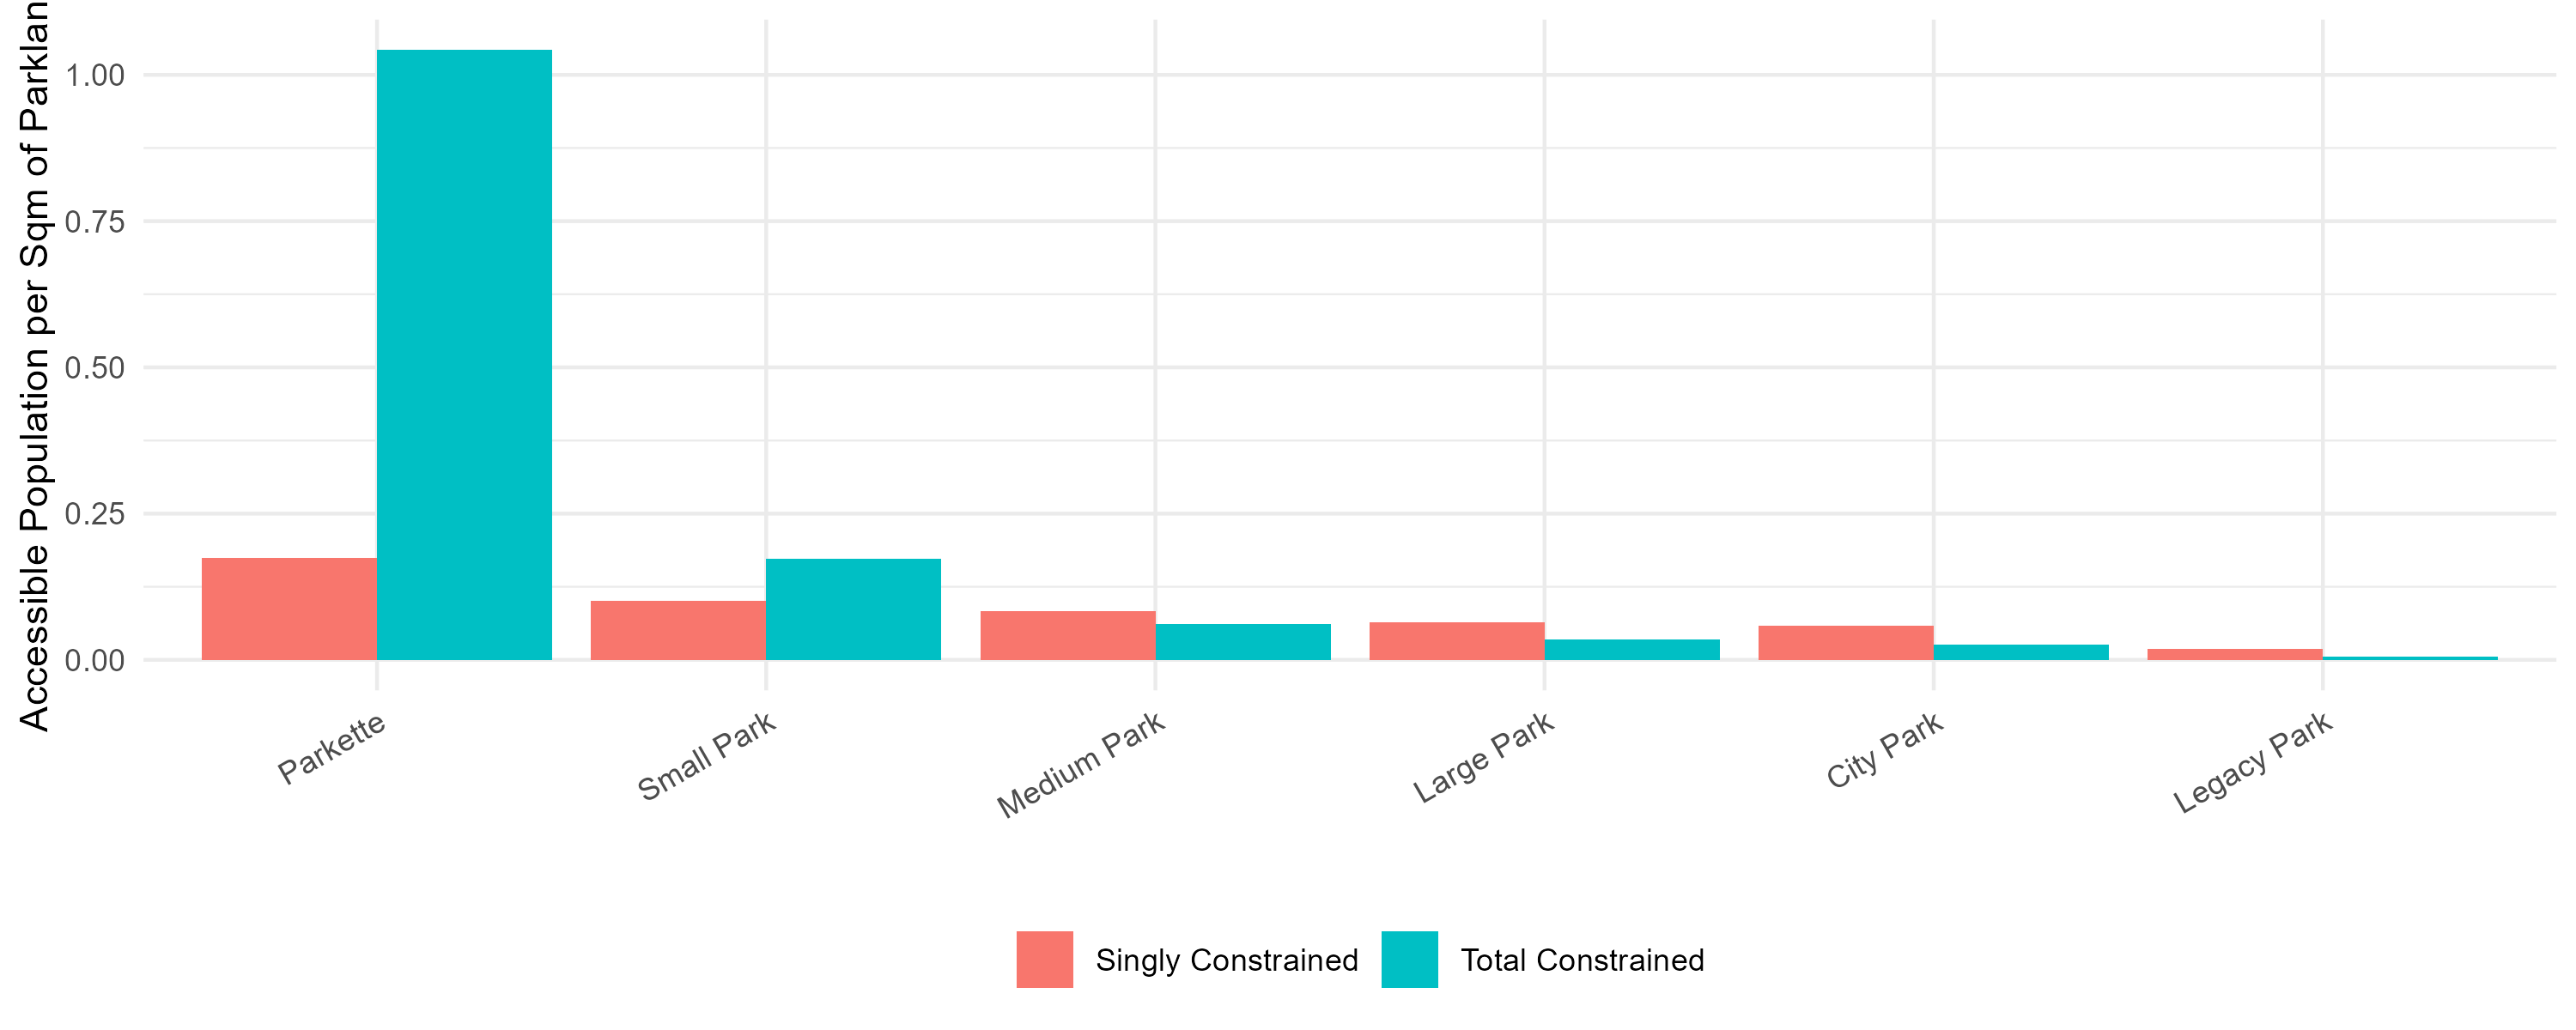
\includegraphics[width=6in]{./data/figures/chp4-pop_access_byparksize_WALK_plot} 

}

\caption{\label{fig:chp4-pop_access_byparksize_WALK_plot}Constrained accessible population per parkland area by park size classification.}\label{fig:unnamed-chunk-67}
\end{figure}

\subsection{Neighbourhood-level accessible population}\label{neighbourhood-level-accessible-population}

Like in the preceding section of the chapter, the neighbourhood can serve as a useful spatial unit for analysis. They align well with both population distribution and parkland organisation in the city. The majority of parks are fully contained within a single neighbourhood, allowing for meaningful calculation of ratios such as accessible population per unit of parkland. Additionally, from an equity perspective, neighbourhood-level analysis enables examination of how different types of parks serve populations across neighbourhoods with varying characteristics, supporting more targeted policy evaluation.

In the Figure \ref{fig:chp4-pop_access_neighbourhood_WALK_plots}, all \(M^0_{ij}\), \(M^T_{ij}\) and \(M^S_{ij}\) values are aggregated at the level of the neighbourhood. They can also be divided by parkland area in that neighbourhood (as determined by summing and splitting, if needed, of parkland area within each neighbourhood) and demonstrated as accessible population per parkland sqm as in Figure \ref{fig:chp4-pop_access_neighbourhood_perparland_WALK_plots}.

\begin{figure}

{\centering 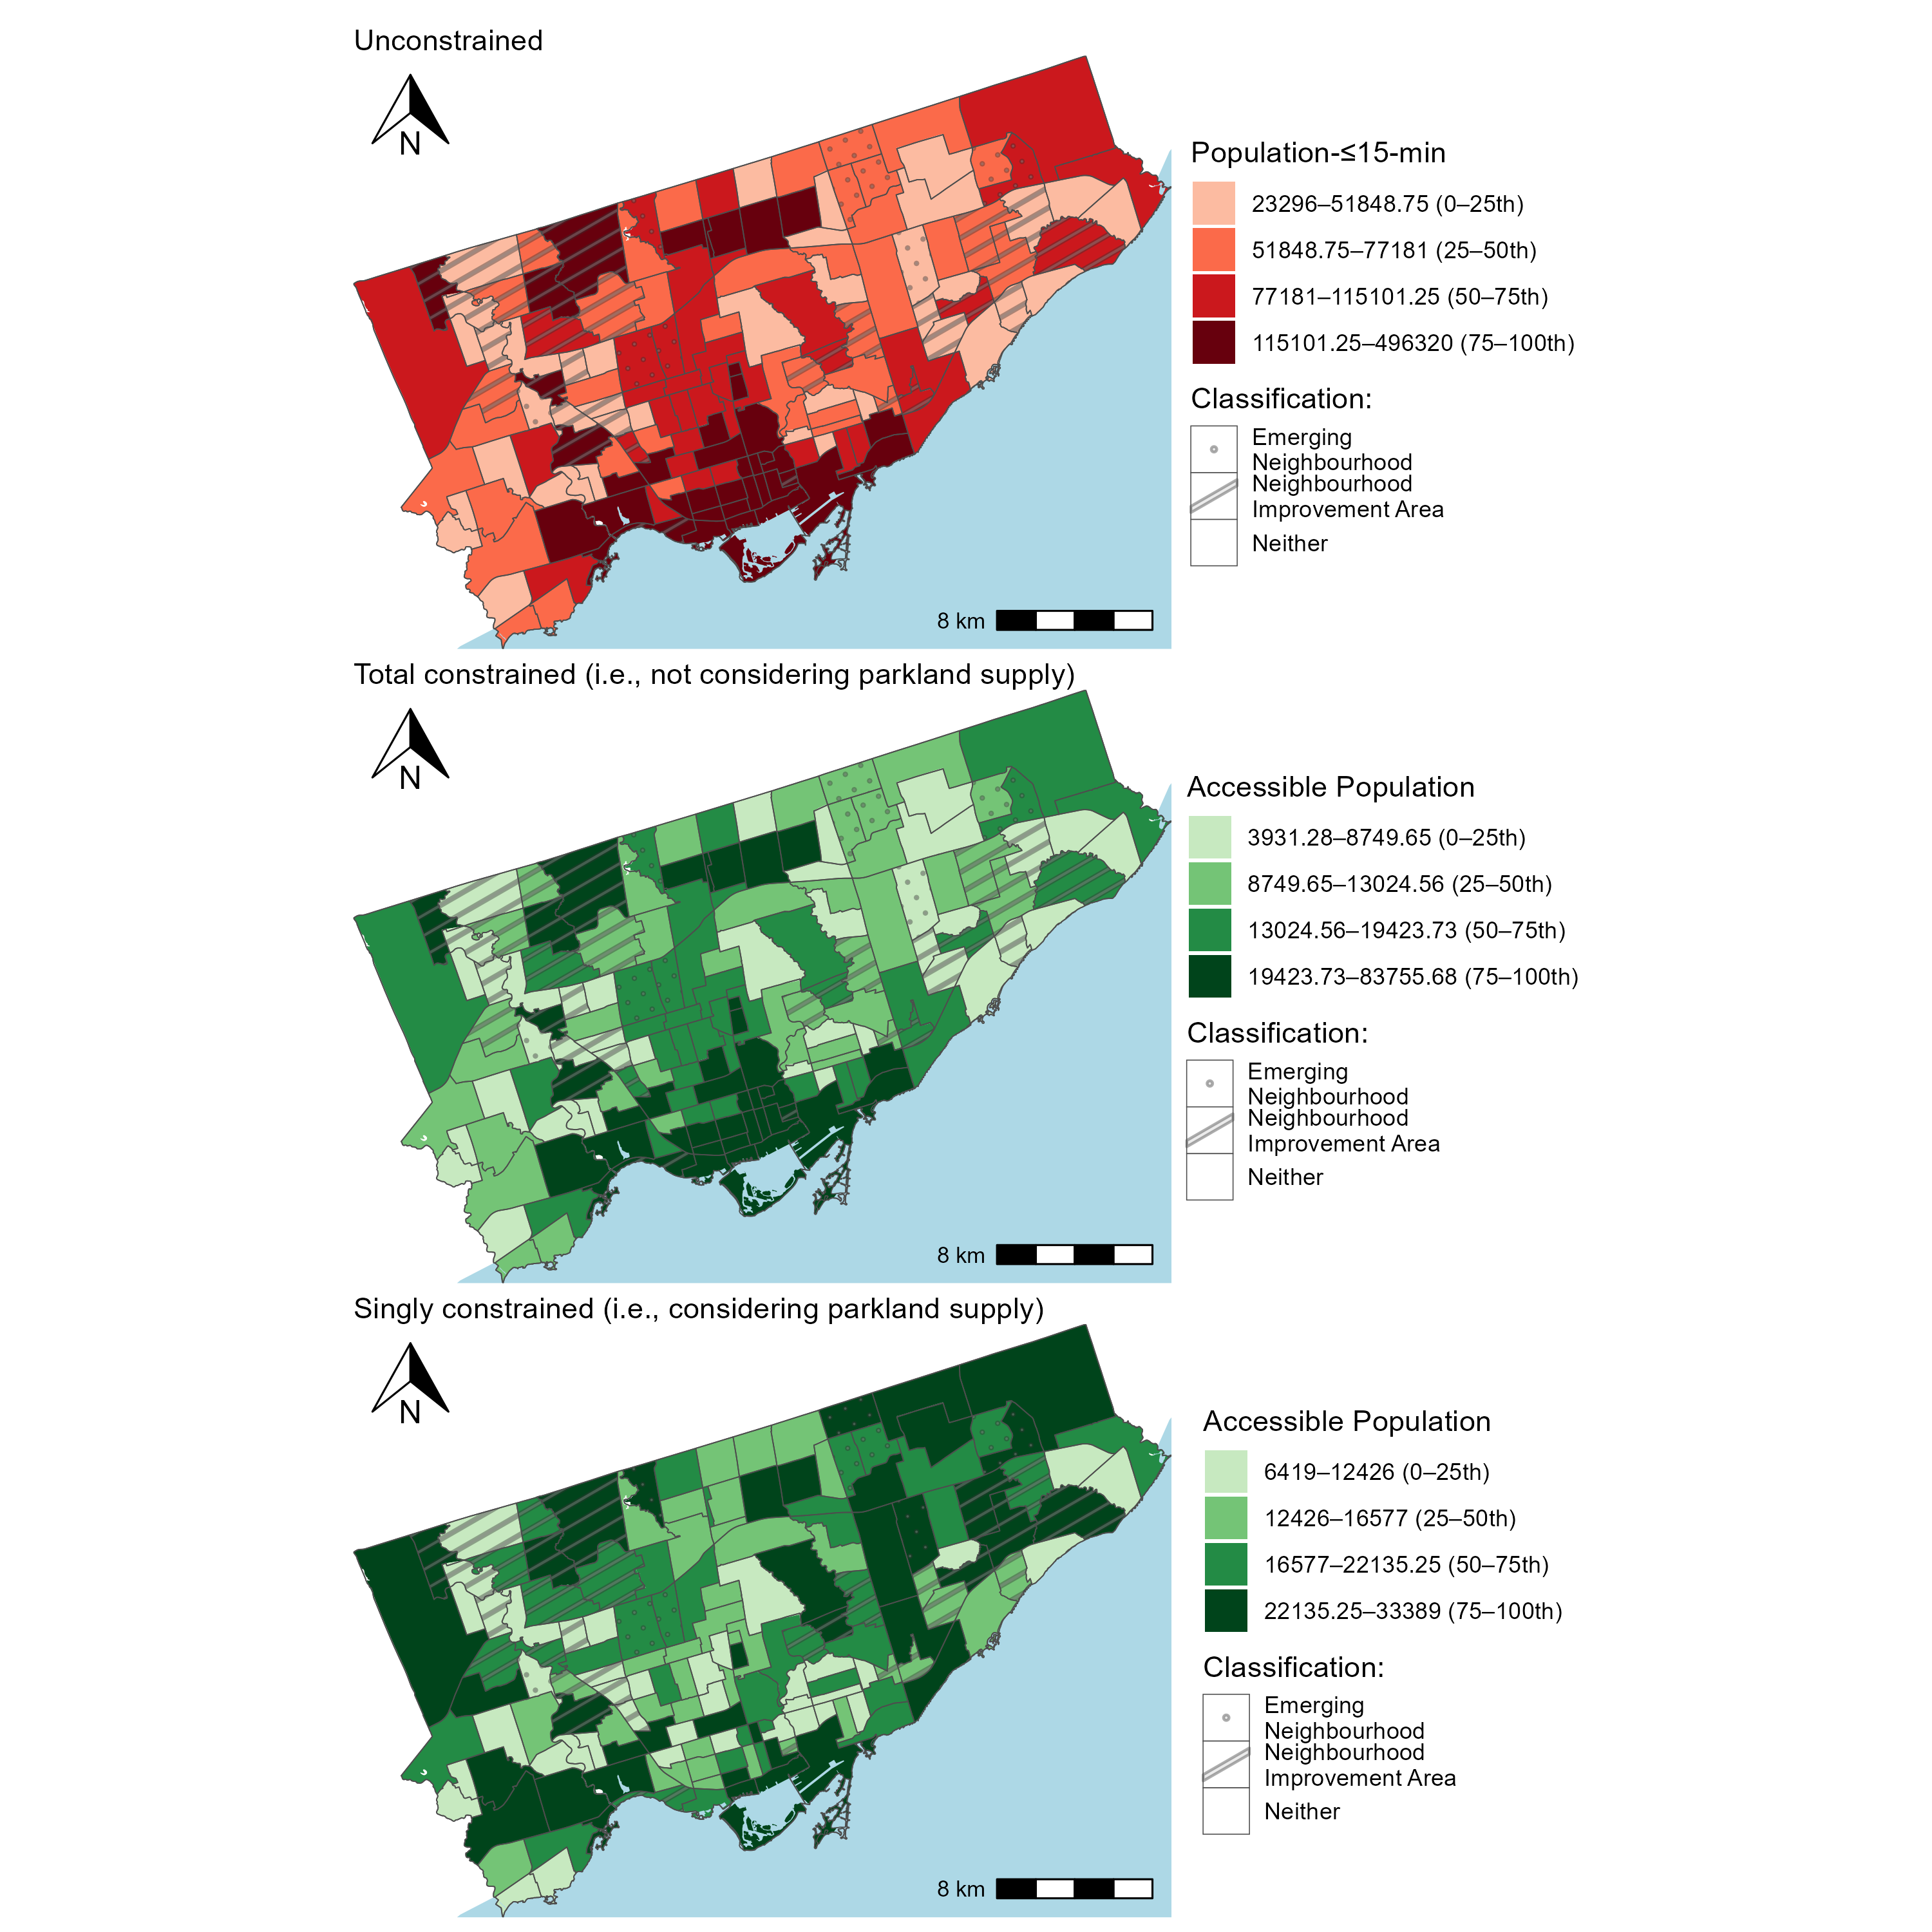
\includegraphics[width=6in]{./data/figures/chp4-pop_access_neighbourhood_WALK_plots} 

}

\caption{\label{fig:chp4-pop_access_neighbourhood_WALK_plots}Accessibility to population per neighbourhood in Toronto.}\label{fig:unnamed-chunk-69}
\end{figure}

\begin{figure}

{\centering 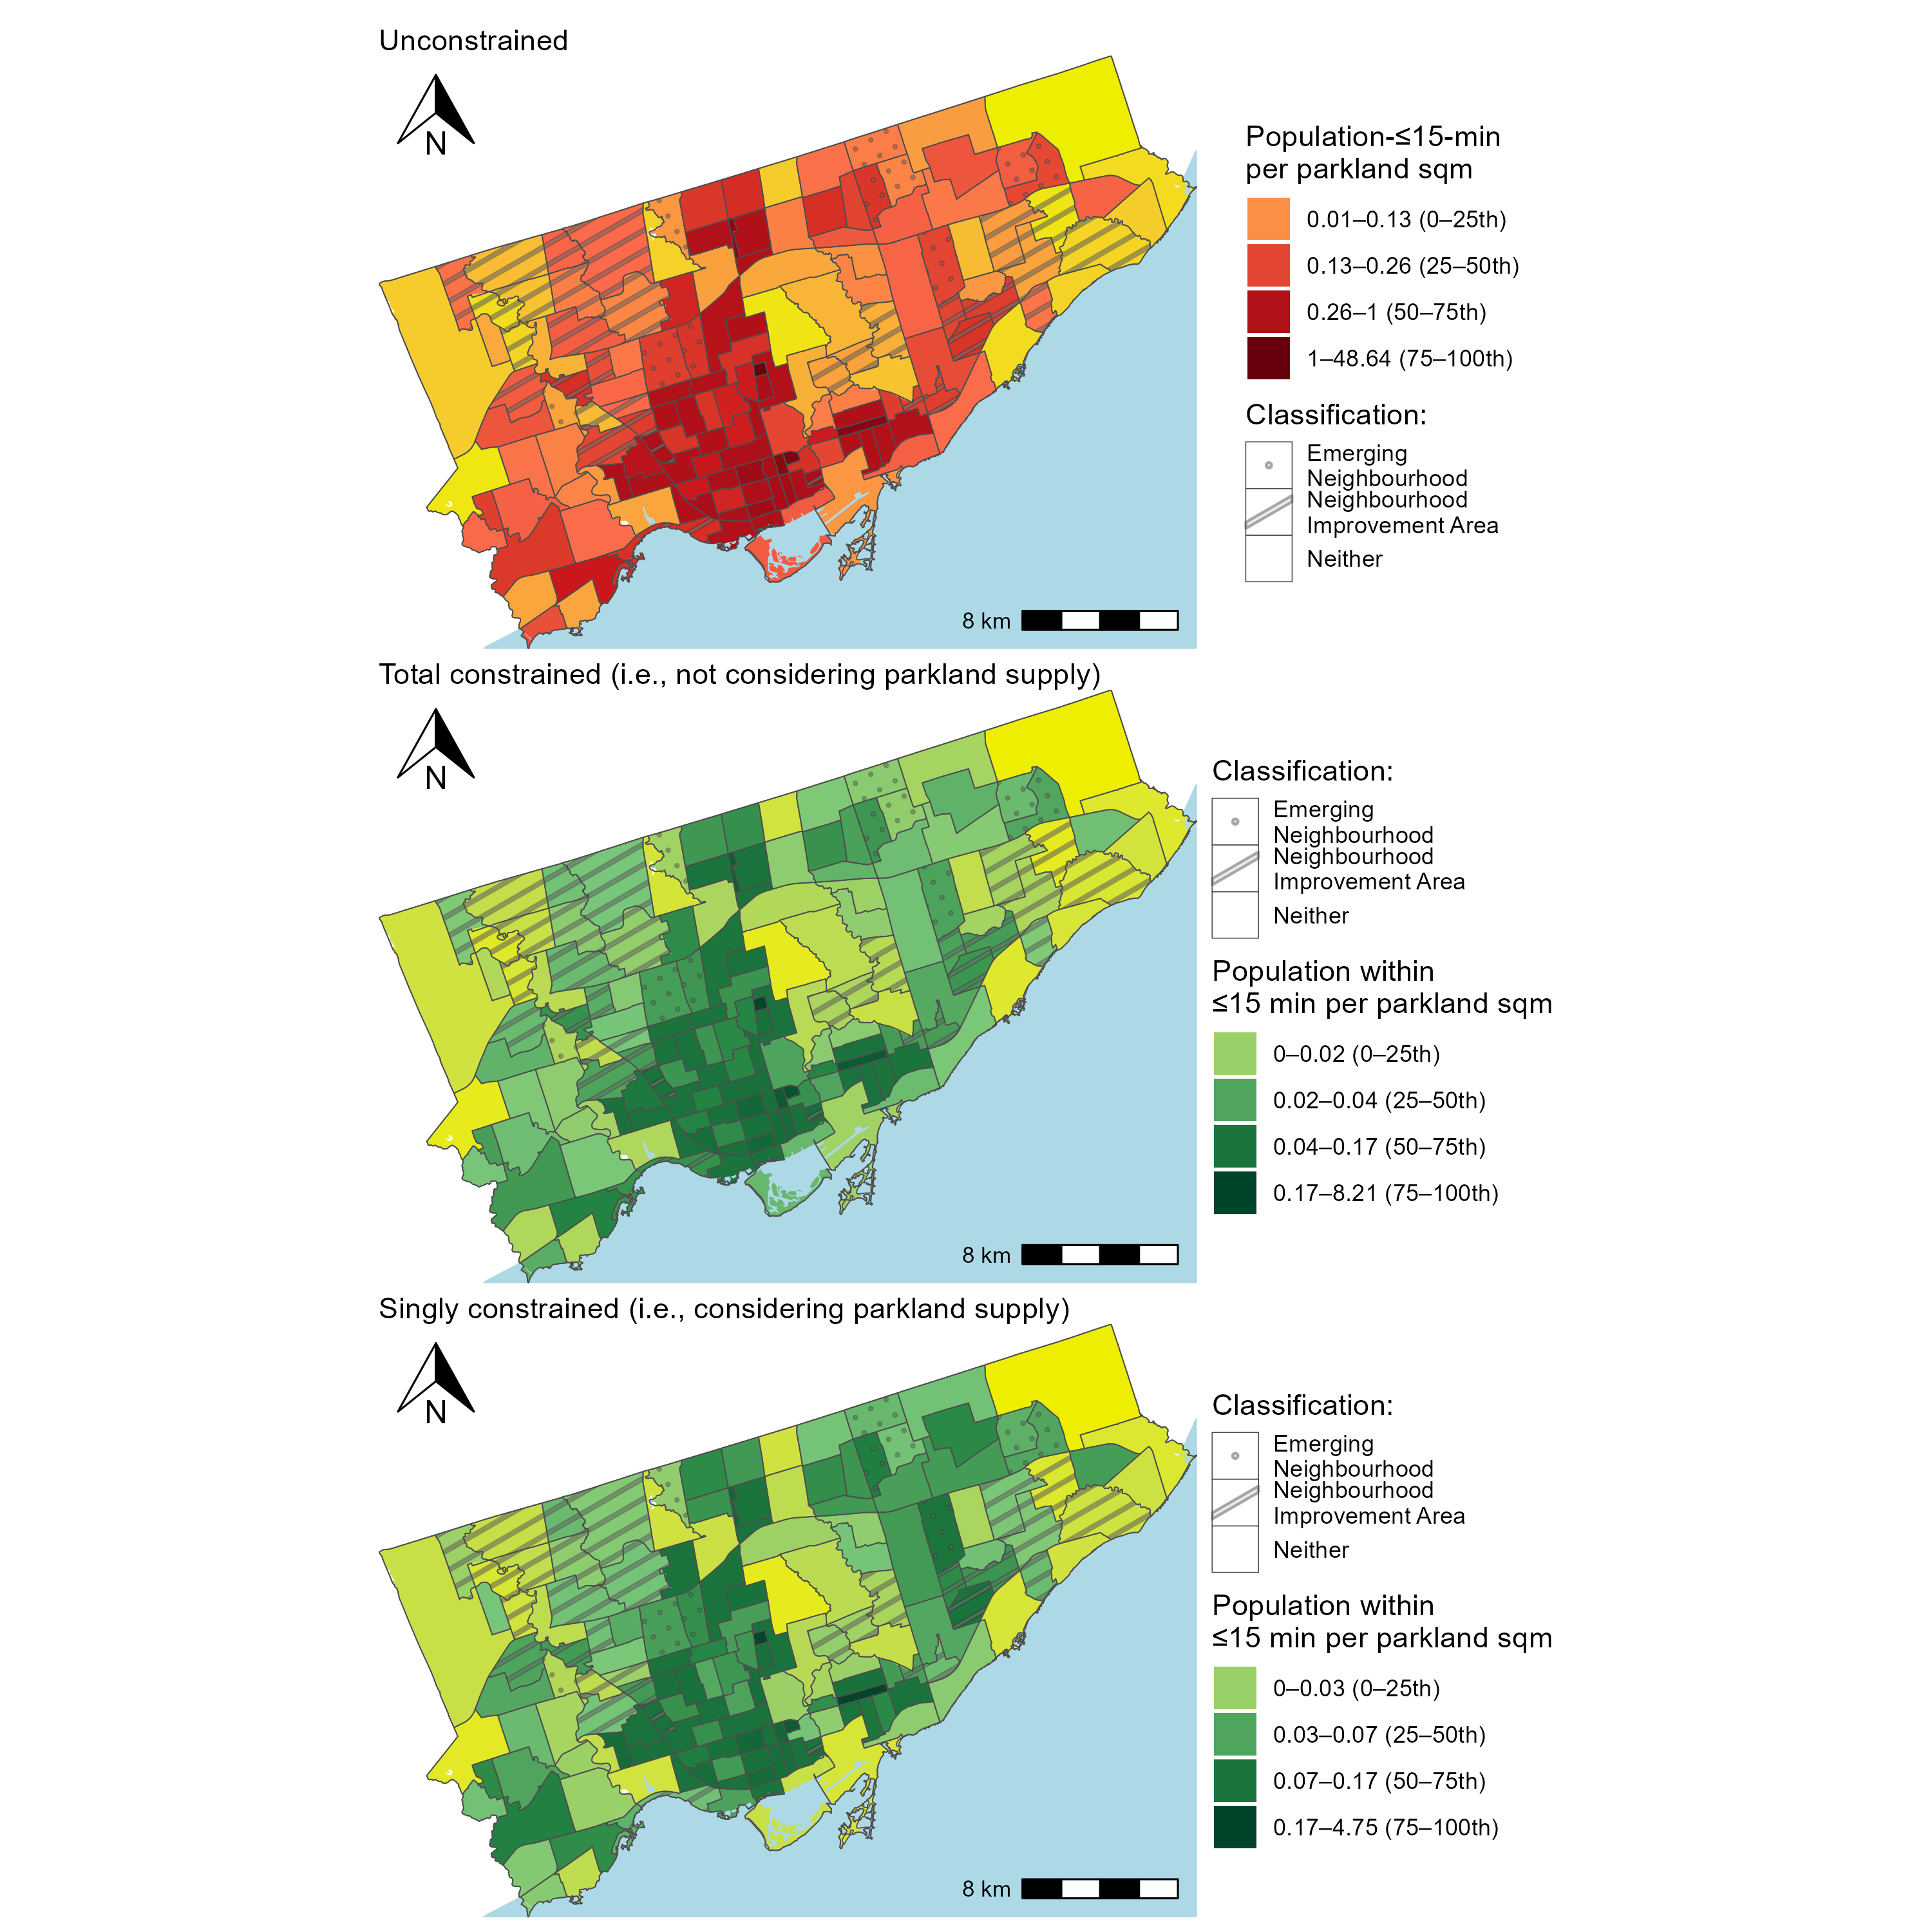
\includegraphics[width=6in]{./data/figures/chp4-pop_access_neighbourhood_perparland_WALK_plots} 

}

\caption{\label{fig:chp4-pop_access_neighbourhood_perparland_WALK_plots} Accessibility to population per parkland sqm at level of the neighbourhood for Toronto.}\label{fig:unnamed-chunk-70}
\end{figure}

Referring to Figure \ref{fig:chp4-pop_access_neighbourhood_WALK_plots} and Figure \ref{fig:chp4-pop_access_neighbourhood_perparland_WALK_plots}, the unconstrained measures are once again shown on their own scale, while the constrained measures are displayed using a shared colour scheme and are within similar ranges. Visually, there is a notable contrast between the total and singly constrained measures: the total constrained map shows higher accessible population values in the downtown core (near the center and shoreline) while the singly constrained map highlights higher values in the northeast and northwest.

The pattern in Figure \ref{fig:chp4-pop_access_neighbourhood_WALK_plots} reflects some intuitive spatial dynamics. The downtown area has a dense population and numerous centrally located parks (especially small ones), resulting in high ``market potential'' under the total constrained measure. However, once parkland supply and population competition are considered (as in the singly constrained measure) these same areas score relatively lower. In contrast, areas in the northeast and northwest, with both substantial parkland and nearby pockets of higher population (and pockets of \emph{no population}), show higher accessibility under the singly constrained measure These neighbourhoods have a more favorable population-to-parkland ratio than the downtown core (i.e., a higher supply of parkland relative to the population in proximity), leading to higher values.

While the raw neighbourhood-level values of the two constrained measures show distinct patterns, normalizing by parkland area (i.e., calculating the accessible population per sqm of parkland) reveals greater similarity between them (Figure \ref{fig:chp4-pop_access_neighbourhood_perparland_WALK_plots}). This is likely because population is typically more spatially clustered than parkland, leading to different distributions of values at the neighbourhood scale. Consequently, neighbourhoods with high or moderate accessible population under both constrained measures may still show more similar normalized values if parkland availability is either very low or very high, thereby producing more comparable ratios between the measures.

Overall, the constrained measure plots in Figure \ref{fig:chp4-pop_access_neighbourhood_perparland_WALK_plots} are interesting as they can be understood to reflect, roughly, how efficiently population is being served by park space in the neighbourhood. This ratio may be useful in flipping the investigation of `where to put new parkland supply' to identifying which neighbourhoods could benefit most efficiently in enhancements to existing parkland area.

Furthermore, non-NIA/ENs and those that are NIA/EN can be investigated. Notably, non-NIA/ENs tend to have \emph{higher} accessible population per sqm of parkland: population more `efficiently' utilises parkland area. Under the total constrained measure, their median is 0.078 people/sqm, and 0.089 people/sqm under the singly constrained measure. In contrast, EN/NIA neighbourhoods show much lower medians (total: 0.038 and 0.029, singly: 0.062 and 0.045). This finding mirrors the per capita neighbourhood \emph{accessible parkland} analysis findings. However, the choice of aggregation unit and denominator will strongly influences results, and analysts must be attentive to these decisions when interpreting accessibility metrics.

\subsection{Summary}\label{summary-1}

Ultimately, examining population-constrained accessibility from the park itself \emph{and} from the neighbourhood provides valuable insight for planning of parkland service through the perspective of population potentially served. It allows analysts to:
- Understand how many people are served by each park, both in total and per parkland (or summed and normalized by some other zonal unit variable);
- Identify over- or under-performing parks. For example, parks near large populations but lacking amenities may represent strategic opportunities for investment to improve service efficiency.

In sum, analyzing the \emph{accessible population} approach can serve as a complimentary way in analyzing parkland service provision, among other questions that relate to how accessible the population is to opportunities.

\section{Conclusion}\label{conclusion}

This chapter presents the calculated accessibility scores across the following dimensions:

\begin{enumerate}
\def\labelenumi{\arabic{enumi}.}
\tightlist
\item
  Unimodal total constrained \textbf{accessible parkland} summarised per origin zone \(V_i^T\) (i.e., DB) and then per neighbourhood. All people (in DBs) to all parkland area (in parks) by a 15-minute walk is assessed. This measure can be interpreted as ``how much parkland area is potentially reachable by the walking-population from this zone?''. The measure is also presented as a `parkland provision' ratio of parkland per walking-population.
\item
  Unimodal total constrained \textbf{accessible population} summarised per destination zone \(M_j^T\) (i.e., the park itself) and then per neighbourhood. This measure is the \(ij\) transpose of \(V_i^T\), and can be interpreted as ``how much walking-population is potentially reachable from this park?''. The measure is also presented as a potential population `service catchment' or a ratio of population potential per parkland area at the park level and at the neighbourhood level.
\item
  Both of the above constrained accessibility measures are compared to the conventional calculation of accessibility, or what is referred to in this work as unimodal unconstrained \textbf{accessible parkland} summarised per each DB \(V_i^0\) and \textbf{accessible population} summarised per park \(M_j^0\). These measures assess the same walking network but do not consider any zonal or regional constraints. As such, these conventional measures only offer insight into the proportion of potential reachability. Unlike the constrained measures, no provision or catchment ratio can be meaningfully calculated for these measures.
\end{enumerate}

Overall, constrained accessibility provides a more interpretable and policy-relevant framework than unconstrained methods. These measures allow analysts to:

\begin{itemize}
\tightlist
\item
  Identify DBs with poor access to parkland. This could be DBs in equity-seeking neighbourhoods (NIA), helpful in highlighting areas that may warrant new parks or improved access.
\item
  Identify parks with low population reach, revealing underutilized assets or areas where connectivity enhancements could expand service reach. This can be seen as a transpose understanding of the first point, but with its interpretation meant for a different communication.
\end{itemize}

However, the analysis in this chapter only considered accessibility by one mode: walking. A key consideration is missing: parks can be reached not only by walking, but by other more far-reaching modes. People travel by transit, cycling, and driving--each with their own distinct behavioural patterns (as discussed in Chapter 3). Unconstrained accessibility measures do not have consistent methodologies for considering multiple modes, but as introduced, the constrained measures can be extended to consider multimodal analysis. Hence, in the following chapter, the multimodal extension of the constrained measures will be detailed and compared, when possible, to the unconstrained case.

\chapter{Multimodal accessibility to parks in Toronto}\label{multimodal-accessibility-to-parks-in-toronto}

\section{Overview}\label{overview-4}

This chapter details \emph{multimodal} accessibility of parkland from the perspective of parkland area and population. Like the unimodal example, origin and destinations are DB and park entrance points, and their masses are modal population per DB \emph{or} mode-specific parkland area (in hectares) per park. The normative impedance functions for all modes discussed in Chapter 3 are adopted.

In the first half of the chapter, the focus is on \emph{multimodal accessible parkland area}. The variables of \(V^{m0}_i\), \(V^{mT}_i\) and \(V^{mS}_i\) represent the mode-specific quantities of multimodal accessible parkland area for each DB. The sum of these variables are first detailed which provides an aggregate measure of multimodal accessible parkland area per DB, then the mode-specific values are plotted and discussed. Following this, the accessible parkland per capita ratio is demonstrated and a discussion on multimodal `potential parkland service provision' is detailed.

In the more brief second half of the chapter, the focus is on \emph{multimodal accessible population} and the variables of \(M^{m0}_j\), \(M^{mT}_j\) and \(M^{mS}_j\) represent the mode-specific quantities of multimodal accessible population for each park. The mode-specific values are plotted per park and discussed.

This chapter is concluded by a comparison and discussion of the aggregated multimodal accessible parkland area and multimodal accessible population values for the 6 former municipal boundaries. These values are compared to their tangible counterparts: the amount of population residing in each former municipality (for accessible multimodal parkland area) and the number of actual parkland area in each former municipality (for accessible multimodal population), effectively: ratios of multimodal parkland area potentially provided and ratios of multimodal population potentially served.

\section{Multimodal accessible parkland (for the population)}\label{multimodal-accessible-parkland-for-the-population}

First turning to the concept of \emph{multimodal accessible parkland}, the results in this section include those calculated by unconstrained and constrained multimodal measure. Each measure yields different results (i.e., the amount of parkland area that is accessible by a certain mode at a specific zone) depending on the assumptions contained within the accessibility calculation. For the unconstrained measure, the values proportionally reflect the amount of accessible parkland area by mode: as there is no proportionality constant to maintain the resulting values units. For the constrained measures, the values remain a proportion of the regional total and/or the parkland area of each specific park allocated to each origin. Each origin can also be defined by the amount of mode-share present; the use of mode-share as an origin weight is only relevant for the singly constrained accessibility measure, and differences between results will be discussed.

Beginning with unconstrained accessibility, Figure \ref{fig:chp5-mm_parkland_unconc_access_DB_plots} displays the unconstrained accessibility to parkland area, calculated for each mode separately. The scale is in deciles. DBs with no accessibility are shown in medium grey and DBs with no population are shown in light grey. These lighter grey areas are typically commercial or industrial in land-use, and were dropped before calculating any accessibility measure to better reflect the motivation of this analysis: spatially accessible parkland area from a location \emph{for} the population. Furthermore, travel impedance functions (and associated travel times) are different depending on the mode. To aid in comparability, multimodal values are placed on the same scale across all four plots, but their units are different depending on the mode. For cycling and walking, it can be understood as accessible parkland-ha-within-15-minutes, whereas for transit and car it is parkland-ha-\(e^{-0.02}\) and parkland-ha-\(e^{-0.04}\).

\begin{figure}

{\centering 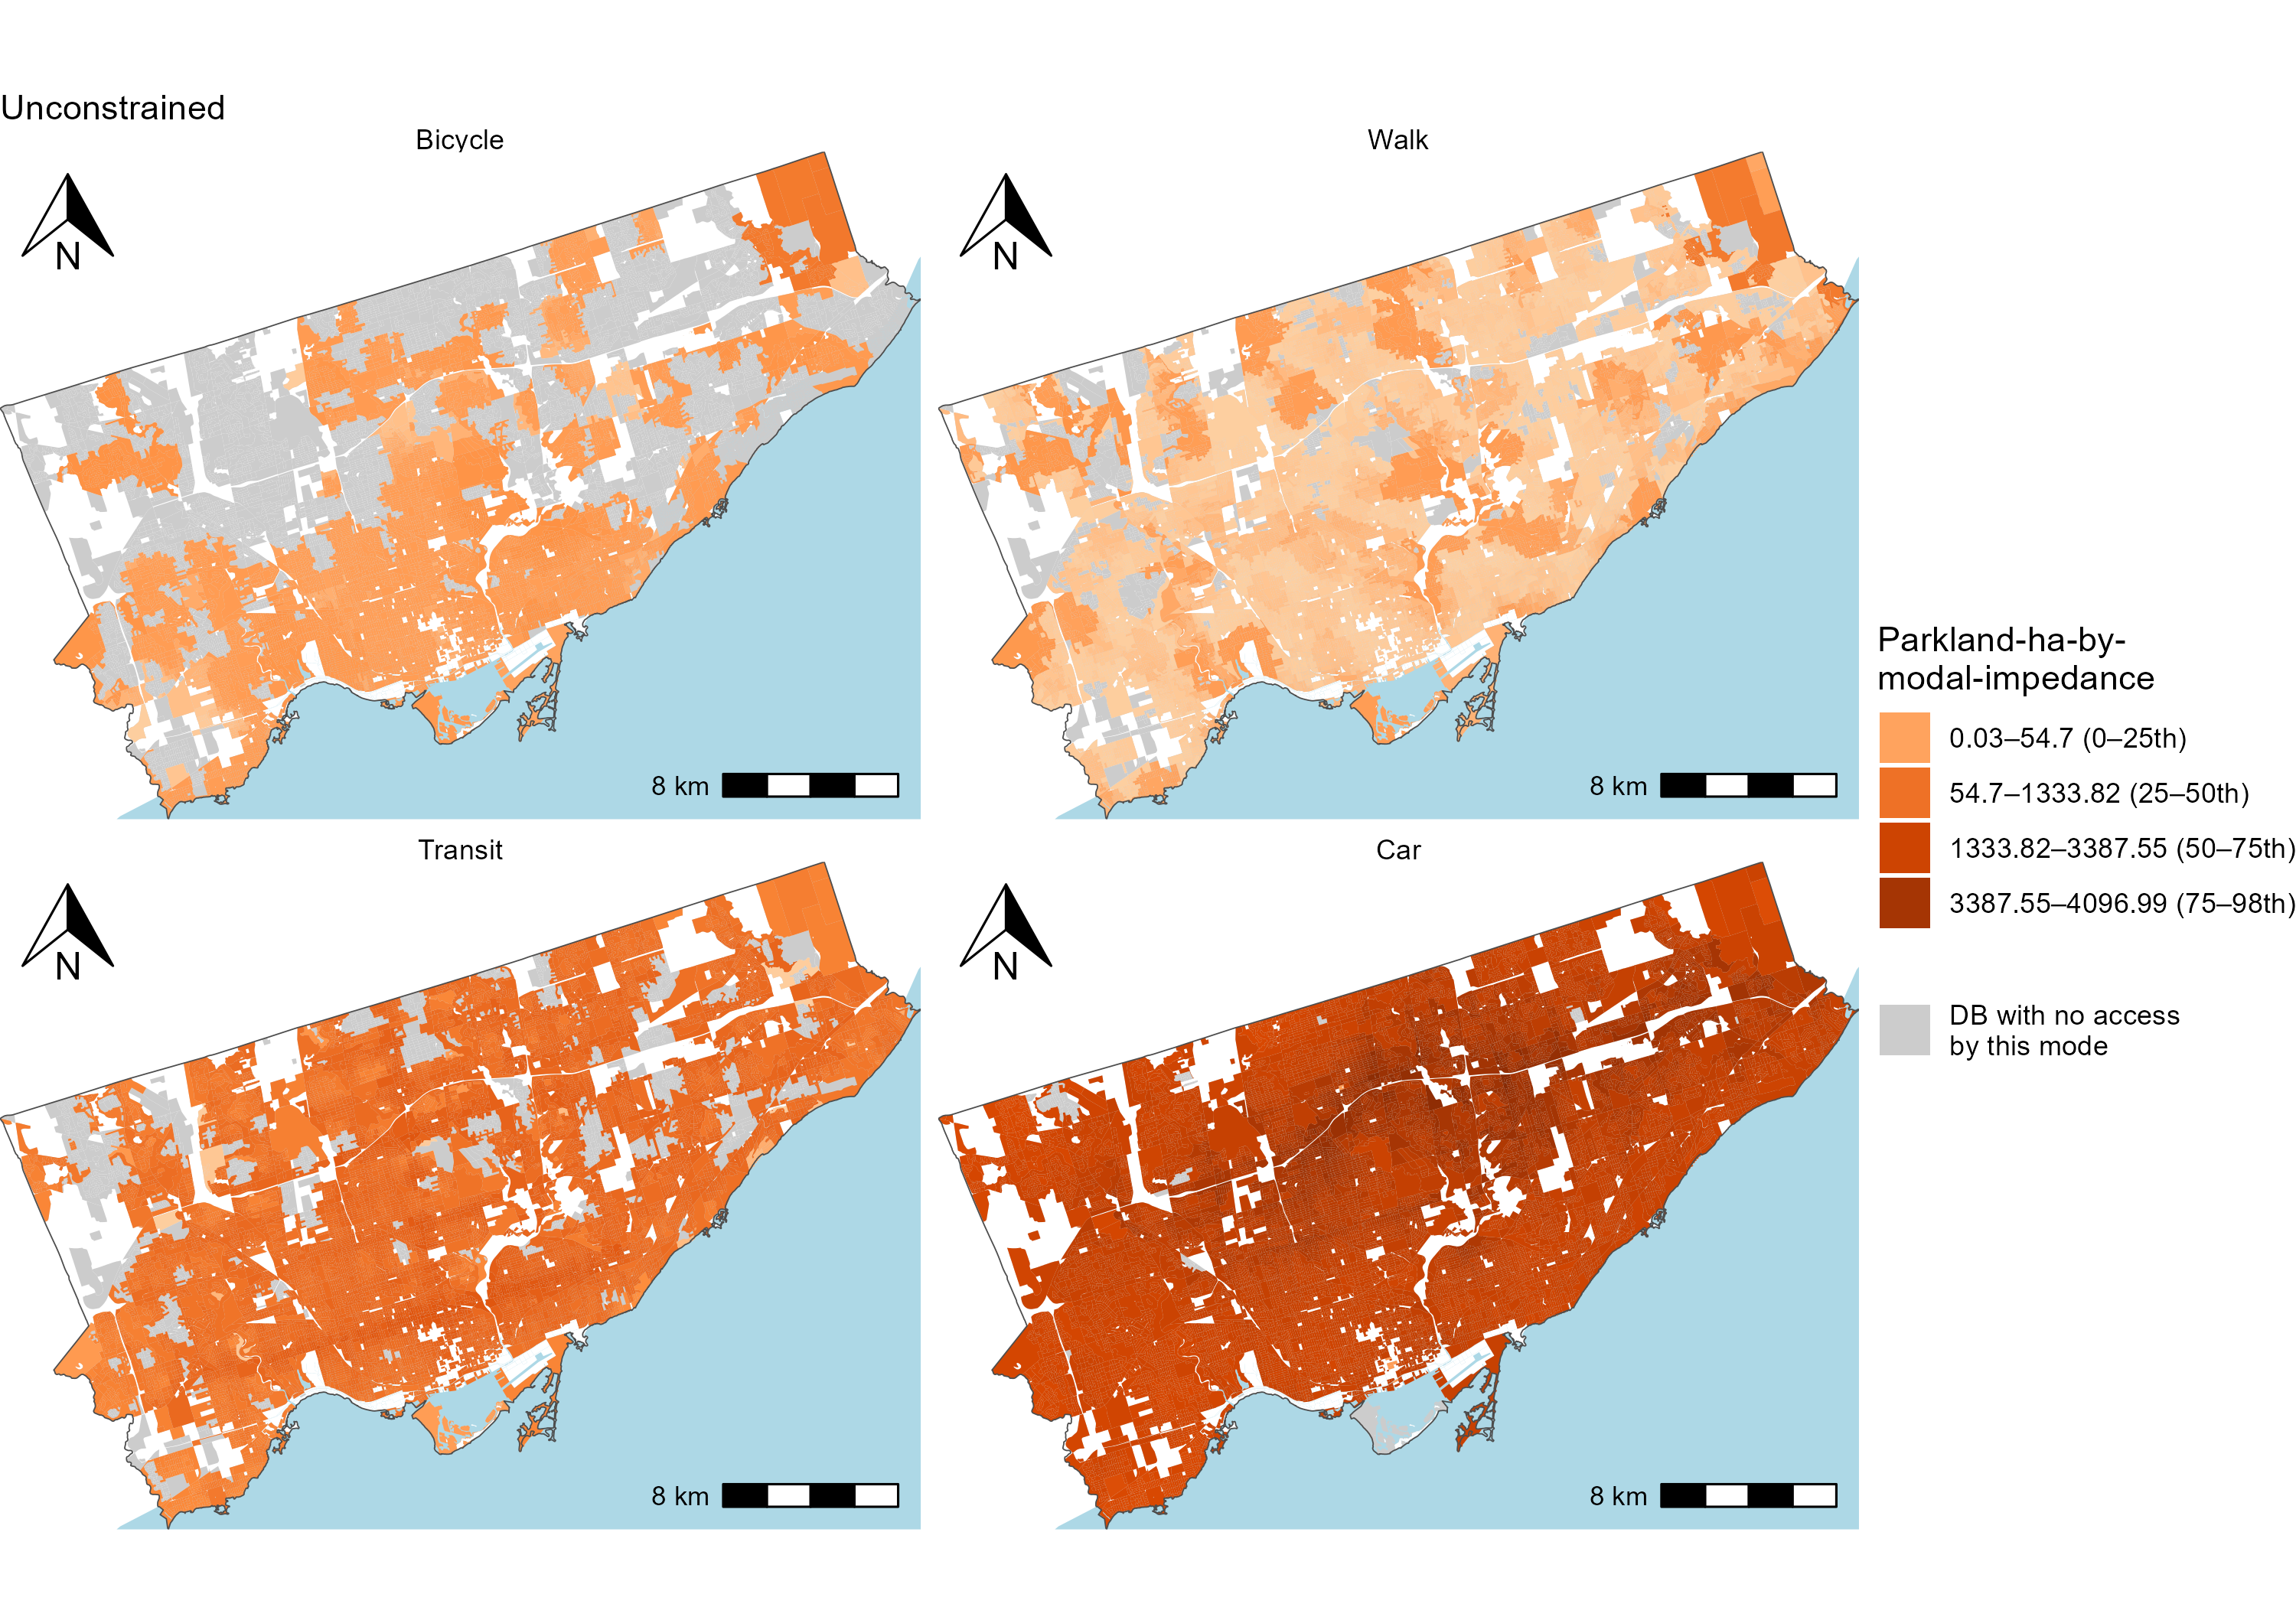
\includegraphics[width=6in]{./data/figures/chp5-mm_parkland_unconc_access_DB_plots} 

}

\caption{\label{fig:chp5-mm_parkland_unconc_access_DB_plots}Accessibility to parkland area per DB as measured by the unconstrained accessibility measure for multiple modes.}\label{fig:unnamed-chunk-74}
\end{figure}

In Figure \ref{fig:chp5-mm_parkland_unconc_access_DB_plots}, for non-motorized modes it can be observed that many pockets of the city offers lower levels of accessibility by walking and slightly higher levels by cycling. Highest levels of accessibility are in close proximity to parks. For motorized modes, transit offers moderate levels of accessibility, with highest levels near the subway routes as well as routes (not pictured) with higher frequency transit opperation (i.e., higher frequency buses and streetcars). Lower levels of transit accessibility are reflected of where there are lower amounts of parks and transit service. For car mode, accessibility is highest along the east-west expressway north in the city: where car speeds are high and a large amount of parkland area is accessible. Recall: motorized travelers can travel up to 120 minutes, though with diminishing likelihood is assumed as the travel time increased, and motorists do not access smaller parks. Conversely, non-motorized travelers are capped to a maximum 15 minutes of possible travel time.

Another key observation about Figure \ref{fig:chp5-mm_parkland_unconc_access_DB_plots} is that it does not represent truly multimodal accessibility. Each plot evaluates parkland accessibility for a single mode in isolation, without accounting for interactions with other modes. However, the scores could still be compared across modes (as done in the previous paragraph) since they share a common intuitive measurement scale `parkland-ha-by-modal-impedance'--though meaning cannot be gleaned from the values themselves as the underlying units are not identical across modes.

This issue of inconsistent units is remedied using the multimodal constrained accessibilty measures. Figure \ref{fig:chp5-mm_parkland_conc_access_DB_plots_summedmodes} demonstrates the total constrained and singly constrained DB values aggregated at the level of the DB. The values of each DB consist of a share of the mode-specific multimodal accessible parkland area, which can be summed to reflect the multimodal accessible parkland area of a DB as a proportion of the total parkland area in the region that can be reached from DBs with a population (i.e., 8018.54 hectres). This form of overall multimodal accessible parkland area amount cannot be intuitively calculated using the unconstrained multimodal accessibility measure.

\begin{figure}

{\centering 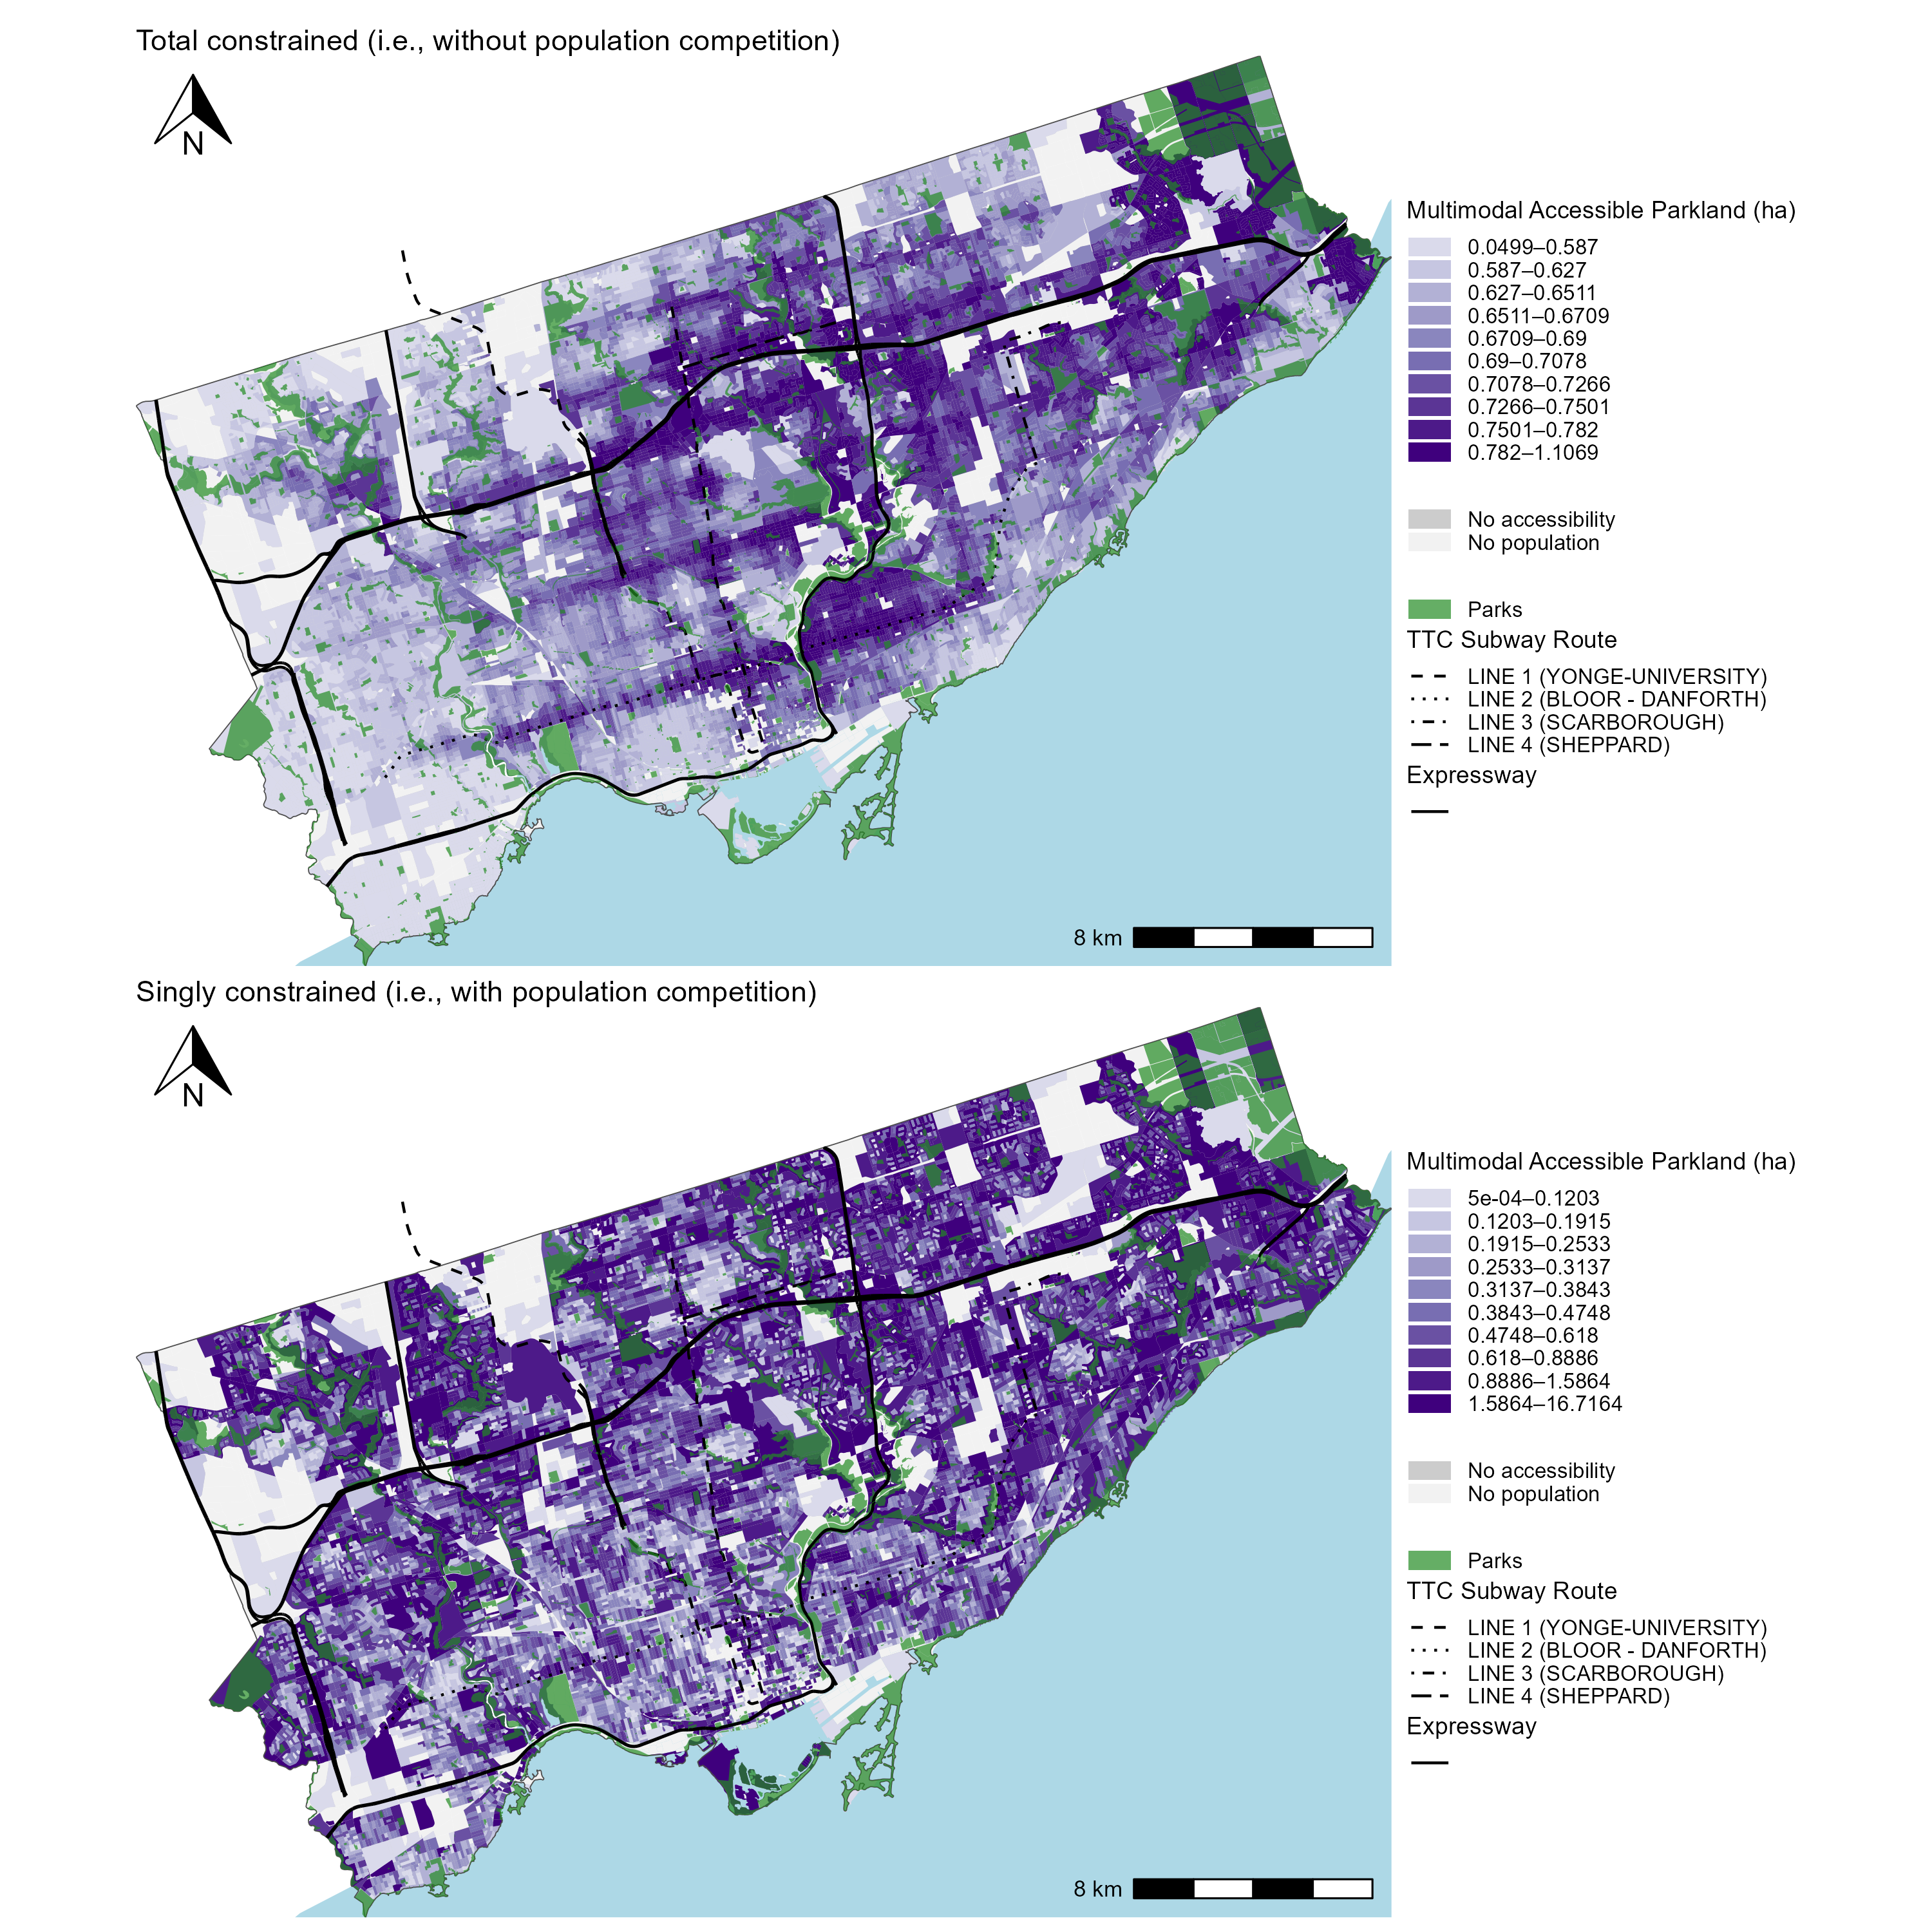
\includegraphics[width=6in]{./data/figures/chp5-mm_parkland_conc_access_DB_plots_summedmodes} 

}

\caption{\label{fig:chp5-mm_parkland_conc_access_DB_plots_summedmodes}Overall multimodal accessibility to parkland area per DB.}\label{fig:unnamed-chunk-75}
\end{figure}

Both constrained measures in Figure \ref{fig:chp5-mm_parkland_conc_access_DB_plots_summedmodes} consider the mode-specific multimodal accessibility in the region under the same framework. For instance, regarding the total constrained plot, the total parkland area in the region is proportionally allocated to the potential mode-using group at each origin defined only by that mode-using group's associated travel impedance value. Recall, the total constrained measure does not use the modal-shares at each origin, allocation is only based on the relative modal travel impedance and mass of the parkland area.

In the total constrained plot in Figure \ref{fig:chp5-mm_parkland_conc_access_DB_plots_summedmodes}, it can be observed that areas of high multimodal accessibility are in areas where where accessibility by both motorized modes is high: i.e., along subways lines which provide high levels of access by transit but also car accessibility by car as they are under relative higher speed streets. It's notable that areas where car accessibility north in the city along the expressway also provide high multimodal accessibility: though that is because car accessibility is exceptionally high, while all other modes are low (as will be later discussed).

On the other hand, the singly constrained map in Figure \ref{fig:chp5-mm_parkland_conc_access_DB_plots_summedmodes} presents a different story. This measure accounts for mode-specific population demand, as determined by the modal share of leisure trips made by the DB population. Unlike the total constrained multimodal values, which tends to be more spatially uniform, both the population distribution and the modal split vary significantly across the city. As a result, the singly constrained multimodal accessibility surface is more uneven. It reflects not only the spatial distribution of population but also the differentiated demand and travel impedance associated with each transportation mode. Overall, this plot reveals higher multimodal parkland accessibility in the northern parts of the city compared to the downtown core, particularly around the central near the `U' of Subway Line 1. This suggests that although the downtown area has a relatively dense parkland network (as seen in the constrained plot), its high population density and greater reliance on shorter-range modes (e.g., walking, cycling, and transit) reduce the relative accessibility of parkland for all.

To explore the differences between modes, the constrained accessibility plots in Figure \ref{fig:chp5-mm_parkland_conc_access_DB_plots_summedmodes} can be decomposed by mode, allowing for an assessment of how much \emph{more} or \emph{less} multimodally accessible parkland is available to each potential mode-using population group. These differences arise in part from the way accessibility is shared or limited by the presence of other groups competing for the same parkland supply. A discussion of this mode-specific analysis is presented in the following subsections.

\subsection{Mode-specific total constrained multimodal accessibility}\label{mode-specific-total-constrained-multimodal-accessibility}

Figure \ref{fig:chp5-mm_parkland_concs_access_DB_plots} displays the mode-specific decomposition of total constrained multimodal accessibility to parkland area (in hectares) at the DB level. All values are displayed on a consistent scale and coloured by decile. Importantly, while these values are proportional to the unconstrained measures, they differ by being expressed in explicit, interpretable units: hectares of multimodally accessible parkland. Travel impedance across modes is made comparable through the use of a common balancing factor, \(K^{mT}\), which balances each mode's unconstrained accessibility flows such that they remain a proportion of the total parkland area in the region. Specifically, the denominator is the total unconstrained accessibility across all modes in the system, while the numerator is the total parkland area reachable in the city (i.e., 8018.54 hectares). As a result of this multimodal formulation, every park in the city is accessible by at least one mode--unlike in the unimodal case (e.g., walking only), where some parks may fall outside the 15-minute travel threshold.

\begin{figure}

{\centering 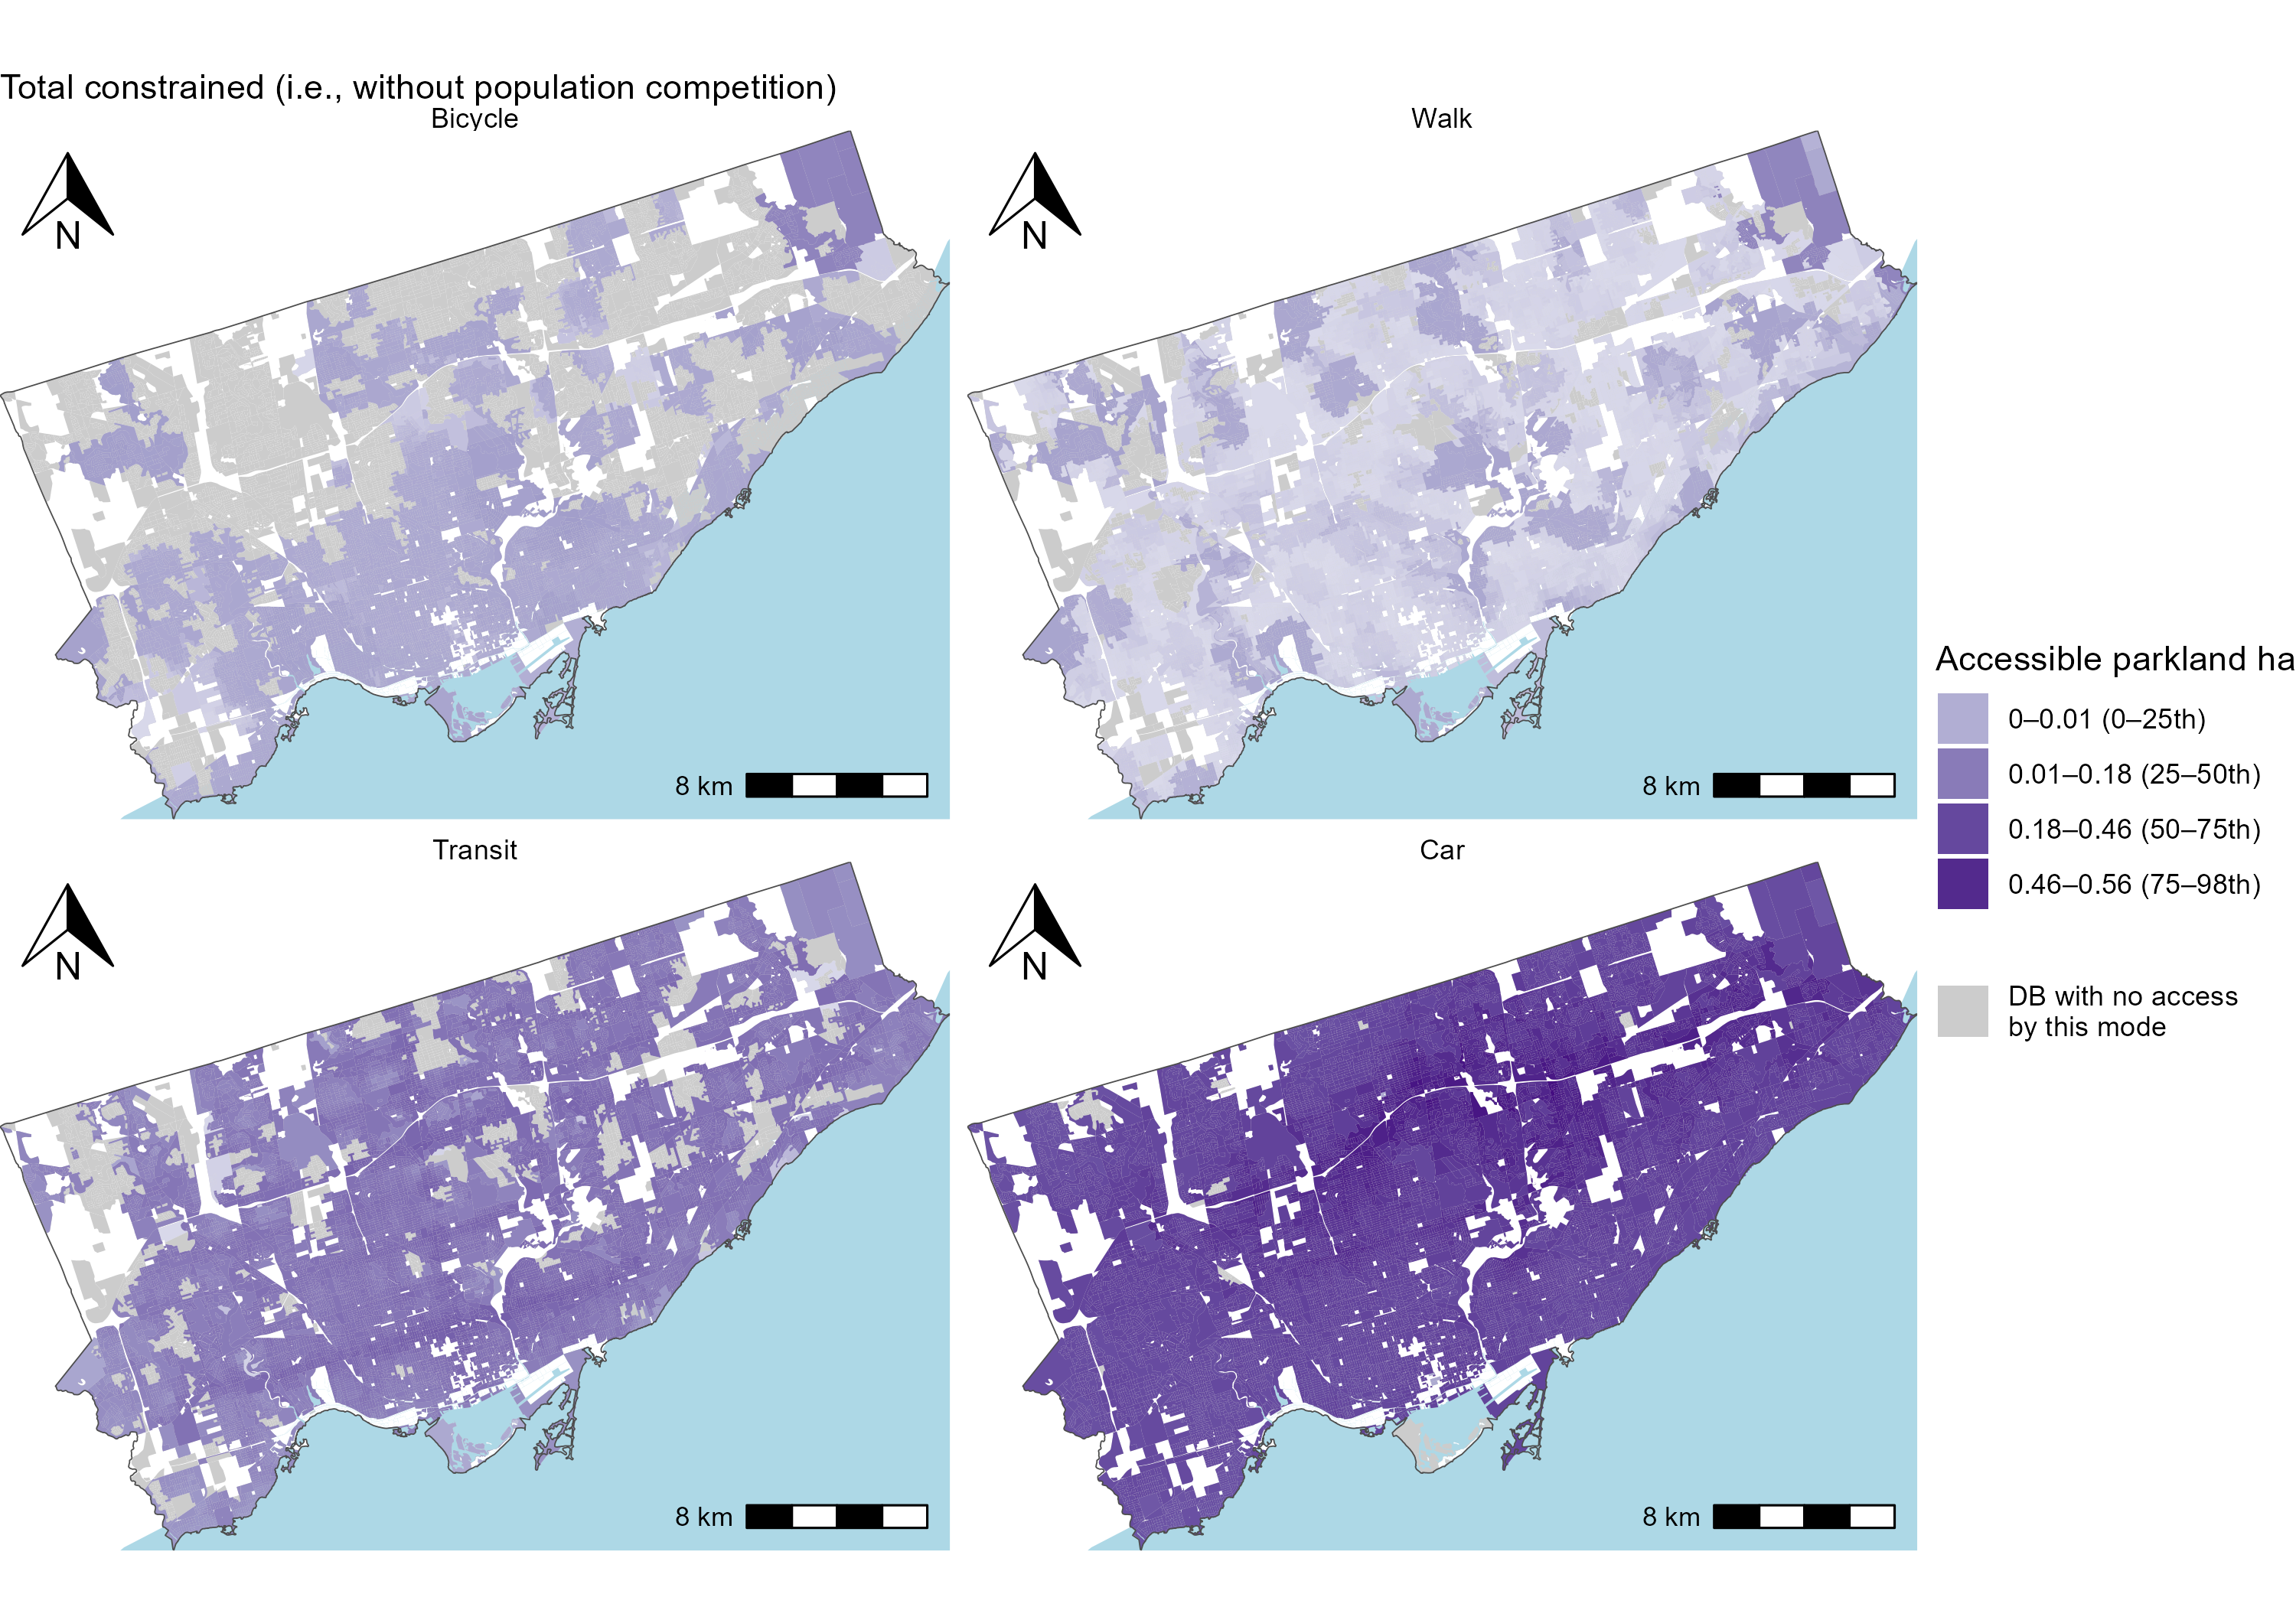
\includegraphics[width=6in]{./data/figures/chp5-mm_parkland_total_conc_access_DB_plots} 

}

\caption{\label{fig:chp5-mm_parkland_concs_access_DB_plots}Multimodal accessibility to parkland area per DB as measured by the total constrained multimodal accessibility measure.}\label{fig:unnamed-chunk-76}
\end{figure}

As the system is constrained, values in the region can be discussed as proportions of the total parkland area in the region. The majority of parkland area (65\%) is calculated to be multimodally accessible for the car-using population, while 31\%, 3\% and 1\% of the remaining parkland is multimodally accessible by transit, cycling and walking populations respectively.

Recall: this allocation works by taking the sum of total parkland area, and allocating it to origins based on the mode's relative travel impedance to reachable parkland area. The proportion of the population using the mode does not enter the equation. Hence, as car and transit are the furthest reaching modes these modes dominate allocation. Furthermore: car populations are assumed to not be able to reach smaller parkland area, but despite this assumption, car still dominates allocation, in part because larger parkland area dominates the amount of total parkland area in the city: 9\% of the total parkland area is small (i.e., parkettes, small and medium parks) and the remaining 91\% is large (i.e., large, city and legacy parks).

\subsection{Mode-specific singly constrained multimodal accessibility}\label{mode-specific-singly-constrained-multimodal-accessibility}

The spatial pattern in Figure \ref{fig:chp5-mm_parkland_singly_conc_access_DB_plots} differs significantly from the total constrained measure. One notable distinction is that many DBs in the northern parts of the city report no cycling mode share for leisure trips, despite having population. Hence, under the singly constrained measure, DBs with a cycling mode share of zero are effectively excluded from competing for parkland area by that mode--resulting in zero multimodal accessibility values. These DBs see competition for the multimodal accessible parkland area between the remaining modal population.

\begin{figure}

{\centering 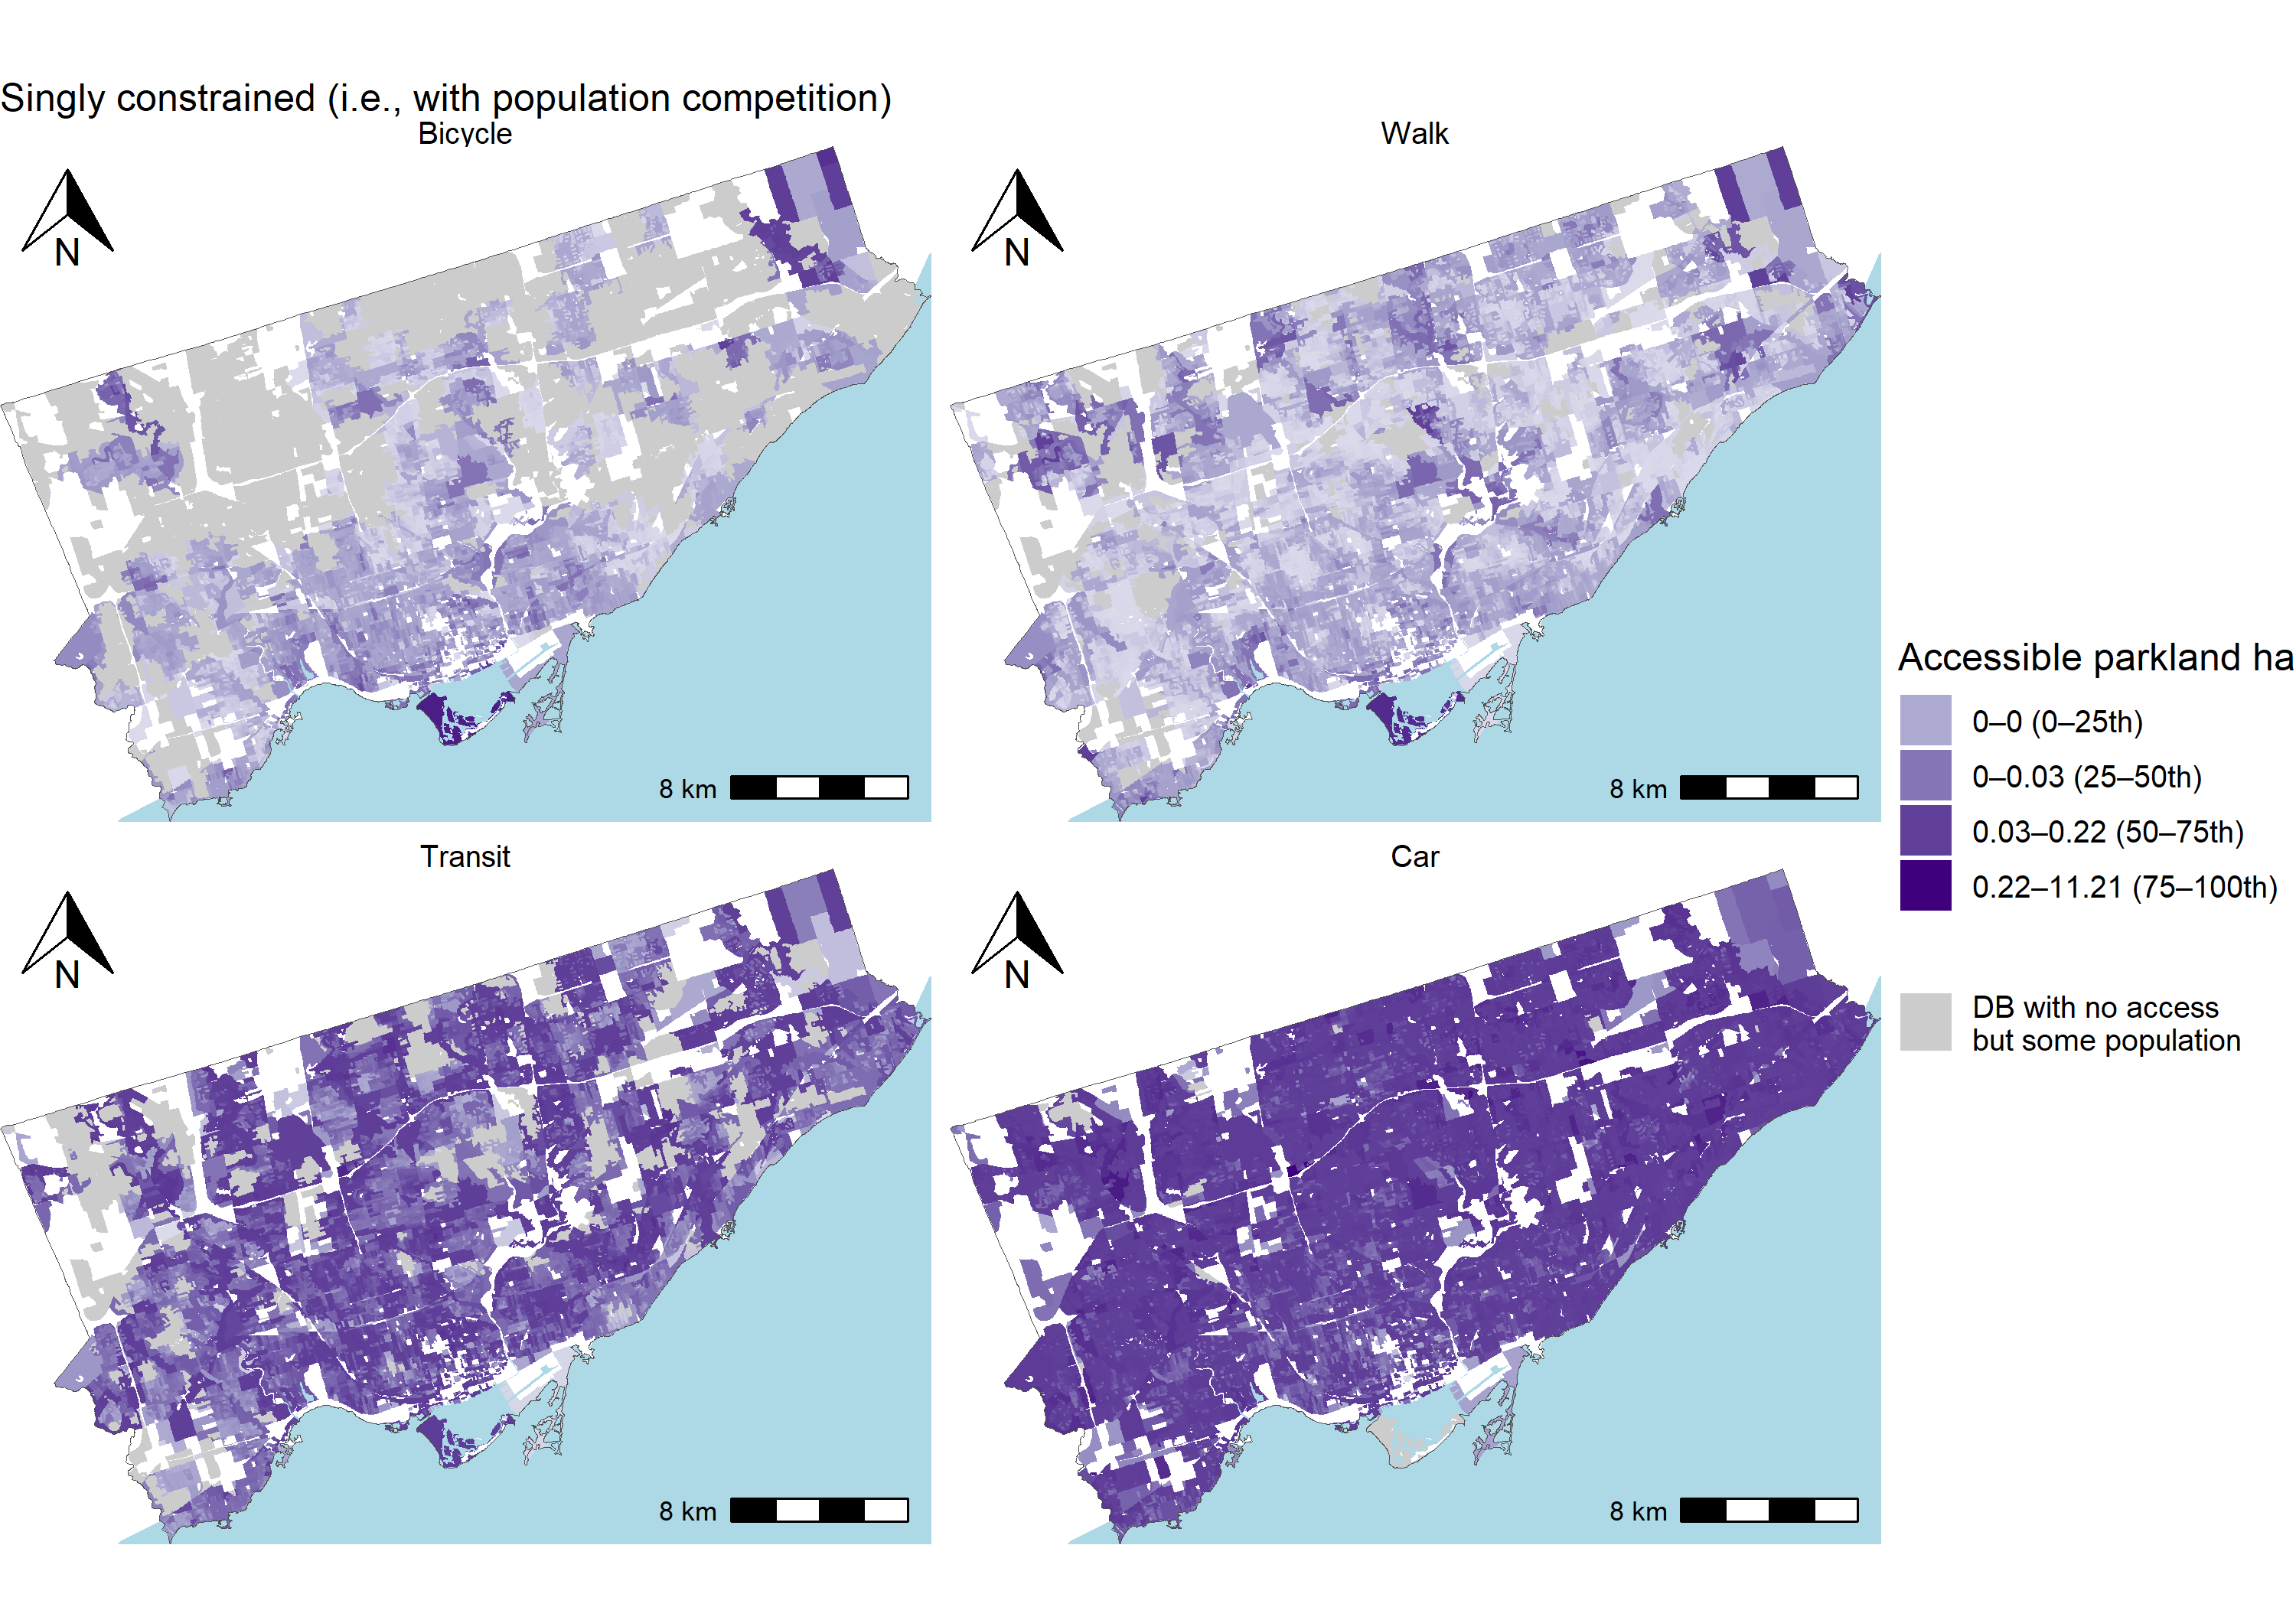
\includegraphics[width=6in]{./data/figures/chp5-mm_parkland_singly_conc_access_DB_plots} 

}

\caption{\label{fig:chp5-mm_parkland_singly_conc_access_DB_plots}Accessibility to parkland area per DB as measured by singly constrained multimodal accessibility.}\label{fig:unnamed-chunk-77}
\end{figure}

To faciliate comparison, Figure \ref{fig:chp5-mm_parkland_diff_conc_access_DB_plots} visualizes the difference between the singly constrained and total constrained accessibility values for each mode. Areas shaded in orange-red represent locations where the total constrained values are higher, indicating lower accessible parkland availability once competition is taken into account. These orange-to-red areas dominate much of the city, reflecting where competition across multiple modes reduces parkland allocation for a given mode group.

\begin{figure}

{\centering 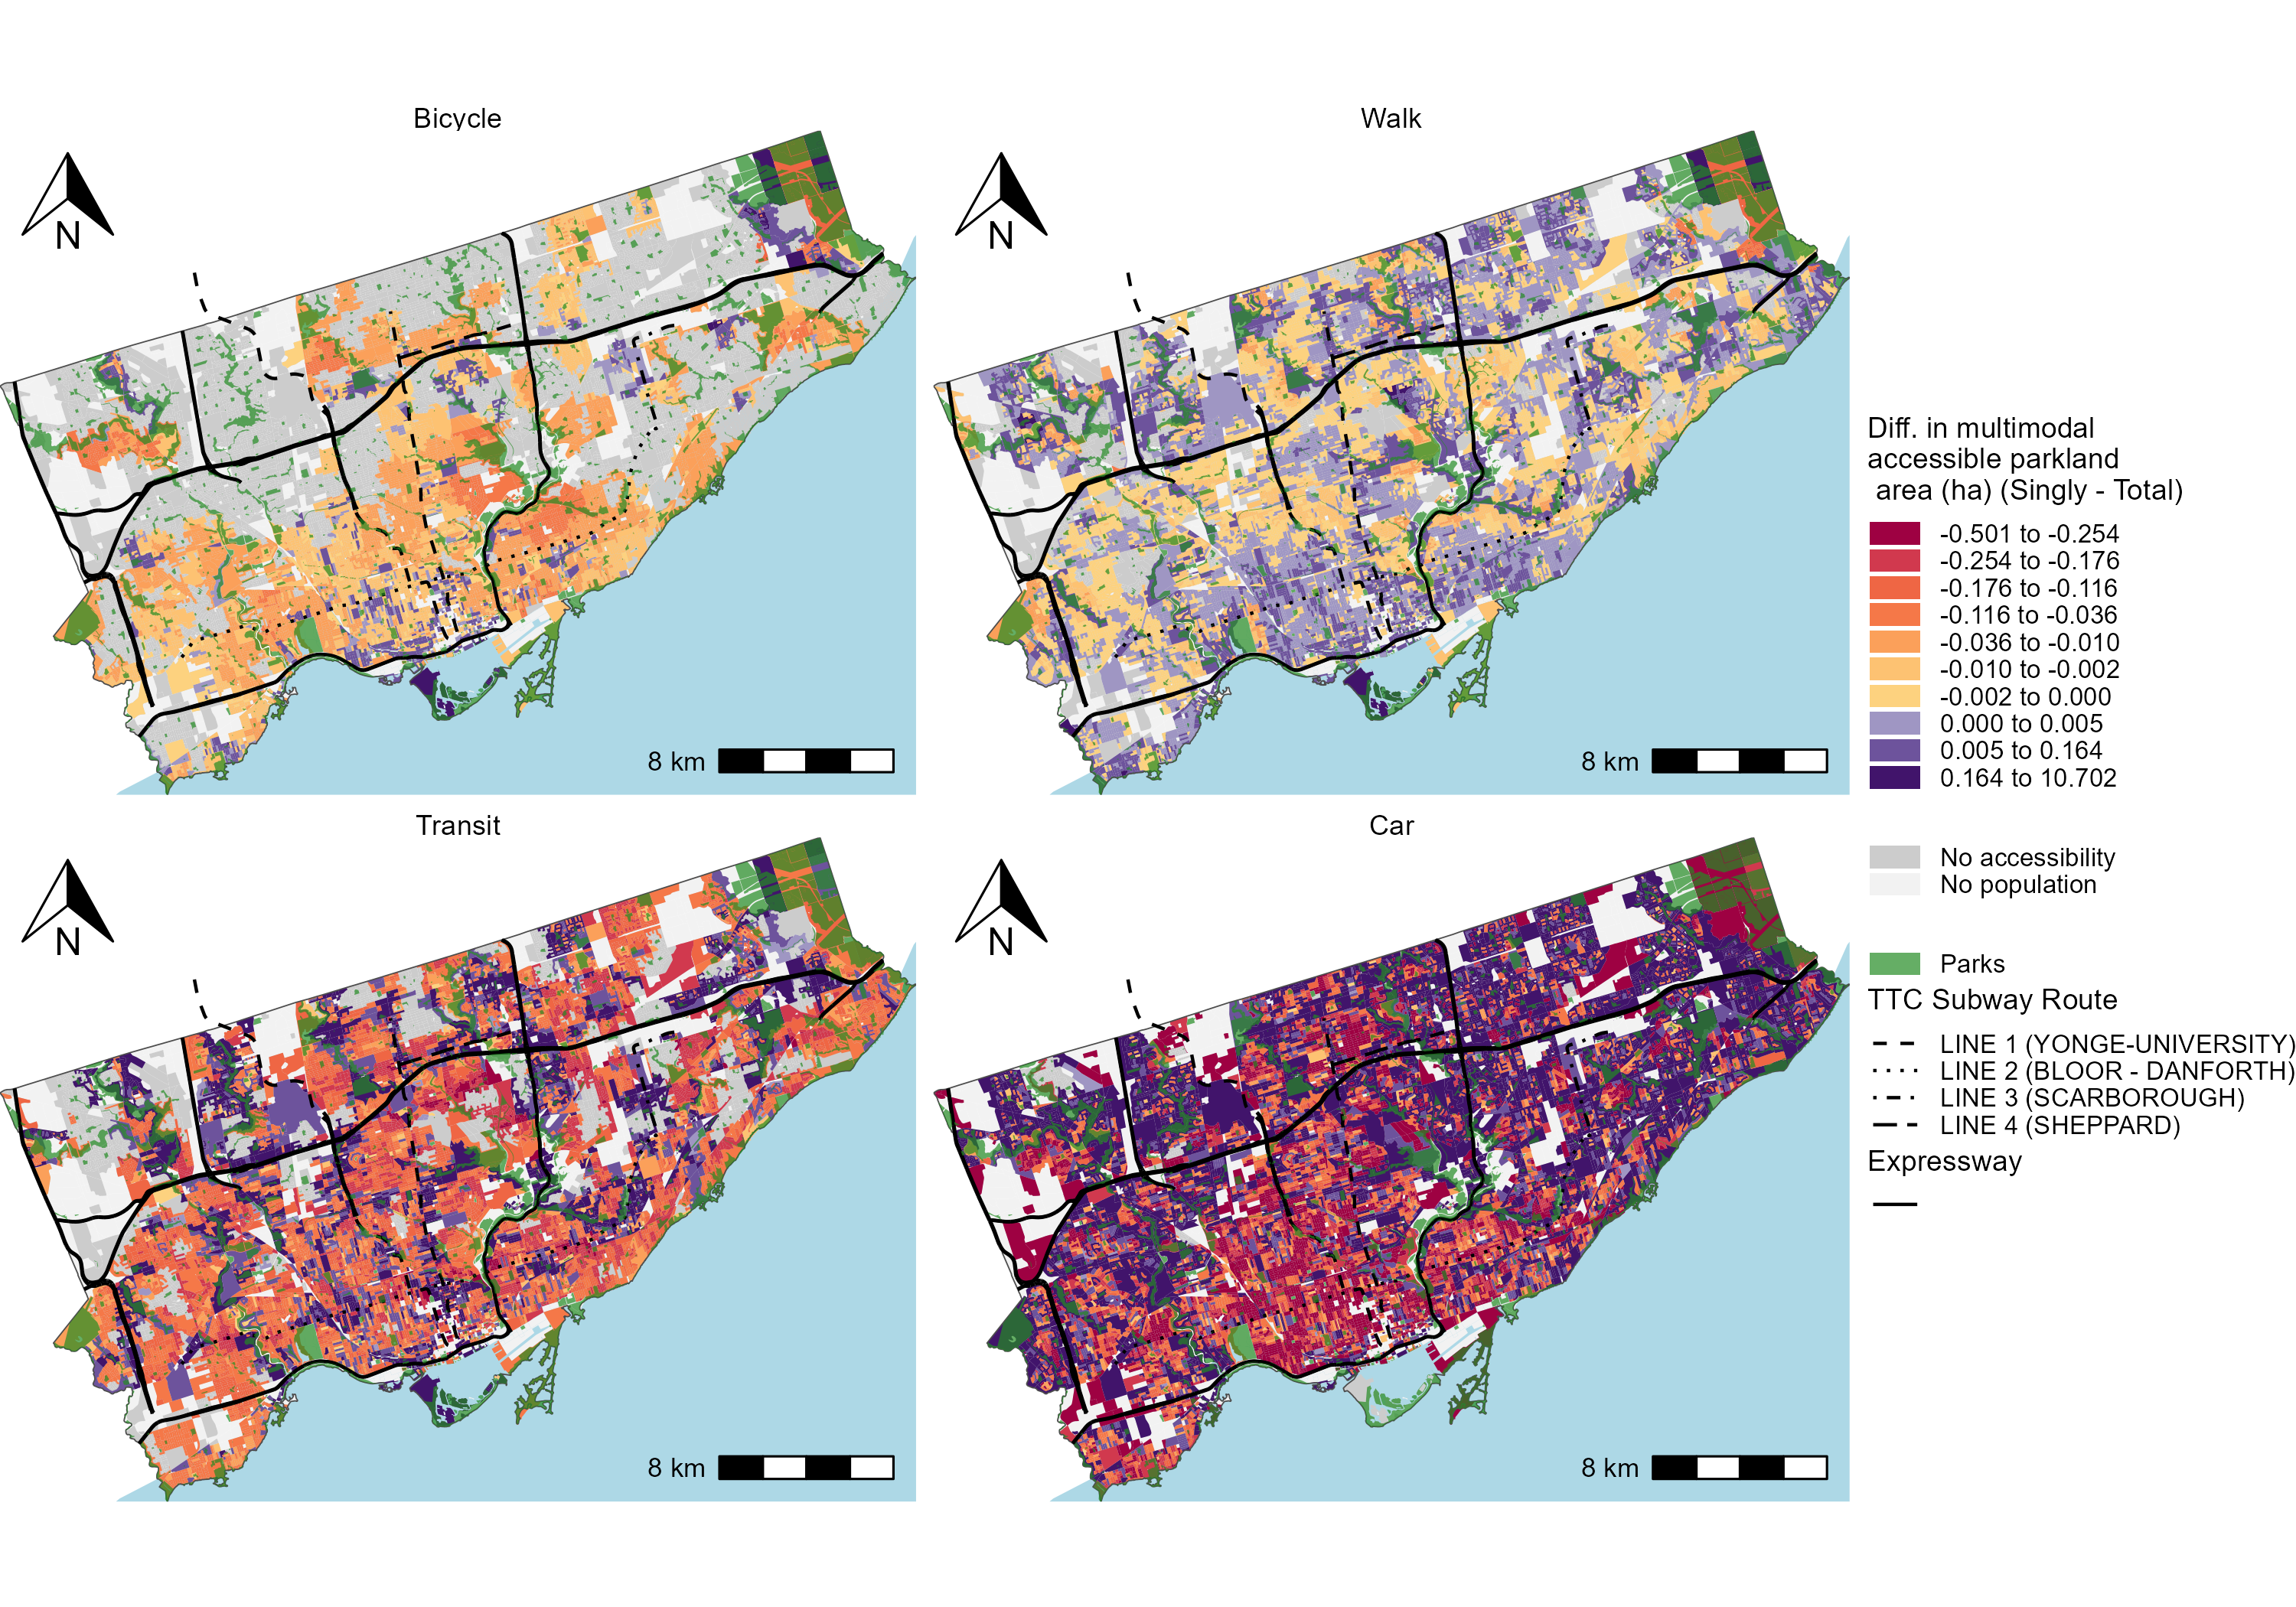
\includegraphics[width=6in]{./data/figures/chp5-mm_parkland_diff_conc_access_DB_plots} 

}

\caption{\label{fig:chp5-mm_parkland_diff_conc_access_DB_plots}Difference in singly constrained and total constrained multimodally accessible parkland area pe DB for each mode.}\label{fig:unnamed-chunk-78}
\end{figure}

In contrast, purple-shaded areas represent DBs where the singly constrained values are higher--indicating greater parkland accessibility when mode-specific demand is explicitly considered. This pattern is especially evident in the downtown core and in areas east of the expressway near the shoreline, particularly for walking, and to a lesser extent for cycling and transit. These are locations with high shares of non-car mode split, and as such, receive a greater allocation of parkland are using the singly constrained measure due to increased demand. Purple areas also emerge along the subway line for transit, and in neighbourhoods with relatively high cycling mode share. Additionally, for active and transit modes, purple zones tend to be present near smaller parks, which are assumed to be inaccessible by car (recall: methodological assumption). In these contexts, walking, cycling, and transit become more competitive than driving--especially in more suburban areas just outside the downtown.

As for the portion of DBs--those that are shaded orange-red--these demosntrate the opposite trend: where total constrained values are higher (i.e., values are higher when population demand is not considered). Car mode has the most intensely red DBs, in part because this mode yields the highest accessible parkland area due to its exceptionally low travel impedance. In areas where car mode share is relatively lower--such as near the downtown core where mode-share of non-car modes is higher--this helps to translate into much lower accessibility under the singly constrained measure relative to the total constrained values.

This comparison of multimodal accessibility results highlights the impact that considering local demand has in shaping results. The consideration of multimodal population competition introduces an additional layer of complexity: not only does parkland supply vary across the city, but so does the presence and proportion of different mode-using populations at each DB. The consider of modal population demand in addition to potential travel to parkland supply leads to patterns of accessibility that are more locally sensitive than those produced by the total constrained measure.

\subsection{Constrained multimodal accessibility per mode-using capita}\label{constrained-multimodal-accessibility-per-mode-using-capita}

As in Chapter 4, it is useful to express accessibility results as parkland area per capita, enabling comparisons to tangible and established benchmarks. For instance, Toronto Parkland Strategy's illustrative categories: 2 sqm (the space of a hula hoop), 4 sqm (beneath a patio umbrella), 12 sqm (within a bus shelter), and 28 sqm (the canopy of a mid-sized tree). The Strategy also identifies 12 sqm per capita as a threshold indicating parkland need (City of Toronto, 2019). These categories are used in this section, in addition to an additional category of 50 sqm, the canopy of a large tree, to further distinguish areas that capture a large amount of multimodally accessible parkland area. And as an additional note, values are not aggregated to another zoning system like done in Chapter 4, for the sake of brevity. Results are only discussed at the DB-level. However, aggregating at higher spatial resolutions while maintaining interpretability of units is possible under the multimodal constrained framework, like in the unimodal example.

Beginning first with a comparison of the total and singly constrained values for motorised modes, Figure \ref{fig:chp5-mm_parkland_motorised_per_capita_conc_access_DB_plots} displays the per mode-using capita multimodal accessible parkland for transit and car.

\begin{figure}

{\centering 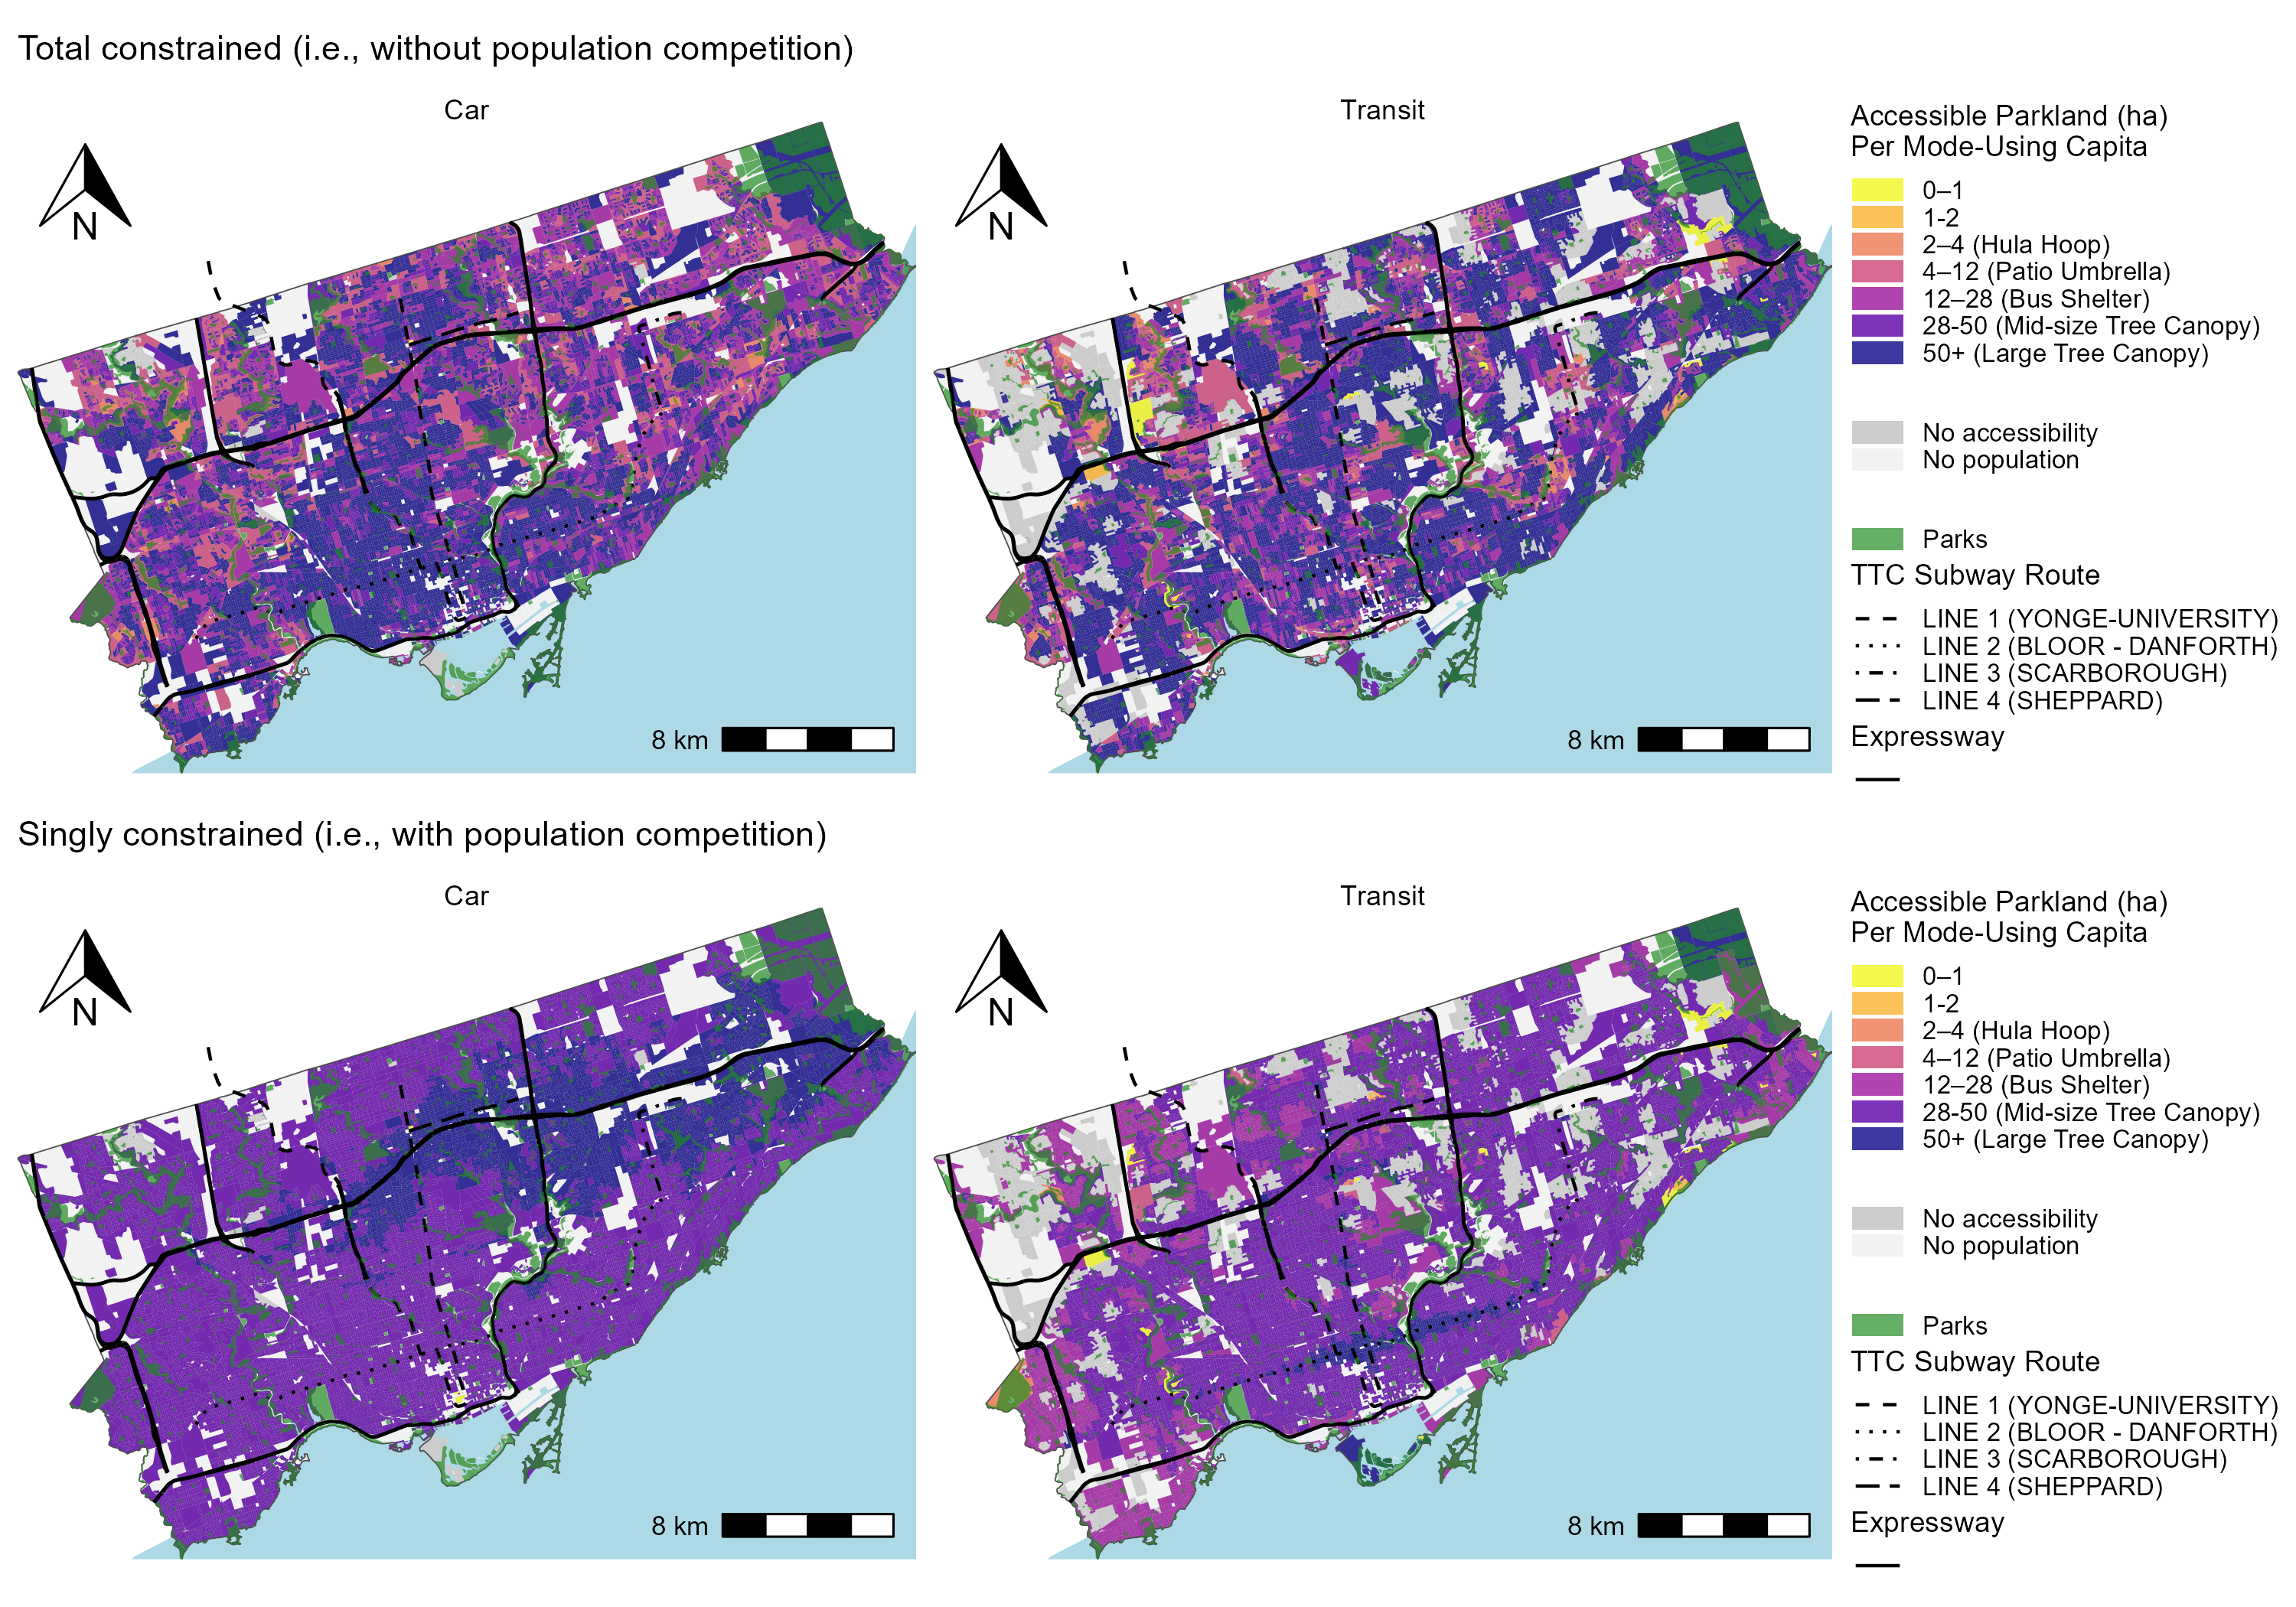
\includegraphics[width=6in]{./data/figures/chp5-mm_parkland_motorised_per_capita_conc_access_DB_plots} 

}

\caption{Total constrained (top) and singly constrained (bottom) multimodal accessibility to parkland area per mode-using capita for motorized modes.\label{fig:chp5-mm_parkland_motorised_per_capita_conc_access_DB_plots}}\label{fig:unnamed-chunk-79}
\end{figure}

Referring first to the total constrained values in Figure \ref{fig:chp5-mm_parkland_motorised_per_capita_conc_access_DB_plots}, values are exceptionally high for both modes; median of 60.14 and 50.39 sqm per capita for car and transit, with the vast majority of DBs exceeding the 12 sqm threshold. For the car mode, the highest total constrained per capita values occur within the center of the city (i.e., radiating outward from downtown). This reflects the low travel impedance and city-wide reach of the car-based infrastructure: DBs that are centrally located can access a large portion of the city's parkland quickly and efficiently. This aligns with the logic of the total constrained measure: if a park can be reached, it is allocated a portion of the total parkland area--and faster modes accumulate more portions relative to slower modes, irrespective of \emph{how many mode-users of each type of mode} there are competing. Transit per capita total constrained multimodal accessibility values also appear relatively high, though its spatial pattern is less spatially distinct than that of car. Despite not matching the car's travel `efficiency', transit's travel impedance is still relatively low (i.e., far reaching) and connected enough to parkland supply such that the result is substantial accessible parkland area across much of the city. Areas in the city that result in lower transit scores are the result of the travel impedance advantage of other modes and/or lower relative supply of parkland area.

Like the total constrained values, the singly constrained values in Figure \ref{fig:chp5-mm_parkland_motorised_per_capita_conc_access_DB_plots} are also exceptionally high. Car- and transit-using populations have median per capita accessible parkland of 45.88 and 32.2 sqm, respectively--both tending to far exceeding the 12 sqm threshold. For the car mode, the highest per capita accessibility is concentrated east of downtown and in the city's northeast, near the expressways. These areas benefit from both car-specific infrastructure (i.e., expressway reachability at high speeds) and large parkland areas, as well as a higher proportion of car users. For the transit-using population, the highest values appear along major subway corridors (especially Line 2), where both transit service levels and transit mode share are high. This reflects how mode-specific population demand and network coverage together influence per capita access patterns using the singly constrained measure.

What's interesting is how closely the singly constrained per capita values for the motorised modes mirror the raw total constrained patterns for those same modes (bottom row of Figure \ref{fig:chp5-mm_parkland_concs_access_DB_plots}); more so for car than for transit mode.

For transit, the highest values--both raw total constrained and per capita singly constrained--are concentrated along Line 2. This suggests that parkland in these areas along this line is not only highly reachable by transit, but also allocated at a rate that exceeds the effects of population competition. In other words, despite accounting for the number of transit users and their travel impedance, these areas still receive a proportionally high share of parkland--on par with proportions allocated assuming no modal population competition (i.e., total constrained accessibility). However, this proportionality does not extend in the same magnitude to other subway lines or high-frequency transit corridors (i.e., in areas with similarly high levels of total constrained accessibility). In those areas, singly constrained per capita values are not as high as along Line 2, implying that transit users are being out-competed by users of other modes. This highlights the nuance that considering not only the relative mode-specific travel impedance but also the modal competition provides to the results.

For car mode, the similarity between the singly constrained per capita values and the total constrained values is especially striking. Across the city, the two measures are highly correlated (Pearson correlation of 0.96). This strong relationship is unique to the car mode--no other mode shows a comparable relationship between per capita and raw accessibility values across either constrained measure.

But why may this be? Again, the singly constrained measure builds on the total constrained formulation by introducing an additional layer of restriction at a more detailed scale: the amount of parkland allocated from each park is constrained and allocation is based on modal population competition. In the case of the car mode, this layer of restriction ends up impacting results only minimally. Why? Because car travel impedance is so exceptionally low, and car-using populations are sufficently widespread meaning they consistently dominate in demanding larger shares of parkland area from each park. As a result, the car mode not only reaches more parkland than other modes, but also retains a per capita share at nearly equivalent \emph{proportions} to what it would receive without any population competition--that is, amounts comparable to its total constrained amounts.

Moving onto non-motorised per capita multimodal accessibility: Figure \ref{fig:chp5-mm_parkland_nonmotorised_per_capita_conc_access_DB_plots} visualises the corresponding maps. Overall, both non-motorized modes have much lower of accessible parkland sqm per capita than motorized mode users. The majority of DBs for walkers are below 12 sqm per capita by either measure (median of 0.43 and 0.39 sqm per capita for total and singly constrained measures respectively). Per capita values for cyclists are higher but more drastically different: DBs are allocated a per capita median rate of 2.88 for the singly constrained measure while the per capita total constrained rate presents a much more optimistic story with a median of 16.33 sqm per capita.

\begin{figure}

{\centering 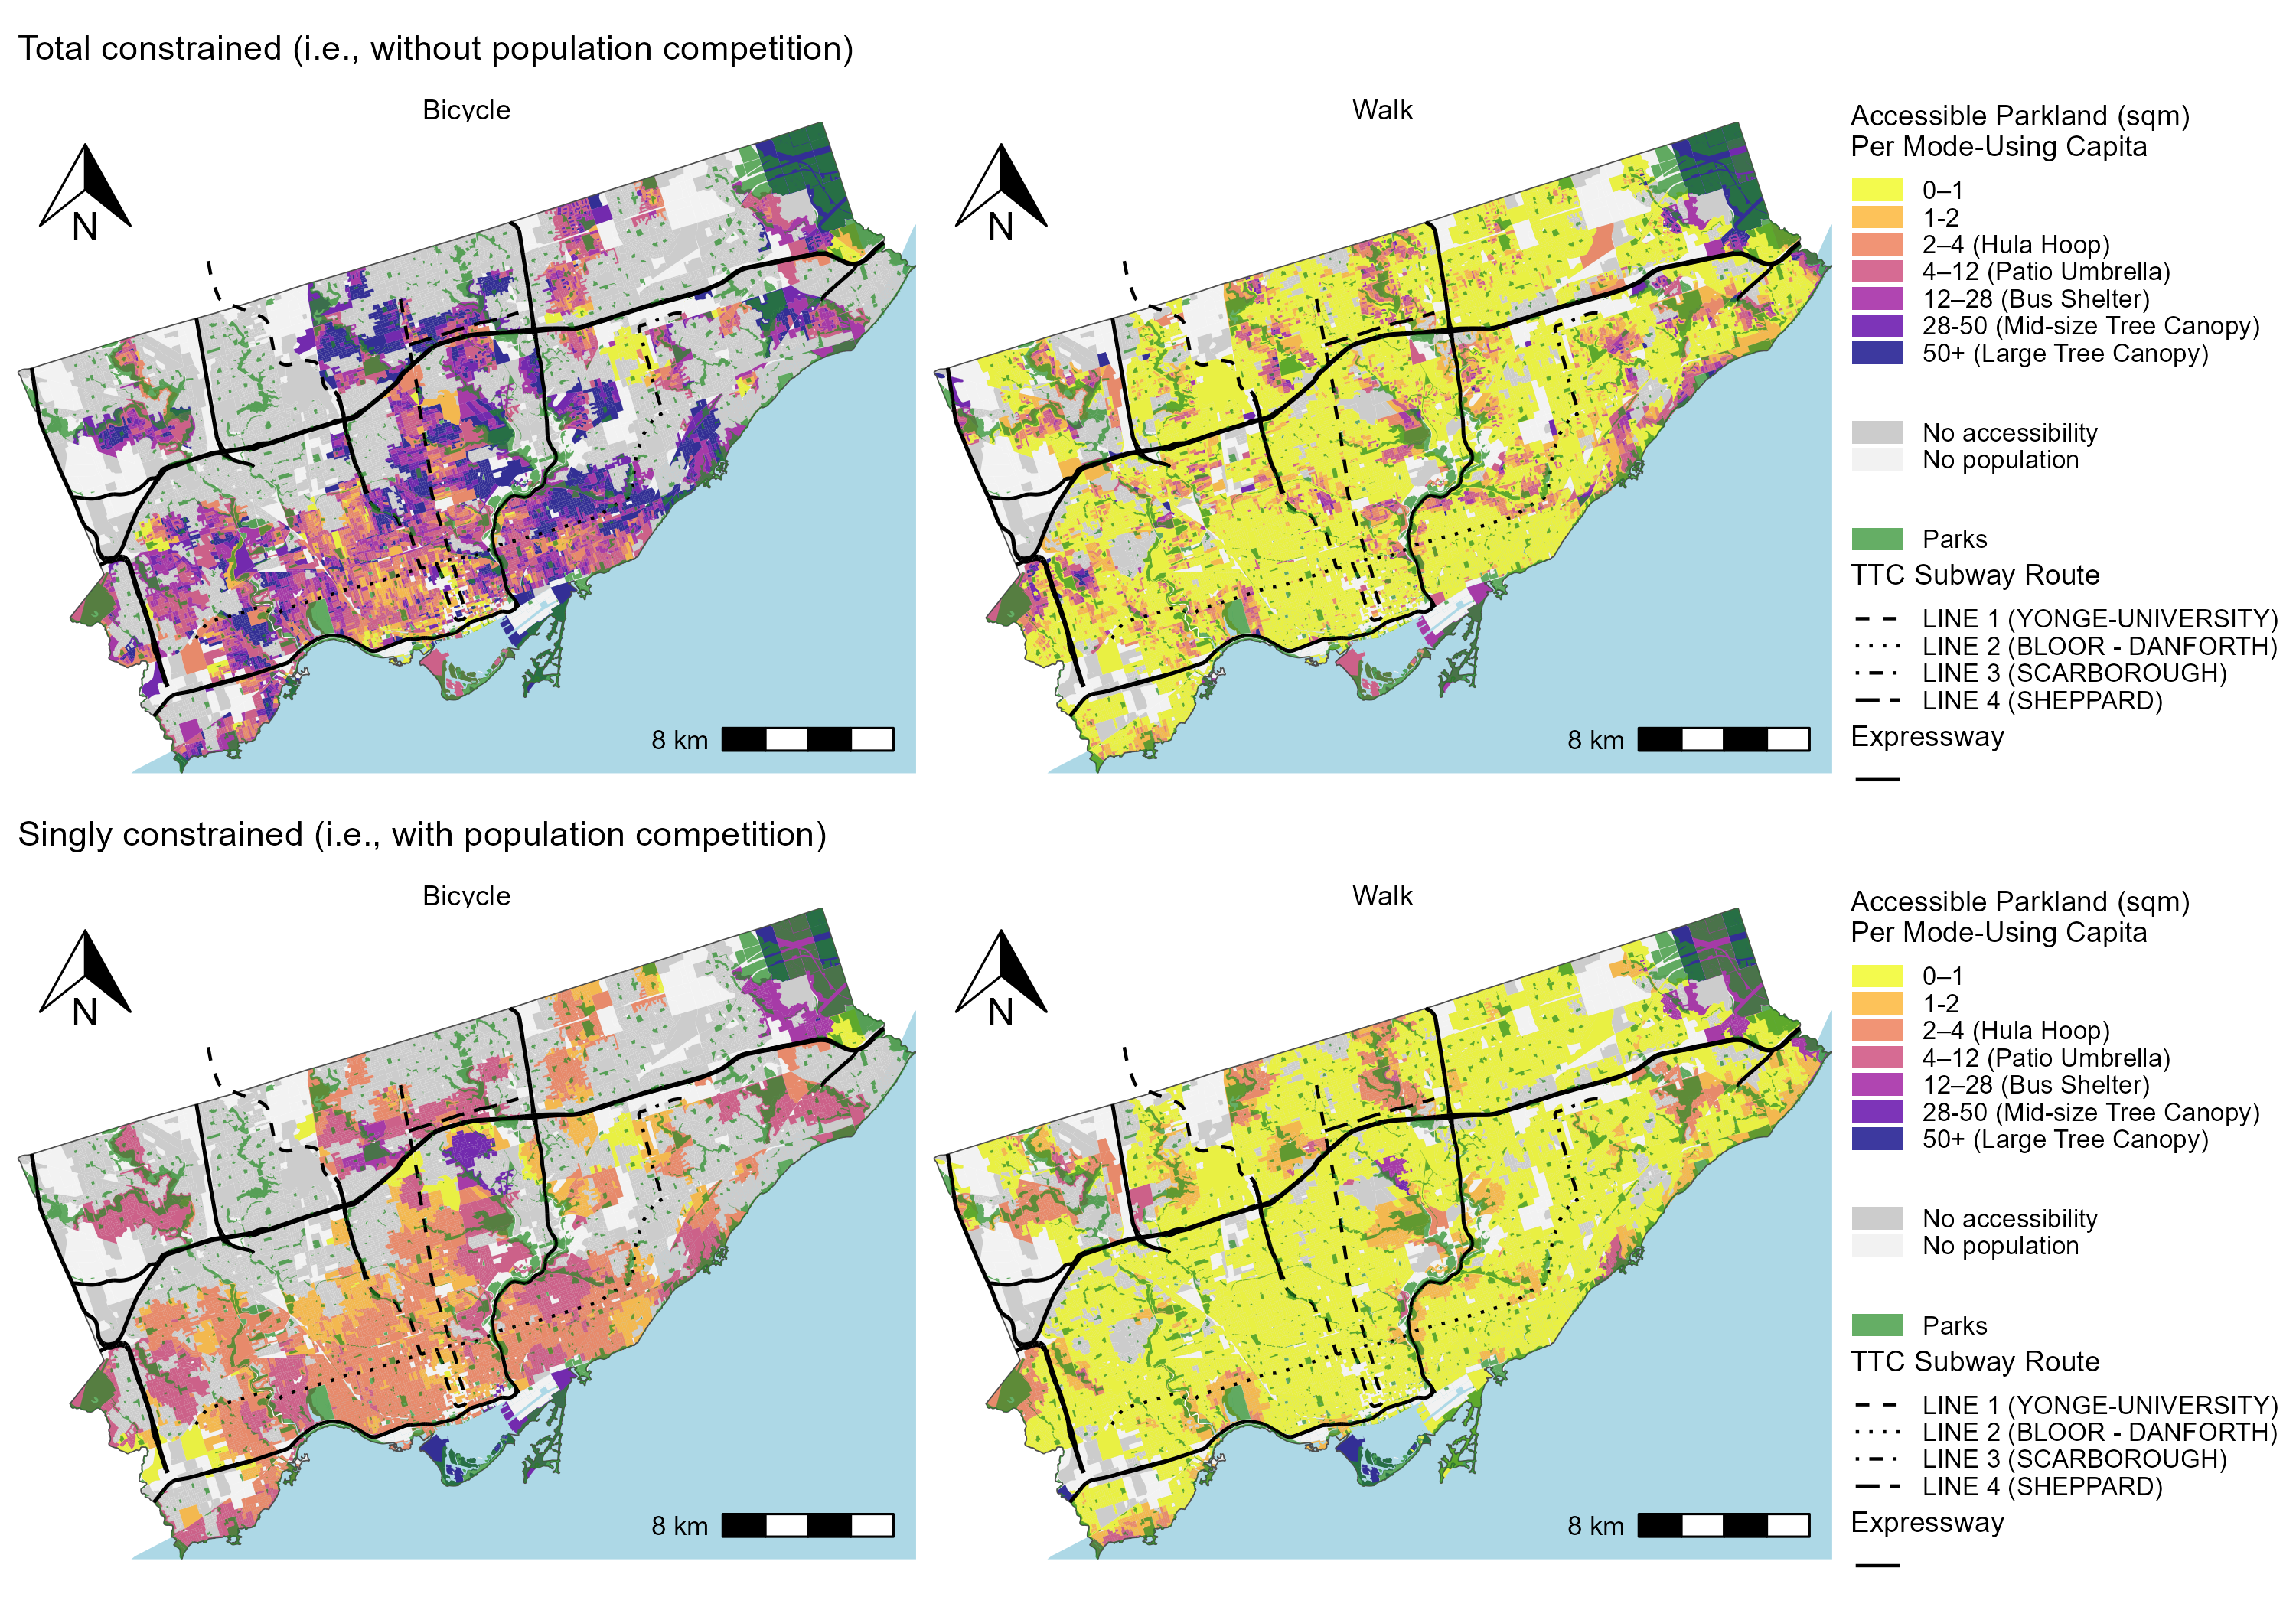
\includegraphics[width=6in]{./data/figures/chp5-mm_parkland_nonmotorised_per_capita_conc_access_DB_plots} 

}

\caption{\label{fig:chp5-mm_parkland_nonmotorised_per_capita_conc_access_DB_plots} Total constrained (top) and singly constrained (bottom) multimodal accessibility to parkland area per mode-using capita for non-motorized modes}\label{fig:unnamed-chunk-81}
\end{figure}

At first glance, the per capita walking plots in
Figure \ref{fig:chp5-mm_parkland_nonmotorised_per_capita_conc_access_DB_plots} appear
quite similar, and in fact show somewhat of a correlation between total and singly constrained values (0.35), the strongest relationship between per capita rates than for any other mode. However, readers should note that the assumed 15-minute walking range is spatially limited and a binary travel impedance is very dramatic, meaning that even small spatial variations can lead to meaningful differences at a localised scale. High per capita values are concentrated almost exclusively in areas immediately adjacent to parks, whereas in the total constrained plots, pockets of high accessibility also appear a bit farther from park boundaries. This suggests that introducing modal competition eliminates localised walking multimodal accessibility peaks, especially in areas where walking-population is lower.

In contrast to per capita walking values, per capita multimodal accessibility by \emph{cycling} demonstrates large differences between the two constrained measures in \ref{fig:chp5-mm_parkland_nonmotorised_per_capita_conc_access_DB_plots}. The total constrained cycling plot displays a wider spatial distribution of higher values--particularly on the edges of areas of where cycling mode share is present. These areas are north of downtown and to the north east of downtown, with plentiful parkland area and a cycling population. However, these elevated per capita values are largely eliminated in the singly constrained plot, indicating that modal competition has a stronger dampening effect on the proportion of multimodal accessibility allocated to the cycling population. Due to the consideration of modal competition: many parks reachable by cycling are also reachable by \emph{faster} motorised modes with similar travel impedance and in larger magnitudes (cycling mode-share is small), resulting in relatively low levels of parkland allocation to cyclists in the singly constrained measure even when adjusted to their per capita proportions.

\section{Multimodal accessible population (to the parkland)}\label{multimodal-accessible-population-to-the-parkland}

The multimodal accessible population variant introduces a new framing for the accessibility analysis. Instead of a focus on how well origins by modal population are preforming from the perspective of \emph{multimodal accessible parkland area}, in this section how efficiently reachable are parks by different modes or the \emph{multimodal accessible population} is investigated. This can be interpreted as the park's `market potential' considering multimodal accessibility.

Recall that this approach uses the same \(ij\) travel impedance as before but incorporates mode shares arriving to leisure destinations from the 2022 TTS (Figure \ref{fig:chp3-mode_split_parks_plots}). These modal shares serve to represent the proportion of the population most likely to reach the park by each mode, framing parkland area as mode-specific supply--for example, reflecting the observed use of infrastructure like parking spaces for drivers or bike racks for cyclists.

Figure \ref{fig:chp5-pop_unconc_access_parks_allmodes_plots} shows the unconstrained accessibility to population by mode, while Figure \ref{fig:chp5-pop_total_access_parks_allmodes_plots} demonstrates the mode-specific multimodal total constrained accessibility measure. While both measures are proportional, the key advantage of the constrained measure is that the total sum of accessible population across all modes and parks equals the total 2021 Toronto CMA population: \(2,794,356\). Parks that are inaccessible by a given mode are shown in green.

\begin{figure}

{\centering 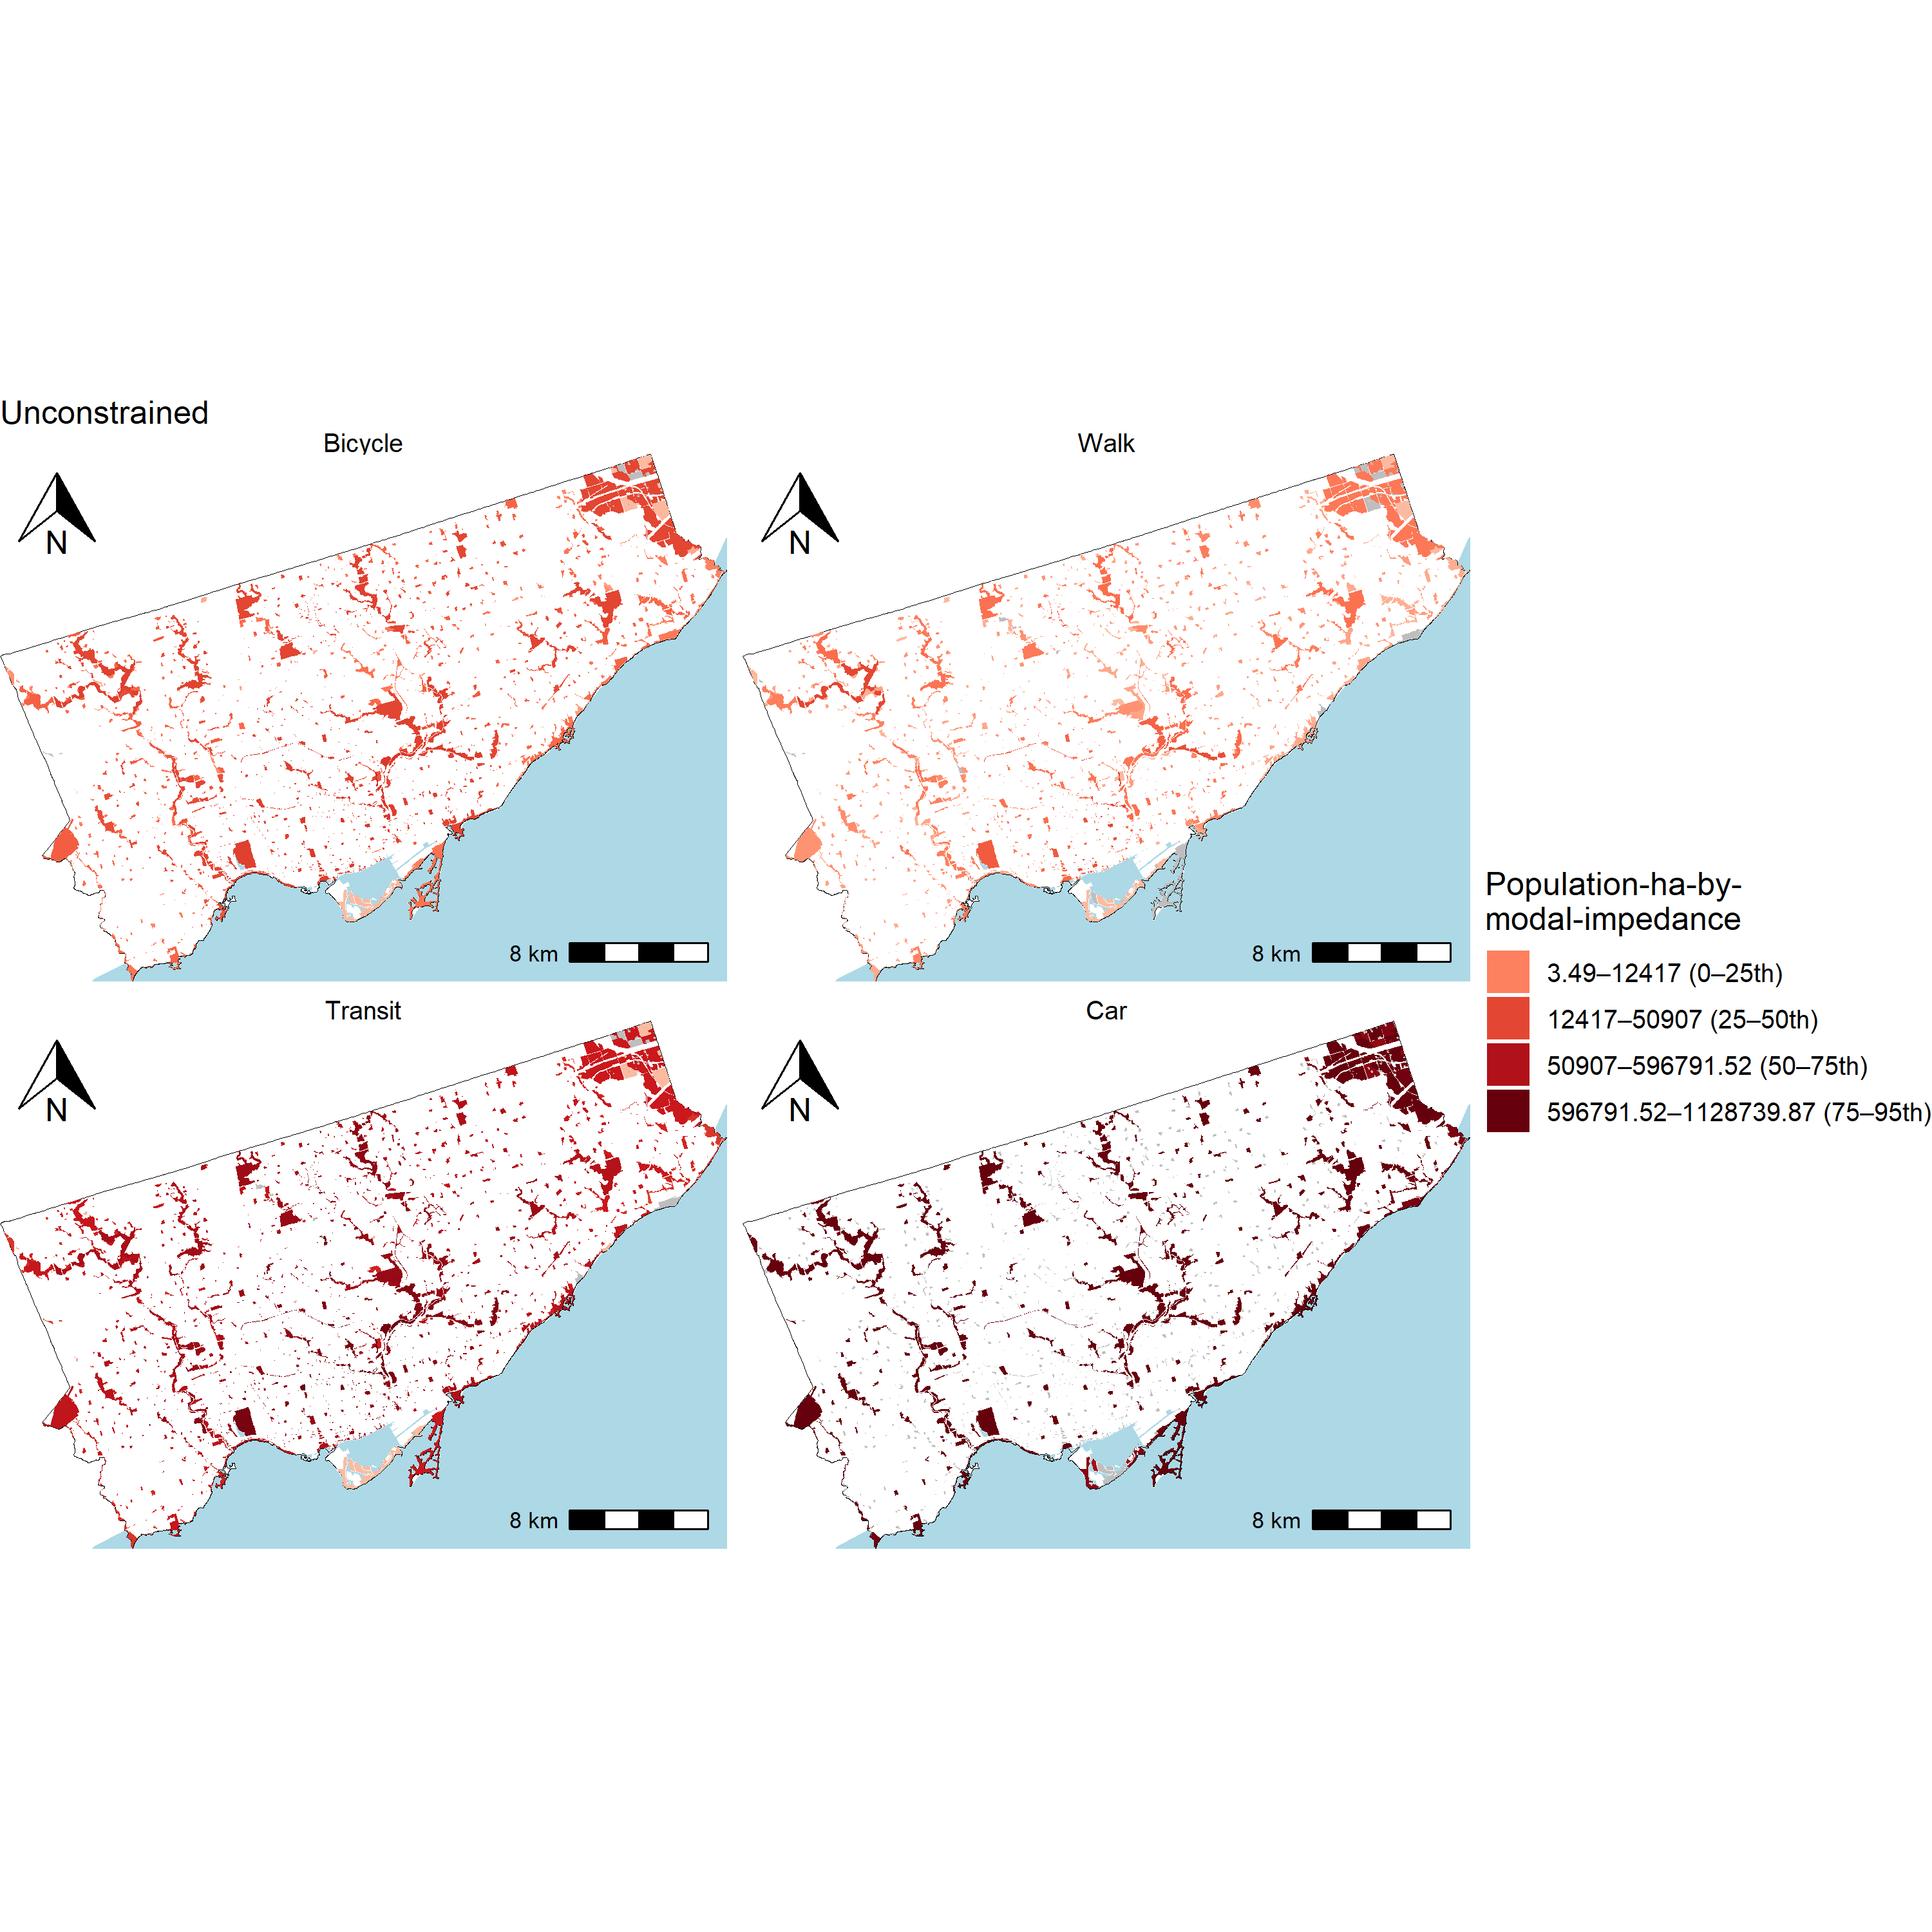
\includegraphics[width=6in]{./data/figures/chp5-pop_unconc_access_parks_allmodes_plots} 

}

\caption{\label{fig:chp5-pop_unconc_access_parks_allmodes_plots} Unconstrained accessible population-by-modal-impedance per park by multiple modes, i.e. market potential of each park by multiple modes.}\label{fig:unnamed-chunk-86}
\end{figure}

\begin{figure}

{\centering 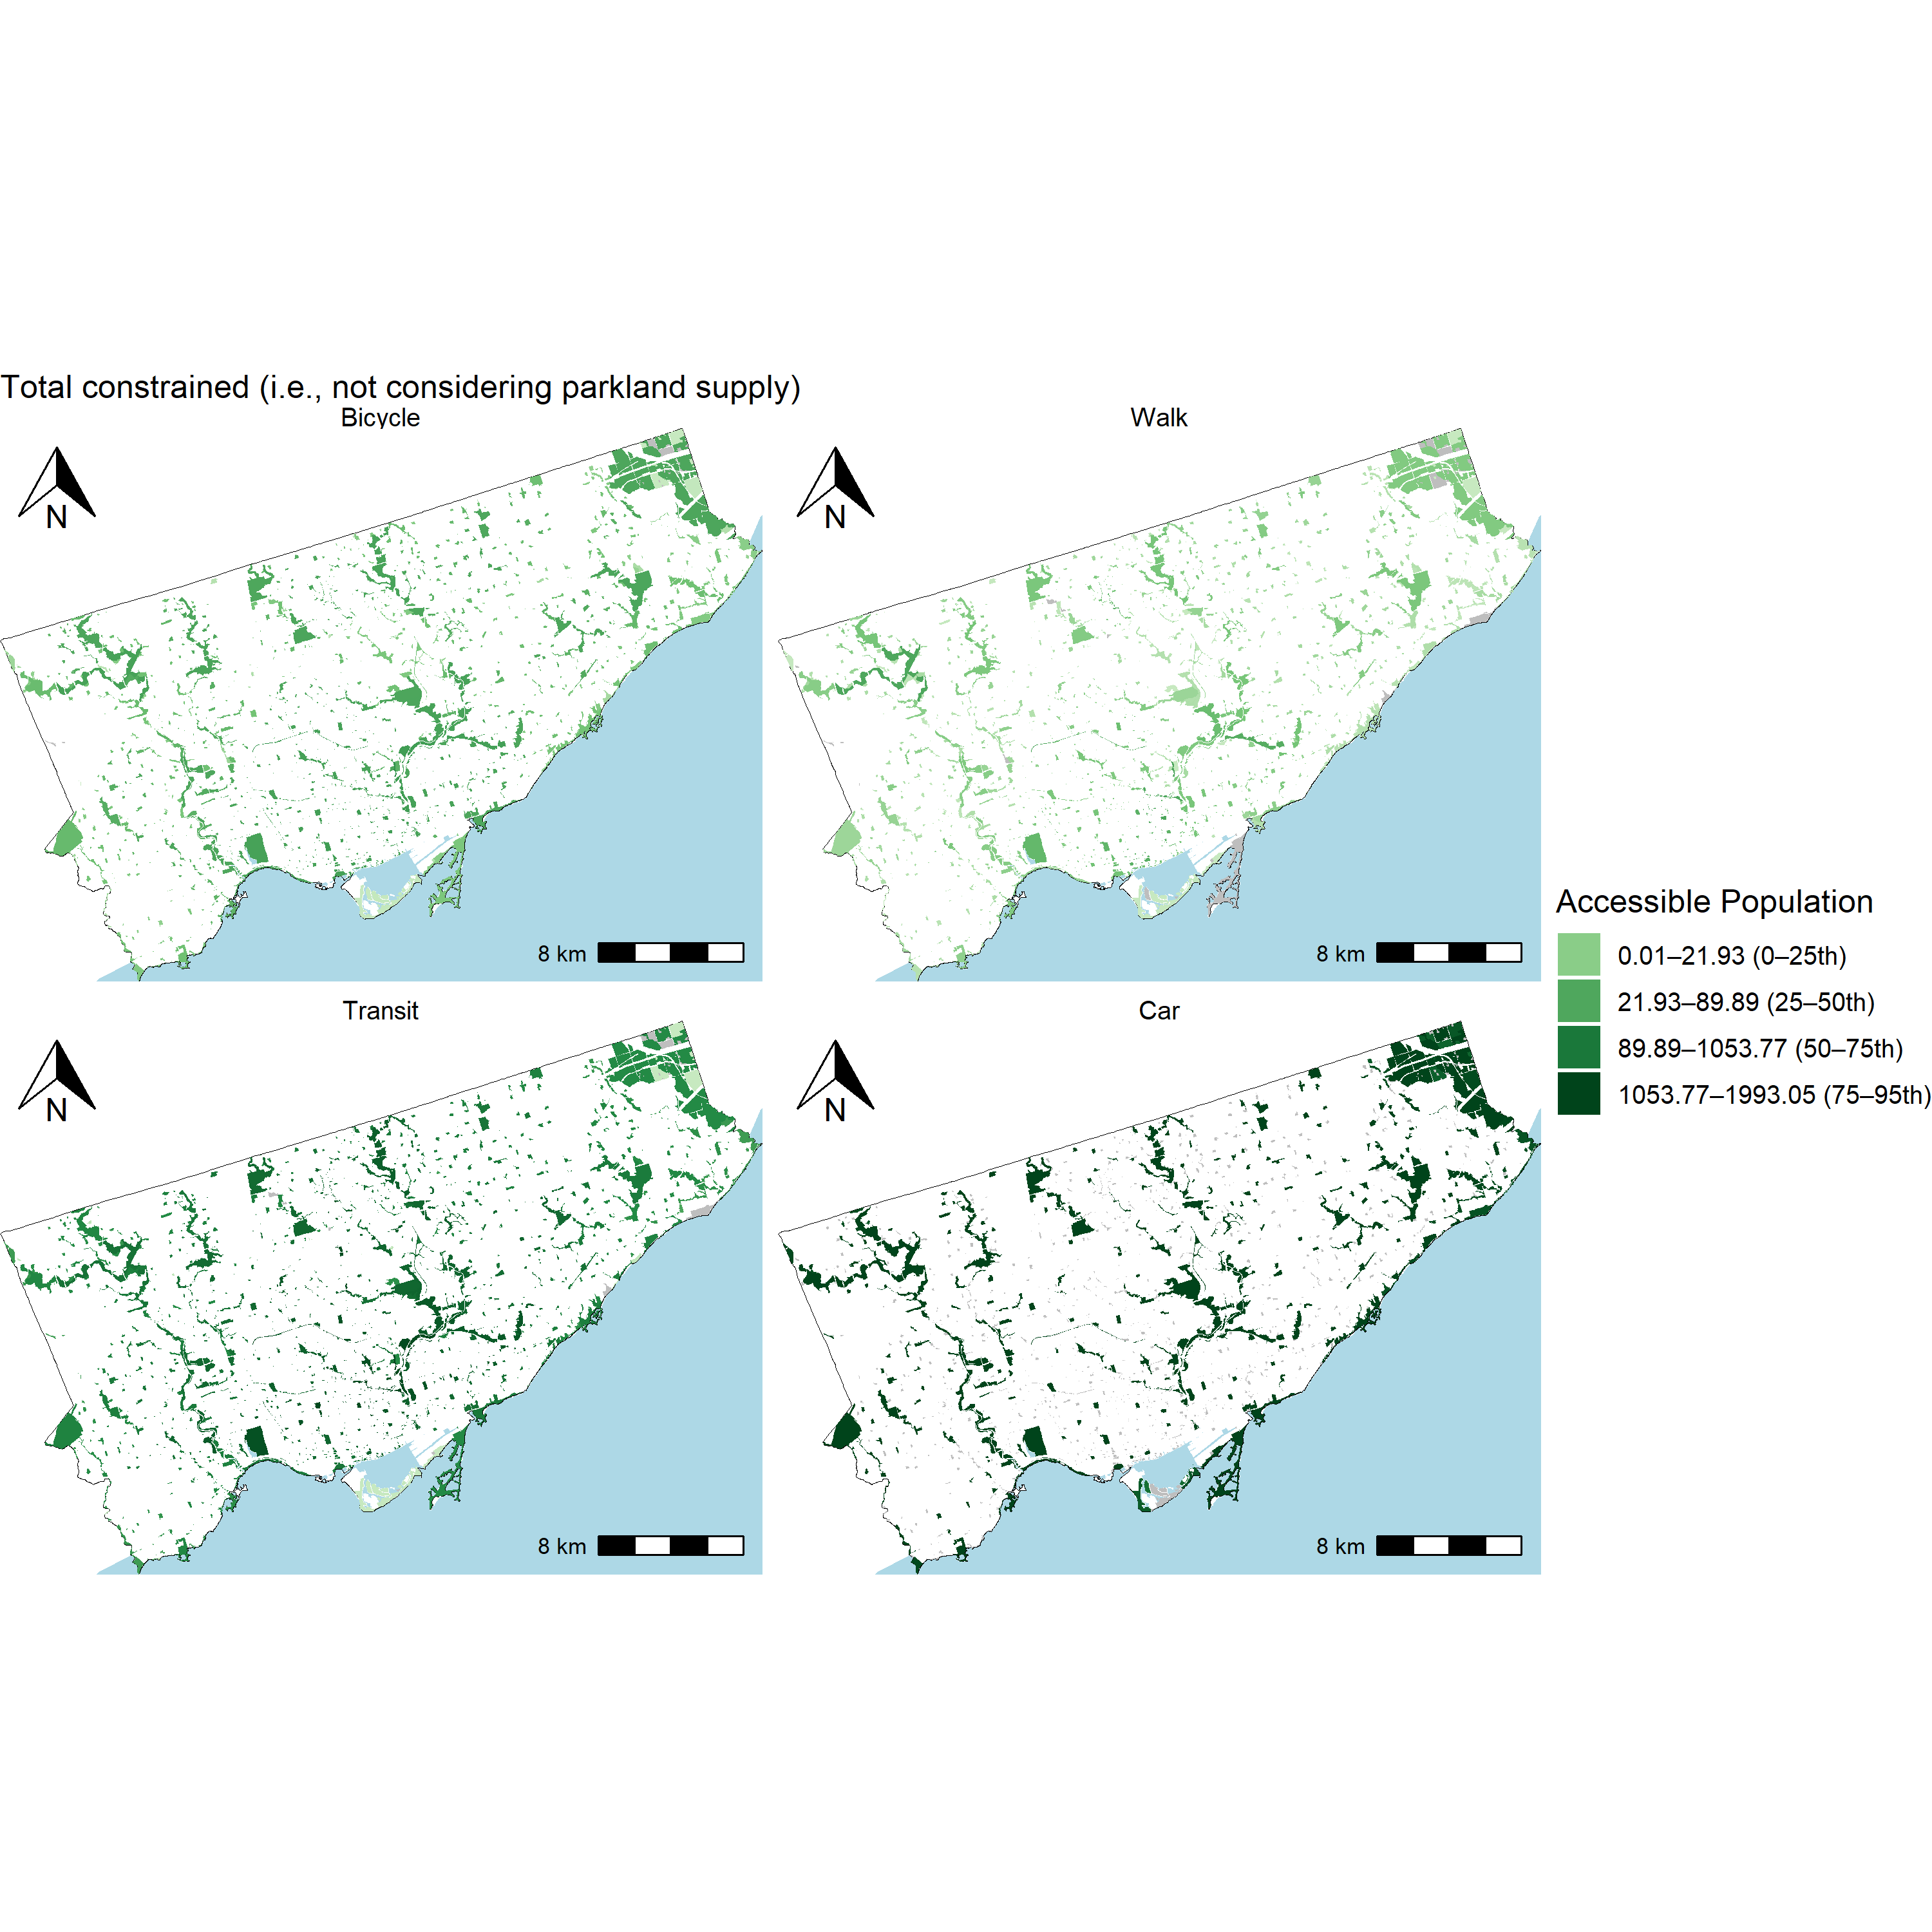
\includegraphics[width=6in]{./data/figures/chp5-pop_total_access_parks_allmodes_plots} 

}

\caption{\label{fig:chp5-pop_total_access_parks_allmodes_plots} Total constrained multimodal accessible population by mode per park.}\label{fig:unnamed-chunk-87}
\end{figure}

Figure \ref{fig:chp5-pop_unconc_access_parks_allmodes_plots} is the accessibility to people by mode calculated using the unconstrained measure and Figure \ref{fig:chp5-pop_total_access_parks_allmodes_plots} is the total constrained version of this measure, or the \emph{multimodal} accessibility to people by mode.

Interestingly: unlike in the accessible parkland area results (preceding section's discussion): transit emerges as the dominant mode in terms of multimodally accessible population. Specifically, 62\% of the total population is accessible from parks by transit, compared to 31\%, 6\% by car and 1\% by walking. This difference is a direct result of how the measure allocates total population: based on the modal travel impedance connecting people and parks, and then aggregated at the level of the park.

Transit--especially higher-order transit--is typically located in dense urban areas, which also contain many (albeit smaller) parks in Toronto's case. This spatial co-location makes transit highly efficient at connecting parks to large numbers of people, when only weighted by travel impedance (i.e., total constrained measure). By contrast, car-dominant populations is more present outside of the downtown area--in lower-density areas with fewer but larger parks. Even though car travel impedance is lower than transit, the co-location of parks in transit-using and population-dense areas appears to outweight this cost advantage.

From the perspective of walking and cycling modes at parks, they appear to capture relatively small shares of the multimodally accessible population than motorised modes. This is a similar ranking as in the multimodally accessible parkland area (previous sections) results. However, cycling-parkland-supply captures about two times more multimodally accessible population (6\%) than the cycling-mode using population captures multimodally accessible parkland (3\%). Why? For reasons similar reasons to transit: parks with more bike-specific park supply are in areas where population is higher-density.

Moving onto the singly constrained measure, Figure \ref{fig:chp5-pop_singly_access_parks_allmodes_plots} presents park level multimodally accessible population by mode-specific park supply. These results differ notably from those produced by the total constrained measure.

\begin{figure}

{\centering 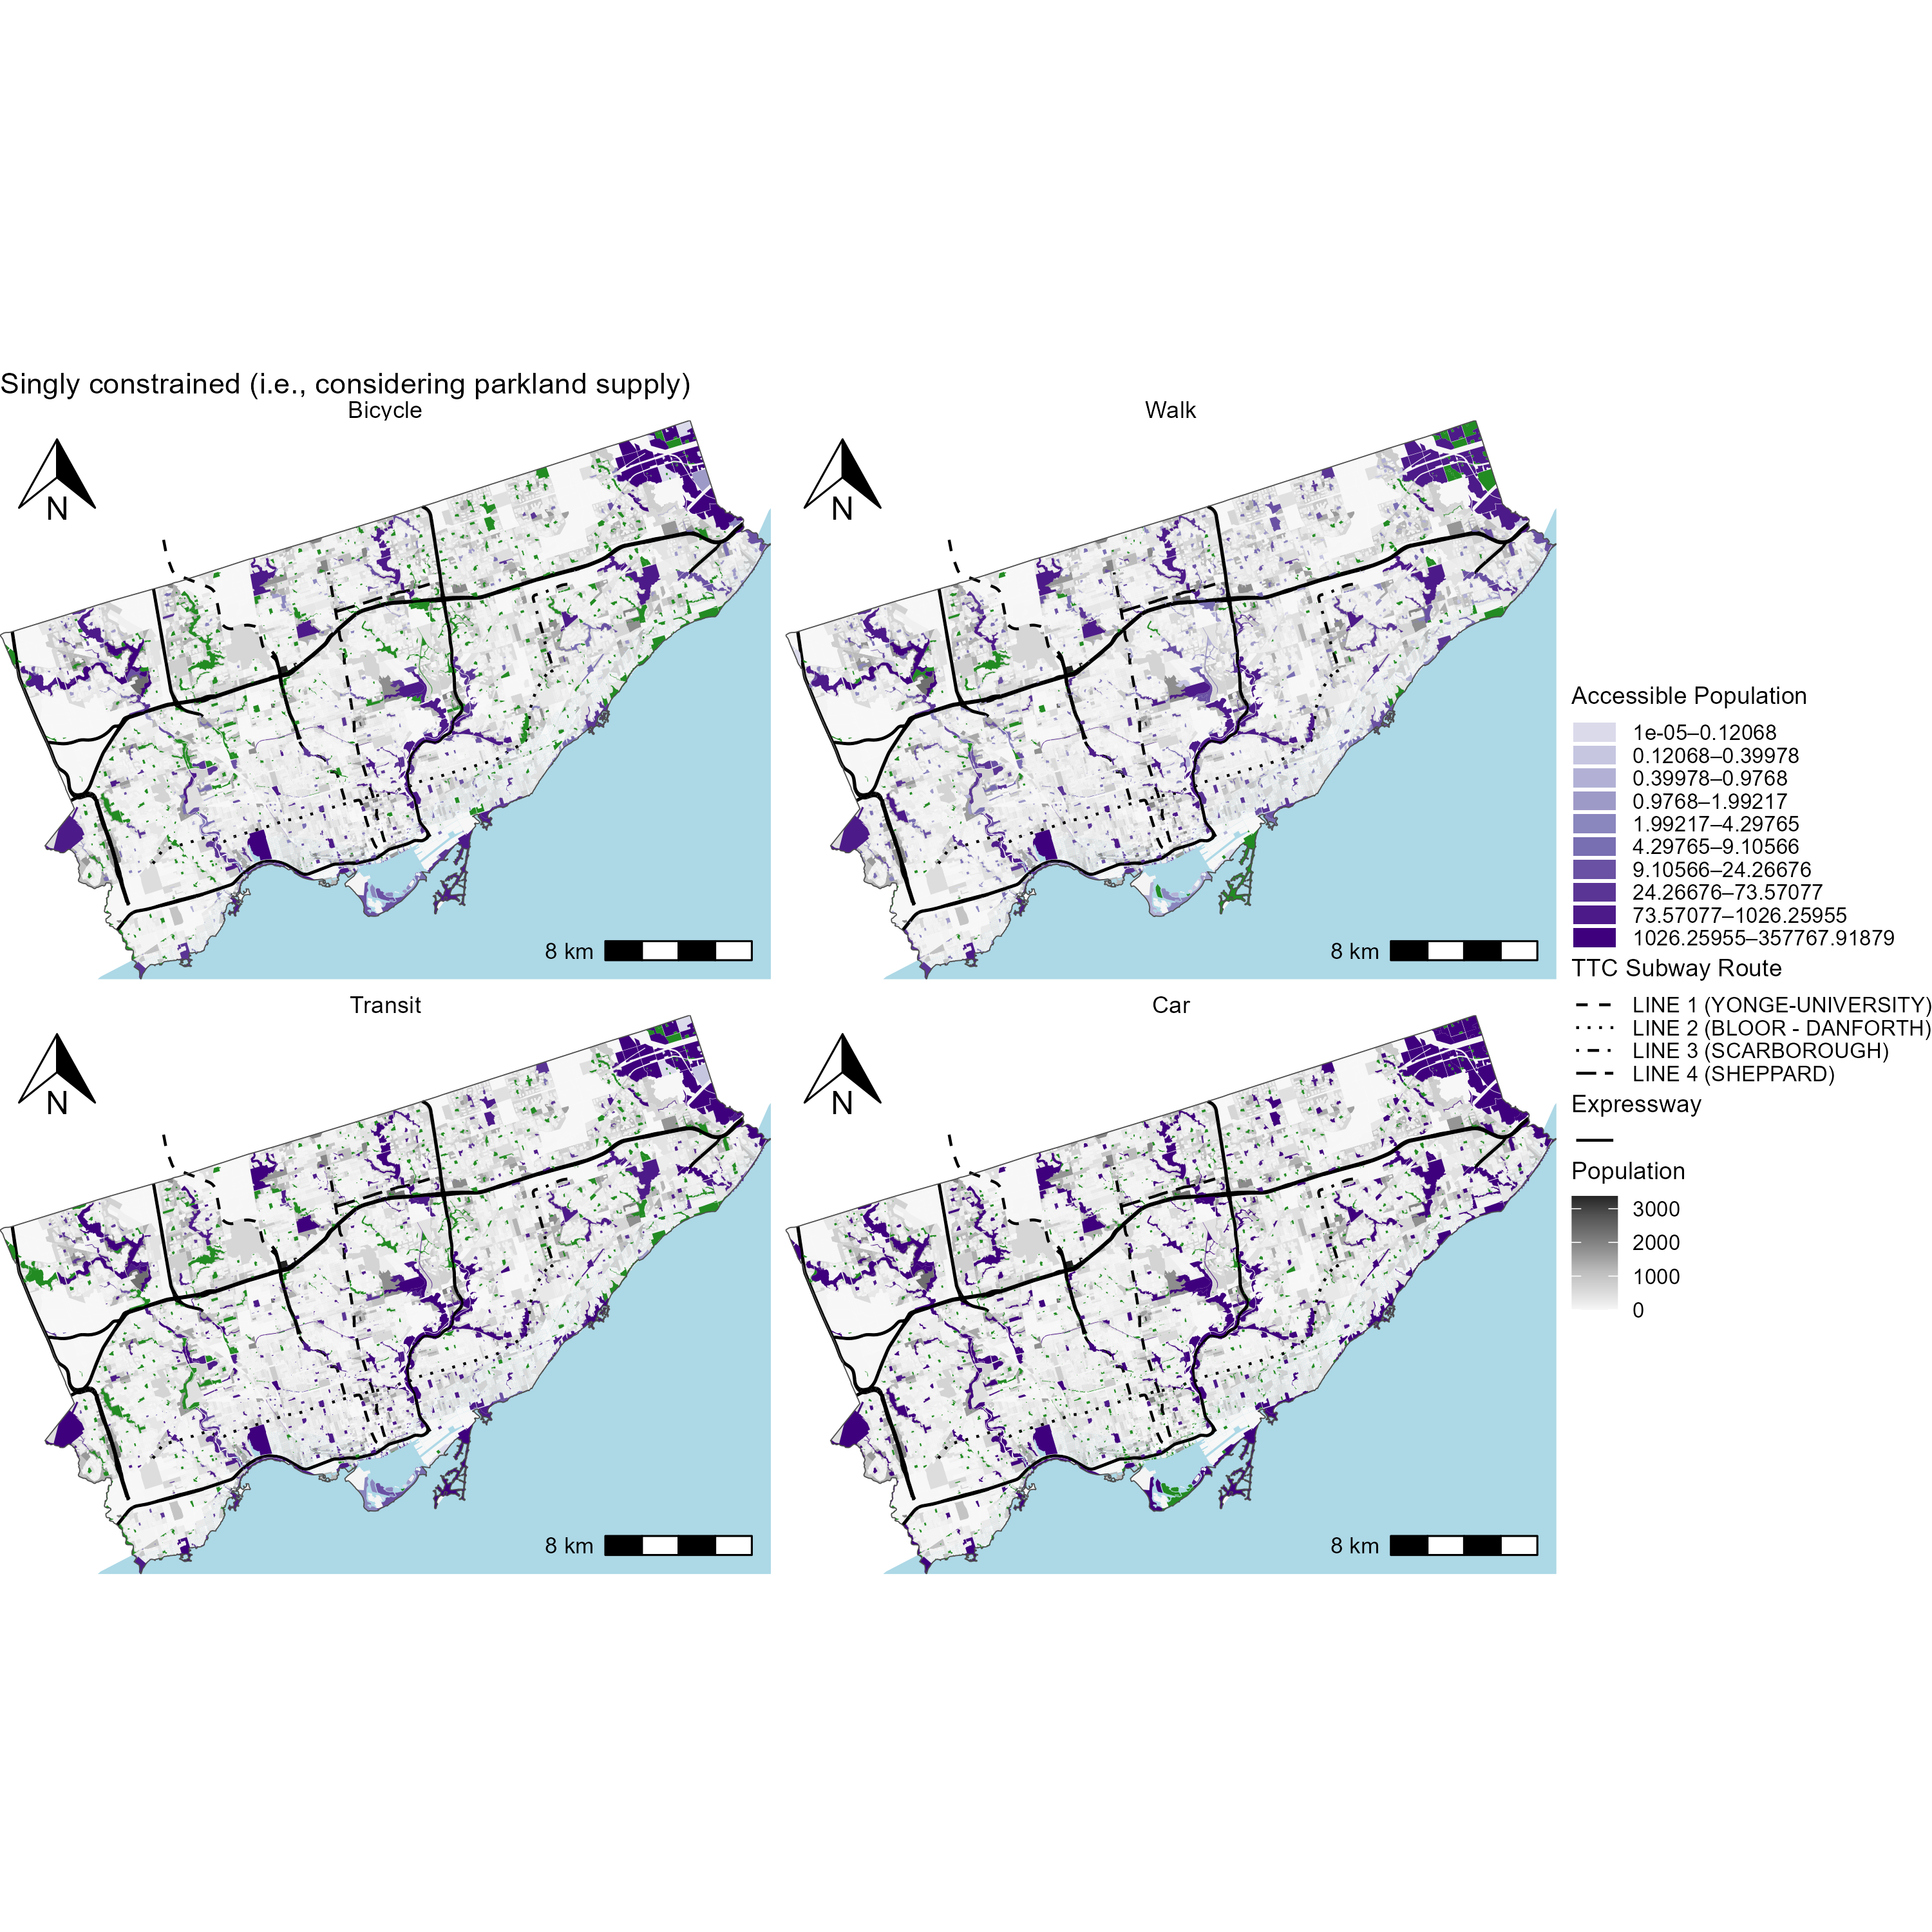
\includegraphics[width=6in]{./data/figures/chp5-pop_singly_access_parks_allmodes_plots} 

}

\caption{\label{fig:chp5-pop_singly_access_parks_allmodes_plots} Singly constrained multimodal accessible population by mode per park.}\label{fig:unnamed-chunk-88}
\end{figure}

In Figure \ref{fig:chp5-pop_singly_access_parks_allmodes_plots}, the singly constrained measure allocates the total population from each origin to the mode-specific parkland area supply which is a proportion of the incoming population. The result is the majority of multimodally accessible population (91\%) being allocated to the car-specific parkland supply. The remaining shares are allocated to transit-specific supply (8\%), cyclist-specific supply (1\%), and pedestrian-specific supply (1\%).

Why do these singly constrained results vary so wildly from the total constrained results? Due to the consideration of mode-specific parkland supply competition. Parks are visited predominately by cars--especially parks that have larger area and hence amount for a larger proportion of modal supply that is assumed to be car-specific. Furthermore, larger parks that have this larger amount of car-specific supply are outside the downtown core area, where car-mode share is higher. And again, car mode has the lowest travel impedance. Together, these factors work to allocate the vast amount of multimodally accessible population to car-specific supply.

The difference between total and singly constrained multimodally accessible population is more drastic than in the results of the preceding section. Why may this be? Due in part to the difference in origin and destination zoning systems and the impact of competition. Parks and DBs are in different zoning systems: where parks represent themselves and DBs represent a variable aggregation of the population with some uniformly throughout the city. Hence, as the total constrained measures only considers the mass of one zoning system (i.e., only the mass of the DBs in the case of multimodally accessible population), results between the \emph{accessible parkland area} and \emph{accessible population} are not directly comparable. However, under the singly constrained measure, both zoning systems are considered: the mass of the origins and the destinations, though only one is `constrained'. In this way, results are more stable. While the amount of `car-specific parkland supply' and `car-using population' are not in directly comparable units--the amount of accessibility that is allocated to a specific mode group (where it is origin-side or destination-side) can be intuitively compared.
\#\# Conclusions: comparing multimodal accessible parkland and accessible population by Toronto neighbourhood

This section summarises key patterns in multimodal constrained accessibility across Toronto neighbourhoods, focusing on two perspectives:

\begin{itemize}
\tightlist
\item
  Multimodally accessible parkland area: how total parkland is allocated based on origin-side modal split (representing mode-using population) and travel impedance (i.e., how much parkland area can be accessed from each DB each mode-using population group);
\item
  Multimodally accessible population: how total population is allocated to parks based on destination-side modal split (representing mode-specific parkland supply) and travel impedance (i.e., how many people can access each park by mode-specific parkland supply).
\end{itemize}

To contextualise the results, the previously discussed values are aggregated at a common scale: by Toronto's six former municipalities. Parks tend to align with these boundaries, and each area exhibits distinct spatial and infrastructural characteristics. Recall: Figure \ref{fig:chp3-mode_split_eachDB_plots} displays the boundaries of these former municipalities.

\subsection{\texorpdfstring{\textbf{How reachable is the parkland area to the population?}}{How reachable is the parkland area to the population?}}\label{how-reachable-is-the-parkland-area-to-the-population}

If asking this question, one is interested in evaluating the amount of accessible parkland area from all population-relevant locations across the city. If information about travel to parks by mode is lacking, one could use the \emph{multimodal total constrained opportunities measure}. In this approach, the total parkland area in the region is allocated to each origin zone solely based on travel impedance of each mode relative to all modes in the system. This measure reflects how much accessibility to parkland area a zone has for each type of modal population. The amount of population accessing the parkland area does not enter equation: faster modes can allocated a larger proportion of parkland area of the total, reducing the amount that other mode-users are allocated. The \emph{amount} of mode-using population at a location does not impact results. In this way, parkland area is treated as an inexhaustible resource.

However, if we do have information about parkland demand by modal group and we view parkland area as exhaustible, then a more refined question can be asked: \textbf{How much parkland area from each park is available to each modal-group of the population?}. In this case, the \emph{multimodal singly constrained opportunities measure} is appropriate. Here, accessibility is allocated competitively, considering both the spatial distribution of modal travel impedance (as in the total constrained measure) as well as the associated modal population (demand). These two dynamics are used to allocate only the parkland area available at each park to the mode-using population group at each origin.

Figure \ref{fig:chp5-mm_vv_T_S_muni_plots} summarises these two constrained measures across former Toronto municipalities, for the parkland area and population data used in this chapter on a per capita basis. Additionally, these plots visualise the amount of actual parkland area per area within the boundaries of each former municipality as well as the 12 sqm parkland area threshold.

\begin{figure}

{\centering 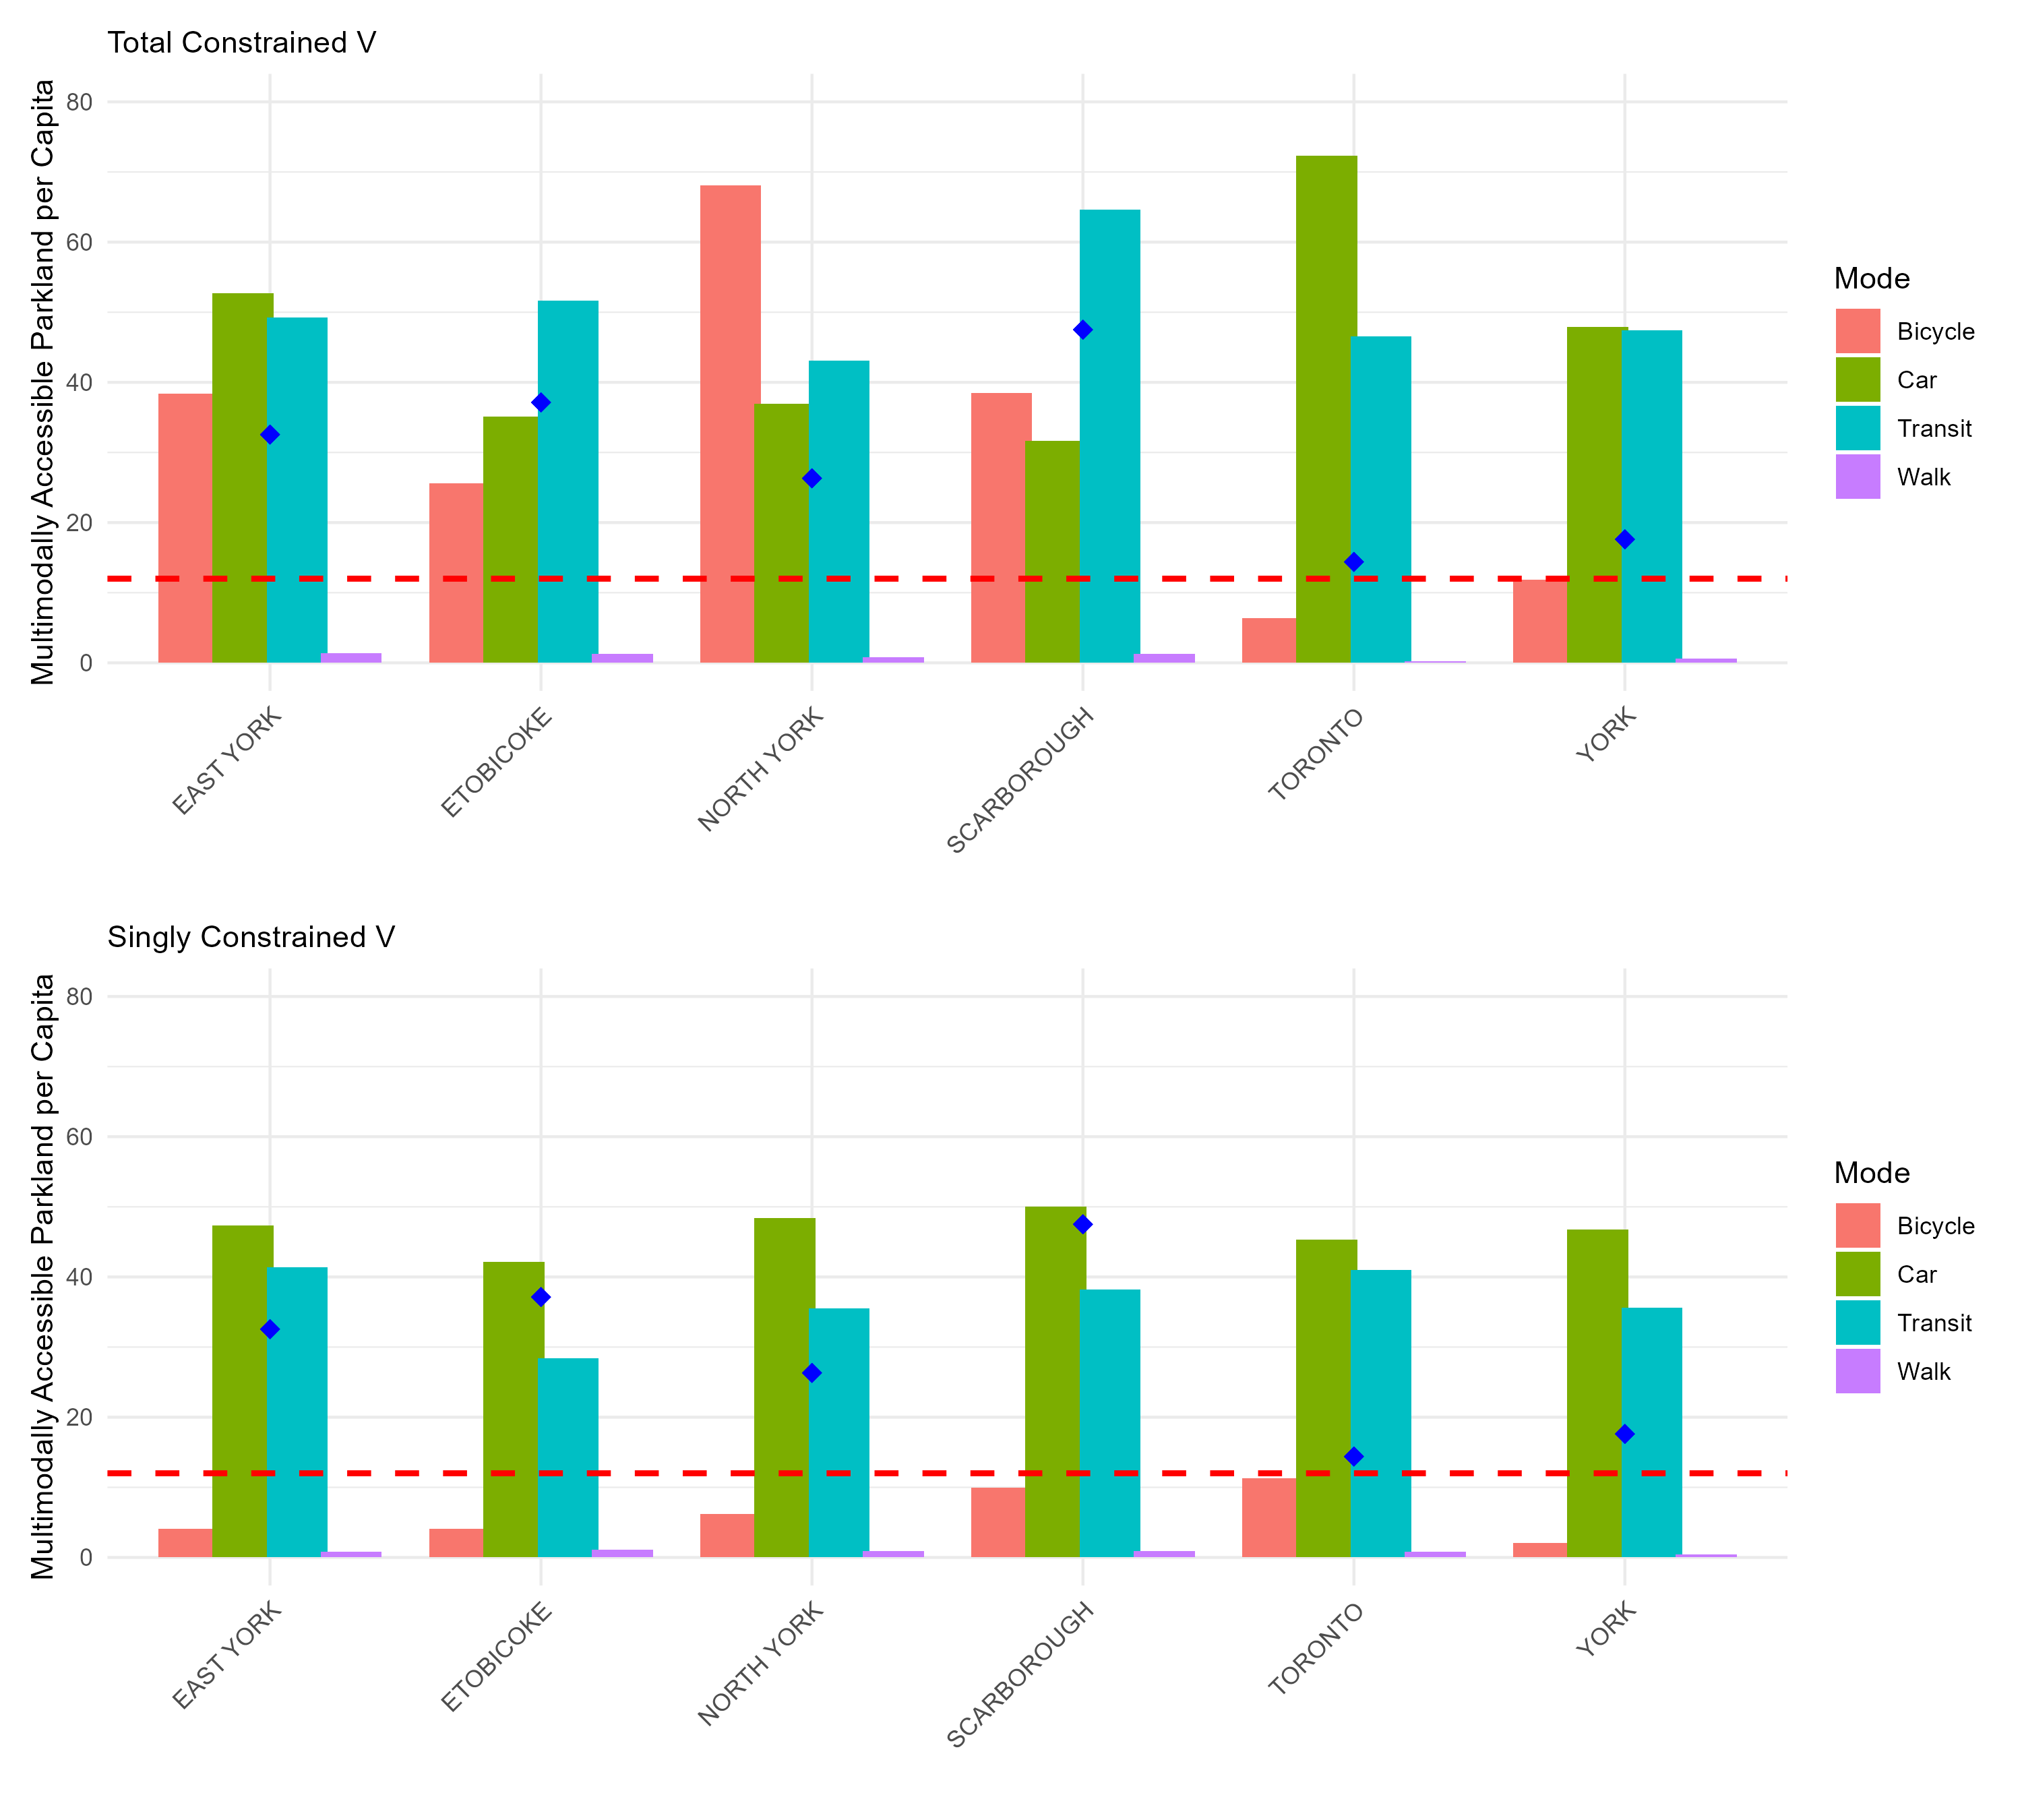
\includegraphics[width=6in]{./data/figures/chp5-mm_vv_T_S_muni_plots} 

}

\caption{\label{fig:chp5-mm_vv_T_S_muni_plots} Mutimodally accessible population summarised by former municipalities and plotted against real parkland area and population within the municipality. The diamond point represents the real amount of parkland area per capita in the muncipality and the dashed red line the 12 sqm per capita threshold.}\label{fig:unnamed-chunk-89}
\end{figure}

The multimodally accessible parkland per capita is consistently below the 12 sqm threshold for walking populations in all former municipalities. This is due to the inherently high travel impedance of walking (limited to a 15-minute radius). Even in former municipalities with dense and centrally located walking populations, like Toronto, only those directly adjacent to parks see higher levels of access (e.g., as discussed concerning Figure \ref{fig:chp5-mm_parkland_concs_access_DB_plots} and Figure \ref{fig:chp5-mm_parkland_singly_conc_access_DB_plots}). The assumed walking populations fall short in capturing plenty of parkland area, as their travel `reach' is uncompetitive compared to other modes.

In contrast, motorised modes consistently exceed the 12 sqm per capita threshold and yield the highest levels of multimodal accessible parkland area. This is expected, given their lower travel impedance, which allows populations to access parks well beyond their local boundaries unlike non-motorised modes with higher travel impedances that only assume they reach a handful of proximate parks. Notably, under the total constrained measure, transit accessibility often exceeds car multimodal accessibility in more suburban municipalities like Etobicoke and Scarborough. This suggests that, on a per mode-user basis, transit is a more competitive mode for park area accessibility when only relative modal reachability of parks and their amount of parkland area is considered.

However, the total constrained measure does not capture the full picture. When modal population is accounted for within the measure itself (the singly constrained measure), across the city transit-users are allocated lower amounts of accessible parkland area while motorists receive consistently the highest amount. Why? As mentioned, the motorist population is much higher in these suburbs, but also present in high numbers across the city. Even in most urban Toronto municipality--where transit infrastructure is dense and well connected to parks--the car mode still maintains an edge in per capita parkland accessibility (though the edge is smallest for this municipality), underscoring the impact of considering modal competition in the accessibility results. Indeed, we may see the competitive advantage of the mode's connectivity to the amount of opportunities with the total constrained measure, but in also including the amount of mode-users that use the mode (the singly constrained measure), it is clear that still the car mode is most competitive on a per capita basis at capturing multimodally parkland area.

Cycling values also present a more nuanced story, as their ratios are less stable across neighbourhoods and between the two measures. When modal population competition is not considered, cycling tends to show high per capita multimodal accessibility in municipalities with lower modal bike share i.e., everywhere except York and Toronto. But once population demand is introduced, cycling per capita rates fall below the 12 sqm threshold in all municipalities. The reason, again, is relative modal population competitive: car users, with lower impedance and higher population amounts, capture more shares of the multimodally accessible parkland area. The \emph{amount} of other mode-users capturing accessible parkland area drive the difference in ratio in the difference between teh total and singly constrained ratios. This is interesting, because it suggests that these areas are very well connected to multimodally accessible parkland area by cycling on a per cyclist capita, but when the amount of cyclists is considered in the measure itself, the ratio drops, just like in the case of transit.

For cycling, like in the case of transit as well, per capita singly constrained measure produces less variability across neighbourhoods than the per capita total constrained measure. This is because it responds directly to mode-specific population distribution. Across all municipalities, active modes (walking and cycling) remain below the threshold, while car access consistently outperforms all others followed by transit, cycling and then by foot. But still, the impact that spatial centrally has on allocation in the singly constrained measure is present: the more densely populated and centrally located municipalities of Toronto and York have much higher per capita accessible parkland area (particularly by motorised modes) than the amount of actual parkland area within their boundaries.

If the goal is to improve multimodal park accessibility for non-car modes, several insights emerge from these per capita results. In suburban municipalities with strong cycling connectivity but low bike usage, soft infrastructure--such as signage, safety improvements, and promotion of existing routes--can support a shift toward cycling. At the same time, reducing car's accessibility through hard infrastructure changes (e.g., restrictions on speed, on routes) or through soft infrastructure (e.g., by limiting park parking) and enhancing transit options (e.g., through dedicated shuttles or targeted routes) can help redirect demand away from driving which shifts mode-split and increases multimodally accessible parkland area for non-car modes. Finally, mode-specific accessibility thresholds should be considered, as a uniform target (e.g., 12 sqm per capita) may not suit all modes. For instance, lower sqm per capita thresholds for active modes and higher ones for transit may better reflect what equitable, mode-sensitive accessibility could look like. This should be a topic for further investigation.

\subsection{\texorpdfstring{\textbf{How reachable is the population from parks?}}{How reachable is the population from parks?}}\label{how-reachable-is-the-population-from-parks}

If evaluating how efficiently the park provides multimodal accessibility to population but the amount of mode-suitable parkland area supply for the parks is unknown: one can choose the \emph{total constrained accessible population measure}. Using this measure, the total population is allocated to each park based only on the modal-group's travel impedance. With this measure, one can understand how much population by modal group is within reach of each park and can be aggregated at different levels to reflect this amount.

However, if one does have information about modal parkland supply and we view population at each origin as exhaustible, then we can ask a more refined question: \textbf{How much population from each origin is multimodally accessible to each park?} In this case, the \emph{multimodal singly constrained population measure} is appropriate. Here, accessible population is allocated competitively, considering both the spatial distribution of modal travel impedance (as in the total constrained measure) as well as the associated mode-specific parkland area (mode-specific supply) to allocate the population available at each DB to the mode-specific parkland supply at each park.

Figure \ref{fig:chp5-mm_vv_T_S_muni_plots} summarises these two constrained measures across the former Toronto municipalities on a per parkland hectre basis. As well, these plots visualise the amount of actual population per hectare of parkland within the boundaries of each former municipality (represented by black trianges). Additionally, note the different ranges in the horizontal scale for the two measures. Though a population per parkland area threshold is not visualised, for reference, the inverse of the 12 sqm parkland area per capita threshold is 833 people per parkland hectare. So, if a municipality represents parks with a ratio of 10 people per walk-specific parkland hectare and 1000 people per transit-specific parkland hectare, this means that population is 10 times more reachable to parks by transit than by foot.

\begin{figure}

{\centering 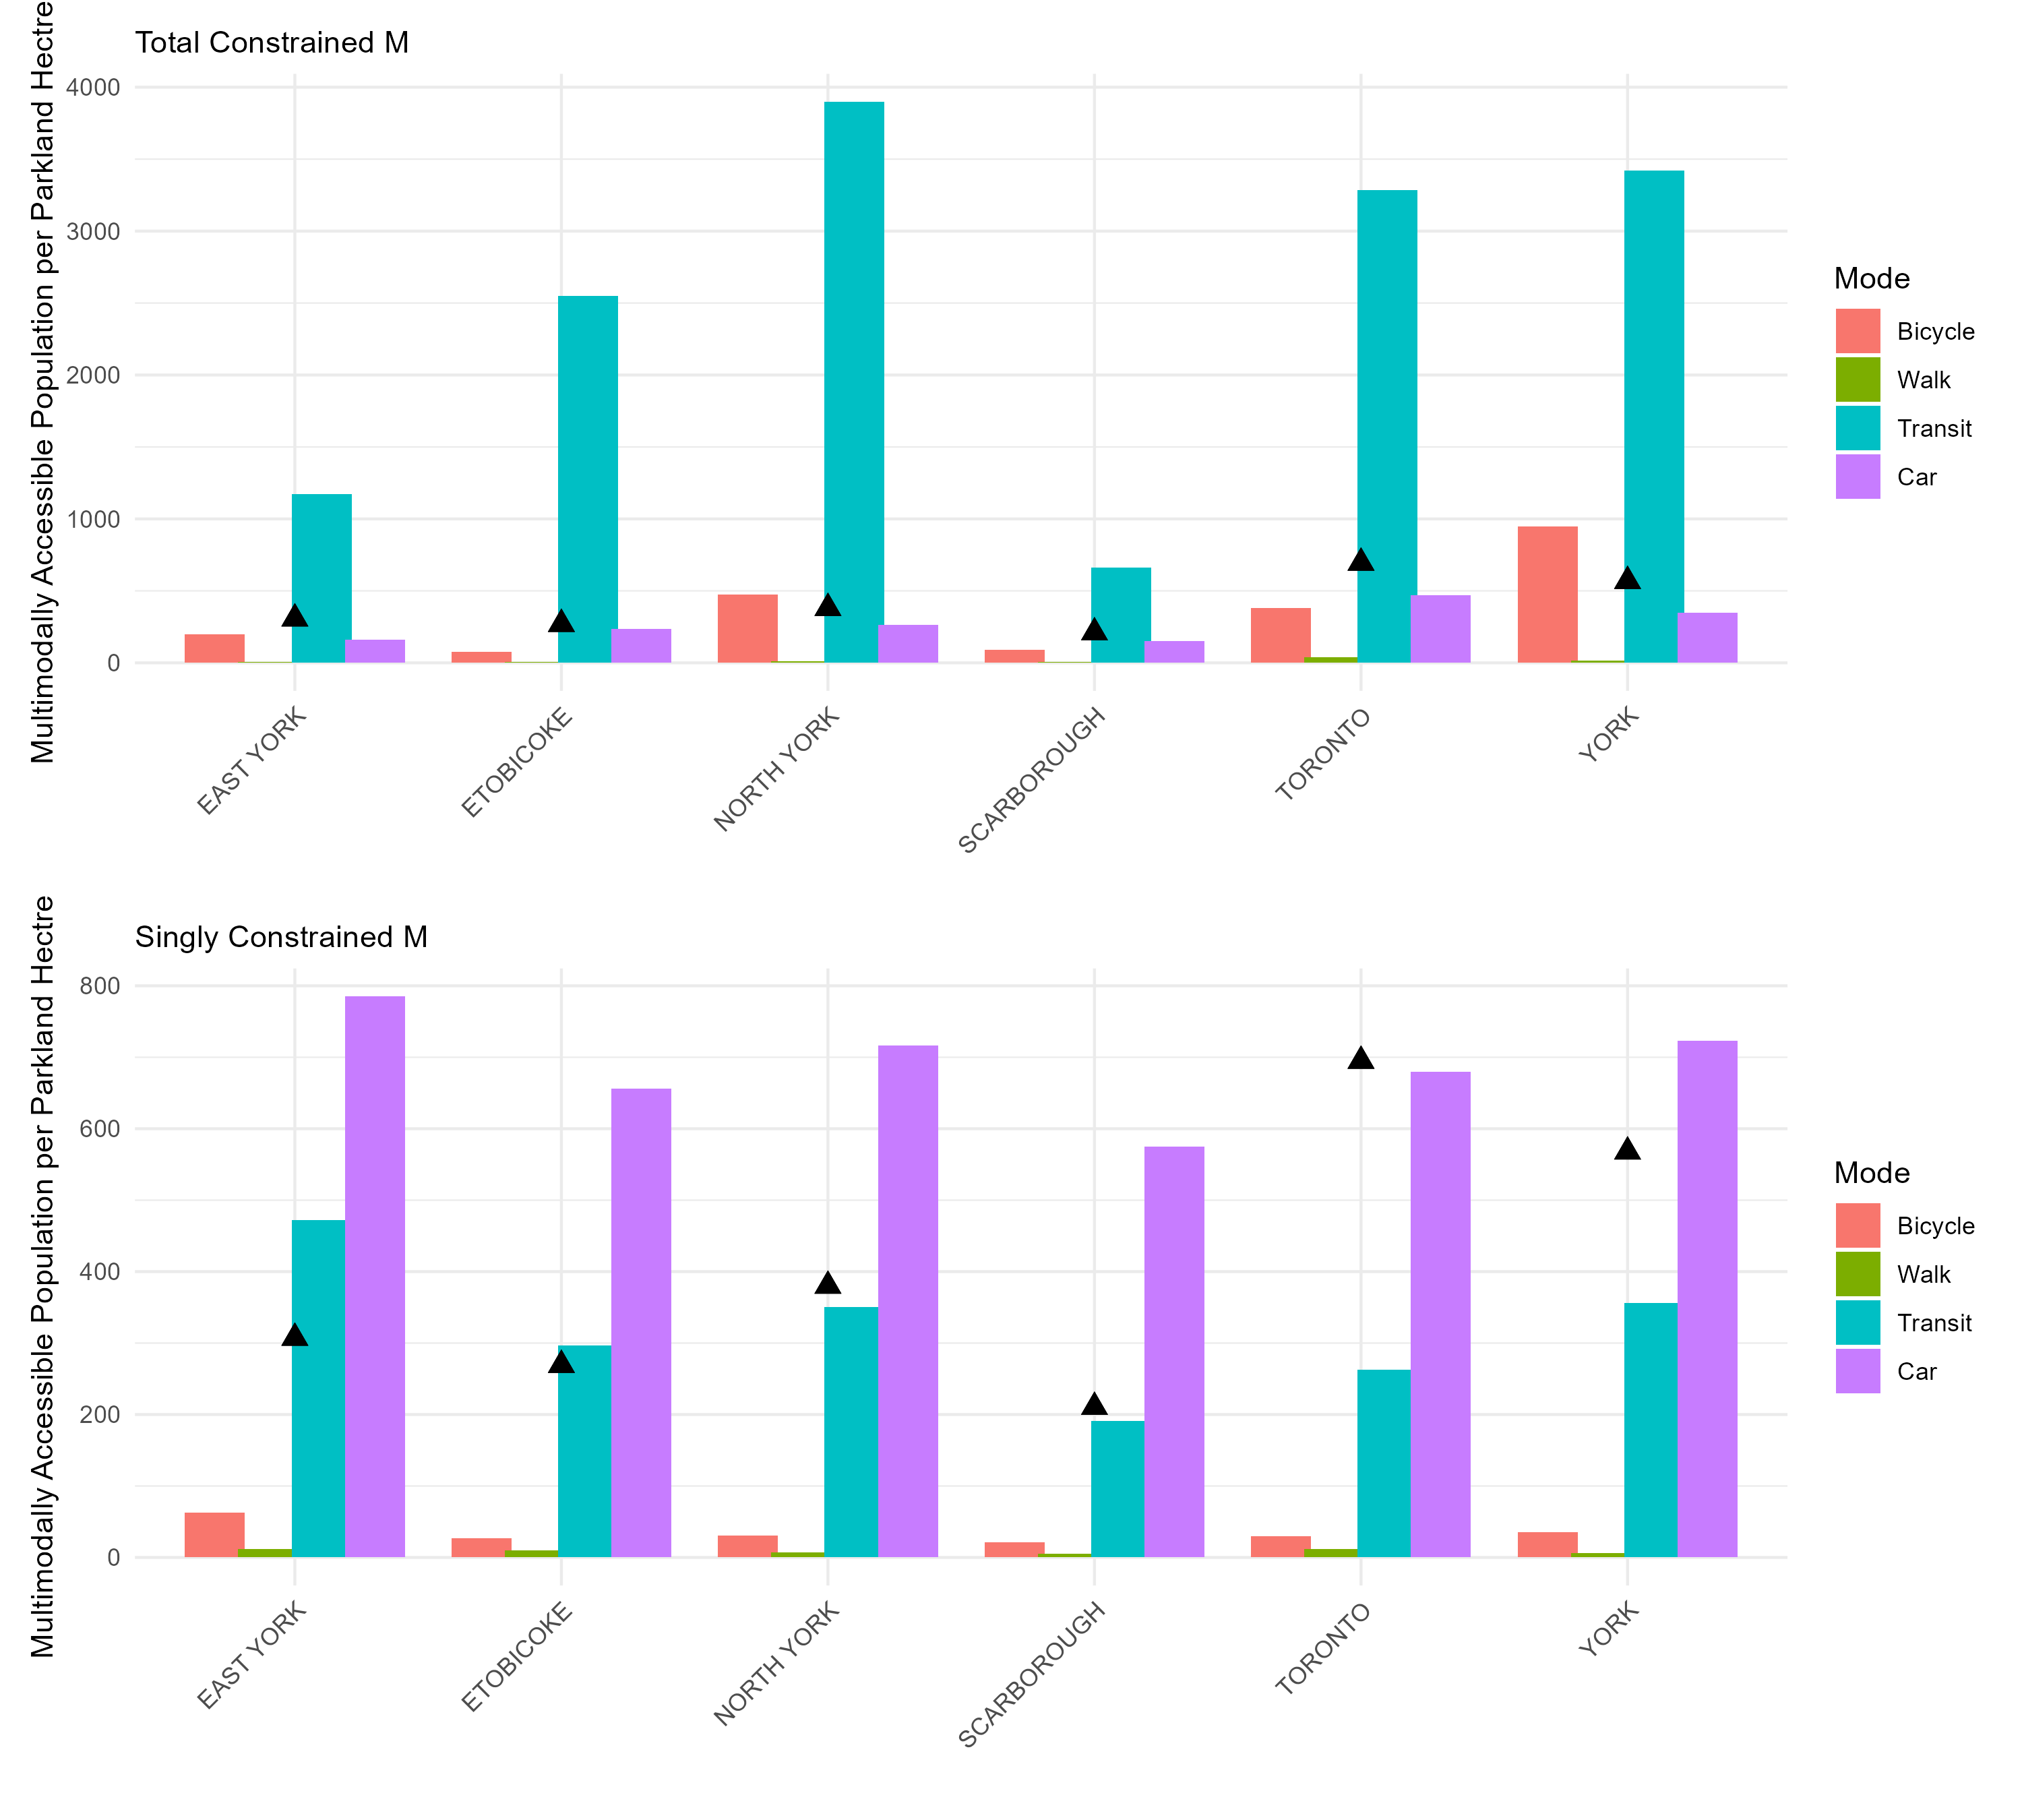
\includegraphics[width=6in]{./data/figures/chp5-mm_mm_T_S_muni_plots} 

}

\caption{\label{fig:chp5-mm_vv_T_S_muni_plots} Mutimodally accessible population summarised by former municipalities and plotted against real parkland area and population within the municipality. The triange point represents the real amount of population per parkland area (person per hectare) in the muncipality.}\label{fig:unnamed-chunk-91}
\end{figure}

Across both measures, one consistent pattern emerges: walking accessibility per hectare of walk-specific parkland is low citywide, regardless of whether mode-specific supply is considered within the measure. As mentioned: this is due to the assumed limited 15-minute range of walking which results in only the populations in immediate proximity to a park being allocated the mode-specific supply. Although walking is the second most common mode for park visits (see Figure \ref{fig:chp3-mode_split_parks_plots}) so its assumed walk-specific parkland supply is relatively high, it still cannot overcome its short spatial reach. As a result, only a relatively small amount of walking-population is allocated per walking-accessible hectare relative to the other modes that can be matched to mode-specific supply by DBs much further away.

Otherwise: modal rates by the total and singly constrained measures are quite different. Focusing on the difference between car and transit values, introducing mode-specific parkland supply into the measure has a dramatic effect on per capita ratios. For transit, the shift is especially noticeable: under the total constrained measure 800 transit-using people per transit-specific parkland hectare and above is the ratio whereas these ratios drops to below 700 across the city when considering the singly constrained measure. This drop is attributed to two related factors: first, car-specific parkland supply is quite high, particularly at the larger parks that make up the majority of the city's total parkland area. In this way, when considering the singly constrained measure, this large supply demands a large amount of the reachable population. Second, while transit may be more competitive in \emph{reaching} people from parks under the chosen assumptions (e.g., its travel cost function and how it can access all parks), when mode-specific supply is considered, this cost effect is surpassed by the impact of car's (and other modes')-specific parkland area supply's competitive advantage is attracting population. In other words, even though transit connects well to parks, the relatively lower spatially distributed amounts of transit-specific parkland, shifts much of the `total constrained' multimodally accessible population from transit to car.

Cycling exhibits a similar pattern as transit, in how its ratio decreases when competitive mode-specific supply is considered. Although the cycling network can connect many people to parks (high total constrained ratios), parks with high multimodally accessible population by bike-specific supply tend to be smaller in size--as car is assumed not to reach them--and are the same parks highly reachable by non-car modes. So when mode-specific supply competition is factored in, population is competed for by this non-car-specific supply, and car-specific supply is especially advantaged as it is plentiful in parks that are not as well connected by all the other modes \emph{as well} as having the lowest travel imepdance.

The diamond points in Figure \ref{fig:chp5-mm_vv_T_S_muni_plots} represent the static population-to-parkland hectare ratios within each municipality. The accessibility ratios for far-population-reaching modes, like transit under the total constrained measure, often exceed these static ratios--demonstratining transit's strong potential to connect people from within and beyond the boundaries of the municipality to parks within its boundaries. And as discussed, under the singly constrained measure, transit's competitive advantage relatively shrinks reflecting a mismatch between the transit network's high levels of connection of people to parkland area and the actual transit-specific park supply (i.e., amount of transit-using visitors to parks weighted by parkland area). Encouraging more people to use transit to reach parks--particularly in place of car trips--would result in more balanced transit and car singly constrained ratios, ratio thresholds that could be formulated into a planning target.

From the opposite perspective, low accessible population per mode-specific hectare ratios may also not be advisable as they signal inefficient mode-specific supply reachability. Just as the 12 sqm per capita threshold is used to assess park equity, a mode-specific population-per-hectare threshold could offer a complementary benchmark to the underlying intuition. These multimodal accessible population thresholds would capture how efficiently parks serve different travel mode populations, and could be calibrated to align with broader goals of promoting wellbeing, social interaction, and community connection, i.e., each hectare of park should aim to be accessible to X amount of people by motorised modes and Y amount of people by active modes. As with the multimodal accessible parkland area thresholds, this is a topic for further investigation.

\chapter*{Conclusion}\label{conclusion-1}
\addcontentsline{toc}{chapter}{Conclusion}

\section{Dissertation Summary}\label{dissertation-summary}

Though accessibility can be defined in many ways, most trace back to Hansen (1959): ``the potential of opportunities for interaction\ldots{}'' (p.~73). Yet within this definition, a key question remains unresolved: does accessibility have units? One could argue, as this dissertation does, that accessibility should be in the units of \emph{opportunities} that are up for potential spatially interaction. In current practice, however, accessibility is often treated as unitless, which undermines clarity and comparability. To address this, this dissertation develops a detailed motivation, proposes a methodological framework that restores units via a `family of accessibility measures', and uses a Toronto-based case study to demonstrate how the absence of defined units limits interpretability and descriptive analysis.

More specifically, this dissertation offers a novel approach to the accessibility literature by adopting balancing factors from spatial interaction modelling literature into the accessibility context. These balancing factors keep accessibility results comparable to conventional accessibility measurement methods but ensure values retain meaningful units--units tied to tangible system characteristics, such as the total number of opportunities in a region or the known number at a specific destination. The contributions of this dissertation are four-fold:

\begin{itemize}
\tightlist
\item
  First, it explicitly links accessibility to spatial interaction through their shared intellectual foundations (pre- Hansen (1959)), highlighting how contemporary accessibility research has diverged and showing the mathematical, intuitive, and interpretative advantages of preserving units through constrained formulations, as done in spatial interaction modeling.
\item
  Second, it introduces the total constrained accessibility measure as an alternative to the Hansen-type formulation, producing zonal values that represent proportions of the known number of destination masses (i.e., opportunities) or origin masses (i.e., population) in the region.
\item
  Third, it presents the singly constrained accessibility measure as a competitive method that proportionally allocates opportunities from the destination based on population demand (from the origin), or in the case of market potential, proportional allocation of population from the origin based on the supply of opportunities at the destination. Its per-capita zonal rate is shown to be mathematically equivalent to the widely used two-step floating catchment area (2SFCA) method (Luo \& Wang, 2003; Q. Shen, 1998).
\item
  Fourth, responding to the scarcity of coherent multimodal accessibility frameworks in the literature, this work extends both the total- and singly-constrained accessibility measures to account for multiple modes of transportation.
\end{itemize}

The \textbf{first contribution} of this dissertation, presented in Chapter 1, revisits the widely cited definition of accessibility from Hansen (1959): ``the potential of opportunities for interaction\ldots{} a generalization of the population-over-distance relationship or population potential concept developed by Stewart (1948)'' (p.~73). This work traces this definition back to its Newtonian roots in human spatial interaction modeling, beginning with Ravenstein (1885), and investigates how the units of ``the potential of opportunities for interaction'' were originally defined. This probing review leads to the family of spatial interaction models developed by Wilson (1971), particularly his introduction of balancing factors designed to reflect known system constraints--such as the total constraint, and the production and attraction constraints (represented in Equations \ref{eq:constraint0-gravitymodel}, \ref{eq:constraint1-gravitymodel}, and \ref{eq:constraint2-gravitymodel}). Notably, while these models formalized interaction mechanisms using system constraints, the concept of accessibility itself was not explicitly or meaningfully developed within.

Having established that spatial interaction and accessibility share common roots, the chapter next examines how these two bodies of literature have interacted in the contemporary era. It reviews works that cite both Hansen (1959) and Wilson (1971) and reveals that, despite their shared origins, accessibility and spatial interaction modeling literatures have largely remained distinct. One stream of the literature is more focused on spatial interaction modeling and cites Hansen (1959) as the father of the accessibility concept and/or uses accessibility as a variable (or additional variable) within the spatial interaction model itself. In these cases, accessibility is treated as conceptually related to spatial interaction, but the connection is not clearly or practically clarified. Another body of work is more accessibility-focused and is mostly part of the contemporary accessibility literature which gained momentum in the early 2000s. These accessibility-focused works cite Wilson (1971) for a variety of general reasons, but none (other than Soukhov et al. (2023) and Soukhov et al. (2024)) cite the rationale of Wilson's constraints.

Beginning with this rationale in Chapter 2, the balancing factors, akin to those used in Wilson's family of spatial interaction models, are introduced in the context of accessibility. The chapter details the interpretive advantages of these factors, particularly their ability to produce accessibility values with meaningful units (e.g., a share of opportunities in the region) while incorporating system-wide or zonal constraints based on known quantities. Overall, Chapter 2 presents a `family of accessibility measures', constructed using the constrained intuition of Wilson's spatial interaction models, and illustrated through a simple toy example. Alongside the conventional formulation of accessibility as the potential of opportunities for spatial interaction--or simply, ``accessible opportunities'' from a zone--Chapter 2 also defines its transpose: the potential of population for interaction or `market potential'.

This dissertation is among the first to investigate the relationship between spatial interaction modeling and accessibility measures in the contemporary era, which is its \textbf{first contribution}. This dissertation applies the constraining mechanism of balancing factors--not only to the measurement of accessible opportunities, but also to accessible population (i.e., market potential). This introduces a methodology to the accessibility literature that produces unprocessed accessibility outputs that can be directly interpreted in units of opportunities (or population) for potential spatial interaction at a zone.

The \textbf{second contribution} of this dissertation is the introduction of the total constraint to accessibility measurement. The total constrained measure is conceptually equivalent in magnitude to the Hansen-type accessibility measure (Equation \ref{eq:access-unconstrained}) but is expressed in meaningful units--the number of accessible opportunities at a given zone, or accessible population in the case of market potential. As such, the total constrained measure remains compatible with the commonly used Hansen-type measure (or unconstrained, as referred to in this work), while offering improved interpretability of the resulting raw values.

The total constrained accessibility's formulation is presented in Chapter 2, and an empirical example focused on accessible parks in terms of parkland area and population is detailed in Chapter 3 (data and methods) and Chapter 4 (results) with a unimodal example, only considering accessibility by walking. In these empirical results, the total parkland area in the region is proportionally allocated to each origin zone through the total constrained proportionality factor that ensures it remains proportion to the unconstrained measure. However, unlike unconstrained measures, the resulting values are expressed in known, interpretable units. This leads to several practical and promising advantages: the values can be intuitively understood, aggregated across different spatial scales (e.g., neighbourhoods with varying equity classifications), and expressed on a per capita basis. This per capita framing enables direct comparison against policy-relevant benchmarks, such as Toronto's standard of 12 sqm of parkland per person (City of Toronto, 2019).

Without units tied to tangible system quantities--such as total parkland area or total population--such comparisons would be far less clear. This interpretability makes the approach especially promising for applied researchers and practitioners seeking to inform equitable planning and policy decisions.

This dissertation's \textbf{third contribution} is the introduction of the singly constrained accessibility measure, formulated in Chapter 2 and 3, and applied alongside the unconstrained and total constrained accessibility measures in Chapter 4 focusing on accessible parkland area (from origins) and accessible population (to parks) in a unimodal, walking-only context.

The singly constrained measure applies a single constraint--either at the destination (opportunity side) or the origin (population side)--ensuring that the total amount of opportunities or population is preserved and proportionally allocated. In doing so, it implicitly satisfies the total constraint. For example, when parkland area (opportunities) are constrained, they are proportionally allocated to each origin zone based on relative accessibility, while ensuring that the total amount of parkland area allocated from each park matches the actual total regional supply of parkland area. This captures competition for opportunities across zones, an aspect that is not considered in the total constrained accessibility measure.

Put another way, the singly constrained measure (in the case of accessible opportunities) accounts for the exhaustibility of opportunities. While the total constrained approach distributes the regional total based on travel impedance-weighted accessibility, it may over- or under-allocate individual parkland area. For example, parks that tend to be over-allocated are larger and in more central and reachable areas; so these parks end up contributing more accessible area relative to the area they physically have. This relative over-allocation is an indicator that, spatially the park is centrally located and could be facing issues of population congestion. In contrast, the singly constrained measure ensures that each park's contribution is limited to its actual size, allocated proportionally among populations based on both proximity and demand, effectively folding in this concept of `population congestion' within the measure itself. This leads to a more sensitive accessibility that accounts for population competition, i.e., large parks that are centrally located can still be highly accessible, but competition from surrounding populations moderates the accessible parkland area that is proportionally allocated.

The per capita variant of the singly constrained measure is mathematically equivalent to the popular Two-Step Floating Catchment Area (2SFCA) method (Luo \& Wang, 2003), so it too fits neatly within the accessibility literature. Like the total constrained measure, the singly constrained measure allows for intuitive aggregation at larger spatial units (e.g., neighbourhoods) and supports comparisons with politically relevant benchmarks, such as Toronto's parkland supply threshold (e.g., 12 sqm per capita in City of Toronto (2019)).

By measuring accessibility under the assumption that opportunities (or population, in the case of market potential) are exhaustible, the singly constrained measure offers a practical and interpretable framework for applied researchers and practitioners. It enables analysts to incorporate information about both origin and destination ``marginals''--even when the specific interaction between them is not known. This makes the singly constrained accessibility measure particularly well-suited for applications where understanding localized competition for exhaustible resources (like park space) is important.

The \textbf{fourth contribution} of this dissertation is the multimodal extension of both the total- and singly-constrained accessibility measures. This development responds to a notable gap in the accessibility literature, where coherent approaches to multimodal accessibility remain underdeveloped. By extending the measure to incorporate multiple transportation modes (walk, bicycle, transit, and car) with different travel characteristics and corresponding mode-using groups at the origin or mode-specific groups at the destination, this extension broadens the applicability of constrained accessibility and sharpens its intuitive value.

Like in the unimodal contributions: Chapter 2 presents the formal multimodal extensions for both accessible opportunities and accessible population (market potential), Chapter 3 outlines the relevant empirical data, including mode-specific travel impedance functions and mode-using populations and park-side mode-using proportions, and Chapter 4 details the empirical multimodal accessibility results.

In the case of accessible parkland area, multimodal accessibility to parkland area for each DB in Toronto is reported, as well as an expression of the amount of multimodal accessibility by a specific mode-using group for each zone. In this way, differences between the potential for spatial interaction with parkland area between certain mode-using groups (e.g., walking vs.~car) is possible within the same framework. For instance, plots that quantify how much more parkland area is accessible by car than walk is quantified, and can be done for other any relevant spatial unit. Additionally, this multimodal extension is explored in the case of multimodal accessible population for each park.

Together, these \textbf{four novel contributions} advance the field of accessibility analysis--methodologically, empirically, and interpretatively by:

\begin{itemize}
\tightlist
\item
  Linking accessibility and spatial interaction modeling through shared theoretical foundations and the use of balancing factors.
\item
  Introducing the total constrained accessibility measure, which offers unit-consistent, interpretable results aligned with real-world quantities without the need for information other than travel impedance values and spatial distribution of opportunities in the case of \emph{accessible opportunities} or spatial distribution of population in the case of \emph{accessible population}.
\item
  Detailing the singly constrained measure, which incorporates competition and resource exhaustibility (i.e., either opportunity-side single constraint or population-side singly constraint), offering a richer understanding of competitive accessibility.
\item
  Extending both constrained measures into multimodal variants, allowing meaningful comparisons between groups with different travel behaviours within the same framework.
\end{itemize}

In sum, the constrained accessibility measures developed in this dissertation provide a clearer conceptual and practical bridge between accessibility analysis and spatial interaction modeling. By working in units of accessible opportunities (or population), these constrained methods make results more interpretable, easier to communicate, and directly comparable to known thresholds (e.g., per capita parkland supply standards). The multimodal extension further reveals how high-accessibility groups (e.g., those using faster or more flexible modes) effectively draw access away from others, illustrating competition within shared urban systems.

Because the resulting values maintain consistent units, they can be meaningfully compared across zones, spatial scales, and over time. These methods can address long-standing challenges in accessibility research: the lack of comparability due to inconsistently defined or unitless measures.

The constrained accessibility measures introduced here offer methods that are not only theoretically grounded but also interpretable and relatively straightforward. Their flexibility allows them to be expressed per capita or per any zonal attribute, facilitating application across a wide range of policy contexts--from infrastructure planning to social equity assessments. By making accessibility more intuitive and grounded in tangible system metrics, this work aims to support urban planners and policymakers in designing fairer and more opportunity-rich cities.

\section{Future research directions}\label{future-research-directions}

The research presented in this dissertation can be expanded along a variety of directions. The following four are detailed:

\begin{itemize}
\tightlist
\item
  Robustness and comparability of accessibility analysis across scenarios, including varying temporal and spatial contexts;
\item
  The investigation of ``potential'' in accessibility;
\item
  Multimodal, multipopulation and multiopportunity accessibility analysis that is sensitive to digital opportunities and vulnerable populations; and
\item
  Enhanced planning for equitable and sustainable cities.
\end{itemize}

The \textbf{first} promising direction for future research is examining how constrained accessibility measures can enhance the robustness and comparability of results across scenarios. In particular, these measure may help improve comparability across different temporal and spatial contexts--either within the same region or between different regions--related to the Modifiable Areal Unit Problem (MAUP) and the Modifiable Temporal Unit Problem (MTUP). As noted in existing literature (Horner \& Murray, 2004; Tan \& Samsudin, 2017), results from spatial analyses are often sensitive to how data are aggregated, both in terms of scale (e.g., the level of spatial resolution, where larger zones may smooth over important local variation) and zoning configuration (i.e., how boundaries are configurated at a given scale). Similarly, temporal aggregations--such as travel time assumptions or peak-period averaging--can also yield different results and potentially quite conclusions (R. H. Pereira, 2019).

The constrained accessibility measures introduced in this dissertation are designed to express each zonal value as a proportion of a known regional total. This proportional allocation mechanism, by design, enables more consistent and interpretable comparisons, as all zones are evaluated relative to the same regional context. Analysts can select the unit of spatial and temporal analysis based on methodological suitability rather than an ad-hoc manner or driven by interpretability. Analysts can also test the sensitivity of their constrained results to changes in zoning or time intervals.

Moreover, the flexibility of the constrained framework allows analysts to adopt more behaviourally realistic models--such as using an exponential decay function for travel impedance instead of a binary threshold--while maintaining clear and communicable outputs. These enhancements not only support more nuanced methodological choices but may also lead to more valid and policy-relevant insights by better reflecting real-world travel behaviour. Ultimately, using a constrained framework creates more space for methodological complexity and coherent sensitivity testing between scenarios and regions, without scarifying interpretability.

A \textbf{second} promising avenue for future research lies in exploring the concept of ``potential'' within accessibility, its relationship to competition, and the importance of explicitly characterizing the exhaustibility of populations and opportunities prior to conducting an accessibility analysis.

In the total constrained measure, opportunities are treated as fully available to all zones--any zone can access any share of total opportunities, as long as the sum across all zones fits within the regional total. In contrast, the singly constrained measure limits the available opportunities to the actual quantities present at each destination, allocating accessibility based on the population of each origin. Finally, the doubly constrained measure (essentially a doubly constrained spatial interaction model) restricts interactions even further, allowing only the specific amount of opportunities at each destination to be accessed by the specific population at each origin, effectively modeling `flow'.

As constraints increase, the ``potential'' for interaction--between populations and opportunities--becomes progressively limited. This progression highlights a key conceptual distinction: the way we define and model accessibility depends fundamentally on how we treat the availability and exclusivity of opportunities and population.

As the link between the introduced constrained measures to widely used methods in the existing literature have already been made (in this dissertation), this future work may underscore the need for better clarity in the framing of assumptions behind accessibility measurement. For instance, by first asking whether populations and opportunities are to be treated as competing and exhaustible. This foundational question could lead to more intuitive and theoretically grounded accessibility frameworks, ones that align methodological choices more explicitly with policy contexts.

A \textbf{third} direction involves the development of multimodal accessibility analysis that accounts for the increasingly hybrid nature of urban life. The rise of e-opportunities (i.e., remote work and virtual commerce) and the amount of people engaging with these opportunities has effectively reduced travel impedance to many essential goods and services for those who act on this modality. At the same time, this shift introduces a counter-dynamic: \emph{some} brick-and-mortar or on-site opportunities may experience a decline in demand as a portion of the population opts for digital alternatives given a constrained and exhaustible number of opportunities. The impact of an `e-trip' enhances accessibility for some, while reducing opportunities available for others, creating a theoretically complex and evolving urban dynamic that current accessibility measurements often fail to capture.

Cities are becoming increasingly hybrid in how residents access opportunities, and accessibility analysis should evolve to reflect this transformation. While multimodal accessibility remains underdeveloped in the literature, the extension of constrained accessibility methods to multimodal contexts introduced in this dissertation is promising for this use. Constrained multimodal accessibility measures can help identify multimodal accessibility gaps for specific modes, be it car vs.~transit as done in this dissertation, or assess the potential losses in on-site accessibility due to the rise of electronic interaction with electronic opportunities. Incorporating these hybrid dynamics into accessibility frameworks could offer a more comprehensive understanding of accessibility and related equitable planning implications in modern urban environments.

And lastly, the \textbf{fourth} promising research avenue is tied to work toward the establishment of accessibility thresholds that promote equity and advance mobility justice in our cities. Accessibility in recent decade has been closely linked to discussions of spatial inequalities and social inequities--referring to which groups benefit from, or are disadvantaged by, the distribution of opportunities--and, ultimately, to questions of justice (Soukhov, Aitken, et al., 2025). Constrained accessibility measures show particular promise from this perspective due to their interpretability: they represent accessibility in intuitive units of accessible opportunities, which can be meaningfully linked to tangible indicators (such as parkland area supply thresholds as discussed in this dissertation) and other real-world outcomes (e.g., visits to medical appointments) in ways that unconstrained accessibility measures cannot.

Moreover, as constrained measures can be assessed at different spatial and temporal aggregations, they provide a stronger foundation for analyzing disparities across different geographies and timeframes. This makes constrained measures especially suited for use with inequality metrics used in the literature, such as the Gini coefficient or accessibility-based poverty thresholds (Soukhov, Aitken, et al., 2025). By combining constrained accessibility measures with methods of inequality analysis, future research can yield richer and more interpretable insights into the distributional effects of urban planning decisions such as transportation investments and policy changes. The use of accessibility methods with different inequality analysis methods offers a path toward more equity-informed and justice-oriented accessibility research--supporting not only descriptive analysis of disparities but also moving towards providing a better quantitative foundation for the creation of assessments of accessibility-related fairness.

\backmatter

\chapter*{References}\label{references}
\addcontentsline{toc}{chapter}{References}

\markboth{References}{References}

\noindent

\setlength{\parindent}{-0.20in}
\setlength{\leftskip}{0.20in}
\setlength{\parskip}{8pt}

\phantomsection\label{refs}
\begin{CSLReferences}{1}{0}
\bibitem[\citeproctext]{ref-albacete2017measuring}
Albacete, X., Olaru, D., Paül, V., \& Biermann, S. (2017). Measuring the accessibility of public transport: A critical comparison between methods in helsinki. \emph{Applied Spatial Analysis and Policy}, \emph{10}, 161--188.

\bibitem[\citeproctext]{ref-allenMeasureCompetitiveAccess2020}
Allen, J., \& Farber, S. (2020). paez2019 to destinations for comparing across multiple study regions. \emph{Geographical Analysis}, \emph{52}(1), 69--86. http://doi.org/\href{https://doi.org/10.1111/gean.12188}{10.1111/gean.12188}

\bibitem[\citeproctext]{ref-alonso2014labour}
Alonso, M. P., Beamonte, M., Gargallo, P., \& Salvador, M. J. (2014). Labour and residential accessibility: A bayesian analysis based on poisson gravity models with spatial effects. \emph{Journal of Geographical Systems}, \emph{16}, 409--439.

\bibitem[\citeproctext]{ref-arribas2021open}
Arribas-Bel, D., Green, M., Rowe, F., \& Singleton, A. (2021). Open data products-a framework for creating valuable analysis ready data. \emph{Journal of Geographical Systems}, \emph{23}(4), 497--514.

\bibitem[\citeproctext]{ref-ashiru2003space}
Ashiru, O., Polak, J. W., \& Noland, R. B. (2003). Space-time user benefit and utility accessibility measures for individual activity schedules. \emph{Transportation Research Record}, \emph{1854}(1), 62--73.

\bibitem[\citeproctext]{ref-battyChronicleScientificPlanning1994}
Batty, Michael. (1994). A {Chronicle} of {Scientific} {Planning}: {The} {Anglo}-{American} {Modeling} {Experience}. \emph{Journal of the American Planning Association}, \emph{60}(1), 7--16. http://doi.org/\href{https://doi.org/10.1080/01944369408975546}{10.1080/01944369408975546}

\bibitem[\citeproctext]{ref-battyMethodResiduesUrban1976}
Batty, M., \& March, L. (1976). The method of residues in urban modelling. \emph{Environment and Planning A: Economy and Space}, \emph{8}(2), 189--214. http://doi.org/\href{https://doi.org/10.1068/a080189}{10.1068/a080189}

\bibitem[\citeproctext]{ref-beaumontLocationallocationProblemsPlane1981}
Beaumont, J. R. (1981). Location-allocation problems in a plane a review of some models. \emph{Socio-Economic Planning Sciences}, \emph{15}(5), 217--229. http://doi.org/\href{https://doi.org/10.1016/0038-0121(81)90042-2}{10.1016/0038-0121(81)90042-2}

\bibitem[\citeproctext]{ref-beckers2022incorporating}
Beckers, J., Birkin, M., Clarke, G., Hood, N., Newing, A., \& Urquhart, R. (2022). Incorporating e-commerce into retail location models. \emph{Geographical Analysis}, \emph{54}(2), 274--293.

\bibitem[\citeproctext]{ref-boisjoly2017informality}
Boisjoly, G., Moreno-Monroy, A. I., \& El-Geneidy, A. (2017). Informality and accessibility to health by public transit: Evidence from the são paulo metropolitan region. \emph{Journal of Transport Geography}, \emph{64}, 89--96. Journal Article. http://doi.org/\href{https://doi.org/10.1016/j.jtrangeo.2017.08.005}{10.1016/j.jtrangeo.2017.08.005}

\bibitem[\citeproctext]{ref-brunsdon2021opening}
Brunsdon, C., \& Comber, A. (2021). Opening practice: Supporting reproducibility and critical spatial data science. \emph{Journal of Geographical Systems}, \emph{23}(4), 477--496.

\bibitem[\citeproctext]{ref-campbell2019accessibility}
Campbell, K. B., Rising, J. A., Klopp, J. M., \& Mbilo, J. M. (2019). Accessibility across transport modes and residential developments in nairobi. \emph{Journal of Transport Geography}, \emph{74}, 77--90.

\bibitem[\citeproctext]{ref-careyPrinciplesSocialScience1858}
Carey, H. C. (1858). \emph{Principles of social science}. University of Michigan Library Digital Collections: In the digital collection Making of America Books. Retrieved from \url{https://name.umdl.umich.edu/AFR1829.0001.001.}

\bibitem[\citeproctext]{ref-caschili2015accessibility}
Caschili, S., De Montis, A., \& Trogu, D. (2015). Accessibility and rurality indicators for regional development. \emph{Computers, Environment and Urban Systems}, \emph{49}, 98--114.

\bibitem[\citeproctext]{ref-cavendish_xxi_1798}
Cavendish, H. (1798). {XXI}. {Experiments} to determine the density of the earth. \emph{Philosophical Transactions of the Royal Society}, \emph{88}, 469--526. http://doi.org/\href{https://doi.org/10.1098/rstl.1798.0022}{10.1098/rstl.1798.0022}

\bibitem[\citeproctext]{ref-chen2013regional}
Chen, G., \& Silva, J. de A. e. (2013). Regional impacts of high-speed rail: A review of methods and models. \emph{Transportation Letters}, \emph{5}(3), 131--143.

\bibitem[\citeproctext]{ref-chia2020extending}
Chia, J., \& Lee, J. B. (2020). Extending public transit accessibility models to recognise transfer location. \emph{Journal of Transport Geography}, \emph{82}, 102618.

\bibitem[\citeproctext]{ref-toronto_NEI_2014}
City of Toronto. (2014). TSNS 2020 neighbourhood equity index methodological documentation. City of Toronto - Social Policy Analysis; Research. Retrieved from \url{https://www.toronto.ca/wp-content/uploads/2017/11/97eb-TSNS-2020-NEI-equity-index-methodology-research-report-backgroundfile-67350.pdf}

\bibitem[\citeproctext]{ref-toronto_parkland2019}
City of Toronto. (2019). Parkland strategy: Growing toronto parkland. Toronto, Ontario: City of Toronto - Parks, Forestry; Recreation. Retrieved from \url{https://www.toronto.ca/wp-content/uploads/2019/11/97fb-parkland-strategy-full-report-final.pdf}

\bibitem[\citeproctext]{ref-toronto_neighbourhoods2024}
City of Toronto. (2024). Neighbourhoods (Version Oct 15, 2024). City of Toronto. Retrieved from \url{https://open.toronto.ca/dataset/neighbourhoods/}

\bibitem[\citeproctext]{ref-toronto_greenspaces2025}
City of Toronto. (2025). Green spaces in toronto (Version Apr 29, 2025). City of Toronto. Retrieved from \url{https://open.toronto.ca/dataset/green-spaces/}

\bibitem[\citeproctext]{ref-clarke2002deriving}
Clarke, G., Eyre, H., \& Guy, C. (2002). Deriving indicators of access to food retail provision in british cities: Studies of cardiff, leeds and bradford. \emph{Urban Studies}, \emph{39}(11), 2041--2060.

\bibitem[\citeproctext]{ref-cliff_evaluating_1974}
Cliff, A. D., Martin, R. L., \& Ord, J. K. (1974). Evaluating the friction of distance parameter in gravity models. \emph{Regional Studies}, \emph{8}(3-4), 281--286. http://doi.org/\href{https://doi.org/10.1080/09595237400185281}{10.1080/09595237400185281}

\bibitem[\citeproctext]{ref-condecco2018road}
Condeço-Melhorado, A., \& Christidis, P. (2018). Road accessibility in border regions: A joint approach. \emph{Networks and Spatial Economics}, \emph{18}(2), 363--383.

\bibitem[\citeproctext]{ref-cuiSpatialAccessPublic2020}
Cui, B., Boisjoly, G., Wasfi, R., Orpana, H., Manaugh, K., Buliung, R., \ldots{} El-Geneidy, A. (2020). Spatial access by public transport and likelihood of healthcare consultations at hospitals. \emph{{TRANSPORTATION} {RESEARCH} {RECORD}}, \emph{2674}(12), 188--198. http://doi.org/\href{https://doi.org/10.1177/0361198120952793}{10.1177/0361198120952793}

\bibitem[\citeproctext]{ref-curtis2010planning}
Curtis, C., \& Scheurer, J. (2010). Planning for sustainable accessibility: Developing tools to aid discussion and decision-making. \emph{Progress in Planning}, \emph{74}(2), 53--106.

\bibitem[\citeproctext]{ref-dai2017visualization}
Dai, L., Wan, L., \& Gai, S. (2017). A visualization framework for synthesizing spatial impacts from multiple site factors. \emph{Journal of Asian Architecture and Building Engineering}, \emph{16}(2), 311--315.

\bibitem[\citeproctext]{ref-data_management_group_tts_2023}
Data Management Group. (2023). {TTS} - {Transportation} {Tomorrow} {Survey} 2023. Retrieved from \url{https://tts2023.ca/en/index.php}

\bibitem[\citeproctext]{ref-delamater2013spatial}
Delamater, P. L. (2013). Spatial accessibility in suboptimally configured health care systems: A modified two-step floating catchment area (M2SFCA) metric. \emph{Health \& Place}, \emph{24}, 30--43. Journal Article. http://doi.org/\href{https://doi.org/10.1016/j.healthplace.2013.07.012}{10.1016/j.healthplace.2013.07.012}

\bibitem[\citeproctext]{ref-el2011place}
El-Geneidy, A., \& Levinson, D. (2011). Place rank: Valuing spatial interactions. \emph{Networks and Spatial Economics}, \emph{11}, 643--659.

\bibitem[\citeproctext]{ref-elgeneidyMakingAccessibilityWork2022}
El-Geneidy, A., \& Levinson, D. (2022). Making accessibility work in practice. \emph{Transport Reviews}, \emph{42}(2), 129--133. http://doi.org/\href{https://doi.org/10.1080/01441647.2021.1975954}{10.1080/01441647.2021.1975954}

\bibitem[\citeproctext]{ref-elmurrWalkingAccessibilityParks2021}
El-Murr, K., Robillard, A., Waygood, O., \& Boisjoly, G. (2021). Walking accessibility to parks: Considering number of parks, surface area and type of activities. \emph{Findings}. http://doi.org/\href{https://doi.org/10.32866/001c.27479}{10.32866/001c.27479}

\bibitem[\citeproctext]{ref-farber_2013_social}
Farber, S., Neutens, T., Miller, H. J., \& Li, X. (2013). The social interaction potential of metropolitan regions: A time-geographic measurement approach using joint accessibility. \emph{Annals of the Association of American Geographers}, \emph{103}(3), 483--504. Journal Article. http://doi.org/\href{https://doi.org/10.1080/00045608.2012.689238}{10.1080/00045608.2012.689238}

\bibitem[\citeproctext]{ref-farber_running_2011}
Farber, Steven, \& Páez, A. (2011). Running to stay in place: The time-use implications of automobile oriented land-use and travel. \emph{Journal of Transport Geography}, \emph{19}(4), 782--793. http://doi.org/\href{https://doi.org/10.1016/j.jtrangeo.2010.09.008}{10.1016/j.jtrangeo.2010.09.008}

\bibitem[\citeproctext]{ref-farberActivitySpacesMeasurement2012}
Farber, S., Páez, A., \& Morency, C. (2012). Activity spaces and the measurement of clustering and exposure: A case study of linguistic groups in {Montreal}. \emph{Environment and Planning A}, \emph{44}(2), 315--332.

\bibitem[\citeproctext]{ref-ferreiraReenactingMobilityAccessibility2020}
Ferreira, A., \& Papa, E. (2020). Re-enacting the mobility versus accessibility debate: Moving towards collaborative synergies among experts. \emph{Case Studies on Transport Policy}, \emph{8}(3), 1002--1009. http://doi.org/\href{https://doi.org/10.1016/j.cstp.2020.04.006}{10.1016/j.cstp.2020.04.006}

\bibitem[\citeproctext]{ref-fotheringhamSPATIALSTRUCTUREDISTANCE1981}
Fotheringham, A. Stewart. (1981). {SPATIAL} {STRUCTURE} {AND} {DISTANCE}‐{DECAY} {PARAMETERS}. \emph{Annals of the Association of American Geographers}, \emph{71}(3), 425--436. http://doi.org/\href{https://doi.org/10.1111/j.1467-8306.1981.tb01367.x}{10.1111/j.1467-8306.1981.tb01367.x}

\bibitem[\citeproctext]{ref-fotheringham_spatial_1984}
Fotheringham, A. S. (1984). Spatial {Flows} and {Spatial} {Patterns}. \emph{Environment and Planning A: Economy and Space}, \emph{16}(4), 529--543. http://doi.org/\href{https://doi.org/10.1068/a160529}{10.1068/a160529}

\bibitem[\citeproctext]{ref-fotheringhamSpatialCompetitionAgglomeration1985}
Fotheringham, A. S. (1985). Spatial competition and agglomeration in urban modelling. \emph{Environment and Planning A: Economy and Space}, \emph{17}(2), 213--230. http://doi.org/\href{https://doi.org/10.1068/a170213}{10.1068/a170213}

\bibitem[\citeproctext]{ref-geursAccessibilityEvaluationLanduse2004}
Geurs, Karst T., \& van Wee, B. (2004). Accessibility evaluation of land-use and transport strategies: Review and research directions. \emph{Journal of Transport Geography}, \emph{12}(2), 127--140. http://doi.org/\href{https://doi.org/10.1016/j.jtrangeo.2003.10.005}{10.1016/j.jtrangeo.2003.10.005}

\bibitem[\citeproctext]{ref-geurs2006accessibility}
Geurs, Karst T., van Wee, B., \& Rietveld, P. (2006). Accessibility appraisal of integrated land-use---transport strategies: Methodology and case study for the netherlands randstad area. \emph{Environment and Planning B: Planning and Design}, \emph{33}(5), 639--660.

\bibitem[\citeproctext]{ref-giuliano2010accessibility}
Giuliano, G., Gordon, P., Pan, Q., \& Park, J. (2010). Accessibility and residential land values: Some tests with new measures. \emph{Urban Studies}, \emph{47}(14), 3103--3130.

\bibitem[\citeproctext]{ref-grengs2004measuring}
Grengs, J. (2004). Measuring change in small-scale transit accessibility with geographic information systems: Buffalo and rochester, new york. \emph{Transportation Research Record}, \emph{1887}(1), 10--17.

\bibitem[\citeproctext]{ref-grengs2010job}
Grengs, J. (2010a). Job accessibility and the modal mismatch in detroit. \emph{Journal of Transport Geography}, \emph{18}(1), 42--54.

\bibitem[\citeproctext]{ref-grengsJobAccessibilityModal2010}
Grengs, J. (2010b). Job accessibility and the modal mismatch in detroit. \emph{Journal of Transport Geography}, \emph{18}(1), 42--54. http://doi.org/\href{https://doi.org/10.1016/j.jtrangeo.2009.01.012}{10.1016/j.jtrangeo.2009.01.012}

\bibitem[\citeproctext]{ref-grengs2012equity}
Grengs, J. (2012). Equity and the social distribution of job accessibility in detroit. \emph{Environment and Planning B: Planning and Design}, \emph{39}(5), 785--800.

\bibitem[\citeproctext]{ref-grengs2015nonwork}
Grengs, J. (2015). Nonwork accessibility as a social equity indicator. \emph{International Journal of Sustainable Transportation}, \emph{9}(1), 1--14.

\bibitem[\citeproctext]{ref-grengs2010intermetropolitan}
Grengs, J., Levine, J., Shen, Q., \& Shen, Q. (2010). Intermetropolitan comparison of transportation accessibility: Sorting out mobility and proximity in san francisco and washington, DC. \emph{Journal of Planning Education and Research}, \emph{29}(4), 427--443.

\bibitem[\citeproctext]{ref-gutierrez_evaluating_2011}
Gutierrez, J., Condeco-Melhorado, A., Lopez, E., \& Monzon, A. (2011). Evaluating the {European} added value of {TEN}-{T} projects: A methodological proposal based on spatial spillovers, accessibility and {GIS}. \emph{Journal of Transport Geography}, \emph{19}(4), 840--850. http://doi.org/\href{https://doi.org/10.1016/j.jtrangeo.2010.10.011}{10.1016/j.jtrangeo.2010.10.011}

\bibitem[\citeproctext]{ref-gutierrezLocationEconomicPotential2001}
Gutiérrez, J. (2001). Location, economic potential and daily accessibility: An analysis of the accessibility impact of the high-speed line madrid--barcelona--french border. \emph{Journal of Transport Geography}, \emph{9}(4), 229--242. http://doi.org/\href{https://doi.org/10.1016/S0966-6923(01)00017-5}{10.1016/S0966-6923(01)00017-5}

\bibitem[\citeproctext]{ref-handyACCESSIBILITYVSMOBILITYENHANCING2002}
Handy, S. (2002). \emph{{ACCESSIBILITY}- {VS}. {MOBILITY}-{ENHANCING} {STRATEGIES} {FOR} {ADDRESSING} {AUTOMOBILE} {DEPENDENCE} {IN} {THE} u.s.} Retrieved from \url{https://escholarship.org/content/qt5kn4s4pb/qt5kn4s4pb_noSplash_18f73162ff86f04dcb255331d63eeba8.pdf}

\bibitem[\citeproctext]{ref-handy2020}
Handy, S. (2020). Is accessibility an idea whose time has finally come? \emph{Transportation Research Part D: Transport and Environment}, \emph{83}, 102319. http://doi.org/\href{https://doi.org/10.1016/j.trd.2020.102319}{10.1016/j.trd.2020.102319}

\bibitem[\citeproctext]{ref-handyMeasuringAccessibilityExploration1997}
Handy, S. L., \& Niemeier, D. A. (1997). Measuring accessibility: An exploration of issues and alternatives. \emph{Environment and Planning A: Economy and Space}, \emph{29}(7), 1175--1194. http://doi.org/\href{https://doi.org/10.1068/a291175}{10.1068/a291175}

\bibitem[\citeproctext]{ref-hansen1959}
Hansen, W. G. (1959). How Accessibility Shapes Land Use. \emph{Journal of the American Institute of Planners}, \emph{25}(2), 73--76. http://doi.org/\href{https://doi.org/10.1080/01944365908978307}{10.1080/01944365908978307}

\bibitem[\citeproctext]{ref-harrisEquilibriumValuesDynamics1978}
Harris, B., \& Wilson, A. G. (1978). Equilibrium values and dynamics of attractiveness terms in production-constrained spatial-interaction models. \emph{Environment and Planning A: Economy and Space}, \emph{10}(4), 371--388. http://doi.org/\href{https://doi.org/10.1068/a100371}{10.1068/a100371}

\bibitem[\citeproctext]{ref-harris_market_1954}
Harris, C. D. (1954). The {Market} as a {Factor} in the {Localization} of {Industry} in the {United} {States}. \emph{Annals of the Association of American Geographers}, \emph{44}(4), 315--348. Retrieved from \url{https://www.jstor.org/stable/2561395}

\bibitem[\citeproctext]{ref-he2017measuring}
He, J., Li, C., Yu, Y., Liu, Y., \& Huang, J. (2017). Measuring urban spatial interaction in wuhan urban agglomeration, central china: A spatially explicit approach. \emph{Sustainable Cities and Society}, \emph{32}, 569--583.

\bibitem[\citeproctext]{ref-higgsModellingSpatialAccess2017}
Higgs, G., Zahnow, R., Corcoran, J., Langford, M., \& Fry, R. (2017). Modelling spatial access to general practitioner surgeries: Does public transport availability matter? \emph{{JOURNAL} {OF} {TRANSPORT} \& {HEALTH}}, \emph{6}, 143--154. http://doi.org/\href{https://doi.org/10.1016/j.jth.2017.05.361}{10.1016/j.jth.2017.05.361}

\bibitem[\citeproctext]{ref-holl2007twenty}
Holl, A. (2007). Twenty years of accessibility improvements. The case of the spanish motorway building programme. \emph{Journal of Transport Geography}, \emph{15}(4), 286--297.

\bibitem[\citeproctext]{ref-horner2004spatial}
Horner, M. W., \& Murray, A. T. (2004). Spatial representation and scale impacts in transit service assessment. \emph{Environment and Planning B: Planning and Design}, \emph{31}(5), 785--797.

\bibitem[\citeproctext]{ref-hutton_xxxiii_1778}
Hutton, C. (1778). {XXXIII}. {An} account of the calculations made from the survey and measures taken at {Schehallien}, in order to ascertain the mean density of the {Earth}. \emph{Philosophical Transactions of the Royal Society}, \emph{68}, 689--788. http://doi.org/\href{https://doi.org/10.1098/rstl.1778.0034}{10.1098/rstl.1778.0034}

\bibitem[\citeproctext]{ref-jasso2025access}
Jasso Chavez, J. A., Boisjoly, G., \& Manaugh, K. (2025). Access to green and gray urban nature amenities: Exploring equity in montreal's built environment. \emph{Transportation Planning and Technology}, \emph{48}(3), 606--621.

\bibitem[\citeproctext]{ref-josephMeasuringPotentialPhysical1982}
Joseph, A. E., \& Bantock, P. R. (1982). Measuring potential physical accessibility to general practitioners in rural areas: A method and case study. \emph{Social Science \& Medicine}, \emph{16}(1), 85--90. http://doi.org/\href{https://doi.org/10.1016/0277-9536(82)90428-2}{10.1016/0277-9536(82)90428-2}

\bibitem[\citeproctext]{ref-kapatsila_resolving_2023}
Kapatsila, B., Palacios, M. S., Grisé, E., \& El-Geneidy, A. (2023). Resolving the accessibility dilemma: {Comparing} cumulative and gravity-based measures of accessibility in eight {Canadian} cities. \emph{Journal of Transport Geography}, \emph{107}, 103530. http://doi.org/\href{https://doi.org/10.1016/j.jtrangeo.2023.103530}{10.1016/j.jtrangeo.2023.103530}

\bibitem[\citeproctext]{ref-karstEvaluationAccessibilityImpacts2003}
Karst, T., \& Van Eck, J. R. R. (2003). Evaluation of accessibility impacts of land-use scenarios: The implications of job competition, land-use, and infrastructure developments for the netherlands. \emph{Environment and Planning B: Planning and Design}, \emph{30}(1), 69--87. http://doi.org/\href{https://doi.org/10.1068/b12940}{10.1068/b12940}

\bibitem[\citeproctext]{ref-kawabataJobAccessibilityIndicator2006}
Kawabata, M., \& Shen, Q. (2006). Job accessibility as an indicator of auto-oriented urban structure: A comparison of boston and los angeles with tokyo. \emph{Environment and Planning B: Planning and Design}, \emph{33}(1), 115--130. http://doi.org/\href{https://doi.org/10.1068/b31144}{10.1068/b31144}

\bibitem[\citeproctext]{ref-kelobonye2020measuring}
Kelobonye, K., Zhou, H., McCarney, G., \& Xia, J. (2020). Measuring the accessibility and spatial equity of urban services under competition using the cumulative opportunities measure. \emph{Journal of Transport Geography}, \emph{85}, 102706. Journal Article. http://doi.org/\url{https://doi.org/10.1016/j.jtrangeo.2020.102706}

\bibitem[\citeproctext]{ref-kharel2024examining}
Kharel, S., Sharifiasl, S., \& Pan, Q. (2024). Examining food access equity by integrating grocery store pricing into spatial accessibility measures. \emph{Transportation Research Record}, 03611981241254382.

\bibitem[\citeproctext]{ref-kirbyNormalizingFactorsGravity1970}
Kirby, H. R. (1970). Normalizing factors of the gravity model---an interpretation. \emph{Transportation Research}, \emph{4}(1), 37--50. http://doi.org/\href{https://doi.org/10.1016/0041-1647(70)90073-0}{10.1016/0041-1647(70)90073-0}

\bibitem[\citeproctext]{ref-kovatch1971modeling}
Kovatch, G., Zames, G., et al. (1971). Modeling transportation systems: An overview. Retrieved from \url{https://rosap.ntl.bts.gov/view/dot/11813}

\bibitem[\citeproctext]{ref-kwan1998space}
Kwan, M.-P. (1998). Space-time and integral measures of individual accessibility: A comparative analysis using a point-based framework. \emph{Geographical Analysis}, \emph{30}(3), 191--216.

\bibitem[\citeproctext]{ref-kwokUseModalAccessibility2004}
Kwok, R. C. W., \& Yeh, A. G. O. (2004). The use of modal accessibility gap as an indicator for sustainable transport development. \emph{Environment and Planning A: Economy and Space}, \emph{36}(5), 921--936. http://doi.org/\href{https://doi.org/10.1068/a3673}{10.1068/a3673}

\bibitem[\citeproctext]{ref-laraSpace2015}
Lara-Valencia, F., \& García-Pérez, H. (2015). Space for equity: Socioeconomic variations in the provision of public parks in hermosillo, mexico. \emph{Local Environment}, \emph{20}(3), 350--368. Journal Article. http://doi.org/\href{https://doi.org/10.1080/13549839.2013.857647}{10.1080/13549839.2013.857647}

\bibitem[\citeproctext]{ref-lavery_driving_2013}
Lavery, T. A., Páez, A., \& Kanaroglou, P. S. (2013). Driving out of choices: {An} investigation of transport modality in a university sample. \emph{Transportation Research Part A: Policy and Practice}, \emph{57}, 37--46. http://doi.org/\href{https://doi.org/10.1016/j.tra.2013.09.010}{10.1016/j.tra.2013.09.010}

\bibitem[\citeproctext]{ref-leonardiOptimumFacilityLocation1978}
Leonardi, G. (1978). Optimum facility location by accessibility maximizing. \emph{Environment and Planning A: Economy and Space}, \emph{10}(11), 1287--1305. http://doi.org/\href{https://doi.org/10.1068/a101287}{10.1068/a101287}

\bibitem[\citeproctext]{ref-leonardiRandomUtilityDemand1984}
Leonardi, Giorgio, \& Tadei, R. (1984). Random utility demand models and service location. \emph{Regional Science and Urban Economics}, \emph{14}(3), 399--431. http://doi.org/\href{https://doi.org/10.1016/0166-0462(84)90009-7}{10.1016/0166-0462(84)90009-7}

\bibitem[\citeproctext]{ref-levine2012does}
Levine, J., Grengs, J., Shen, Q., \& Shen, Q. (2012). Does accessibility require density or speed? A comparison of fast versus close in getting where you want to go in US metropolitan regions. \emph{Journal of the American Planning Association}, \emph{78}(2), 157--172.

\bibitem[\citeproctext]{ref-levinson2012positive}
Levinson, D., \& Huang, A. (2012). A positive theory of network connectivity. \emph{Environment and Planning B: Planning and Design}, \emph{39}(2), 308--325.

\bibitem[\citeproctext]{ref-levinsonGeneralTheoryAccess2020}
Levinson, D., \& Wu, H. (2020). Towards a general theory of access. \emph{Journal of Transport and Land Use}, \emph{13}(1), 129--158. Retrieved from \url{https://www.jstor.org/stable/26967239}

\bibitem[\citeproctext]{ref-liMeasuringMultiactivitiesAccessibility2024a}
Li, C., \& Wang, J. (2024). Measuring multi-activities accessibility and equity with accessibility-oriented development strategies. \emph{Transportation Research Part D: Transport and Environment}, \emph{126}, 104035. http://doi.org/\href{https://doi.org/10.1016/j.trd.2023.104035}{10.1016/j.trd.2023.104035}

\bibitem[\citeproctext]{ref-liSpatialJusticeUrban2024}
Li, S., Zeng, X., Zhang, X., Jiang, J., Wang, F., Zhang, T., \& Zhang, J. (2024). Spatial justice of urban park green space under multiple travel modes and at multiple scales: A case study of qingdao city center, china. \emph{Sustainability}, \emph{16}(4), 1428. http://doi.org/\href{https://doi.org/10.3390/su16041428}{10.3390/su16041428}

\bibitem[\citeproctext]{ref-liang_novel_2024}
Liang, H., Yan, Q., \& Yan, Y. (2024). A novel spatiotemporal framework for accessing green space accessibility change in adequacy and equity: {Evidence} from a rapidly urbanizing {Chinese} {City} in 2012--2021. \emph{Cities}, \emph{151}, 105112. http://doi.org/\href{https://doi.org/10.1016/j.cities.2024.105112}{10.1016/j.cities.2024.105112}

\bibitem[\citeproctext]{ref-liottaPlanning2020}
Liotta, C., Kervinio, Y., Levrel, H., \& Tardieu, L. (2020). Planning for environmental justice - reducing well-being inequalities through urban greening. \emph{Environmental Science \& Policy}, \emph{112}, 47--60. Journal Article. http://doi.org/\url{https://doi.org/10.1016/j.envsci.2020.03.017}

\bibitem[\citeproctext]{ref-liu2004accessibility}
Liu, S., \& Zhu, X. (2004). Accessibility analyst: An integrated GIS tool for accessibility analysis in urban transportation planning. \emph{Environment and Planning B: Planning and Design}, \emph{31}(1), 105--124.

\bibitem[\citeproctext]{ref-liu2015spatial}
Liu, X., \& Zhou, J. (2015). Spatial pattern of land use and its implications for mode-based accessibility: Case study of nanjing, china. \emph{Journal of Urban Planning and Development}, \emph{141}(2), 05014012.

\bibitem[\citeproctext]{ref-lopezMeasuring2008}
Lopez, E., Gutierrez, J., \& Gomez, G. (2008). Measuring regional cohesion effects of large-scale transport infrastructure investments: {An} accessibility approach. \emph{European Planning Studies}, \emph{16}(2), 277--301.

\bibitem[\citeproctext]{ref-lunkeModalAccessibilityDisparities2022}
Lunke, E. B. (2022). Modal accessibility disparities and transport poverty in the oslo region. \emph{Transportation Research Part D: Transport and Environment}, \emph{103}, 103171. http://doi.org/\href{https://doi.org/10.1016/j.trd.2022.103171}{10.1016/j.trd.2022.103171}

\bibitem[\citeproctext]{ref-luoEnhanced2009}
Luo, W., \& Qi, Y. (2009). An enhanced two-step floating catchment area ({E2SFCA}) method for measuring spatial accessibility to primary care physicians. \emph{Health \& Place}, \emph{15}(4), 1100--1107.

\bibitem[\citeproctext]{ref-luo2003}
Luo, W., \& Wang, F. (2003). Measures of Spatial Accessibility to Health Care in a GIS Environment: Synthesis and a Case Study in the Chicago Region. \emph{Environment and Planning B: Planning and Design}, \emph{30}(6), 865--884. http://doi.org/\href{https://doi.org/10.1068/b29120}{10.1068/b29120}

\bibitem[\citeproctext]{ref-maharjanSpatialEquityModal2022}
Maharjan, S., Tilahun, N., \& Ermagun, A. (2022). Spatial equity of modal access gap to multiple destination types across chicago. \emph{Journal of Transport Geography}, \emph{104}, 103437. http://doi.org/\href{https://doi.org/10.1016/j.jtrangeo.2022.103437}{10.1016/j.jtrangeo.2022.103437}

\bibitem[\citeproctext]{ref-manaugh2012makes}
Manaugh, K., \& El-Geneidy, A. M. (2012). What makes travel'local' defining and understanding local travel behavior. \emph{Journal of Transport and Land Use}, \emph{5}(3), 15--27.

\bibitem[\citeproctext]{ref-maoMeasuringSpatialAccessibility2013}
Mao, L., \& Nekorchuk, D. (2013). Measuring spatial accessibility to healthcare for populations with multiple transportation modes. \emph{Health \& Place}, \emph{24}, 115--122. http://doi.org/\href{https://doi.org/10.1016/j.healthplace.2013.08.008}{10.1016/j.healthplace.2013.08.008}

\bibitem[\citeproctext]{ref-margaridacondecomelhoradoImpactMeasuringInternal2016}
Margarida Condeço Melhorado, A., Demirel, H., Kompil, M., Navajas, E., \& Christidis, P. (2016). The impact of measuring internal travel distances on selfpotentials and accessibility. \emph{European Journal of Transport and Infrastructure Research}. http://doi.org/\href{https://doi.org/10.18757/EJTIR.2016.16.2.3139}{10.18757/EJTIR.2016.16.2.3139}

\bibitem[\citeproctext]{ref-marques_accessibility_2021}
Marques, J. L., Wolf, J., \& Feitosa, F. (2021). Accessibility to primary schools in {Portugal}: A case of spatial inequity? \emph{Regional Science Policy \& Practice}, \emph{13}(3), 693--708. http://doi.org/\href{https://doi.org/10.1111/rsp3.12303}{10.1111/rsp3.12303}

\bibitem[\citeproctext]{ref-martensFair2021}
Martens, K., \& Golub, A. (2021). A fair distribution of accessibility: Interpreting civil rights regulations for regional transportation plans. \emph{Journal of Planning Education and Research}, \emph{41}(4), 425--444. Journal Article. http://doi.org/\href{https://doi.org/10.1177/0739456x18791014}{10.1177/0739456x18791014}

\bibitem[\citeproctext]{ref-marwal2022literature}
Marwal, A., \& Silva, E. (2022). Literature review of accessibility measures and models used in land use and transportation planning in last 5 years. \emph{Journal of Geographical Sciences}, \emph{32}(3), 560--584.

\bibitem[\citeproctext]{ref-mayaud2019future}
Mayaud, J. R., Tran, M., Pereira, R. H., \& Nuttall, R. (2019). Future access to essential services in a growing smart city: The case of surrey, british columbia. \emph{Computers, Environment and Urban Systems}, \emph{73}, 1--15.

\bibitem[\citeproctext]{ref-mckeanManual1883}
McKean, K. (1883). \emph{Manual of {Social} {Science} being a {Condensation} of the {Principles} of {Social} {Science} of {H}.{C}. {Carey}}. Philadelphia: Henry Carey Baird; Co. Industrial Publishers.

\bibitem[\citeproctext]{ref-mdotMnDOTJoins2007}
MDOT. (2007, December 4). Mn/{DOT} joins interstate highway system's 50th anniversary celebration. Retrieved February 3, 2025, from \url{https://web.archive.org/web/20071204072603/http://www.dot.state.mn.us/interstate50/50facts.html}

\bibitem[\citeproctext]{ref-merlin2017competition}
Merlin, L. A., \& Hu, L. (2017). Does competition matter in measures of job accessibility? Explaining employment in los angeles. \emph{Journal of Transport Geography}, \emph{64}, 77--88. Journal Article. http://doi.org/\href{https://doi.org/10.1016/j.jtrangeo.2017.08.009}{10.1016/j.jtrangeo.2017.08.009}

\bibitem[\citeproctext]{ref-millerAccessibilityMeasurementApplication2018}
Miller, E. J. (2018). Accessibility: Measurement and application in transportation planning. \emph{Transport Reviews}, \emph{38}(5), 551--555. http://doi.org/\href{https://doi.org/10.1080/01441647.2018.1492778}{10.1080/01441647.2018.1492778}

\bibitem[\citeproctext]{ref-millerMeasuringSpaceTimeAccessibility1999}
Miller, H. J. (1999). Measuring space‐time accessibility benefits within transportation networks: Basic theory and computational procedures. \emph{Geographical Analysis}, \emph{31}(1), 187--212. http://doi.org/\href{https://doi.org/10.1111/gean.1999.31.1.187}{10.1111/gean.1999.31.1.187}

\bibitem[\citeproctext]{ref-miller_collaborative_2011}
Miller, H. J. (2011). Collaborative mobility: Using geographic information science to cultivate cooperative transportation systems. \emph{Procedia - Social and Behavioral Sciences}, \emph{21}(0), 24--28. http://doi.org/\url{http://dx.doi.org/10.1016/j.sbspro.2011.07.005}

\bibitem[\citeproctext]{ref-morrisAccessibilityIndicatorsTransport1979}
Morris, J. M., Dumble, P. L., \& Wigan, M. R. (1979). Accessibility indicators for transport planning. \emph{Transportation Research Part A: General}, \emph{13}(2), 91--109. http://doi.org/\href{https://doi.org/10.1016/0191-2607(79)90012-8}{10.1016/0191-2607(79)90012-8}

\bibitem[\citeproctext]{ref-naqavi2023mobility}
Naqavi, F., Sundberg, M., Västberg, O. B., Karlström, A., \& Hugosson, M. B. (2023). Mobility constraints and accessibility to work: Application to stockholm. \emph{Transportation Research Part A: Policy and Practice}, \emph{175}, 103790.

\bibitem[\citeproctext]{ref-naturalenglandNatureNearbyAccessible2010}
Natural England. (2010). \emph{Nature nearby: Accessible natural greenspace guidance}. http://www.naturalengland.org.uk/. Retrieved from \url{https://redfrogforum.org/wp-content/uploads/2019/11/67-Nature-Nearby\%E2\%80\%99-Accessible-Natural-Greenspace-Guidance.pdf}

\bibitem[\citeproctext]{ref-neutens_human_2007}
Neutens, T., Witlox, F., Van de Weghe, N., \& De Maeyer, P. (2007). Human interaction spaces under uncertainty. \emph{Transportation Research Record}, \emph{2021}(1), 28--35.

\bibitem[\citeproctext]{ref-ng2022reflection}
Ng, M. K. M., Roper, J., Lee, C. L., \& Pettit, C. (2022). The reflection of income segregation and accessibility cleavages in sydney's house prices. \emph{ISPRS International Journal of Geo-Information}, \emph{11}(7), 413.

\bibitem[\citeproctext]{ref-OECDFrameworks2013}
OECD. (2013). Frameworks and sector policies for urban development in chile. In \emph{OECD urban policy reviews, chile 2013}. Book Section. http://doi.org/\url{http://dx.doi.org/10.1787/9789264191808-en}

\bibitem[\citeproctext]{ref-ortuzar_2011_modelling}
Ortúzar, J. D., \& Willumsen, L. G. (2011). \emph{Modelling transport}. Book, New York: Wiley.

\bibitem[\citeproctext]{ref-paezDemandLevelService2019}
Paez, Antonio, Higgins, C. D., \& Vivona, S. F. (2019). Demand and level of service inflation in floating catchment area ({FCA}) methods. \emph{{PLOS} {ONE}}, \emph{14}(6), e0218773. http://doi.org/\href{https://doi.org/10.1371/journal.pone.0218773}{10.1371/journal.pone.0218773}

\bibitem[\citeproctext]{ref-paez_developing_2013}
Paez, A., Moniruzzaman, M., Bourbonnais, P. L., \& Morency, C. (2013). Developing a web-based accessibility calculator prototype for the {Greater} {Montreal} {Area}. \emph{Transportation Research Part A-Policy and Practice}, \emph{58}, 103--115. http://doi.org/\href{https://doi.org/10.1016/j.tra.2013.10.020}{10.1016/j.tra.2013.10.020}

\bibitem[\citeproctext]{ref-paez2012measuring}
Paez, A., Scott, D. M., \& Morency, C. (2012). Measuring accessibility: Positive and normative implementations of various accessibility indicators. \emph{Journal of Transport Geography}, \emph{25}, 141--153. Journal Article. http://doi.org/\href{https://doi.org/10.1016/j.jtrangeo.2012.03.016}{10.1016/j.jtrangeo.2012.03.016}

\bibitem[\citeproctext]{ref-paez2021open}
Páez, Antonio. (2021). Open spatial sciences: An introduction. \emph{Journal of Geographical Systems}, \emph{23}(4), 467--476.

\bibitem[\citeproctext]{ref-paez_jobs_2013}
Páez, Antonio, Farber, S., Mercado, R., Roorda, M., \& Morency, C. (2013). Jobs and the {Single} {Parent}: {An} {Analysis} of {Accessibility} to {Employment} in {Toronto}. \emph{Urban Geography}, \emph{34}(6), 815--842. http://doi.org/\href{https://doi.org/10.1080/02723638.2013.778600}{10.1080/02723638.2013.778600}

\bibitem[\citeproctext]{ref-paezAccessibilityHealthCare2010}
Páez, Antonio, Mercado, R. G., Farber, S., Morency, C., \& Roorda, M. (2010). Accessibility to health care facilities in montreal island: An application of relative accessibility indicators from the perspective of senior and non-senior residents. \emph{International Journal of Health Geographics}, \emph{9}(1), 52. http://doi.org/\href{https://doi.org/10.1186/1476-072X-9-52}{10.1186/1476-072X-9-52}

\bibitem[\citeproctext]{ref-paezRelative2010}
Páez, A., Mercado, R. G., Farber, S., Morency, C., \& Roorda, M. (2010). Relative accessibility deprivation indicators for urban settings: Definitions and application to food deserts in montreal. \emph{Urban Studies}, \emph{47}(7), 1415--1438. Journal Article. http://doi.org/\href{https://doi.org/10.1177/0042098009353626}{10.1177/0042098009353626}

\bibitem[\citeproctext]{ref-pan2013impacts}
Pan, Q. (2013). The impacts of an urban light rail system on residential property values: A case study of the houston METRORail transit line. \emph{Transportation Planning and Technology}, \emph{36}(2), 145--169.

\bibitem[\citeproctext]{ref-pan2020measuring}
Pan, Q., Jin, Z., \& Liu, X. (2020). Measuring the effects of job competition and matching on employment accessibility. \emph{Transportation Research Part D: Transport and Environment}, \emph{87}, 102535.

\bibitem[\citeproctext]{ref-pereira2019future}
Pereira, R. H. (2019). Future accessibility impacts of transport policy scenarios: Equity and sensitivity to travel time thresholds for bus rapid transit expansion in rio de janeiro. \emph{Journal of Transport Geography}, \emph{74}, 321--332.

\bibitem[\citeproctext]{ref-pereira_2021_geographic}
Pereira, R. H. M., Braga, C. K. V., Servo, L. M., Serra, B., Amaral, P., Gouveia, N., \& Paez, A. (2021). Geographic access to COVID-19 healthcare in brazil using a balanced float catchment area approach. \emph{Social Science \& Medicine}, \emph{273}, 113773. Journal Article. http://doi.org/\url{https://doi.org/10.1016/j.socscimed.2021.113773}

\bibitem[\citeproctext]{ref-pereiraR5rRapidRealistic2021}
Pereira, R. H. M., Saraiva, M., Herszenhut, D., Braga, C. K. V., \& Conway, M. W. (2021). r5r: Rapid realistic routing on multimodal transport networks with r \(^{\textrm{5}}\) in r. \emph{Findings}. http://doi.org/\href{https://doi.org/10.32866/001c.21262}{10.32866/001c.21262}

\bibitem[\citeproctext]{ref-pirie_measuring_1979}
Pirie, G. H. (1979). Measuring {Accessibility}: {A} {Review} and {Proposal}. \emph{Environment and Planning A: Economy and Space}, \emph{11}(3), 299--312. http://doi.org/\href{https://doi.org/10.1068/a110299}{10.1068/a110299}

\bibitem[\citeproctext]{ref-rau2012spatial}
Rau, H., \& Vega, A. (2012). Spatial (im) mobility and accessibility in i reland: Implications for transport policy. \emph{Growth and Change}, \emph{43}(4), 667--696.

\bibitem[\citeproctext]{ref-ravensteinLawsMigration1885}
Ravenstein, E. G. (1885). The laws of migration paper 1. \emph{Journal of the Royal Statistical Society}, \emph{48}(2), 167--227.

\bibitem[\citeproctext]{ref-ravensteinLawsMigration1889}
Ravenstein, E. G. (1889). The laws of migration paper 2. \emph{Journal of the Royal Statistical Society}, \emph{52}(2), 241--305. http://doi.org/\href{https://doi.org/10.2307/2979333}{10.2307/2979333}

\bibitem[\citeproctext]{ref-reggianiGuestEditorialNew2011}
Reggiani, A., \& Martín, J. C. (2011). Guest editorial: New frontiers in accessibility modelling: An introduction. \emph{Networks and Spatial Economics}, \emph{11}(4), 577--580. http://doi.org/\href{https://doi.org/10.1007/s11067-011-9155-x}{10.1007/s11067-011-9155-x}

\bibitem[\citeproctext]{ref-reilly1929methods}
Reilly, W. J. (1929). \emph{Methods for the study of retail relationships} (No. 2944).

\bibitem[\citeproctext]{ref-reyesAccessibility2014}
Reyes, M., Paez, A., \& Morency, C. (2014). Walking accessibility to urban parks by children: {A} case study of {Montreal}. \emph{Landscape and Urban Planning}, \emph{125}, 38--47. http://doi.org/\href{https://doi.org/10.1016/j.landurbplan.2014.02.002}{10.1016/j.landurbplan.2014.02.002}

\bibitem[\citeproctext]{ref-ribeiro_road_2010}
Ribeiro, A., Antunes, A. P., \& Páez, A. (2010). Road accessibility and cohesion in lagging regions: {Empirical} evidence from {Portugal} based on spatial econometric models. \emph{Journal of Transport Geography}, \emph{18}(1), 125--132.

\bibitem[\citeproctext]{ref-roblot2021participation}
Roblot, M., Boisjoly, G., Francesco, C., \& Martin, T. (2021). Participation in shared mobility: An analysis of the influence of walking and public transport accessibility to vehicles on carsharing membership in montreal, canada. \emph{Transportation Research Record}, \emph{2675}(12), 1160--1171.

\bibitem[\citeproctext]{ref-rojas_accessibility_2016}
Rojas, C., Paez, A., Barbosa, O., \& Carrasco, J. (2016). Accessibility to urban green spaces in {Chilean} cities using adaptive thresholds. \emph{Journal of Transport Geography}, \emph{57}, 227--240. http://doi.org/\href{https://doi.org/10.1016/j.jtrangeo.2016.10.012}{10.1016/j.jtrangeo.2016.10.012}

\bibitem[\citeproctext]{ref-romanillosAccessibilitySchoolsSpatial2018}
Romanillos, G., \& Garcia-Palomares, J. C. (2018). Accessibility to {Schools}: {Spatial} and {Social} {Imbalances} and the {Impact} of {Population} {Density} in {Four} {European} {Cities}. \emph{Journal of Urban Planning and Development}, \emph{144}(4). http://doi.org/\href{https://doi.org/10.1061/(asce)up.1943-5444.0000491}{10.1061/(asce)up.1943-5444.0000491}

\bibitem[\citeproctext]{ref-sahebgharani2019computing}
Sahebgharani, A., Mohammadi, M., \& Haghshenas, H. (2019). Computing spatiotemporal accessibility to urban opportunities: A reliable space-time prism approach in uncertain urban networks. \emph{Computation}, \emph{7}(3), 51.

\bibitem[\citeproctext]{ref-santanapalacios2022}
Santana Palacios, M., \& El-Geneidy, A. (2022). Cumulative versus Gravity-based Accessibility Measures: Which One to Use? \emph{Findings}. http://doi.org/\href{https://doi.org/10.32866/001c.32444}{10.32866/001c.32444}

\bibitem[\citeproctext]{ref-SchuurmanMeasuring2010}
Schuurman, N., Berube, M., \& Crooks, V. A. (2010). Measuring potential spatial access to primary health care physicians using a modified gravity model. \emph{Canadian Geographer-Geographe Canadien}, \emph{54}(1), 29--45.

\bibitem[\citeproctext]{ref-seniorGravityModellingEntropy1979}
Senior, M. L. (1979). From gravity modelling to entropy maximizing: A pedagogic guide. \emph{Progress in Human Geography}, \emph{3}(2), 175--210. http://doi.org/\href{https://doi.org/10.1177/030913257900300218}{10.1177/030913257900300218}

\bibitem[\citeproctext]{ref-sharifiasl2023incorporating}
Sharifiasl, S., Kharel, S., \& Pan, Q. (2023). Incorporating job competition and matching to an indicator-based transportation equity analysis for auto and transit in dallas-fort worth area. \emph{Transportation Research Record}, \emph{2677}(12), 240--254.

\bibitem[\citeproctext]{ref-shen1998}
Shen, Q. (1998). Location characteristics of inner-city neighborhoods and employment accessibility of low-wage workers. \emph{Environment and Planning B: Planning and Design}, \emph{25}(3), 345--365. http://doi.org/\href{https://doi.org/10.1068/b250345}{10.1068/b250345}

\bibitem[\citeproctext]{ref-shen2019segregation}
Shen, Y. (2019). Segregation through space: A scope of the flow-based spatial interaction model. \emph{Journal of Transport Geography}, \emph{76}, 10--23.

\bibitem[\citeproctext]{ref-silvaAccessibilityInstrumentsPlanning2017}
Silva, C., Bertolini, L., Te Brömmelstroet, M., Milakis, D., \& Papa, E. (2017). Accessibility instruments in planning practice: Bridging the implementation gap. \emph{Transport Policy}, \emph{53}, 135--145. http://doi.org/\href{https://doi.org/10.1016/j.tranpol.2016.09.006}{10.1016/j.tranpol.2016.09.006}

\bibitem[\citeproctext]{ref-soukhovSearchingFairnessStandards2025}
Soukhov, A., Aitken, I. T., Palm, M., Farber, S., \& Paez, A. (2025). Searching for fairness standards in the transportation literature. (Forthcoming). http://doi.org/\href{https://doi.org/10.17605/OSF.IO/RSB92}{10.17605/OSF.IO/RSB92}

\bibitem[\citeproctext]{ref-soukhovElectricMobilityEmission2022}
Soukhov, A., Foda, A., \& Mohamed, M. (2022). Electric mobility emission reduction policies: A multi-objective optimization assessment approach. \emph{Energies}, \emph{15}(19), 6905. http://doi.org/\href{https://doi.org/10.3390/en15196905}{10.3390/en15196905}

\bibitem[\citeproctext]{ref-soukhovTenYearsSchool2025}
Soukhov, A., Higgins, C. D., Páez, A., \& Mohamed, M. (2025). Ten years of school closures and consolidations in hamilton, canada and the impact on multimodal accessibility. \emph{Networks and Spatial Economics}. http://doi.org/\href{https://doi.org/10.1007/s11067-025-09677-z}{10.1007/s11067-025-09677-z}

\bibitem[\citeproctext]{ref-soukhovOccupancyGHGEmissions2022}
Soukhov, A., \& Mohamed, M. (2022). Occupancy and {GHG} emissions: Thresholds for disruptive transportation modes and emerging technologies. \emph{Transportation Research Part D: Transport and Environment}, \emph{102}, 103127. http://doi.org/\href{https://doi.org/10.1016/j.trd.2021.103127}{10.1016/j.trd.2021.103127}

\bibitem[\citeproctext]{ref-soukhovIntroducingSpatialAvailability2023}
Soukhov, A., Paez, A., Higgins, C. D., \& Mohamed, M. (2023). Introducing spatial availability, a singly-constrained measure of competitive accessibility {\textbar} {PLOS} {ONE}. \emph{{PLOS} {ONE}}, 1--30. http://doi.org/\href{https://\%20doi.org/10.1371/journal.pone.0278468}{https:// doi.org/10.1371/journal.pone.0278468}

\bibitem[\citeproctext]{ref-soukhovTTS2016RDataSet2023}
Soukhov, A., \& Páez, A. (2023). {TTS}2016R: A data set to study population and employment patterns from the 2016 transportation tomorrow survey in the greater golden horseshoe area, ontario, canada. \emph{Environment and Planning B: Urban Analytics and City Science}, 23998083221146781. http://doi.org/\href{https://doi.org/10.1177/23998083221146781}{10.1177/23998083221146781}

\bibitem[\citeproctext]{ref-soukhovfamilyofaccessibility2025}
Soukhov, A., Pereira, Rafael H M, Higgins, Christopher H., \& Paez, A. (2025). A family of accessibility measures derived from spatial interaction principles. (Forthcoming).

\bibitem[\citeproctext]{ref-soukhovMultimodalSpatialAvailability2024}
Soukhov, A., Tarriño-Ortiz, J., Soria-Lara, J. A., \& Páez, A. (2024). Multimodal spatial availability: A singly-constrained measure of accessibility considering multiple modes. \emph{{PLOS} {ONE}}, \emph{19}(2), e0299077. http://doi.org/\href{https://doi.org/10.1371/journal.pone.0299077}{10.1371/journal.pone.0299077}

\bibitem[\citeproctext]{ref-statcan_DAdef_2021}
Statistics Canada. (2021a). Dissemination area (DA) (Version 2023-07-07). Statistics Canada. Retrieved from \url{https://www12.statcan.gc.ca/census-recensement/2021/ref/dict/az/Definition-eng.cfm?ID=geo021}

\bibitem[\citeproctext]{ref-statcan_DBdef_2021}
Statistics Canada. (2021b). Dissemination area (DA) (Version 2023-07-07). Statistics Canada. Retrieved from \url{https://www12.statcan.gc.ca/census-recensement/2021/ref/dict/az/Definition-eng.cfm?ID=geo014}

\bibitem[\citeproctext]{ref-statcan_reppoint_2021}
Statistics Canada. (2021c). Representative point (Version November 17, 2021). Statistics Canada. Retrieved from \url{https://www12.statcan.gc.ca/census-recensement/2021/ref/dict/az/definition-eng.cfm?ID=geo040}

\bibitem[\citeproctext]{ref-stewartPrinciples1947}
Stewart, J. Q. (1947). Suggested {Principles} of ''{Social} {Physics}''. \emph{Science}, \emph{106}(2748), 179--180.

\bibitem[\citeproctext]{ref-stewartDemographicGravitationEvidence1948}
Stewart, J. Q. (1948). Demographic gravitation: Evidence and applications. \emph{Sociometry}, \emph{11}(1), 31--58. http://doi.org/\href{https://doi.org/10.2307/2785468}{10.2307/2785468}

\bibitem[\citeproctext]{ref-su2023untangling}
Su, R., \& Goulias, K. (2023). Untangling the relationships among residential environment, destination choice, and daily walk accessibility. \emph{Journal of Transport Geography}, \emph{109}, 103595.

\bibitem[\citeproctext]{ref-suel2024measuring}
Suel, E., Lynch, C., Wood, M., Murat, T., Casey, G., \& Dennett, A. (2024). Measuring transport-associated urban inequalities: Where are we and where do we go from here? \emph{Transport Reviews}, \emph{44}(6), 1235--1257.

\bibitem[\citeproctext]{ref-tahmasbiMultimodalAccessibilitybasedEquity2019}
Tahmasbi, B., Mansourianfar, M. H., Haghshenas, H., \& Kim, I. (2019). Multimodal accessibility-based equity assessment of urban public facilities distribution. \emph{Sustainable Cities and Society}, \emph{49}, 101633. http://doi.org/\href{https://doi.org/10.1016/j.scs.2019.101633}{10.1016/j.scs.2019.101633}

\bibitem[\citeproctext]{ref-tan2017effects}
Tan, P. Y., \& Samsudin, R. (2017). Effects of spatial scale on assessment of spatial equity of urban park provision. \emph{Landscape and Urban Planning}, \emph{158}, 139--154.

\bibitem[\citeproctext]{ref-tao_investigating_2020}
Tao, Z., Zhou, J., Lin, X., Chao, H., \& Li, G. (2020). Investigating the impacts of public transport on job accessibility in {Shenzhen}, {China}: A multi-modal approach. \emph{LAND USE POLICY}, \emph{99}. http://doi.org/\href{https://doi.org/10.1016/j.landusepol.2020.105025}{10.1016/j.landusepol.2020.105025}

\bibitem[\citeproctext]{ref-tong2015transportation}
Tong, L., Zhou, X., \& Miller, H. J. (2015). Transportation network design for maximizing space--time accessibility. \emph{Transportation Research Part B: Methodological}, \emph{81}, 555--576.

\bibitem[\citeproctext]{ref-turk2019socio}
Türk, U. (2019). Socio-economic determinants of student mobility and inequality of access to higher education in italy. \emph{Networks and Spatial Economics}, \emph{19}(1), 125--148.

\bibitem[\citeproctext]{ref-vanweeAccessible2016}
van Wee, B. (2016). Accessible accessibility research challenges. \emph{Journal of Transport Geography}, \emph{51}, 9--16. http://doi.org/\url{https://doi.org/10.1016/j.jtrangeo.2015.10.018}

\bibitem[\citeproctext]{ref-vanweeAccessibilityMeasuresCompetition2001}
Van Wee, B., Hagoort, M., \& Annema, J. A. (2001). Accessibility measures with competition. \emph{Journal of Transport Geography}, \emph{9}(3), 199--208. http://doi.org/\href{https://doi.org/10.1016/S0966-6923(01)00010-2}{10.1016/S0966-6923(01)00010-2}

\bibitem[\citeproctext]{ref-vickermanAccessibilityAttractionPotential1974}
Vickerman, R. W. (1974). Accessibility, attraction, and potential: A review of some concepts and their use in determining mobility. \emph{Environment and Planning A}, \emph{6}, 675--691. http://doi.org/\href{https://doi.org/10.1068/a060675}{10.1068/a060675}

\bibitem[\citeproctext]{ref-vickermanAccessibility1999}
Vickerman, R., Spiekermann, K., \& Wegener, M. (1999). Accessibility and economic development in {Europe}. \emph{Regional Studies}, \emph{33}(1), 1--15.

\bibitem[\citeproctext]{ref-wachs_physical_1973}
Wachs, M., \& Kumagai, T. G. (1973). Physical accessibility as a social indicator. \emph{Socio-Economic Planning Sciences}, \emph{7}(5), 437--456. http://doi.org/\href{https://doi.org/10.1016/0038-0121(73)90041-4}{10.1016/0038-0121(73)90041-4}

\bibitem[\citeproctext]{ref-wan2012three}
Wan, N., Zou, B., \& Sternberg, T. (2012). A three-step floating catchment area method for analyzing spatial access to health services. \emph{International Journal of Geographical Information Science}, \emph{26}(6), 1073--1089. Journal Article. http://doi.org/\href{https://doi.org/10.1080/13658816.2011.624987}{10.1080/13658816.2011.624987}

\bibitem[\citeproctext]{ref-wang_2sfca_2021}
Wang, F. (2021). From {2SFCA} to {i2SFCA}: Integration, derivation and validation. \emph{International Journal of Geographical Information Science}, \emph{35}(3), 628--638. http://doi.org/\href{https://doi.org/10.1080/13658816.2020.1811868}{10.1080/13658816.2020.1811868}

\bibitem[\citeproctext]{ref-wang_inverted_2018}
Wang, F. H. (2018). Inverted {Two}-{Step} {Floating} {Catchment} {Area} {Method} for {Measuring} {Facility} {Crowdedness}. \emph{Professional Geographer}, \emph{70}(2), 251--260. http://doi.org/\href{https://doi.org/10.1080/00330124.2017.1365308}{10.1080/00330124.2017.1365308}

\bibitem[\citeproctext]{ref-weibull_axiomatic_1976}
Weibull, Jörgen W. (1976). An axiomatic approach to the measurement of accessibility. \emph{Regional Science and Urban Economics}, \emph{6}(4), 357--379. http://doi.org/\href{https://doi.org/10.1016/0166-0462(76)90031-4}{10.1016/0166-0462(76)90031-4}

\bibitem[\citeproctext]{ref-weibullNumericalMeasurementAccessibility1980}
Weibull, J. W. (1980). On the numerical measurement of accessibility. \emph{Environment and Planning A: Economy and Space}, \emph{12}(1), 53--67. http://doi.org/\href{https://doi.org/10.1068/a120053}{10.1068/a120053}

\bibitem[\citeproctext]{ref-weinerUrbanTransportationPlanning2016}
Weiner, E. (2016). \emph{Urban transportation planning in the united states}. Springer Cham: Springer International Publishing. http://doi.org/\href{https://doi.org/10.1007/978-3-319-39975-1}{10.1007/978-3-319-39975-1}

\bibitem[\citeproctext]{ref-whoMedicalDoctors102025}
WHO. (2025). Medical doctors (per 10 000 population). Retrieved February 19, 2025, from \url{https://www.who.int/data/gho/data/indicators/indicator-details/GHO/medical-doctors-(per-10-000-population)}

\bibitem[\citeproctext]{ref-williams_disparities_2014}
Williams, S., \& Wang, F. H. (2014). Disparities in accessibility of public high schools, in metropolitan {Baton} {Rouge}, {Louisiana} 1990-2010. \emph{Urban Geography}, \emph{35}(7), 1066--1083. http://doi.org/\href{https://doi.org/10.1080/02723638.2014.936668}{10.1080/02723638.2014.936668}

\bibitem[\citeproctext]{ref-willigers2007accessibility}
Willigers, J., Floor, H., \& van Wee, B. (2007). Accessibility indicators for location choices of offices: An application to the intraregional distributive effects of high-speed rail in the netherlands. \emph{Environment and Planning A}, \emph{39}(9), 2086--2898.

\bibitem[\citeproctext]{ref-wilsonSTATISTICALTHEORYSPATIAL1967}
Wilson, A. G. (1967). A {STATISTICAL} {THEORY} {OF} {SPATIAL} {DISTRIBUTION} {MODELS}. \emph{Transportation Research}, \emph{1}, 253--269. Retrieved from \url{https://journals-scholarsportal-info.libaccess.lib.mcmaster.ca/pdf/00411647/v01i0003/253_astosdm.xml_en}

\bibitem[\citeproctext]{ref-wilson1971}
Wilson, A. G. (1971). A Family of Spatial Interaction Models, and Associated Developments. \emph{Environment and Planning A: Economy and Space}, \emph{3}(1), 1--32. http://doi.org/\href{https://doi.org/10.1068/a030001}{10.1068/a030001}

\bibitem[\citeproctext]{ref-wuUnifyingAccess2020}
Wu, H., \& Levinson, D. (2020). Unifying access. \emph{Transportation Research Part D: Transport and Environment}, \emph{83}, 102355. http://doi.org/\href{https://doi.org/10.1016/j.trd.2020.102355}{10.1016/j.trd.2020.102355}

\bibitem[\citeproctext]{ref-ye_spatial_2018}
Ye, C., Zhu, Y., Yang, J., \& Fu, Q. (2018). Spatial equity in accessing secondary education: {Evidence} from a gravity-based model: {Spatial} equity in accessing secondary education. \emph{The Canadian Geographer / Le Géographe Canadien}, \emph{62}(4), 452--469. http://doi.org/\href{https://doi.org/10.1111/cag.12482}{10.1111/cag.12482}

\bibitem[\citeproctext]{ref-zhangMetricsUrbanForm2005}
Zhang, M., \& Kukadia, N. (2005). Metrics of urban form and the modifiable areal unit problem. \emph{Transportation Research Record}, \emph{1902}(1), 71--79. http://doi.org/\href{https://doi.org/10.1177/0361198105190200109}{10.1177/0361198105190200109}

\bibitem[\citeproctext]{ref-zipfDeterminantsCirculationInformation1946}
Zipf, G. K. (1946a). Some determinants of the circulation of information. \emph{The American Journal of Psychology}, \emph{59}(3), 401--421. http://doi.org/\href{https://doi.org/10.2307/1417611}{10.2307/1417611}

\bibitem[\citeproctext]{ref-zipfHypothesisIntercityMovement1946}
Zipf, G. K. (1946b). The \emph{p} \(_{\textrm{1}}\) \emph{p} \(_{\textrm{2}}\) / \emph{d} hypothesis: On the intercity movement of persons, \emph{11}(6), 677--686.

\bibitem[\citeproctext]{ref-zipfHypothesisCaseRailway1946}
Zipf, G. K. (1946c). The \emph{p} \(_{\textrm{1}}\) \emph{p} \(_{\textrm{2}}\) / \emph{d} hypothesis: The case of railway express. \emph{The Journal of Psychology}, \emph{22}(1), 3--8. http://doi.org/\href{https://doi.org/10.1080/00223980.1946.9917292}{10.1080/00223980.1946.9917292}

\end{CSLReferences}

\end{document}
